% Options for packages loaded elsewhere
\PassOptionsToPackage{unicode}{hyperref}
\PassOptionsToPackage{hyphens}{url}
%
\documentclass[
]{book}
\usepackage{amsmath,amssymb}
\usepackage{lmodern}
\usepackage{ifxetex,ifluatex}
\ifnum 0\ifxetex 1\fi\ifluatex 1\fi=0 % if pdftex
  \usepackage[T1]{fontenc}
  \usepackage[utf8]{inputenc}
  \usepackage{textcomp} % provide euro and other symbols
\else % if luatex or xetex
  \usepackage{unicode-math}
  \defaultfontfeatures{Scale=MatchLowercase}
  \defaultfontfeatures[\rmfamily]{Ligatures=TeX,Scale=1}
\fi
% Use upquote if available, for straight quotes in verbatim environments
\IfFileExists{upquote.sty}{\usepackage{upquote}}{}
\IfFileExists{microtype.sty}{% use microtype if available
  \usepackage[]{microtype}
  \UseMicrotypeSet[protrusion]{basicmath} % disable protrusion for tt fonts
}{}
\makeatletter
\@ifundefined{KOMAClassName}{% if non-KOMA class
  \IfFileExists{parskip.sty}{%
    \usepackage{parskip}
  }{% else
    \setlength{\parindent}{0pt}
    \setlength{\parskip}{6pt plus 2pt minus 1pt}}
}{% if KOMA class
  \KOMAoptions{parskip=half}}
\makeatother
\usepackage{xcolor}
\IfFileExists{xurl.sty}{\usepackage{xurl}}{} % add URL line breaks if available
\IfFileExists{bookmark.sty}{\usepackage{bookmark}}{\usepackage{hyperref}}
\hypersetup{
  pdftitle={Supplemental Material for Tag-based Genetic Regulation for Genetic Programming},
  pdfauthor={Alexander Lalejini, Matthew Andres Moreno, and Charles Ofria},
  hidelinks,
  pdfcreator={LaTeX via pandoc}}
\urlstyle{same} % disable monospaced font for URLs
\usepackage{color}
\usepackage{fancyvrb}
\newcommand{\VerbBar}{|}
\newcommand{\VERB}{\Verb[commandchars=\\\{\}]}
\DefineVerbatimEnvironment{Highlighting}{Verbatim}{commandchars=\\\{\}}
% Add ',fontsize=\small' for more characters per line
\usepackage{framed}
\definecolor{shadecolor}{RGB}{248,248,248}
\newenvironment{Shaded}{\begin{snugshade}}{\end{snugshade}}
\newcommand{\AlertTok}[1]{\textcolor[rgb]{0.94,0.16,0.16}{#1}}
\newcommand{\AnnotationTok}[1]{\textcolor[rgb]{0.56,0.35,0.01}{\textbf{\textit{#1}}}}
\newcommand{\AttributeTok}[1]{\textcolor[rgb]{0.77,0.63,0.00}{#1}}
\newcommand{\BaseNTok}[1]{\textcolor[rgb]{0.00,0.00,0.81}{#1}}
\newcommand{\BuiltInTok}[1]{#1}
\newcommand{\CharTok}[1]{\textcolor[rgb]{0.31,0.60,0.02}{#1}}
\newcommand{\CommentTok}[1]{\textcolor[rgb]{0.56,0.35,0.01}{\textit{#1}}}
\newcommand{\CommentVarTok}[1]{\textcolor[rgb]{0.56,0.35,0.01}{\textbf{\textit{#1}}}}
\newcommand{\ConstantTok}[1]{\textcolor[rgb]{0.00,0.00,0.00}{#1}}
\newcommand{\ControlFlowTok}[1]{\textcolor[rgb]{0.13,0.29,0.53}{\textbf{#1}}}
\newcommand{\DataTypeTok}[1]{\textcolor[rgb]{0.13,0.29,0.53}{#1}}
\newcommand{\DecValTok}[1]{\textcolor[rgb]{0.00,0.00,0.81}{#1}}
\newcommand{\DocumentationTok}[1]{\textcolor[rgb]{0.56,0.35,0.01}{\textbf{\textit{#1}}}}
\newcommand{\ErrorTok}[1]{\textcolor[rgb]{0.64,0.00,0.00}{\textbf{#1}}}
\newcommand{\ExtensionTok}[1]{#1}
\newcommand{\FloatTok}[1]{\textcolor[rgb]{0.00,0.00,0.81}{#1}}
\newcommand{\FunctionTok}[1]{\textcolor[rgb]{0.00,0.00,0.00}{#1}}
\newcommand{\ImportTok}[1]{#1}
\newcommand{\InformationTok}[1]{\textcolor[rgb]{0.56,0.35,0.01}{\textbf{\textit{#1}}}}
\newcommand{\KeywordTok}[1]{\textcolor[rgb]{0.13,0.29,0.53}{\textbf{#1}}}
\newcommand{\NormalTok}[1]{#1}
\newcommand{\OperatorTok}[1]{\textcolor[rgb]{0.81,0.36,0.00}{\textbf{#1}}}
\newcommand{\OtherTok}[1]{\textcolor[rgb]{0.56,0.35,0.01}{#1}}
\newcommand{\PreprocessorTok}[1]{\textcolor[rgb]{0.56,0.35,0.01}{\textit{#1}}}
\newcommand{\RegionMarkerTok}[1]{#1}
\newcommand{\SpecialCharTok}[1]{\textcolor[rgb]{0.00,0.00,0.00}{#1}}
\newcommand{\SpecialStringTok}[1]{\textcolor[rgb]{0.31,0.60,0.02}{#1}}
\newcommand{\StringTok}[1]{\textcolor[rgb]{0.31,0.60,0.02}{#1}}
\newcommand{\VariableTok}[1]{\textcolor[rgb]{0.00,0.00,0.00}{#1}}
\newcommand{\VerbatimStringTok}[1]{\textcolor[rgb]{0.31,0.60,0.02}{#1}}
\newcommand{\WarningTok}[1]{\textcolor[rgb]{0.56,0.35,0.01}{\textbf{\textit{#1}}}}
\usepackage{longtable,booktabs,array}
\usepackage{calc} % for calculating minipage widths
% Correct order of tables after \paragraph or \subparagraph
\usepackage{etoolbox}
\makeatletter
\patchcmd\longtable{\par}{\if@noskipsec\mbox{}\fi\par}{}{}
\makeatother
% Allow footnotes in longtable head/foot
\IfFileExists{footnotehyper.sty}{\usepackage{footnotehyper}}{\usepackage{footnote}}
\makesavenoteenv{longtable}
\usepackage{graphicx}
\makeatletter
\def\maxwidth{\ifdim\Gin@nat@width>\linewidth\linewidth\else\Gin@nat@width\fi}
\def\maxheight{\ifdim\Gin@nat@height>\textheight\textheight\else\Gin@nat@height\fi}
\makeatother
% Scale images if necessary, so that they will not overflow the page
% margins by default, and it is still possible to overwrite the defaults
% using explicit options in \includegraphics[width, height, ...]{}
\setkeys{Gin}{width=\maxwidth,height=\maxheight,keepaspectratio}
% Set default figure placement to htbp
\makeatletter
\def\fps@figure{htbp}
\makeatother
\setlength{\emergencystretch}{3em} % prevent overfull lines
\providecommand{\tightlist}{%
  \setlength{\itemsep}{0pt}\setlength{\parskip}{0pt}}
\setcounter{secnumdepth}{5}
\ifluatex
  \usepackage{selnolig}  % disable illegal ligatures
\fi
\usepackage[]{natbib}
\bibliographystyle{apalike}

\title{Supplemental Material for Tag-based Genetic Regulation for Genetic Programming}
\author{Alexander Lalejini, Matthew Andres Moreno, and Charles Ofria}
\date{2021-03-03}

\begin{document}
\maketitle

{
\setcounter{tocdepth}{1}
\tableofcontents
}
\hypertarget{introduction}{%
\chapter{Introduction}\label{introduction}}

This is the supplemental material for our work, \href{https://arxiv.org/abs/2012.09229}{`Tag-based Genetic Regulation for Genetic Programming'}.
This is not intended as a stand-alone document, but as a companion to our paper.

\hypertarget{about-our-supplemental-material}{%
\section{About our supplemental material}\label{about-our-supplemental-material}}

As you may have noticed (unless you're reading a pdf version of this), our supplemental material is hosted using \href{https://pages.github.com/}{GitHub pages}.
We compiled our data analyses and supplemental documentation into this nifty web-accessible book using \href{https://bookdown.org}{bookdown}.

The source code/configuration files for this supplemental material can be found in \href{https://github.com/amlalejini/Tag-based-Genetic-Regulation-for-LinearGP}{this GitHub repository}.

Our supplemental material includes the following:

\begin{itemize}
\tightlist
\item
  Data availability (Section \ref{data-availability})
\item
  Step-by-step guide to compiling and running our experiments (Section \ref{compile-and-run-experiments-locally})
\item
  More details on the SignalGP representation used in this work (Section \ref{signalgp-representation})
\item
  Visualizations of the exponential regulator used in this work (Section \ref{exponential-regulator})
\item
  Fully-detailed analysis scripts for each experiment (including source code)

  \begin{itemize}
  \tightlist
  \item
    Repeated-signal problem analysis (Section \ref{repeated-signal-problem-analysis})
  \item
    Contextual-signal problem analysis (Section \ref{contextual-signal-problem-analysis})
  \item
    Boolean calculator problem (prefix notation) analysis (Section \ref{boolean-calculator-problem-prefix-notation})
  \item
    Changing-signal problem analysis (Section \ref{changing-signal-problem-analysis})
  \item
    Boolean calculator problem (postfix notation) analysis (Section \ref{boolean-calculator-problem-postfix-notation})
  \end{itemize}
\end{itemize}

\hypertarget{contributing-authors}{%
\section{Contributing authors}\label{contributing-authors}}

\begin{itemize}
\tightlist
\item
  \href{https://lalejini.com/}{Alexander Lalejini}
\item
  \href{http://mmore500.com/}{Matthew Andrew Moreno}
\item
  \href{https://ofria.com/}{Charles Ofria}
\end{itemize}

\hypertarget{research-overview}{%
\section{Research overview}\label{research-overview}}

\hypertarget{abstract}{%
\subsection{Abstract}\label{abstract}}

\begin{quote}
\textbf{We introduce and experimentally demonstrate tag-based genetic regulation, a new genetic programming (GP) technique that allows evolving programs to regulate code modules.}
Tags are evolvable labels that provide a flexible mechanism for labeling and referring to code modules.
Tag-based genetic regulation extends existing tag-based naming schemes to allow programs to `'promote'' and `'repress'' code modules.
This extension allows evolution to form arbitrary gene regulatory networks in a program where genes are program modules and program instructions mediate regulation.
We demonstrate the functionality of tag-based genetic regulation on several diagnostic tasks as well as a more challenging program synthesis problem.
We find that tag-based regulation improves problem-solving performance on problems responses to particular inputs must change over time (e.g., based on local context).
We also observe that our implementation of tag-based genetic regulation can impede adaptive evolution when expected outputs are not context-dependent (i.e., the correct response to a particular input remains static over time).
Tag-based genetic regulation is immediately applicable to existing tag-enabled GP systems, and broadens our repertoire of techniques for evolving more dynamic programs.
\end{quote}

\hypertarget{tag-based-referencing}{%
\subsection{Tag-based Referencing}\label{tag-based-referencing}}

Tags are evolvable labels that can be mutated, and the similarity (or dissimilarity) between any two tags can be quantified \citep{spector_tag-based_2011}.
Tags allow for \emph{inexact} addressing.
A referring tag targets the tagged entity (\emph{e.g.}, a module) with the \emph{closest matching} tag;
this ensures that all possible tags are potentially valid references.
Further, mutations to tags do not necessarily damage existing references.
For example, mutating a referring tag will have no phenotypic effect if those mutations do not change which target tag is matched.
As such, this technique allows the naming and use of modularized code fragments to incrementally co-evolve.

\begin{figure}
\centering
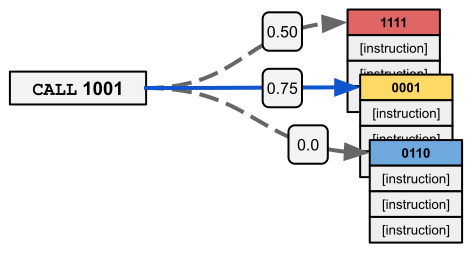
\includegraphics{./media/tag-based-referencing.png}
\caption{Example of tag-based referencing.}
\end{figure}

In the tag-based referencing example above, the call instruction uses tag 1001 to reference the closest-matching module (in this case, the yellow module tagged 0001).

\hypertarget{tag-based-regulation}{%
\subsection{Tag-based Regulation}\label{tag-based-regulation}}

Tag-based regulation allows evolving programs to instantiate gene regulatory networks using tag-based referencing.
This functionality allows programs to dynamically adjust which module is triggered by a particular call based on prior inputs.
Specifically, we implemented tag-based genetic regulation in the context of a linear GP system (SignalGP); however, our approach is applicable to any tag-enabled GP system.

To implement tag-based genetic regulation, we supplement the instruction set with promoter and repressor instructions that, when executed, adjust how well subsequent tag-based references match with a target module.
Intuitively, promoters increase a target module's tag-match score with subsequent references, thereby increasing its chances of being triggered; repressors have the opposite effect.
When determining which module to reference in response to a call instruction, each module's tag-match score is a function of how well the module's tag matches the call instruction's tag as well as the module's regulatory value.

\hypertarget{signalgp}{%
\subsection{SignalGP}\label{signalgp}}

\begin{figure}
\centering
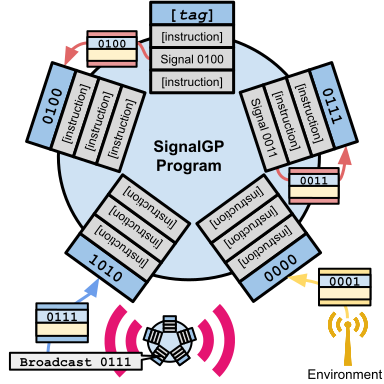
\includegraphics{./media/sgp-cartoon.png}
\caption{Cartoon overview of SignalGP.}
\end{figure}

SignalGP defines a way of organizing and interpreting genetic programs to afford computational evolution access to the \href{https://en.wikipedia.org/wiki/Event-driven_programming}{event-driven programming paradigm}.
In SignalGP, program execution is signal-driven.
Programs are segmented into genetic modules (or functions), and each module can be independently triggered in response to a signal.
Each module associates a tag with a linear sequence of instructions.
In this work, tags are represented as fixed-length bit strings.

SignalGP makes the concept of events or signals explicit: all signals contain a tag and any associated
data.
Signals can originate exogenously (e.g, from the environment or other agents) or endogenously (e.g., self-signaling).
We use tag-based referencing to determine the most appropriate function to automatically trigger in
response to a signal.
Signals trigger the function with the closest matching tag.

For a more detailed description of the SignalGP representation, see \citep{lalejini_evolving_2018}.

\hypertarget{genetic-regulation-in-signalgp}{%
\subsubsection{Genetic Regulation in SignalGP}\label{genetic-regulation-in-signalgp}}

In this work, we augment the SignalGP representation with genetic regulation, allowing programs to alter their responses to signals during their lifetime.
We supplement the SignalGP instruction set with promotor and repressor instructions, which, when executed, adjust how well subsequent signals or internal call instructions match with a target function (instruction-level tags and tag-based referencing are used for function targeting).

A simple example of how genetic regulation works (in an event-handling context) is given in the figure below. First (1), an event triggers the yellow function that, when executed, (2) promotes the red function and represses itself. Finally (3), when a subsequent signal (identical to the previous) is received, it triggers the up-regulated red function instead of the yellow function.

\begin{figure}
\centering
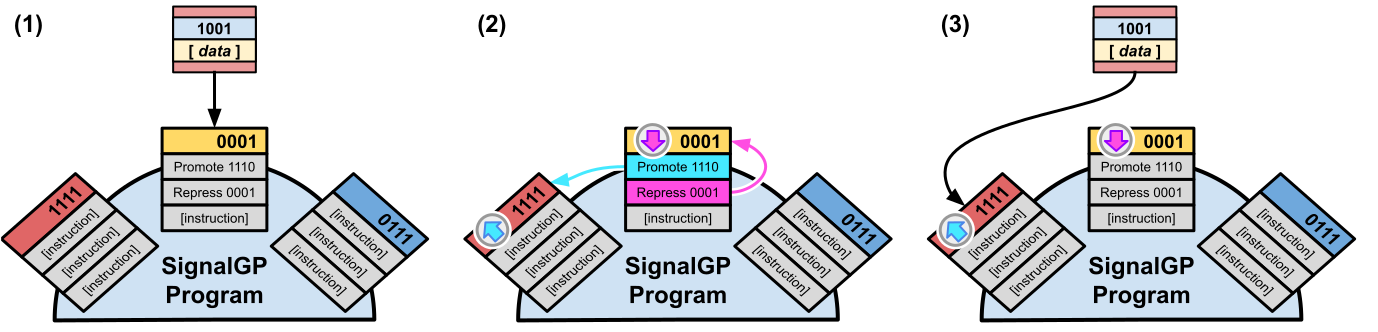
\includegraphics{./media/regulation-example-cartoon.png}
\caption{Example of tag-based genetic regulation in SignalGP.}
\end{figure}

\hypertarget{experiments}{%
\subsection{Experiments}\label{experiments}}

We compared the performance of regulation-enabled and regulation-disabled SignalGP on five problems:

\begin{itemize}
\tightlist
\item
  Repeated-signal Problem
\item
  Contextual-signal Problem
\item
  Changing-signal Problem
\item
  Boolean-logic Calculator Problem (prefix notation)
\item
  Boolean-logic Calculator Problem (postfix notation)
\end{itemize}

The repeated-signal, contextual-signal, and prefix notation calculator problems each required programs to dynamically adjust their responses to particular inputs over time.
The changing-signal and postfix notation calculator problems did not require programs to adjust responses to inputs over time.

\hypertarget{results}{%
\subsection{Results}\label{results}}

\begin{itemize}
\tightlist
\item
  Proof of method: we observed the evolution of programs capable of leveraging tag-based regulation to dynamically adjust module associations over time.
\item
  We found that tag-based regulation improved problem-solving performance on context-dependent problems (i.e., problems in which the appropriate response to a particular input changes over time).
\item
  We found that our implementation of tag-based regulation can impede adaptive evolution on problems that do not require programs to adjust responses to particular inputs over time.
\end{itemize}

\hypertarget{data-availability}{%
\chapter{Data Availability}\label{data-availability}}

\hypertarget{source-code}{%
\section{Source code}\label{source-code}}

The source code for this work is publicly accessible on GitHub: \url{https://github.com/amlalejini/Tag-based-Genetic-Regulation-for-LinearGP}.

\hypertarget{training-and-testing-sets}{%
\section{Training and testing sets}\label{training-and-testing-sets}}

The training and testing sets used for the Boolean calculator problem (prefix notation) and the Boolean calculator problem (postfix notation) are available for download from our OSF repository \citep{Lalejini_Moreno_Ofria_Data_2020} at \url{https://osf.io/928fx/}.

These training and testing sets can also be found in our \href{https://github.com/amlalejini/Tag-based-Genetic-Regulation-for-LinearGP}{GitHub repository} under the given experiment's \texttt{hpcc} directory.

\hypertarget{experimental-results}{%
\section{Experimental results}\label{experimental-results}}

All of our experimental data is available online from our OSF respository \citep{Lalejini_Moreno_Ofria_Data_2020} at \url{https://osf.io/928fx/}.

\hypertarget{compile-and-run-experiments-locally}{%
\chapter{Compile and run experiments locally}\label{compile-and-run-experiments-locally}}

Here, we provide a brief guide to compiling and running our experiments.

Please file an \href{https://github.com/amlalejini/Tag-based-Genetic-Regulation-for-LinearGP/issues}{issue} if something is unclear or does not work.

\hypertarget{docker}{%
\section{Docker}\label{docker}}

On docker hub: \url{https://hub.docker.com/r/amlalejini/tag-based-genetic-regulation-for-gp}

\begin{verbatim}
docker pull amlalejini/tag-based-genetic-regulation-for-gp
\end{verbatim}

This will create a docker image with:

\begin{itemize}
\tightlist
\item
  all the requisite dependencies installed/downloaded
\item
  all experiments compiled
\item
  our raw data downloaded
\item
  a build of our supplemental material (which will also run all of our analyses)
\end{itemize}

To run the container interactively:

\begin{verbatim}
docker run -it --entrypoint bash amlalejini/tag-based-genetic-regulation-for-gp
\end{verbatim}

You can exit the container at any point with \texttt{ctrl-d}.

Inside the container, you should be at \texttt{/opt/Tag-based-Genetic-Regulation-for-LinearGP/}.
If you \texttt{ls} you should see something like this (maybe not exactly):

\begin{verbatim}
Dockerfile                                                       documents
Gemfile                                                          experiments
LICENSE                                                          index.Rmd
Makefile                                                         media
README.md                                                        requirements.txt
_bookdown.yml                                                    scripts
_config.yml                                                      source
_output.yml                                                      style.css
alt-signal-exp_tag-len-256_match-metric-streak_thresh-0_reg-exp  _book
bool-calc-exp_tag-len-256_match-metric-streak_thresh-0_reg-exp   supplemental.bib
build_book.sh                                                    _bookdown_files
build_exps.sh                                                    tail.Rmd
chg-env-exp_tag-len-256_match-metric-streak_thresh-0_reg-exp     tests
\end{verbatim}

The important thing is that there should be three executables (with absurdly long names):

\begin{itemize}
\tightlist
\item
  \texttt{chg-env-exp\_tag-len-256\_match-metric-streak\_thresh-0\_reg-exp}

  \begin{itemize}
  \tightlist
  \item
    Use this to run the changing-signal problem.
  \item
    To generate a default configuration file, \texttt{chg-env-exp\_tag-len-256\_match-metric-streak\_thresh-0\_reg-exp\ -\/-gen}
  \end{itemize}
\item
  \texttt{alt-signal-exp\_tag-len-256\_match-metric-streak\_thresh-0\_reg-exp}

  \begin{itemize}
  \tightlist
  \item
    Use this to run the repeated-signal problem.
  \item
    To generate a default configuration file, \texttt{alt-signal-exp\_tag-len-256\_match-metric-streak\_thresh-0\_reg-exp\ -\/-gen}
  \end{itemize}
\item
  \texttt{bool-calc-exp\_tag-len-256\_match-metric-streak\_thresh-0\_reg-exp}

  \begin{itemize}
  \tightlist
  \item
    Use this to run any of the boolean-logic calculator problems and the contextual-signal problem.
  \item
    To generate a default configuration file, \texttt{bool-calc-exp\_tag-len-256\_match-metric-streak\_thresh-0\_reg-exp\ -\/-gen}
  \end{itemize}
\end{itemize}

Find the exact configurations we used for our experiments here: \url{https://github.com/amlalejini/Tag-based-Genetic-Regulation-for-LinearGP/tree/master/experiments}

\hypertarget{manually}{%
\section{Manually}\label{manually}}

This guide assumes an Ubuntu-flavored Linux operating system. These instructions \emph{should} mostly work for MacOS; otherwise, we recommend using our Docker image or a virtual machine.

Our experiments are implemented in C++, so you'll need a modern C++ compiler capable of compiling C++17 code.

E.g., I'm using:

\begin{verbatim}
g++ (Ubuntu 10.2.0-13ubuntu1) 10.2.0
\end{verbatim}

\hypertarget{get-dependencies}{%
\subsection{Get dependencies}\label{get-dependencies}}

First, make a directory were we can put this project and all of its dependencies.

\begin{verbatim}
mkdir workspace
cd workspace
\end{verbatim}

Next, clone this repository into your new directory.

\begin{verbatim}
git clone https://github.com/amlalejini/Tag-based-Genetic-Regulation-for-LinearGP.git
\end{verbatim}

Our experiments depend on the Empirical and SignalGP libraries on GitHub.
Inside the \texttt{workspace} directory, we'll clone SignalGP and checkout the appropriate commit.

\begin{verbatim}
git clone https://github.com/amlalejini/SignalGP.git
cd SignalGP
git checkout 83d879cfdb6540862315dc454c1525ccd8054e65
cd ..
\end{verbatim}

Next, let's get Empirical (also stick this in the \texttt{workspace} directory).

\begin{verbatim}
git clone https://github.com/amlalejini/Empirical.git
cd Empirical
git checkout e72dae6490dee5caf8e5ec04a634b483d2ad4293
\end{verbatim}

We're not quite done with Empirical. We need to grab all of Empirical's dependencies. This will install \emph{all} of Empirical's dependencies, including those needed to build its documentation/tests.

\begin{verbatim}
make install-dependencies
\end{verbatim}

OR, if you don't want \emph{all} of that, instead you could do:

\begin{verbatim}
git submodule init
git submodule update
\end{verbatim}

If you don't have libssl-dev, you'll also want to install that (some of the tag-matching metrics use cryptographic hash). E.g.,

\begin{verbatim}
sudo apt-get install libssl-dev
\end{verbatim}

Now we should be good to compile the three executables that we used for our experiments. Inside \texttt{workspace/Tag-based-Genetic-Regulation-for-LinearGP/}:

\begin{verbatim}
./build_exps
\end{verbatim}

This script just sets some environment variables (e.g., to define which experiment to compile, the tag-matching metric, etc.) and runs \texttt{make\ native}.

To use a different compiler (than g++), you'll need to change \texttt{CXX\_nat} in the makefile.

This should create three executables (with absurdly long names):

\begin{itemize}
\tightlist
\item
  \texttt{chg-env-exp\_tag-len-256\_match-metric-streak\_thresh-0\_reg-exp}

  \begin{itemize}
  \tightlist
  \item
    Use this to run the changing-signal problem.
  \item
    To generate a default configuration file, \texttt{chg-env-exp\_tag-len-256\_match-metric-streak\_thresh-0\_reg-exp\ -\/-gen}
  \end{itemize}
\item
  \texttt{alt-signal-exp\_tag-len-256\_match-metric-streak\_thresh-0\_reg-exp}

  \begin{itemize}
  \tightlist
  \item
    Use this to run the repeated-signal problem.
  \item
    To generate a default configuration file, \texttt{alt-signal-exp\_tag-len-256\_match-metric-streak\_thresh-0\_reg-exp\ -\/-gen}
  \end{itemize}
\item
  \texttt{bool-calc-exp\_tag-len-256\_match-metric-streak\_thresh-0\_reg-exp}

  \begin{itemize}
  \tightlist
  \item
    Use this to run any of the boolean-logic calculator problems and the contextual-signal problem.
  \item
    To generate a default configuration file, \texttt{bool-calc-exp\_tag-len-256\_match-metric-streak\_thresh-0\_reg-exp\ -\/-gen}
  \end{itemize}
\end{itemize}

Find the exact configurations we used for our experiments here: \url{https://github.com/amlalejini/Tag-based-Genetic-Regulation-for-LinearGP/tree/master/experiments}

\hypertarget{signalgp-representation}{%
\chapter{SignalGP representation}\label{signalgp-representation}}

Here, we give more details on how we configured SignalGP for this work, including the particular instruction sets used in each experiment.
For a broad overview of SignalGP, see \citep{lalejini_evolving_2018}.
For exact configurations used in each experiment, see respective \href{https://github.com/amlalejini/Tag-based-Genetic-Regulation-for-LinearGP/tree/master/experiments}{experiment directories}.

\hypertarget{memory-model}{%
\section{Memory model}\label{memory-model}}

SignalGP programs have four types of memory buffers with which to carry out computations:

\begin{itemize}
\tightlist
\item
  Working (register) memory

  \begin{itemize}
  \tightlist
  \item
    Call-local (* thread-local) memory.
  \item
    Memory used by the majority of computation instructions.
  \end{itemize}
\item
  Input memory

  \begin{itemize}
  \tightlist
  \item
    Call-local (\& thread-local) memory.
  \item
    Read-only.
  \item
    This memory is used to specify function call arguments. When a function is called on a thread (i.e.,
    a call instruction is executed), the caller's working memory is copied into the input memory of
    the new call-state, which is created on top of the thread's call stack.
  \item
    Programs must execute explicit instructions to read from the input memory buffer (into the working
    memory buffer).
  \end{itemize}
\item
  Output memory

  \begin{itemize}
  \tightlist
  \item
    Call-local (\& thread-local) memory.
  \item
    Write-only.
  \item
    This memory is used to specify the return values of a function call.
  \item
    When a function returns to the previous call-state (i.e., the one just below it on the thread's
    call stack), positions that were set in the output buffer are returned to the caller's working memory
    buffer.
  \item
    Programs must execute explicit instructions to write to the output memory buffer (from the working
    memory buffer).
  \end{itemize}
\item
  Global memory

  \begin{itemize}
  \tightlist
  \item
    This memory buffer is shared by all executing threads. Threads must use explicit instructions to access it.
  \end{itemize}
\end{itemize}

Memory buffers are implemented as integer to double maps. Instruction use their integer arguments to specify locations in memory.
In this work, evolving programs do not have de-referencing functionality (i.e., memory pointers).

\hypertarget{mutation-operators}{%
\section{Mutation operators}\label{mutation-operators}}

\begin{itemize}
\tightlist
\item
  Single-instruction insertions

  \begin{itemize}
  \tightlist
  \item
    Applied per instruction
  \end{itemize}
\item
  Single-instruction deletions

  \begin{itemize}
  \tightlist
  \item
    Applied per instruction
  \end{itemize}
\item
  Single-instruction substitutions

  \begin{itemize}
  \tightlist
  \item
    Applied per instruction
  \end{itemize}
\item
  Single-argument substitutions

  \begin{itemize}
  \tightlist
  \item
    Applied per argument
  \end{itemize}
\item
  Slip mutations \citep{lalejini_gene_2017}

  \begin{itemize}
  \tightlist
  \item
    Applied at a per-function rate.
  \item
    Pick two random positions in function's instructions sequence: A and B
  \item
    If A \textless{} B: duplicate sequence from A to B
  \item
    If A \textgreater{} B: delete sequence from A to B
  \end{itemize}
\item
  Single-function duplications

  \begin{itemize}
  \tightlist
  \item
    Applied per-function
  \end{itemize}
\item
  Single-function deletions

  \begin{itemize}
  \tightlist
  \item
    Applied per-function
  \end{itemize}
\item
  Tag bit flips

  \begin{itemize}
  \tightlist
  \item
    Applied at a per-bit rate
  \item
    (applies to both instruction- and function-tags)
  \end{itemize}
\end{itemize}

\hypertarget{instruction-set}{%
\section{Instruction set}\label{instruction-set}}

Abbreviations:

\begin{itemize}
\tightlist
\item
  EOP: End of program
\item
  Reg: local register

  \begin{itemize}
  \tightlist
  \item
    Reg{[}0{]} indicates the value at the register specified by an instruction's first \emph{argument} (either tag-based or numeric), Reg{[}1{]} indicates the value at the register specified by an instruction's second argument, and Reg{[}2{]} indicates the value at the register specified by the instruction's third argument.
  \item
    Reg{[}0{]}, Reg{[}1{]}, \emph{etc}: Register 0, Register 1, \emph{etc.}
  \end{itemize}
\item
  Input: input buffer

  \begin{itemize}
  \tightlist
  \item
    Follows same scheme as Reg
  \end{itemize}
\item
  Output: output buffer

  \begin{itemize}
  \tightlist
  \item
    Follows same scheme as Reg
  \end{itemize}
\item
  Global: global memory buffer

  \begin{itemize}
  \tightlist
  \item
    Follows same scheme as Reg
  \end{itemize}
\item
  Arg: Instruction argument

  \begin{itemize}
  \tightlist
  \item
    Arg{[}i{]} indicates the i'th instruction argument (an integer encoded in the genome)
  \item
    E.g., Arg{[}0{]} is an instruction's first argument
  \end{itemize}
\end{itemize}

Instructions that would produce undefined behavior (e.g., division by zero) are treated as no operations.

\hypertarget{default-instructions}{%
\subsection{Default Instructions}\label{default-instructions}}

I.e., instructions used across all diagnostic tasks.

\begin{longtable}[]{@{}
  >{\raggedright\arraybackslash}p{(\columnwidth - 4\tabcolsep) * \real{0.31}}
  >{\centering\arraybackslash}p{(\columnwidth - 4\tabcolsep) * \real{0.38}}
  >{\raggedright\arraybackslash}p{(\columnwidth - 4\tabcolsep) * \real{0.31}}@{}}
\toprule
Instruction & Arguments Used & Description \\
\midrule
\endhead
\texttt{Nop} & 0 & No operation \\
\texttt{Not} & 1 & Reg{[}0{]} = !Reg{[}0{]} \\
\texttt{Inc} & 1 & Reg{[}0{]} = Reg{[}0{]} + 1 \\
\texttt{Dec} & 1 & Reg{[}0{]} = Reg{[}0{]} - 1 \\
\texttt{Add} & 3 & Reg{[}2{]} = Reg{[}0{]} + Reg{[}1{]} \\
\texttt{Sub} & 3 & Reg{[}2{]} = Reg{[}0{]} - Reg{[}1{]} \\
\texttt{Mult} & 3 & Reg{[}2{]} = Reg{[}0{]} * Reg{[}1{]} \\
\texttt{Div} & 3 & Reg{[}2{]} = Reg{[}0{]} / Reg{[}1{]} \\
\texttt{Mod} & 3 & Reg{[}2{]} = Reg{[}0{]} \% Reg{[}1{]} \\
\texttt{Nand} & 2 & Reg{[}2{]} = !(Reg{[}0{]} \& Reg{[}1{]}) \\
\texttt{TestEqu} & 3 & Reg{[}2{]} = Reg{[}0{]} == Reg{[}1{]} \\
\texttt{TestNEqu} & 3 & Reg{[}2{]} = Reg{[}0{]} != Reg{[}1{]} \\
\texttt{TestLess} & 3 & Reg{[}2{]} = Reg{[}0{]} \textless{} Reg{[}1{]} \\
\texttt{TestLessEqu} & 3 & Reg{[}2{]} = Reg{[}0{]} \textless= Reg{[}1{]} \\
\texttt{TestGreater} & 3 & Reg{[}2{]} = Reg{[}0{]} \textgreater{} Reg{[}1{]} \\
\texttt{TestGreaterEqu} & 3 & Reg{[}2{]} = Reg{[}0{]} \textgreater= Reg{[}1{]} \\
\texttt{SetMem} & 2 & Reg{[}0{]} = Arg{[}1{]} \\
\texttt{Terminal} & 1 & Reg{[}0{]} = double value encoded by instruction tag \\
\texttt{CopyMem} & 2 & Reg{[}0{]} = Reg{[}1{]} \\
\texttt{SwapMem} & 2 & Swap(Reg{[}0{]}, Reg{[}1{]}) \\
\texttt{InputToWorking} & 2 & Reg{[}1{]} = Input{[}0{]} \\
\texttt{WorkingToOutput} & 2 & Output{[}1{]} = Reg{[}0{]} \\
\texttt{If} & 1 & If Reg{[}0{]} != 0, proceed. Otherwise skip to the next \texttt{Close} or EOP. \\
\texttt{While} & 1 & While Reg{[}0{]} != 0, loop. Otherwise skip to next \texttt{Close} or EOP. \\
\texttt{Close} & 0 & Indicate the end of a control block of code (e.g., loop, if). \\
\texttt{Break} & 0 & Break out of current control flow (e.g., loop). \\
\texttt{Terminate} & 0 & Kill thread that this instruction is executing on. \\
\texttt{Fork} & 0 & Generate an internal signal (using this instruction's tag) that can trigger a function to run in parallel. \\
\texttt{Call} & 0 & Call a function, using this instruction's tag to determine which function is called. \\
\texttt{Routine} & 0 & Same as call, but local memory is shared. Sort of like a jump that will jump back when the routine ends. \\
\texttt{Return} & 0 & Return from the current function call. \\
\bottomrule
\end{longtable}

Note that \texttt{Nand} performs a bitwise operation.

\hypertarget{global-memory-access-instructions}{%
\subsection{Global memory access instructions}\label{global-memory-access-instructions}}

For experimental conditions without global memory access, these instructions are replaced with no-operation
such that the instruction set remains a constant size regardless of experimental condition.

\begin{longtable}[]{@{}
  >{\raggedright\arraybackslash}p{(\columnwidth - 4\tabcolsep) * \real{0.31}}
  >{\centering\arraybackslash}p{(\columnwidth - 4\tabcolsep) * \real{0.38}}
  >{\raggedright\arraybackslash}p{(\columnwidth - 4\tabcolsep) * \real{0.31}}@{}}
\toprule
Instruction & Arguments Used & Description \\
\midrule
\endhead
\texttt{WorkingToGlobal} & 2 & Global{[}1{]} = Reg{[}0{]} \\
\texttt{GlobalToWorking} & 2 & Reg{[}1{]} = Global{[}0{]} \\
\texttt{FullGlobalToWorking} & 0 & Copy entire global memory buffer into working memory buffer \\
\texttt{FullWorkingToGlobal} & 0 & Copy entire working memory buffer into global memory buffer \\
\bottomrule
\end{longtable}

Note that full buffer copies only copy registers that have been set (they do not necessarily stomp all over the entire destination buffer).

\hypertarget{regulation-instructions}{%
\subsection{Regulation instructions}\label{regulation-instructions}}

For experimental conditions without regulation, these instructions are replaced with no-operation
such that the instruction set remains a constant size regardless of experimental condition.

Note that several regulation instructions have a baseline and (-) version.
The (-) versions are identical to the baseline version, except that they multiply the value they are
regulating with by -1. This eliminates any bias toward either up-/down-regulation.

Also note that the emp::MatchBin (in the Empirical library) data structure that manages function regulation
is defined in terms of tag DISTANCE, not similarity. So, decreasing function regulation values decreases
the distance between potential referring tags, and thus, unintuitively, \emph{up-regulates} the function.

All tag-based referencing used by regulation instructions use unregulated, raw match scores. Thus, programs
can still up-regulate a function that was previously `turned off' with down-regulation.

\begin{longtable}[]{@{}
  >{\raggedright\arraybackslash}p{(\columnwidth - 4\tabcolsep) * \real{0.31}}
  >{\centering\arraybackslash}p{(\columnwidth - 4\tabcolsep) * \real{0.38}}
  >{\raggedright\arraybackslash}p{(\columnwidth - 4\tabcolsep) * \real{0.31}}@{}}
\toprule
Instruction & Arguments Used & Description \\
\midrule
\endhead
\texttt{SetRegulator} & 1 & Set regulation value of function (targeted with instruction tag) to Reg{[}0{]}. \\
\texttt{SetRegulator-} & 1 & Set regulation value of function (targeted with instruction tag) to -1 * Reg{[}0{]}. \\
\texttt{SetOwnRegulator} & 1 & Set regulation value of function (currently executing) to Reg{[}0{]}. \\
\texttt{SetOwnRegulator-} & 1 & Set regulation value of function (currently executing) to -1 * Reg{[}0{]}. \\
\texttt{AdjRegulator} & 1 & Regulation value of function (targeted with instruction tag) += Reg{[}0{]} \\
\texttt{AdjRegulator-} & 1 & Regulation value of function (targeted with instruction tag) -= Reg{[}0{]} \\
\texttt{AdjOwnRegulator} & 1 & Regulation value of function (currently executing) += Reg{[}0{]} \\
\texttt{AdjOwnRegulator-} & 1 & Regulation value of function (currently executing) -= Reg{[}0{]} \\
\texttt{ClearRegulator} & 0 & Clear function regulation (reset to neutral) of function targeted by instruction's tag. \\
\texttt{ClearOwnRegulator} & 0 & Clear function regulation (reset to neutral) of currently executing function \\
\texttt{SenseRegulator} & 1 & Reg{[}0{]} = regulator state of function targeted by instruction tag \\
\texttt{SenseOwnRegulator} & 1 & Reg{[}0{]} = regulator state of current function \\
\texttt{IncRegulator} & 0 & Increment regulator state of function targeted with this instruction's tag \\
\texttt{IncOwnRegulator} & 0 & Increment regulator state of currently executing function \\
\texttt{DecRegulator} & 0 & Decrement regulator state of function targeted with this instruction's tag \\
\texttt{DecOwnRegulator} & 0 & Decrement regulator state of the currently executing function \\
\bottomrule
\end{longtable}

\hypertarget{task-specific-instructions}{%
\subsection{Task-specific instructions}\label{task-specific-instructions}}

Each task as a number of response instructions added to the instruction set equal to the possible set
of responses that can be expressed by a program. Each of these response instructions set a
flag on the virtual hardware indicating which response the program expressed and reset all executing
threads such that only function regulation and global memory contents persist.

\hypertarget{exponential-regulator}{%
\chapter{Exponential regulator}\label{exponential-regulator}}

For this work we used a simple exponential function to apply regulatory modifiers to tag-match scores (see details in paper).

\hypertarget{analysis-dependencies}{%
\section{Analysis Dependencies}\label{analysis-dependencies}}

Load all required R libraries.

\begin{Shaded}
\begin{Highlighting}[]
\FunctionTok{library}\NormalTok{(ggplot2)}
\FunctionTok{library}\NormalTok{(tidyverse)}
\FunctionTok{library}\NormalTok{(cowplot)}
\FunctionTok{library}\NormalTok{(viridis)}
\FunctionTok{library}\NormalTok{(RColorBrewer)}
\end{Highlighting}
\end{Shaded}

These analyses were conducted in the following computing environment:

\begin{Shaded}
\begin{Highlighting}[]
\FunctionTok{print}\NormalTok{(version)}
\end{Highlighting}
\end{Shaded}

\begin{verbatim}
##                _                           
## platform       x86_64-apple-darwin15.6.0   
## arch           x86_64                      
## os             darwin15.6.0                
## system         x86_64, darwin15.6.0        
## status                                     
## major          3                           
## minor          6.2                         
## year           2019                        
## month          12                          
## day            12                          
## svn rev        77560                       
## language       R                           
## version.string R version 3.6.2 (2019-12-12)
## nickname       Dark and Stormy Night
\end{verbatim}

Configuration:

\begin{Shaded}
\begin{Highlighting}[]
\FunctionTok{theme\_set}\NormalTok{(}\FunctionTok{theme\_cowplot}\NormalTok{())}
\NormalTok{output\_directory }\OtherTok{\textless{}{-}} \StringTok{"media/"}
\end{Highlighting}
\end{Shaded}

\hypertarget{regulator-modifier-equation}{%
\section{Regulator modifier equation}\label{regulator-modifier-equation}}

Below is the function we use to apply regulation to module match scores.

\begin{Shaded}
\begin{Highlighting}[]
\NormalTok{exp\_base }\OtherTok{\textless{}{-}} \FloatTok{1.1}
\CommentTok{\# Exponential regulator}
\NormalTok{exp\_regulator }\OtherTok{\textless{}{-}} \ControlFlowTok{function}\NormalTok{(raw\_match, modifier, }\AttributeTok{base=}\FloatTok{1.1}\NormalTok{) \{}
  \FunctionTok{return}\NormalTok{(raw\_match }\SpecialCharTok{*}\NormalTok{ (base}\SpecialCharTok{**}\NormalTok{modifier));}
\NormalTok{\}}
\end{Highlighting}
\end{Shaded}

\hypertarget{regulator-behavior}{%
\section{Regulator behavior}\label{regulator-behavior}}

Generate data to graph. We want to visualize regulated match scores as a function of raw tag match scores and module regulatory modifiers.

\begin{Shaded}
\begin{Highlighting}[]
\CommentTok{\# generate data to visualize}
\NormalTok{data }\OtherTok{\textless{}{-}} \FunctionTok{expand\_grid}\NormalTok{(}
  \AttributeTok{raw\_match=}\FunctionTok{seq}\NormalTok{(}\DecValTok{0}\NormalTok{, }\FloatTok{1.0}\NormalTok{, }\FloatTok{0.01}\NormalTok{),}
  \AttributeTok{reg\_modifier=}\FunctionTok{seq}\NormalTok{(}\SpecialCharTok{{-}}\DecValTok{10}\NormalTok{, }\DecValTok{10}\NormalTok{, }\FloatTok{0.1}\NormalTok{)}
\NormalTok{)}

\NormalTok{data }\OtherTok{\textless{}{-}} \FunctionTok{as.data.frame}\NormalTok{(data)}
\NormalTok{data}\SpecialCharTok{$}\NormalTok{regulated\_match }\OtherTok{\textless{}{-}} \FunctionTok{mapply}\NormalTok{(}
\NormalTok{  exp\_regulator,}
\NormalTok{  data}\SpecialCharTok{$}\NormalTok{raw\_match,}
\NormalTok{  data}\SpecialCharTok{$}\NormalTok{reg\_modifier,}
\NormalTok{  exp\_base}
\NormalTok{)}
\NormalTok{data}\SpecialCharTok{$}\NormalTok{above\_perfect }\OtherTok{\textless{}{-}}\NormalTok{ data}\SpecialCharTok{$}\NormalTok{regulated\_match }\SpecialCharTok{\textgreater{}} \FloatTok{1.0}
\end{Highlighting}
\end{Shaded}

We expect that 90\% of random pairs of tags fall between the two vertical dashed lines.

\begin{Shaded}
\begin{Highlighting}[]
\NormalTok{lower\_5 }\OtherTok{\textless{}{-}} \FloatTok{0.0579369}
\NormalTok{upper\_5 }\OtherTok{\textless{}{-}} \FloatTok{0.942063}
\FunctionTok{ggplot}\NormalTok{(data, }\FunctionTok{aes}\NormalTok{(}\AttributeTok{y=}\NormalTok{reg\_modifier, }\AttributeTok{x=}\NormalTok{raw\_match, }\AttributeTok{fill=}\NormalTok{regulated\_match)) }\SpecialCharTok{+}
  \FunctionTok{geom\_raster}\NormalTok{() }\SpecialCharTok{+}
  \FunctionTok{geom\_hline}\NormalTok{(}\AttributeTok{yintercept=}\DecValTok{0}\NormalTok{, }\AttributeTok{size=}\DecValTok{1}\NormalTok{, }\AttributeTok{color=}\StringTok{"black"}\NormalTok{) }\SpecialCharTok{+}
  \FunctionTok{geom\_vline}\NormalTok{(}\AttributeTok{xintercept=}\NormalTok{lower\_5, }\AttributeTok{size=}\DecValTok{1}\NormalTok{, }\AttributeTok{color=}\StringTok{"black"}\NormalTok{, }\AttributeTok{linetype=}\StringTok{"dashed"}\NormalTok{) }\SpecialCharTok{+}
  \FunctionTok{geom\_vline}\NormalTok{(}\AttributeTok{xintercept=}\NormalTok{upper\_5, }\AttributeTok{size=}\DecValTok{1}\NormalTok{, }\AttributeTok{color=}\StringTok{"black"}\NormalTok{, }\AttributeTok{linetype=}\StringTok{"dashed"}\NormalTok{) }\SpecialCharTok{+}
  \FunctionTok{scale\_x\_continuous}\NormalTok{(}\AttributeTok{name=}\StringTok{"Raw tag{-}match score"}\NormalTok{) }\SpecialCharTok{+}
  \FunctionTok{scale\_y\_continuous}\NormalTok{(}\AttributeTok{name=}\StringTok{"Module regulation modifier"}\NormalTok{) }\SpecialCharTok{+}
  \FunctionTok{scale\_fill\_distiller}\NormalTok{(}
    \AttributeTok{name=}\StringTok{"Regulated match:  "}\NormalTok{,}
    \AttributeTok{palette =} \StringTok{"Spectral"}
\NormalTok{  ) }\SpecialCharTok{+}
  \FunctionTok{theme}\NormalTok{(}
    \AttributeTok{legend.position =} \StringTok{"top"}\NormalTok{,}
    \AttributeTok{legend.key.width=}\FunctionTok{unit}\NormalTok{(}\FloatTok{1.5}\NormalTok{, }\StringTok{\textquotesingle{}cm\textquotesingle{}}\NormalTok{)}
\NormalTok{  ) }\SpecialCharTok{+}
  \FunctionTok{ggsave}\NormalTok{(}
    \FunctionTok{paste0}\NormalTok{(output\_directory, }\StringTok{"exp{-}reg{-}match.png"}\NormalTok{),}
    \AttributeTok{width=}\DecValTok{6}\NormalTok{,}
    \AttributeTok{height=}\DecValTok{6}
\NormalTok{  )}
\end{Highlighting}
\end{Shaded}

\includegraphics{tag-based-regulation-supplemental_files/figure-latex/unnamed-chunk-6-1.pdf}

Does a given raw match + regulatory modifier beat a perfect match (with no regulation)?

\begin{Shaded}
\begin{Highlighting}[]
\FunctionTok{ggplot}\NormalTok{(data, }\FunctionTok{aes}\NormalTok{(}\AttributeTok{y=}\NormalTok{reg\_modifier, }\AttributeTok{x=}\NormalTok{raw\_match, }\AttributeTok{fill=}\NormalTok{above\_perfect)) }\SpecialCharTok{+}
  \FunctionTok{geom\_tile}\NormalTok{() }\SpecialCharTok{+}
  \FunctionTok{ggsave}\NormalTok{(}
    \FunctionTok{paste0}\NormalTok{(output\_directory, }\StringTok{"exp{-}reg{-}match{-}above{-}perfect.png"}\NormalTok{),}
    \AttributeTok{width=}\DecValTok{10}\NormalTok{,}
    \AttributeTok{height=}\DecValTok{10}
\NormalTok{  )}
\end{Highlighting}
\end{Shaded}

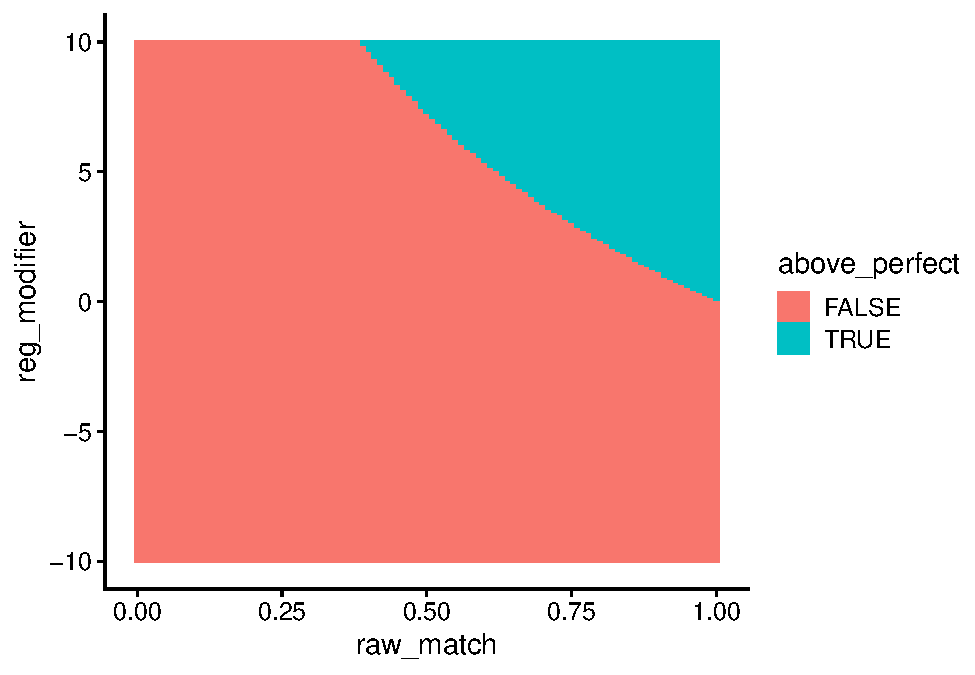
\includegraphics{tag-based-regulation-supplemental_files/figure-latex/unnamed-chunk-7-1.pdf}

\hypertarget{repeated-signal-problem-analysis}{%
\chapter{Repeated-signal problem analysis}\label{repeated-signal-problem-analysis}}

Here, we give an overview of the repeated-signal diagnostic problem, and we provide our data analyses for related experiments.
All of our source code for statistical analyses and data visualizations is embedded in this document.
The raw data can be found on the OSF project associated with this work \citep{Lalejini_Moreno_Ofria_Data_2020}.

\textbf{Please \href{https://github.com/amlalejini/Tag-based-Genetic-Regulation-for-LinearGP/issues}{file an issue or make a pull request on github} to report any mistakes, ask questions, request more explanation, et cetera.}

\hypertarget{overview}{%
\section{Overview}\label{overview}}

\begin{Shaded}
\begin{Highlighting}[]
\CommentTok{\# Experimental parameters referenced in{-}text all in one convenient place.}
\NormalTok{time\_steps }\OtherTok{\textless{}{-}} \DecValTok{128}
\NormalTok{replicates }\OtherTok{\textless{}{-}} \DecValTok{200}
\NormalTok{population\_size }\OtherTok{\textless{}{-}} \DecValTok{1000}
\NormalTok{generations }\OtherTok{\textless{}{-}} \DecValTok{10000}
\NormalTok{env\_complexities }\OtherTok{\textless{}{-}} \FunctionTok{c}\NormalTok{(}\DecValTok{2}\NormalTok{, }\DecValTok{4}\NormalTok{, }\DecValTok{8}\NormalTok{, }\DecValTok{16}\NormalTok{)}

\CommentTok{\# Settings for statistical analyses.}
\NormalTok{alpha }\OtherTok{\textless{}{-}} \FloatTok{0.05}
\NormalTok{correction\_method }\OtherTok{\textless{}{-}} \StringTok{"bonferroni"}

\CommentTok{\# Relative location of data.}
\NormalTok{working\_directory }\OtherTok{\textless{}{-}} \StringTok{"experiments/2020{-}11{-}25{-}rep{-}sig/analysis/"} \CommentTok{\# \textless{}\textless{} For bookdown}
\CommentTok{\# working\_directory \textless{}{-} "./"                                     \# \textless{}\textless{} For local analysis}
\end{Highlighting}
\end{Shaded}

The repeated-signal problem requires programs to output the appropriate (distinct) response to a single environmental signal each of the \(K\) times the signal is repeated.
Programs output responses by executing one of \(K\) response instructions.
For example, if a program receives two signals from the environment during evaluation (i.e., \(K=2\)), the program should execute \texttt{Response-1} after the first signal and \texttt{Response-2} after the second signal.

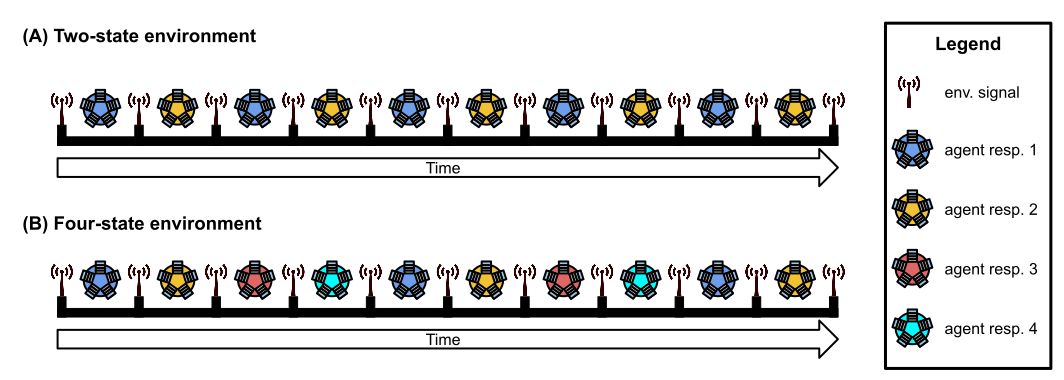
\includegraphics{experiments/2020-11-25-rep-sig/analysis/../../../media/repeated-signal-task.png}

We afford programs 128 time steps to respond to each environmental signal.
Once the allotted time expires or the program executes any response, the program's threads of execution are reset, resulting in a loss of all thread-local memory; only the contents of the global memory buffer and each program module's regulatory state persist.
The environment then produces the next signal (identical to each previous environmental signal) to which the program may respond.
A program must use the global memory buffer or genetic regulation to correctly shift its response to each subsequent environmental signal.
Evaluation continues in this way until the program correctly responds to each of the \(K\) environmental signals or until the program executes an incorrect response.
A program's fitness equals the number of correct responses given during evaluation, and a program is considered a solution if it correctly responds to each of the \(K\) environmental signals.

\hypertarget{analysis-dependencies-1}{%
\section{Analysis Dependencies}\label{analysis-dependencies-1}}

Load all required R libraries.

\begin{Shaded}
\begin{Highlighting}[]
\FunctionTok{library}\NormalTok{(ggplot2)}
\FunctionTok{library}\NormalTok{(tidyverse)}
\FunctionTok{library}\NormalTok{(reshape2)}
\FunctionTok{library}\NormalTok{(cowplot)}
\FunctionTok{library}\NormalTok{(viridis)}
\FunctionTok{library}\NormalTok{(igraph)}

\FunctionTok{source}\NormalTok{(}\StringTok{"https://gist.githubusercontent.com/benmarwick/2a1bb0133ff568cbe28d/raw/fb53bd97121f7f9ce947837ef1a4c65a73bffb3f/geom\_flat\_violin.R"}\NormalTok{)}
\end{Highlighting}
\end{Shaded}

These analyses were conducted in the following computing environment:

\begin{Shaded}
\begin{Highlighting}[]
\FunctionTok{print}\NormalTok{(version)}
\end{Highlighting}
\end{Shaded}

\begin{verbatim}
##                _                           
## platform       x86_64-apple-darwin15.6.0   
## arch           x86_64                      
## os             darwin15.6.0                
## system         x86_64, darwin15.6.0        
## status                                     
## major          3                           
## minor          6.2                         
## year           2019                        
## month          12                          
## day            12                          
## svn rev        77560                       
## language       R                           
## version.string R version 3.6.2 (2019-12-12)
## nickname       Dark and Stormy Night
\end{verbatim}

\hypertarget{setup}{%
\section{Setup}\label{setup}}

Load data, initial data cleanup, configure some global settings.

\begin{Shaded}
\begin{Highlighting}[]
\NormalTok{max\_fit\_org\_data\_loc }\OtherTok{\textless{}{-}} \FunctionTok{paste0}\NormalTok{(working\_directory, }\StringTok{"data/max\_fit\_orgs\_noprogram.csv"}\NormalTok{)}
\NormalTok{reg\_network\_data\_loc }\OtherTok{\textless{}{-}} \FunctionTok{paste0}\NormalTok{(working\_directory, }\StringTok{"data/reg\_graphs\_summary.csv"}\NormalTok{)}
\NormalTok{inst\_exec\_data\_loc }\OtherTok{\textless{}{-}} \FunctionTok{paste0}\NormalTok{(working\_directory, }\StringTok{"data/exec\_trace\_summary.csv"}\NormalTok{)}

\DocumentationTok{\#\#\#\#\#\#\# Load max fit program data \#\#\#\#\#\#\#}
\NormalTok{max\_fit\_org\_data }\OtherTok{\textless{}{-}} \FunctionTok{read.csv}\NormalTok{(max\_fit\_org\_data\_loc, }\AttributeTok{na.strings=}\StringTok{"NONE"}\NormalTok{)}

\CommentTok{\# Specify factors (not all of these matter for this set of runs).}
\NormalTok{max\_fit\_org\_data}\SpecialCharTok{$}\NormalTok{matchbin\_thresh }\OtherTok{\textless{}{-}} \FunctionTok{factor}\NormalTok{(}
\NormalTok{  max\_fit\_org\_data}\SpecialCharTok{$}\NormalTok{matchbin\_thresh,}
  \AttributeTok{levels=}\FunctionTok{c}\NormalTok{(}\DecValTok{0}\NormalTok{, }\DecValTok{25}\NormalTok{, }\DecValTok{50}\NormalTok{, }\DecValTok{75}\NormalTok{)}
\NormalTok{)}

\NormalTok{max\_fit\_org\_data}\SpecialCharTok{$}\NormalTok{NUM\_SIGNAL\_RESPONSES }\OtherTok{\textless{}{-}} \FunctionTok{factor}\NormalTok{(}
\NormalTok{  max\_fit\_org\_data}\SpecialCharTok{$}\NormalTok{NUM\_SIGNAL\_RESPONSES,}
  \AttributeTok{levels=}\FunctionTok{c}\NormalTok{(}\DecValTok{2}\NormalTok{, }\DecValTok{4}\NormalTok{, }\DecValTok{8}\NormalTok{, }\DecValTok{16}\NormalTok{, }\DecValTok{32}\NormalTok{)}
\NormalTok{)}

\NormalTok{max\_fit\_org\_data}\SpecialCharTok{$}\NormalTok{NUM\_ENV\_CYCLES }\OtherTok{\textless{}{-}} \FunctionTok{factor}\NormalTok{(}
\NormalTok{  max\_fit\_org\_data}\SpecialCharTok{$}\NormalTok{NUM\_ENV\_CYCLES,}
  \AttributeTok{levels=}\FunctionTok{c}\NormalTok{(}\DecValTok{2}\NormalTok{, }\DecValTok{4}\NormalTok{, }\DecValTok{8}\NormalTok{, }\DecValTok{16}\NormalTok{, }\DecValTok{32}\NormalTok{)}
\NormalTok{)}

\NormalTok{max\_fit\_org\_data}\SpecialCharTok{$}\NormalTok{TAG\_LEN }\OtherTok{\textless{}{-}} \FunctionTok{factor}\NormalTok{(}
\NormalTok{  max\_fit\_org\_data}\SpecialCharTok{$}\NormalTok{TAG\_LEN,}
  \AttributeTok{levels=}\FunctionTok{c}\NormalTok{(}\DecValTok{32}\NormalTok{, }\DecValTok{64}\NormalTok{, }\DecValTok{128}\NormalTok{, }\DecValTok{256}\NormalTok{)}
\NormalTok{)}

\CommentTok{\# Define function to summarize regulation/memory configurations.}
\NormalTok{get\_con }\OtherTok{\textless{}{-}} \ControlFlowTok{function}\NormalTok{(reg, mem) \{}
  \ControlFlowTok{if}\NormalTok{ (reg }\SpecialCharTok{==} \StringTok{"0"} \SpecialCharTok{\&\&}\NormalTok{ mem }\SpecialCharTok{==} \StringTok{"0"}\NormalTok{) \{}
    \FunctionTok{return}\NormalTok{(}\StringTok{"none"}\NormalTok{)}
\NormalTok{  \} }\ControlFlowTok{else} \ControlFlowTok{if}\NormalTok{ (reg }\SpecialCharTok{==} \StringTok{"0"} \SpecialCharTok{\&\&}\NormalTok{ mem}\SpecialCharTok{==}\StringTok{"1"}\NormalTok{) \{}
    \FunctionTok{return}\NormalTok{(}\StringTok{"memory"}\NormalTok{)}
\NormalTok{  \} }\ControlFlowTok{else} \ControlFlowTok{if}\NormalTok{ (reg}\SpecialCharTok{==}\StringTok{"1"} \SpecialCharTok{\&\&}\NormalTok{ mem}\SpecialCharTok{==}\StringTok{"0"}\NormalTok{) \{}
    \FunctionTok{return}\NormalTok{(}\StringTok{"regulation"}\NormalTok{)}
\NormalTok{  \} }\ControlFlowTok{else} \ControlFlowTok{if}\NormalTok{ (reg}\SpecialCharTok{==}\StringTok{"1"} \SpecialCharTok{\&\&}\NormalTok{ mem}\SpecialCharTok{==}\StringTok{"1"}\NormalTok{) \{}
    \FunctionTok{return}\NormalTok{(}\StringTok{"both"}\NormalTok{)}
\NormalTok{  \} }\ControlFlowTok{else}\NormalTok{ \{}
    \FunctionTok{return}\NormalTok{(}\StringTok{"UNKNOWN"}\NormalTok{)}
\NormalTok{  \}}
\NormalTok{\}}

\CommentTok{\# Specify experimental condition for each datum.}
\NormalTok{max\_fit\_org\_data}\SpecialCharTok{$}\NormalTok{condition }\OtherTok{\textless{}{-}} \FunctionTok{mapply}\NormalTok{(}
\NormalTok{  get\_con,}
\NormalTok{  max\_fit\_org\_data}\SpecialCharTok{$}\NormalTok{USE\_FUNC\_REGULATION,}
\NormalTok{  max\_fit\_org\_data}\SpecialCharTok{$}\NormalTok{USE\_GLOBAL\_MEMORY}
\NormalTok{)}

\NormalTok{max\_fit\_org\_data}\SpecialCharTok{$}\NormalTok{condition }\OtherTok{\textless{}{-}} \FunctionTok{factor}\NormalTok{(}
\NormalTok{  max\_fit\_org\_data}\SpecialCharTok{$}\NormalTok{condition,}
  \AttributeTok{levels=}\FunctionTok{c}\NormalTok{(}\StringTok{"regulation"}\NormalTok{, }\StringTok{"memory"}\NormalTok{, }\StringTok{"none"}\NormalTok{, }\StringTok{"both"}\NormalTok{)}
\NormalTok{)}

\CommentTok{\# Does this program rely on a stochastic strategy?}
\NormalTok{max\_fit\_org\_data}\SpecialCharTok{$}\NormalTok{stochastic }\OtherTok{\textless{}{-}} \DecValTok{1} \SpecialCharTok{{-}}\NormalTok{ max\_fit\_org\_data}\SpecialCharTok{$}\NormalTok{consistent}

\NormalTok{max\_fit\_org\_data}\SpecialCharTok{$}\NormalTok{stochastic }\OtherTok{\textless{}{-}} \FunctionTok{factor}\NormalTok{(}
\NormalTok{  max\_fit\_org\_data}\SpecialCharTok{$}\NormalTok{stochastic,}
  \AttributeTok{levels=}\FunctionTok{c}\NormalTok{(}\DecValTok{0}\NormalTok{, }\DecValTok{1}\NormalTok{)}
\NormalTok{)}

\CommentTok{\# Filter data to include only runs from regulation{-}enabled (\textquotesingle{}both\textquotesingle{}) and regulation{-}disabled (\textquotesingle{}memory\textquotesingle{}) conditions}
\NormalTok{max\_fit\_org\_data }\OtherTok{\textless{}{-}} \FunctionTok{filter}\NormalTok{(max\_fit\_org\_data, condition }\SpecialCharTok{\%in\%} \FunctionTok{c}\NormalTok{(}\StringTok{"both"}\NormalTok{, }\StringTok{"memory"}\NormalTok{))}

\CommentTok{\# Filter data to include only replicates labeled as solutions}
\NormalTok{sol\_data }\OtherTok{\textless{}{-}} \FunctionTok{filter}\NormalTok{(max\_fit\_org\_data, solution}\SpecialCharTok{==}\StringTok{"1"}\NormalTok{)}

\CommentTok{\# Label solution strategies}
\NormalTok{get\_strategy }\OtherTok{\textless{}{-}} \ControlFlowTok{function}\NormalTok{(use\_reg, use\_mem) \{}
  \ControlFlowTok{if}\NormalTok{ (use\_reg}\SpecialCharTok{==}\StringTok{"0"} \SpecialCharTok{\&\&}\NormalTok{ use\_mem}\SpecialCharTok{==}\StringTok{"0"}\NormalTok{) \{}
    \FunctionTok{return}\NormalTok{(}\StringTok{"use neither"}\NormalTok{)}
\NormalTok{  \} }\ControlFlowTok{else} \ControlFlowTok{if}\NormalTok{ (use\_reg}\SpecialCharTok{==}\StringTok{"0"} \SpecialCharTok{\&\&}\NormalTok{ use\_mem}\SpecialCharTok{==}\StringTok{"1"}\NormalTok{) \{}
    \FunctionTok{return}\NormalTok{(}\StringTok{"use memory"}\NormalTok{)}
\NormalTok{  \} }\ControlFlowTok{else} \ControlFlowTok{if}\NormalTok{ (use\_reg}\SpecialCharTok{==}\StringTok{"1"} \SpecialCharTok{\&\&}\NormalTok{ use\_mem}\SpecialCharTok{==}\StringTok{"0"}\NormalTok{) \{}
    \FunctionTok{return}\NormalTok{(}\StringTok{"use regulation"}\NormalTok{)}
\NormalTok{  \} }\ControlFlowTok{else} \ControlFlowTok{if}\NormalTok{ (use\_reg}\SpecialCharTok{==}\StringTok{"1"} \SpecialCharTok{\&\&}\NormalTok{ use\_mem}\SpecialCharTok{==}\StringTok{"1"}\NormalTok{) \{}
    \FunctionTok{return}\NormalTok{(}\StringTok{"use both"}\NormalTok{)}
\NormalTok{  \} }\ControlFlowTok{else}\NormalTok{ \{}
    \FunctionTok{return}\NormalTok{(}\StringTok{"UNKNOWN"}\NormalTok{)}
\NormalTok{  \}}
\NormalTok{\}}

\CommentTok{\# Specify experimental conditions (to make labeling easier).}
\NormalTok{sol\_data}\SpecialCharTok{$}\NormalTok{strategy }\OtherTok{\textless{}{-}}  \FunctionTok{mapply}\NormalTok{(}
\NormalTok{  get\_strategy,}
\NormalTok{  sol\_data}\SpecialCharTok{$}\NormalTok{relies\_on\_regulation,}
\NormalTok{  sol\_data}\SpecialCharTok{$}\NormalTok{relies\_on\_global\_memory}
\NormalTok{)}

\NormalTok{sol\_data}\SpecialCharTok{$}\NormalTok{strategy }\OtherTok{\textless{}{-}} \FunctionTok{factor}\NormalTok{(}
\NormalTok{  sol\_data}\SpecialCharTok{$}\NormalTok{strategy,}
  \AttributeTok{levels=}\FunctionTok{c}\NormalTok{(}
    \StringTok{"use regulation"}\NormalTok{,}
    \StringTok{"use memory"}\NormalTok{,}
    \StringTok{"use neither"}\NormalTok{,}
    \StringTok{"use both"}
\NormalTok{  )}
\NormalTok{)}

\DocumentationTok{\#\#\#\#\#\#\# Load network data \#\#\#\#\#\#\#}
\NormalTok{reg\_network\_data }\OtherTok{\textless{}{-}} \FunctionTok{read.csv}\NormalTok{(reg\_network\_data\_loc, }\AttributeTok{na.strings=}\StringTok{"NA"}\NormalTok{)}
\NormalTok{reg\_network\_data }\OtherTok{\textless{}{-}} \FunctionTok{filter}\NormalTok{(reg\_network\_data, run\_id }\SpecialCharTok{\%in\%}\NormalTok{ max\_fit\_org\_data}\SpecialCharTok{$}\NormalTok{SEED)}

\CommentTok{\# Make a lookup function to get each run\textquotesingle{}s environment complexity level.}
\NormalTok{get\_num\_sig\_resps }\OtherTok{\textless{}{-}} \ControlFlowTok{function}\NormalTok{(seed) \{}
  \FunctionTok{return}\NormalTok{(}\FunctionTok{filter}\NormalTok{(max\_fit\_org\_data, SEED}\SpecialCharTok{==}\NormalTok{seed)}\SpecialCharTok{$}\NormalTok{NUM\_SIGNAL\_RESPONSES)}
\NormalTok{\}}

\NormalTok{reg\_network\_data}\SpecialCharTok{$}\NormalTok{NUM\_SIGNAL\_RESPONSES }\OtherTok{\textless{}{-}} \FunctionTok{mapply}\NormalTok{(}
\NormalTok{  get\_num\_sig\_resps,}
\NormalTok{  reg\_network\_data}\SpecialCharTok{$}\NormalTok{run\_id}
\NormalTok{)}

\NormalTok{reg\_network\_data}\SpecialCharTok{$}\NormalTok{NUM\_SIGNAL\_RESPONSES }\OtherTok{\textless{}{-}} \FunctionTok{factor}\NormalTok{(reg\_network\_data}\SpecialCharTok{$}\NormalTok{NUM\_SIGNAL\_RESPONSES)}


\DocumentationTok{\#\#\#\#\#\#\# Load instruction execution data \#\#\#\#\#\#\#}
\NormalTok{inst\_exec\_data }\OtherTok{\textless{}{-}} \FunctionTok{read.csv}\NormalTok{(inst\_exec\_data\_loc, }\AttributeTok{na.strings=}\StringTok{"NA"}\NormalTok{)}

\NormalTok{inst\_exec\_data}\SpecialCharTok{$}\NormalTok{condition }\OtherTok{\textless{}{-}} \FunctionTok{mapply}\NormalTok{(}
\NormalTok{  get\_con,}
\NormalTok{  inst\_exec\_data}\SpecialCharTok{$}\NormalTok{USE\_FUNC\_REGULATION,}
\NormalTok{  inst\_exec\_data}\SpecialCharTok{$}\NormalTok{USE\_GLOBAL\_MEMORY}
\NormalTok{)}

\NormalTok{inst\_exec\_data}\SpecialCharTok{$}\NormalTok{condition }\OtherTok{\textless{}{-}} \FunctionTok{factor}\NormalTok{(}
\NormalTok{  inst\_exec\_data}\SpecialCharTok{$}\NormalTok{condition,}
  \AttributeTok{levels=}\FunctionTok{c}\NormalTok{(}\StringTok{"regulation"}\NormalTok{, }\StringTok{"memory"}\NormalTok{, }\StringTok{"none"}\NormalTok{, }\StringTok{"both"}\NormalTok{)}
\NormalTok{)}

\NormalTok{inst\_exec\_data}\SpecialCharTok{$}\NormalTok{NUM\_SIGNAL\_RESPONSES }\OtherTok{\textless{}{-}} \FunctionTok{factor}\NormalTok{(}
\NormalTok{  inst\_exec\_data}\SpecialCharTok{$}\NormalTok{NUM\_SIGNAL\_RESPONSES,}
  \AttributeTok{levels=}\FunctionTok{c}\NormalTok{(}\DecValTok{2}\NormalTok{, }\DecValTok{4}\NormalTok{, }\DecValTok{8}\NormalTok{, }\DecValTok{16}\NormalTok{, }\DecValTok{32}\NormalTok{)}
\NormalTok{)}

\NormalTok{inst\_exec\_data}\SpecialCharTok{$}\NormalTok{NUM\_ENV\_CYCLES }\OtherTok{\textless{}{-}} \FunctionTok{factor}\NormalTok{(}
\NormalTok{  inst\_exec\_data}\SpecialCharTok{$}\NormalTok{NUM\_ENV\_CYCLES,}
  \AttributeTok{levels=}\FunctionTok{c}\NormalTok{(}\DecValTok{2}\NormalTok{, }\DecValTok{4}\NormalTok{, }\DecValTok{8}\NormalTok{, }\DecValTok{16}\NormalTok{, }\DecValTok{32}\NormalTok{)}
\NormalTok{)}

\CommentTok{\# Labels for each}
\NormalTok{label\_lu }\OtherTok{\textless{}{-}} \FunctionTok{c}\NormalTok{(}
  \StringTok{"2"} \OtherTok{=} \StringTok{"2{-}signal task"}\NormalTok{,}
  \StringTok{"4"} \OtherTok{=} \StringTok{"4{-}signal task"}\NormalTok{,}
  \StringTok{"8"} \OtherTok{=} \StringTok{"8{-}signal task"}\NormalTok{,}
  \StringTok{"16"} \OtherTok{=} \StringTok{"16{-}signal task"}\NormalTok{,}
  \StringTok{"32"} \OtherTok{=}\StringTok{"32{-}signal task"}
\NormalTok{)}

\DocumentationTok{\#\#\#\#\#\#\# misc \#\#\#\#\#\#\#}
\CommentTok{\# Configure our default graphing theme}
\FunctionTok{theme\_set}\NormalTok{(}\FunctionTok{theme\_cowplot}\NormalTok{())}
\end{Highlighting}
\end{Shaded}

\hypertarget{problem-solving-success}{%
\section{Problem-solving success}\label{problem-solving-success}}

We expected populations with access to genetic regulation to be more successful on the repeated-signal task than those evolved without access to genetic regulation.
Further, we expected the success differential to increase with problem difficulty.

We can look at
(1) the number of successful replicates (i.e., replicates in which a program capable of perfectly solving the repeated signal task evolved) per condition
and (2) the scores of the highest-fitness program evolved in each replicate.

\hypertarget{number-of-successful-replicates-by-condition}{%
\subsection{Number of successful replicates by condition}\label{number-of-successful-replicates-by-condition}}

Note that a program is categorized as a `solution' only if it can correctly respond to each of repetition of the environment signal.

\begin{Shaded}
\begin{Highlighting}[]
\CommentTok{\# Graph the number of solutions evolved in each condition, faceted by environmental complexity}
\FunctionTok{ggplot}\NormalTok{( sol\_data, }\FunctionTok{aes}\NormalTok{(}\AttributeTok{x=}\NormalTok{condition, }\AttributeTok{fill=}\NormalTok{condition) ) }\SpecialCharTok{+}
  \FunctionTok{geom\_bar}\NormalTok{() }\SpecialCharTok{+}
  \FunctionTok{geom\_text}\NormalTok{(}
    \AttributeTok{stat=}\StringTok{"count"}\NormalTok{,}
    \AttributeTok{mapping=}\FunctionTok{aes}\NormalTok{(}\AttributeTok{label=}\NormalTok{..count..),}
    \AttributeTok{position=}\FunctionTok{position\_dodge}\NormalTok{(}\FloatTok{0.9}\NormalTok{),}
    \AttributeTok{vjust=}\DecValTok{0}
\NormalTok{  ) }\SpecialCharTok{+}
  \FunctionTok{scale\_y\_continuous}\NormalTok{(}
    \AttributeTok{name=}\StringTok{"\# evolved solutions"}\NormalTok{,}
    \AttributeTok{breaks=}\FunctionTok{seq}\NormalTok{(}\DecValTok{0}\NormalTok{, replicates, }\DecValTok{50}\NormalTok{),}
    \AttributeTok{limits=}\FunctionTok{c}\NormalTok{(}\DecValTok{0}\NormalTok{, replicates}\SpecialCharTok{+}\DecValTok{2}\NormalTok{)}
\NormalTok{  ) }\SpecialCharTok{+}
  \FunctionTok{scale\_fill\_discrete}\NormalTok{(}
    \AttributeTok{name=}\StringTok{"Condition:"}\NormalTok{,}
    \AttributeTok{limits=}\FunctionTok{c}\NormalTok{(}\StringTok{"memory"}\NormalTok{, }\StringTok{"both"}\NormalTok{),}
    \AttributeTok{labels=}\FunctionTok{c}\NormalTok{(}\StringTok{"Regulation{-}disabled (D)"}\NormalTok{, }\StringTok{"Regulation{-}enabled (E)"}\NormalTok{)}
\NormalTok{  ) }\SpecialCharTok{+}
  \FunctionTok{scale\_x\_discrete}\NormalTok{(}
    \AttributeTok{name=}\StringTok{"Condition"}\NormalTok{,}
    \AttributeTok{limits=}\FunctionTok{c}\NormalTok{(}\StringTok{"memory"}\NormalTok{, }\StringTok{"both"}\NormalTok{),}
    \AttributeTok{labels=}\FunctionTok{c}\NormalTok{(}\StringTok{"D"}\NormalTok{, }\StringTok{"E"}\NormalTok{)}
\NormalTok{  ) }\SpecialCharTok{+}
  \FunctionTok{facet\_wrap}\NormalTok{(}
    \SpecialCharTok{\textasciitilde{}}\NormalTok{ NUM\_SIGNAL\_RESPONSES,}
    \AttributeTok{nrow=}\DecValTok{1}\NormalTok{,}
    \AttributeTok{labeller=}\FunctionTok{labeller}\NormalTok{(}\AttributeTok{NUM\_SIGNAL\_RESPONSES=}\NormalTok{label\_lu)}
\NormalTok{  ) }\SpecialCharTok{+}
  \FunctionTok{ggtitle}\NormalTok{(}\StringTok{"Solution Counts"}\NormalTok{) }\SpecialCharTok{+}
  \FunctionTok{theme}\NormalTok{(}
    \AttributeTok{legend.position=}\StringTok{"bottom"}\NormalTok{,}
    \AttributeTok{axis.title.x=}\FunctionTok{element\_blank}\NormalTok{()}
\NormalTok{  ) }\SpecialCharTok{+}
  \FunctionTok{ggsave}\NormalTok{(}
    \FunctionTok{paste0}\NormalTok{(working\_directory, }\StringTok{"imgs/repeated{-}signal{-}solultion{-}cnts.png"}\NormalTok{),}
    \AttributeTok{width=}\DecValTok{8}\NormalTok{,}
    \AttributeTok{height=}\DecValTok{4}
\NormalTok{  )}
\end{Highlighting}
\end{Shaded}

\includegraphics{tag-based-regulation-supplemental_files/figure-latex/unnamed-chunk-12-1.pdf}

We confirmed that each difficulty level of the repeated-signal problem is solvable without regulation using \href{https://github.com/amlalejini/Tag-based-Genetic-Regulation-for-LinearGP/blob/master/documents/handcoded-examples.md}{hand-coded SignalGP programs}.

We use a Fisher's exact test to determine if there are significant differences (p \textless{} 0.05) between the numbers of regulation-enabled versus regulation-disabled solutions for each problem difficulty.

\begin{Shaded}
\begin{Highlighting}[]
\CommentTok{\# This code chunk is sort of a monster to have things print out all pretty{-}like in the knitted HTML document.}

\CommentTok{\# For each environment complexity level, do a fisher\textquotesingle{}s exact test and print results.}
\ControlFlowTok{for}\NormalTok{ (env }\ControlFlowTok{in}\NormalTok{ env\_complexities) \{}
\NormalTok{  env\_data }\OtherTok{\textless{}{-}} \FunctionTok{filter}\NormalTok{(max\_fit\_org\_data, NUM\_SIGNAL\_RESPONSES}\SpecialCharTok{==}\NormalTok{env)}
  \FunctionTok{cat}\NormalTok{(}\StringTok{"\#\#\#\# "}\NormalTok{, }\FunctionTok{paste0}\NormalTok{(env, }\StringTok{"{-}signal task"}\NormalTok{), }\StringTok{" {-} statistical analysis of solution counts  }\SpecialCharTok{\textbackslash{}n}\StringTok{"}\NormalTok{)}

  \CommentTok{\# Extract successes/fails for each condition.}
\NormalTok{  mem\_success\_cnt }\OtherTok{\textless{}{-}} \FunctionTok{nrow}\NormalTok{(}\FunctionTok{filter}\NormalTok{(env\_data, solution}\SpecialCharTok{==}\StringTok{"1"} \SpecialCharTok{\&}\NormalTok{ condition}\SpecialCharTok{==}\StringTok{"memory"}\NormalTok{))}
\NormalTok{  mem\_fail\_cnt }\OtherTok{\textless{}{-}} \FunctionTok{nrow}\NormalTok{(}\FunctionTok{filter}\NormalTok{(env\_data, condition}\SpecialCharTok{==}\StringTok{"memory"}\NormalTok{)) }\SpecialCharTok{{-}}\NormalTok{ mem\_success\_cnt}
\NormalTok{  both\_success\_cnt }\OtherTok{\textless{}{-}} \FunctionTok{nrow}\NormalTok{(}\FunctionTok{filter}\NormalTok{(env\_data, solution}\SpecialCharTok{==}\StringTok{"1"} \SpecialCharTok{\&}\NormalTok{ condition}\SpecialCharTok{==}\StringTok{"both"}\NormalTok{))}
\NormalTok{  both\_fail\_cnt }\OtherTok{\textless{}{-}} \FunctionTok{nrow}\NormalTok{(}\FunctionTok{filter}\NormalTok{(env\_data, condition}\SpecialCharTok{==}\StringTok{"both"}\NormalTok{)) }\SpecialCharTok{{-}}\NormalTok{ both\_success\_cnt}

  \CommentTok{\# Regulation{-}disabled vs regulation{-}enabled}
\NormalTok{  mem\_sgp\_table }\OtherTok{\textless{}{-}} \FunctionTok{matrix}\NormalTok{(}\FunctionTok{c}\NormalTok{(both\_success\_cnt,}
\NormalTok{                            mem\_success\_cnt,}
\NormalTok{                            both\_fail\_cnt,}
\NormalTok{                            mem\_fail\_cnt),}
                          \AttributeTok{nrow=}\DecValTok{2}\NormalTok{)}
  \FunctionTok{rownames}\NormalTok{(mem\_sgp\_table) }\OtherTok{\textless{}{-}} \FunctionTok{c}\NormalTok{(}\StringTok{"reg{-}enabled"}\NormalTok{, }\StringTok{"reg{-}disabled"}\NormalTok{)}
  \FunctionTok{colnames}\NormalTok{(mem\_sgp\_table) }\OtherTok{\textless{}{-}} \FunctionTok{c}\NormalTok{(}\StringTok{"success"}\NormalTok{, }\StringTok{"fail"}\NormalTok{)}
\NormalTok{  mem\_sgp\_fishers }\OtherTok{\textless{}{-}} \FunctionTok{fisher.test}\NormalTok{(mem\_sgp\_table)}

  \FunctionTok{cat}\NormalTok{(}\StringTok{"}\SpecialCharTok{\textbackslash{}n}\StringTok{"}\NormalTok{)}
  \FunctionTok{cat}\NormalTok{(}\StringTok{"Regulation{-}enabled SignalGP vs. regulation{-}disabled SignalGP (original version of SignalGP):  }\SpecialCharTok{\textbackslash{}n}\StringTok{"}\NormalTok{)}
  \FunctionTok{cat}\NormalTok{(}\StringTok{"\textasciigrave{}\textasciigrave{}\textasciigrave{}}\SpecialCharTok{\textbackslash{}n}\StringTok{"}\NormalTok{)}
  \FunctionTok{print}\NormalTok{(mem\_sgp\_table)}
  \FunctionTok{print}\NormalTok{(mem\_sgp\_fishers)}
  \FunctionTok{cat}\NormalTok{(}\StringTok{"\textasciigrave{}\textasciigrave{}\textasciigrave{}}\SpecialCharTok{\textbackslash{}n}\StringTok{"}\NormalTok{)}
  \FunctionTok{cat}\NormalTok{(}\StringTok{"}\SpecialCharTok{\textbackslash{}n}\StringTok{"}\NormalTok{)}
\NormalTok{\}}
\end{Highlighting}
\end{Shaded}

\hypertarget{signal-task---statistical-analysis-of-solution-counts}{%
\subsubsection{2-signal task - statistical analysis of solution counts}\label{signal-task---statistical-analysis-of-solution-counts}}

Regulation-enabled SignalGP vs.~regulation-disabled SignalGP (original version of SignalGP):

\begin{verbatim}
             success fail
reg-enabled      200    0
reg-disabled     137   63

    Fisher's Exact Test for Count Data

data:  mem_sgp_table
p-value < 2.2e-16
alternative hypothesis: true odds ratio is not equal to 1
95 percent confidence interval:
 23.54182      Inf
sample estimates:
odds ratio 
       Inf 
\end{verbatim}

\hypertarget{signal-task---statistical-analysis-of-solution-counts-1}{%
\subsubsection{4-signal task - statistical analysis of solution counts}\label{signal-task---statistical-analysis-of-solution-counts-1}}

Regulation-enabled SignalGP vs.~regulation-disabled SignalGP (original version of SignalGP):

\begin{verbatim}
             success fail
reg-enabled      200    0
reg-disabled       8  192

    Fisher's Exact Test for Count Data

data:  mem_sgp_table
p-value < 2.2e-16
alternative hypothesis: true odds ratio is not equal to 1
95 percent confidence interval:
 953.6049      Inf
sample estimates:
odds ratio 
       Inf 
\end{verbatim}

\hypertarget{signal-task---statistical-analysis-of-solution-counts-2}{%
\subsubsection{8-signal task - statistical analysis of solution counts}\label{signal-task---statistical-analysis-of-solution-counts-2}}

Regulation-enabled SignalGP vs.~regulation-disabled SignalGP (original version of SignalGP):

\begin{verbatim}
             success fail
reg-enabled      198    2
reg-disabled       0  200

    Fisher's Exact Test for Count Data

data:  mem_sgp_table
p-value < 2.2e-16
alternative hypothesis: true odds ratio is not equal to 1
95 percent confidence interval:
 2409.412      Inf
sample estimates:
odds ratio 
       Inf 
\end{verbatim}

\hypertarget{signal-task---statistical-analysis-of-solution-counts-3}{%
\subsubsection{16-signal task - statistical analysis of solution counts}\label{signal-task---statistical-analysis-of-solution-counts-3}}

Regulation-enabled SignalGP vs.~regulation-disabled SignalGP (original version of SignalGP):

\begin{verbatim}
             success fail
reg-enabled       74  126
reg-disabled       0  200

    Fisher's Exact Test for Count Data

data:  mem_sgp_table
p-value < 2.2e-16
alternative hypothesis: true odds ratio is not equal to 1
95 percent confidence interval:
 30.12902      Inf
sample estimates:
odds ratio 
       Inf 
\end{verbatim}

\hypertarget{aggregate-fitness-scores-by-condition}{%
\subsection{Aggregate fitness scores by condition}\label{aggregate-fitness-scores-by-condition}}

Here, we visualize the raw task scores for the highest-fitness program from each run across all environments/conditions.

\begin{Shaded}
\begin{Highlighting}[]
\FunctionTok{ggplot}\NormalTok{( max\_fit\_org\_data, }\FunctionTok{aes}\NormalTok{(}\AttributeTok{x=}\NormalTok{condition, }\AttributeTok{y=}\NormalTok{score, }\AttributeTok{color=}\NormalTok{condition) ) }\SpecialCharTok{+}
  \FunctionTok{geom\_boxplot}\NormalTok{() }\SpecialCharTok{+}
  \FunctionTok{geom\_jitter}\NormalTok{(}\AttributeTok{alpha=}\FloatTok{0.2}\NormalTok{) }\SpecialCharTok{+}
  \FunctionTok{ylab}\NormalTok{(}\StringTok{"Score (\# correct responses)"}\NormalTok{) }\SpecialCharTok{+}
  \FunctionTok{scale\_color\_discrete}\NormalTok{(}
    \AttributeTok{name=}\StringTok{"Condition"}\NormalTok{,}
    \AttributeTok{breaks=}\FunctionTok{c}\NormalTok{(}\StringTok{"memory"}\NormalTok{, }\StringTok{"both"}\NormalTok{),}
    \AttributeTok{labels=}\FunctionTok{c}\NormalTok{(}\StringTok{"Regulation{-}disabled (D)"}\NormalTok{, }\StringTok{"Regulation{-}enabled (E)"}\NormalTok{)}
\NormalTok{  ) }\SpecialCharTok{+}
  \FunctionTok{scale\_x\_discrete}\NormalTok{(}
    \AttributeTok{name=}\StringTok{"Condition"}\NormalTok{,}
    \AttributeTok{breaks=}\FunctionTok{c}\NormalTok{(}\StringTok{"memory"}\NormalTok{, }\StringTok{"both"}\NormalTok{),}
    \AttributeTok{labels=}\FunctionTok{c}\NormalTok{(}\StringTok{"D"}\NormalTok{, }\StringTok{"E"}\NormalTok{)}
\NormalTok{  ) }\SpecialCharTok{+}
  \FunctionTok{facet\_wrap}\NormalTok{(}
    \SpecialCharTok{\textasciitilde{}}\NormalTok{ NUM\_SIGNAL\_RESPONSES,}
    \AttributeTok{scales=}\StringTok{"free\_y"}\NormalTok{,}
    \AttributeTok{labeller=}\FunctionTok{labeller}\NormalTok{(}\AttributeTok{NUM\_SIGNAL\_RESPONSES=}\NormalTok{label\_lu)}
\NormalTok{  ) }\SpecialCharTok{+}
  \FunctionTok{theme}\NormalTok{(}
    \AttributeTok{legend.position=}\StringTok{"bottom"}\NormalTok{,}
    \AttributeTok{axis.title.x=}\FunctionTok{element\_blank}\NormalTok{()}
\NormalTok{  ) }\SpecialCharTok{+}
  \FunctionTok{ggtitle}\NormalTok{(}\StringTok{"Task Scores"}\NormalTok{) }\SpecialCharTok{+}
  \FunctionTok{ggsave}\NormalTok{(}
    \FunctionTok{paste0}\NormalTok{(working\_directory, }\StringTok{"imgs/repeated{-}signal{-}scores.png"}\NormalTok{),}
    \AttributeTok{width=}\DecValTok{16}\NormalTok{,}
    \AttributeTok{height=}\DecValTok{8}
\NormalTok{  )}
\end{Highlighting}
\end{Shaded}

\includegraphics{tag-based-regulation-supplemental_files/figure-latex/unnamed-chunk-14-1.pdf}

\hypertarget{how-many-generations-elapse-before-solutions-evolve}{%
\section{How many generations elapse before solutions evolve?}\label{how-many-generations-elapse-before-solutions-evolve}}

Do some conditions lead to the evolution of solutions in fewer generations than other conditions?

Here, we compare the generation at which solutions arise (only at difficulty levels where regulation-disabled solutions evovled).

\begin{Shaded}
\begin{Highlighting}[]
\NormalTok{unfinished\_data }\OtherTok{\textless{}{-}} \FunctionTok{filter}\NormalTok{(max\_fit\_org\_data, solution}\SpecialCharTok{==}\StringTok{"0"}\NormalTok{)}
\NormalTok{unfinished\_data}\SpecialCharTok{$}\NormalTok{graph\_update }\OtherTok{\textless{}{-}} \DecValTok{100000}

\FunctionTok{ggplot}\NormalTok{( ) }\SpecialCharTok{+}
  \FunctionTok{geom\_flat\_violin}\NormalTok{(}
    \AttributeTok{data =} \FunctionTok{filter}\NormalTok{(sol\_data, NUM\_SIGNAL\_RESPONSES }\SpecialCharTok{\%in\%} \FunctionTok{c}\NormalTok{(}\DecValTok{2}\NormalTok{, }\DecValTok{4}\NormalTok{)),}
    \AttributeTok{mapping =} \FunctionTok{aes}\NormalTok{(}\AttributeTok{x=}\NormalTok{condition, }\AttributeTok{y=}\NormalTok{update, }\AttributeTok{fill=}\NormalTok{condition),}
    \AttributeTok{position =} \FunctionTok{position\_nudge}\NormalTok{(}\AttributeTok{x =}\NormalTok{ .}\DecValTok{2}\NormalTok{, }\AttributeTok{y =} \DecValTok{0}\NormalTok{),}
    \AttributeTok{alpha =}\NormalTok{ .}\DecValTok{8}
\NormalTok{  ) }\SpecialCharTok{+}
  \FunctionTok{geom\_point}\NormalTok{(}
    \AttributeTok{data =} \FunctionTok{filter}\NormalTok{(sol\_data, NUM\_SIGNAL\_RESPONSES }\SpecialCharTok{\%in\%} \FunctionTok{c}\NormalTok{(}\DecValTok{2}\NormalTok{, }\DecValTok{4}\NormalTok{)),}
    \FunctionTok{aes}\NormalTok{(}\AttributeTok{x=}\NormalTok{condition, }\AttributeTok{y=}\NormalTok{update, }\AttributeTok{color=}\NormalTok{condition),}
    \AttributeTok{position =} \FunctionTok{position\_jitter}\NormalTok{(}\AttributeTok{width =}\NormalTok{ .}\DecValTok{15}\NormalTok{),}
    \AttributeTok{size =}\NormalTok{ .}\DecValTok{5}\NormalTok{,}
    \AttributeTok{alpha =} \FloatTok{0.8}
\NormalTok{  ) }\SpecialCharTok{+}
  \FunctionTok{geom\_point}\NormalTok{(}
    \AttributeTok{data =} \FunctionTok{filter}\NormalTok{(unfinished\_data, NUM\_SIGNAL\_RESPONSES }\SpecialCharTok{\%in\%} \FunctionTok{c}\NormalTok{(}\DecValTok{2}\NormalTok{, }\DecValTok{4}\NormalTok{) ) ,}
    \AttributeTok{mapping=}\FunctionTok{aes}\NormalTok{(}\AttributeTok{x=}\NormalTok{condition, }\AttributeTok{y=}\NormalTok{graph\_update),}
    \AttributeTok{color=}\StringTok{"gray"}\NormalTok{,}
    \AttributeTok{position =} \FunctionTok{position\_jitter}\NormalTok{(}\AttributeTok{width =}\NormalTok{ .}\DecValTok{15}\NormalTok{),}
    \AttributeTok{size =}\NormalTok{ .}\DecValTok{5}\NormalTok{,}
    \AttributeTok{alpha =} \FloatTok{0.8}
\NormalTok{  ) }\SpecialCharTok{+}
  \FunctionTok{geom\_boxplot}\NormalTok{(}
    \AttributeTok{data =} \FunctionTok{filter}\NormalTok{(sol\_data, NUM\_SIGNAL\_RESPONSES }\SpecialCharTok{\%in\%} \FunctionTok{c}\NormalTok{(}\DecValTok{2}\NormalTok{, }\DecValTok{4}\NormalTok{)),}
    \AttributeTok{mapping =} \FunctionTok{aes}\NormalTok{(}\AttributeTok{x=}\NormalTok{condition, }\AttributeTok{y=}\NormalTok{update, }\AttributeTok{fill=}\NormalTok{condition),}
    \AttributeTok{width =}\NormalTok{ .}\DecValTok{1}\NormalTok{,}
    \AttributeTok{outlier.shape =} \ConstantTok{NA}\NormalTok{,}
    \AttributeTok{alpha =} \FloatTok{0.5}
\NormalTok{  ) }\SpecialCharTok{+}
  \FunctionTok{scale\_x\_discrete}\NormalTok{(}
    \AttributeTok{name=}\StringTok{"Condition"}\NormalTok{,}
    \AttributeTok{breaks=}\FunctionTok{c}\NormalTok{(}\StringTok{"memory"}\NormalTok{, }\StringTok{"both"}\NormalTok{),}
    \AttributeTok{labels=}\FunctionTok{c}\NormalTok{(}\StringTok{"Regulation{-}}\SpecialCharTok{\textbackslash{}n}\StringTok{disabled"}\NormalTok{, }\StringTok{"Regulation{-}}\SpecialCharTok{\textbackslash{}n}\StringTok{enabled"}\NormalTok{)}
\NormalTok{  ) }\SpecialCharTok{+}
  \FunctionTok{scale\_y\_continuous}\NormalTok{(}
    \AttributeTok{name=}\StringTok{"Generation first solution evolved }\SpecialCharTok{\textbackslash{}n}\StringTok{(log scale)"}\NormalTok{,}
    \AttributeTok{limits=}\FunctionTok{c}\NormalTok{(}\DecValTok{0}\NormalTok{, }\DecValTok{100000}\NormalTok{),}
    \AttributeTok{breaks=}\FunctionTok{c}\NormalTok{(}\DecValTok{0}\NormalTok{, }\DecValTok{10}\NormalTok{, }\DecValTok{100}\NormalTok{, }\DecValTok{1000}\NormalTok{, }\DecValTok{10000}\NormalTok{, }\DecValTok{100000}\NormalTok{),}
    \AttributeTok{labels=}\FunctionTok{c}\NormalTok{(}\StringTok{"0"}\NormalTok{, }\StringTok{"10"}\NormalTok{, }\StringTok{"100"}\NormalTok{, }\StringTok{"1000"}\NormalTok{, }\StringTok{"10000"}\NormalTok{, }\StringTok{"Unsolved"}\NormalTok{),}
    \AttributeTok{trans=}\StringTok{"pseudo\_log"}
\NormalTok{  ) }\SpecialCharTok{+}
  \FunctionTok{facet\_wrap}\NormalTok{(}
    \SpecialCharTok{\textasciitilde{}}\NormalTok{ NUM\_SIGNAL\_RESPONSES,}
    \AttributeTok{nrow=}\DecValTok{1}\NormalTok{,}
    \AttributeTok{labeller=}\FunctionTok{labeller}\NormalTok{(}
      \AttributeTok{NUM\_SIGNAL\_RESPONSES=}\FunctionTok{c}\NormalTok{(}
        \StringTok{"2"} \OtherTok{=} \StringTok{"Two{-}signal task"}\NormalTok{,}
        \StringTok{"4"} \OtherTok{=} \StringTok{"Four{-}signal task"}\NormalTok{,}
        \StringTok{"8"} \OtherTok{=} \StringTok{"Eight{-}signal task"}\NormalTok{,}
        \StringTok{"16"} \OtherTok{=} \StringTok{"Sixteen{-}signal task"}
\NormalTok{      )}
\NormalTok{    )}
\NormalTok{  ) }\SpecialCharTok{+}
  \CommentTok{\# coord\_flip() +}
  \FunctionTok{guides}\NormalTok{(}\AttributeTok{fill =} \ConstantTok{FALSE}\NormalTok{) }\SpecialCharTok{+}
  \FunctionTok{guides}\NormalTok{(}\AttributeTok{color =} \ConstantTok{FALSE}\NormalTok{) }\SpecialCharTok{+}
  \FunctionTok{ggsave}\NormalTok{(}
    \FunctionTok{paste0}\NormalTok{(working\_directory, }\StringTok{"./imgs/repeated{-}signal{-}solve{-}time{-}cloud.pdf"}\NormalTok{),}
    \AttributeTok{width=}\DecValTok{8}\NormalTok{,}
    \AttributeTok{height=}\DecValTok{5}
\NormalTok{  )}
\end{Highlighting}
\end{Shaded}

\begin{verbatim}
## Warning: Removed 99 rows containing missing values (geom_point).
\end{verbatim}

\begin{verbatim}
## Warning: Removed 137 rows containing missing values (geom_point).
\end{verbatim}

\begin{verbatim}
## Warning: Removed 99 rows containing missing values (geom_point).
\end{verbatim}

\begin{verbatim}
## Warning: Removed 137 rows containing missing values (geom_point).
\end{verbatim}

\includegraphics{tag-based-regulation-supplemental_files/figure-latex/unnamed-chunk-15-1.pdf}

\hypertarget{two-signal-task---statistical-analysis}{%
\subsection{Two-signal task - statistical analysis}\label{two-signal-task---statistical-analysis}}

We compare the time to solution using a Wilcoxon rank-sum test.

\begin{Shaded}
\begin{Highlighting}[]
\NormalTok{env\_2\_sol\_data }\OtherTok{\textless{}{-}} \FunctionTok{filter}\NormalTok{(}
\NormalTok{  sol\_data,}
\NormalTok{  NUM\_SIGNAL\_RESPONSES}\SpecialCharTok{==}\DecValTok{2}
\NormalTok{)}

\FunctionTok{print}\NormalTok{(}\FunctionTok{wilcox.test}\NormalTok{(}\AttributeTok{formula=}\NormalTok{update}\SpecialCharTok{\textasciitilde{}}\NormalTok{condition, }\AttributeTok{data=}\NormalTok{env\_2\_sol\_data, }\AttributeTok{exact=}\ConstantTok{FALSE}\NormalTok{, }\AttributeTok{conf.int=}\ConstantTok{TRUE}\NormalTok{))}
\end{Highlighting}
\end{Shaded}

\begin{verbatim}
## 
##  Wilcoxon rank sum test with continuity correction
## 
## data:  update by condition
## W = 24940, p-value < 2.2e-16
## alternative hypothesis: true location shift is not equal to 0
## 95 percent confidence interval:
##   6.000004 11.000006
## sample estimates:
## difference in location 
##               7.999963
\end{verbatim}

\hypertarget{four-signal-task---statistical-analysis}{%
\subsection{Four-signal task - statistical analysis}\label{four-signal-task---statistical-analysis}}

We compare the time to solution using a Wilcoxon rank-sum test.

\begin{Shaded}
\begin{Highlighting}[]
\NormalTok{env\_4\_sol\_data }\OtherTok{\textless{}{-}} \FunctionTok{filter}\NormalTok{(}
\NormalTok{  sol\_data,}
\NormalTok{  NUM\_SIGNAL\_RESPONSES}\SpecialCharTok{==}\DecValTok{4}
\NormalTok{)}

\FunctionTok{print}\NormalTok{(}\FunctionTok{wilcox.test}\NormalTok{(}\AttributeTok{formula=}\NormalTok{update}\SpecialCharTok{\textasciitilde{}}\NormalTok{condition, }\AttributeTok{data=}\NormalTok{env\_4\_sol\_data, }\AttributeTok{exact=}\ConstantTok{FALSE}\NormalTok{, }\AttributeTok{conf.int=}\ConstantTok{TRUE}\NormalTok{))}
\end{Highlighting}
\end{Shaded}

\begin{verbatim}
## 
##  Wilcoxon rank sum test with continuity correction
## 
## data:  update by condition
## W = 1456, p-value = 8.603e-05
## alternative hypothesis: true location shift is not equal to 0
## 95 percent confidence interval:
##  173 738
## sample estimates:
## difference in location 
##                319.636
\end{verbatim}

\hypertarget{teasing-apart-evolved-strategies}{%
\section{Teasing apart evolved strategies}\label{teasing-apart-evolved-strategies}}

We analyzed:

\begin{itemize}
\tightlist
\item
  mechanisms underlying capacity to adjust responses to input signals (using knockout experiments)
\item
  whether programs used stochasticity as part of their strategy
\item
  instruction execution traces
\end{itemize}

\hypertarget{program-length}{%
\subsection{Program length}\label{program-length}}

How long (i.e., total number of instructions) are solutions?

\begin{Shaded}
\begin{Highlighting}[]
\FunctionTok{ggplot}\NormalTok{( sol\_data, }\FunctionTok{aes}\NormalTok{(}\AttributeTok{x=}\NormalTok{condition, }\AttributeTok{y=}\NormalTok{num\_instructions, }\AttributeTok{color=}\NormalTok{condition) ) }\SpecialCharTok{+}
  \FunctionTok{geom\_boxplot}\NormalTok{() }\SpecialCharTok{+}
  \FunctionTok{geom\_jitter}\NormalTok{(}\AttributeTok{alpha=}\FloatTok{0.2}\NormalTok{) }\SpecialCharTok{+}
  \FunctionTok{ylab}\NormalTok{(}\StringTok{"Number of instructions in genome"}\NormalTok{) }\SpecialCharTok{+}
  \FunctionTok{scale\_color\_discrete}\NormalTok{(}
    \AttributeTok{name=}\StringTok{"Condition"}\NormalTok{,}
    \AttributeTok{breaks=}\FunctionTok{c}\NormalTok{(}\StringTok{"memory"}\NormalTok{, }\StringTok{"both"}\NormalTok{),}
    \AttributeTok{labels=}\FunctionTok{c}\NormalTok{(}\StringTok{"Regulation{-}disabled (D)"}\NormalTok{, }\StringTok{"Regulation{-}enabled (E)"}\NormalTok{)}
\NormalTok{  ) }\SpecialCharTok{+}
  \FunctionTok{scale\_x\_discrete}\NormalTok{(}
    \AttributeTok{name=}\StringTok{"Condition"}\NormalTok{,}
    \AttributeTok{breaks=}\FunctionTok{c}\NormalTok{(}\StringTok{"memory"}\NormalTok{, }\StringTok{"both"}\NormalTok{),}
    \AttributeTok{labels=}\FunctionTok{c}\NormalTok{(}\StringTok{"D"}\NormalTok{, }\StringTok{"E"}\NormalTok{)}
\NormalTok{  ) }\SpecialCharTok{+}
  \FunctionTok{facet\_wrap}\NormalTok{(}
    \SpecialCharTok{\textasciitilde{}}\NormalTok{ NUM\_SIGNAL\_RESPONSES,}
    \AttributeTok{labeller=}\FunctionTok{labeller}\NormalTok{(}\AttributeTok{NUM\_SIGNAL\_RESPONSES=}\NormalTok{label\_lu)}
\NormalTok{  ) }\SpecialCharTok{+}
  \FunctionTok{theme}\NormalTok{(}
    \AttributeTok{legend.position=}\StringTok{"bottom"}\NormalTok{,}
    \AttributeTok{axis.title.x=}\FunctionTok{element\_blank}\NormalTok{()}
\NormalTok{  )}
\end{Highlighting}
\end{Shaded}

\includegraphics{tag-based-regulation-supplemental_files/figure-latex/unnamed-chunk-18-1.pdf}

\hypertarget{do-solutions-rely-on-genetic-regulation-or-global-memory-access-to-dynamically-adjust-responses}{%
\subsection{Do solutions rely on genetic regulation or global memory access to dynamically adjust responses?}\label{do-solutions-rely-on-genetic-regulation-or-global-memory-access-to-dynamically-adjust-responses}}

Here, we take a closer at the strategies employed by solutions evolved across environment complexities.
For each evolved solution, we independently knocked out (disabled) tag-based regulation and global memory access, and we measured the fitness effects knocking each out.
If a knockout resulted in a decrease in fitness, we labeled that program as relying on that functionality (global memory or genetic regulation) for success.

The graph(s) below gives the proportion of solutions that rely exclusively on regulation, exclusively on global memory, on both global memory and regulation, and on neither functionality.

Proportions as stacked bar chart:

\begin{Shaded}
\begin{Highlighting}[]
\FunctionTok{ggplot}\NormalTok{( }\AttributeTok{data=}\NormalTok{sol\_data, }\AttributeTok{mapping=}\FunctionTok{aes}\NormalTok{(}\AttributeTok{x=}\NormalTok{NUM\_SIGNAL\_RESPONSES, }\AttributeTok{fill=}\NormalTok{strategy) ) }\SpecialCharTok{+}
  \FunctionTok{geom\_bar}\NormalTok{(}
    \AttributeTok{position=}\StringTok{"fill"}
\NormalTok{  ) }\SpecialCharTok{+}
  \FunctionTok{ylab}\NormalTok{(}\StringTok{"\# of Solutions"}\NormalTok{) }\SpecialCharTok{+}
  \FunctionTok{xlab}\NormalTok{(}\StringTok{"Environment Complexity"}\NormalTok{) }\SpecialCharTok{+}
  \FunctionTok{scale\_fill\_discrete}\NormalTok{(}
    \AttributeTok{name=}\StringTok{"Strategy:"}\NormalTok{,}
    \AttributeTok{breaks=}\FunctionTok{c}\NormalTok{(}\StringTok{"use regulation"}\NormalTok{,}
             \StringTok{"use memory"}\NormalTok{,}
             \StringTok{"use neither"}\NormalTok{,}
             \StringTok{"use both"}\NormalTok{),}
    \AttributeTok{labels=}\FunctionTok{c}\NormalTok{(}\StringTok{"Use regulation (only)"}\NormalTok{,}
             \StringTok{"Use global memory (only)"}\NormalTok{,}
             \StringTok{"Use neither"}\NormalTok{,}
             \StringTok{"Use both"}\NormalTok{)}
\NormalTok{    ) }\SpecialCharTok{+}
  \FunctionTok{facet\_wrap}\NormalTok{(}\SpecialCharTok{\textasciitilde{}}\NormalTok{condition)}
\end{Highlighting}
\end{Shaded}

\includegraphics{tag-based-regulation-supplemental_files/figure-latex/unnamed-chunk-19-1.pdf}

As fun donuts(?!):

\begin{Shaded}
\begin{Highlighting}[]
\CommentTok{\# https://www.r{-}graph{-}gallery.com/128{-}ring{-}or{-}donut{-}plot.html}
\NormalTok{donut\_data }\OtherTok{\textless{}{-}} \FunctionTok{data.frame}\NormalTok{(}
  \AttributeTok{env=}\FunctionTok{character}\NormalTok{(),}
  \AttributeTok{count=}\FunctionTok{numeric}\NormalTok{(),}
  \AttributeTok{category=}\FunctionTok{character}\NormalTok{()}
\NormalTok{)}

\ControlFlowTok{for}\NormalTok{ (env }\ControlFlowTok{in}\NormalTok{ env\_complexities) \{}
\NormalTok{  env\_donut\_data  }\OtherTok{\textless{}{-}} \FunctionTok{data.frame}\NormalTok{(}
    \AttributeTok{env=}\FunctionTok{c}\NormalTok{(env, env, env, env),}
    \AttributeTok{count=}\FunctionTok{c}\NormalTok{(}
      \FunctionTok{nrow}\NormalTok{(}\FunctionTok{filter}\NormalTok{(sol\_data, condition}\SpecialCharTok{==}\StringTok{"both"} \SpecialCharTok{\&}\NormalTok{ NUM\_SIGNAL\_RESPONSES}\SpecialCharTok{==}\NormalTok{env }\SpecialCharTok{\&}\NormalTok{ strategy}\SpecialCharTok{==}\StringTok{"use neither"}\NormalTok{)),}
      \FunctionTok{nrow}\NormalTok{(}\FunctionTok{filter}\NormalTok{(sol\_data, condition}\SpecialCharTok{==}\StringTok{"both"} \SpecialCharTok{\&}\NormalTok{ NUM\_SIGNAL\_RESPONSES}\SpecialCharTok{==}\NormalTok{env }\SpecialCharTok{\&}\NormalTok{ strategy}\SpecialCharTok{==}\StringTok{"use memory"}\NormalTok{)),}
      \FunctionTok{nrow}\NormalTok{(}\FunctionTok{filter}\NormalTok{(sol\_data, condition}\SpecialCharTok{==}\StringTok{"both"} \SpecialCharTok{\&}\NormalTok{ NUM\_SIGNAL\_RESPONSES}\SpecialCharTok{==}\NormalTok{env }\SpecialCharTok{\&}\NormalTok{ strategy}\SpecialCharTok{==}\StringTok{"use regulation"}\NormalTok{)),}
      \FunctionTok{nrow}\NormalTok{(}\FunctionTok{filter}\NormalTok{(sol\_data, condition}\SpecialCharTok{==}\StringTok{"both"} \SpecialCharTok{\&}\NormalTok{ NUM\_SIGNAL\_RESPONSES}\SpecialCharTok{==}\NormalTok{env }\SpecialCharTok{\&}\NormalTok{ strategy}\SpecialCharTok{==}\StringTok{"use both"}\NormalTok{))}
\NormalTok{    ),}
    \AttributeTok{category=}\FunctionTok{c}\NormalTok{(}\StringTok{"neither"}\NormalTok{, }\StringTok{"memory"}\NormalTok{, }\StringTok{"regulation"}\NormalTok{, }\StringTok{"both"}\NormalTok{)}
\NormalTok{  )}

\NormalTok{  env\_donut\_data }\OtherTok{\textless{}{-}} \FunctionTok{filter}\NormalTok{(env\_donut\_data, count }\SpecialCharTok{\textgreater{}} \DecValTok{0}\NormalTok{)}
\NormalTok{  env\_donut\_data}\SpecialCharTok{$}\NormalTok{fraction }\OtherTok{\textless{}{-}}\NormalTok{ env\_donut\_data}\SpecialCharTok{$}\NormalTok{count }\SpecialCharTok{/} \FunctionTok{sum}\NormalTok{(env\_donut\_data}\SpecialCharTok{$}\NormalTok{count)}
\NormalTok{  env\_donut\_data}\SpecialCharTok{$}\NormalTok{ymax }\OtherTok{\textless{}{-}} \FunctionTok{cumsum}\NormalTok{(env\_donut\_data}\SpecialCharTok{$}\NormalTok{fraction)}
\NormalTok{  env\_donut\_data}\SpecialCharTok{$}\NormalTok{ymin }\OtherTok{\textless{}{-}} \FunctionTok{c}\NormalTok{(}\DecValTok{0}\NormalTok{, }\FunctionTok{head}\NormalTok{(env\_donut\_data}\SpecialCharTok{$}\NormalTok{ymax, }\AttributeTok{n=}\SpecialCharTok{{-}}\DecValTok{1}\NormalTok{))}
\NormalTok{  env\_donut\_data}\SpecialCharTok{$}\NormalTok{labelPosition }\OtherTok{\textless{}{-}}\NormalTok{ (env\_donut\_data}\SpecialCharTok{$}\NormalTok{ymax }\SpecialCharTok{+}\NormalTok{ env\_donut\_data}\SpecialCharTok{$}\NormalTok{ymin) }\SpecialCharTok{/} \DecValTok{2}
\NormalTok{  env\_donut\_data}\SpecialCharTok{$}\NormalTok{label }\OtherTok{\textless{}{-}} \FunctionTok{paste0}\NormalTok{(env\_donut\_data}\SpecialCharTok{$}\NormalTok{count)}

\NormalTok{  donut\_data}\OtherTok{\textless{}{-}}\FunctionTok{rbind}\NormalTok{(donut\_data, env\_donut\_data)}
\NormalTok{\}}

\FunctionTok{ggplot}\NormalTok{( donut\_data, }\FunctionTok{aes}\NormalTok{(}\AttributeTok{ymax=}\NormalTok{ymax, }\AttributeTok{ymin=}\NormalTok{ymin, }\AttributeTok{xmax=}\DecValTok{4}\NormalTok{, }\AttributeTok{xmin=}\DecValTok{3}\NormalTok{, }\AttributeTok{fill=}\NormalTok{category) ) }\SpecialCharTok{+}
  \FunctionTok{geom\_rect}\NormalTok{() }\SpecialCharTok{+}
  \FunctionTok{geom\_label}\NormalTok{( }\AttributeTok{x=}\DecValTok{4}\NormalTok{, }\FunctionTok{aes}\NormalTok{(}\AttributeTok{y=}\NormalTok{labelPosition, }\AttributeTok{label=}\NormalTok{label), }\AttributeTok{size=}\DecValTok{4}\NormalTok{, }\AttributeTok{show.legend =} \ConstantTok{FALSE}\NormalTok{) }\SpecialCharTok{+}
  \FunctionTok{coord\_polar}\NormalTok{(}\AttributeTok{theta=}\StringTok{"y"}\NormalTok{) }\SpecialCharTok{+}
  \FunctionTok{xlim}\NormalTok{(}\FunctionTok{c}\NormalTok{(}\SpecialCharTok{{-}}\DecValTok{1}\NormalTok{, }\DecValTok{4}\NormalTok{)) }\SpecialCharTok{+}
  \FunctionTok{scale\_fill\_discrete}\NormalTok{(}
    \AttributeTok{name=}\StringTok{"Strategy:"}\NormalTok{,}
    \AttributeTok{limits=}\FunctionTok{c}\NormalTok{(}\StringTok{"regulation"}\NormalTok{,}
             \StringTok{"memory"}\NormalTok{,}
             \StringTok{"both"}\NormalTok{),}
    \AttributeTok{labels=}\FunctionTok{c}\NormalTok{(}\StringTok{"Use regulation (only)"}\NormalTok{,}
             \StringTok{"Use global memory (only)"}\NormalTok{,}
             \StringTok{"Use both"}\NormalTok{)) }\SpecialCharTok{+}
  \FunctionTok{theme\_void}\NormalTok{() }\SpecialCharTok{+}
  \FunctionTok{theme}\NormalTok{(}\AttributeTok{legend.position =} \StringTok{"bottom"}\NormalTok{) }\SpecialCharTok{+}
  \FunctionTok{facet\_wrap}\NormalTok{(}
    \SpecialCharTok{\textasciitilde{}}\NormalTok{env,}
    \AttributeTok{nrow=}\DecValTok{1}\NormalTok{,}
    \AttributeTok{labeller=}\FunctionTok{labeller}\NormalTok{(}\AttributeTok{env=}\NormalTok{label\_lu)}
\NormalTok{  )}
\end{Highlighting}
\end{Shaded}

\includegraphics{tag-based-regulation-supplemental_files/figure-latex/unnamed-chunk-20-1.pdf}

We can see that in conditions where programs have access to regulation, evolved solutions generally rely on regulation to adjust their responses to input signals.
In conditions where memory is the only mechanism for solving the repeated-signal task, we see that all evolved solutions rely exclusively on global memory access for adjusting responses to input signals.

\hypertarget{what-forms-of-genetic-regulation-do-evolved-programs-rely-on}{%
\subsection{What forms of genetic regulation do evolved programs rely on?}\label{what-forms-of-genetic-regulation-do-evolved-programs-rely-on}}

We used two approaches to tease apart forms of genetic regulation that evolved SignalGP programs rely on:

\begin{enumerate}
\def\labelenumi{\arabic{enumi}.}
\tightlist
\item
  We traced program execution step-by-step (including each function's regulatory state) during evaluation on the repeated signal task and extracted regulatory interactions between executing functions as a directed graph.
  We draw a directed edge from function A to function B if B's regulatory state changes while A is executing.
  We label each edge as up- or down-regulation. The distribution of edge types in these graphs hints at what strategy the program is using.
\item
  We independently knockout up-regulation and down-regulation and record the fitness of knockout-variants.
  If fitness decreases when a target functionality is knocked out, we categorize the program as relying on that functionality.
\end{enumerate}

Note that the knockout data more directly indicates which forms of regulation a program relies on,
as the gene regulation networks may include neutral and non-adaptive regulatory interactions.

\hypertarget{gene-regulatory-network-edges}{%
\subsubsection{Gene regulatory network edges}\label{gene-regulatory-network-edges}}

Let's only look at programs that solved the repeated-signal task and rely on regulation.

First, total edges as a function of problem difficulty.

\begin{Shaded}
\begin{Highlighting}[]
\NormalTok{relies\_on\_reg }\OtherTok{\textless{}{-}} \FunctionTok{filter}\NormalTok{(}
\NormalTok{  sol\_data,}
\NormalTok{  relies\_on\_regulation}\SpecialCharTok{==}\StringTok{"1"}
\NormalTok{)}\SpecialCharTok{$}\NormalTok{SEED}

\FunctionTok{ggplot}\NormalTok{( }\FunctionTok{filter}\NormalTok{(reg\_network\_data, run\_id }\SpecialCharTok{\%in\%}\NormalTok{ relies\_on\_reg ), }\FunctionTok{aes}\NormalTok{(}\AttributeTok{x=}\NormalTok{NUM\_SIGNAL\_RESPONSES, }\AttributeTok{y=}\NormalTok{edge\_cnt) ) }\SpecialCharTok{+}
  \FunctionTok{geom\_boxplot}\NormalTok{() }\SpecialCharTok{+}
  \FunctionTok{geom\_jitter}\NormalTok{(}\AttributeTok{alpha=}\FloatTok{0.1}\NormalTok{) }\SpecialCharTok{+}
  \FunctionTok{xlab}\NormalTok{(}\StringTok{"Environmental Complexity"}\NormalTok{) }\SpecialCharTok{+}
  \FunctionTok{ylab}\NormalTok{(}\StringTok{"\# Edges"}\NormalTok{) }\SpecialCharTok{+}
  \FunctionTok{theme}\NormalTok{(}
    \AttributeTok{legend.position=}\StringTok{"bottom"}\NormalTok{,}
    \AttributeTok{legend.text=}\FunctionTok{element\_text}\NormalTok{(}\AttributeTok{size=}\DecValTok{9}\NormalTok{),}
    \AttributeTok{legend.title=}\FunctionTok{element\_text}\NormalTok{(}\AttributeTok{size=}\DecValTok{10}\NormalTok{),}
    \AttributeTok{axis.title.x=}\FunctionTok{element\_text}\NormalTok{(}\AttributeTok{size=}\DecValTok{12}\NormalTok{)}
\NormalTok{  ) }\SpecialCharTok{+}
  \FunctionTok{ggsave}\NormalTok{(}
    \FunctionTok{paste0}\NormalTok{(working\_directory, }\StringTok{"imgs/repeated{-}signal{-}regulation{-}edges.png"}\NormalTok{),}
    \AttributeTok{width=}\DecValTok{4}\NormalTok{,}
    \AttributeTok{height=}\DecValTok{3}
\NormalTok{  )}
\end{Highlighting}
\end{Shaded}

\includegraphics{tag-based-regulation-supplemental_files/figure-latex/unnamed-chunk-21-1.pdf}

Next, let's look at edges by type.

\begin{Shaded}
\begin{Highlighting}[]
\CommentTok{\# Get seeds (run ids) of replicates that rely on regulation and are a solution.}

\NormalTok{melted\_network\_data }\OtherTok{\textless{}{-}} \FunctionTok{melt}\NormalTok{(}
  \FunctionTok{filter}\NormalTok{(reg\_network\_data, run\_id }\SpecialCharTok{\%in\%}\NormalTok{ relies\_on\_reg),}
  \AttributeTok{variable.name =} \StringTok{"reg\_edge\_type"}\NormalTok{,}
  \AttributeTok{value.name =} \StringTok{"reg\_edges\_cnt"}\NormalTok{,}
  \AttributeTok{measure.vars=}\FunctionTok{c}\NormalTok{(}\StringTok{"repressed\_edges\_cnt"}\NormalTok{, }\StringTok{"promoted\_edges\_cnt"}\NormalTok{)}
\NormalTok{)}

\FunctionTok{ggplot}\NormalTok{( melted\_network\_data, }\FunctionTok{aes}\NormalTok{(}\AttributeTok{x=}\NormalTok{NUM\_SIGNAL\_RESPONSES, }\AttributeTok{y=}\NormalTok{reg\_edges\_cnt, }\AttributeTok{color=}\NormalTok{reg\_edge\_type) ) }\SpecialCharTok{+}
  \FunctionTok{geom\_boxplot}\NormalTok{() }\SpecialCharTok{+}
  \FunctionTok{xlab}\NormalTok{(}\StringTok{"Environmental Complexity"}\NormalTok{) }\SpecialCharTok{+}
  \FunctionTok{ylab}\NormalTok{(}\StringTok{"\# Edges"}\NormalTok{) }\SpecialCharTok{+}
  \FunctionTok{scale\_color\_discrete}\NormalTok{(}
    \AttributeTok{name=}\StringTok{"Edge type:"}\NormalTok{,}
    \AttributeTok{limits=}\FunctionTok{c}\NormalTok{(}\StringTok{"repressed\_edges\_cnt"}\NormalTok{, }\StringTok{"promoted\_edges\_cnt"}\NormalTok{),}
    \AttributeTok{labels=}\FunctionTok{c}\NormalTok{(}\StringTok{"Repressing edges"}\NormalTok{, }\StringTok{"Promoting edges"}\NormalTok{)}
\NormalTok{  ) }\SpecialCharTok{+}
  \FunctionTok{theme}\NormalTok{(}
    \AttributeTok{legend.position=}\StringTok{"bottom"}\NormalTok{,}
    \AttributeTok{legend.text=}\FunctionTok{element\_text}\NormalTok{(}\AttributeTok{size=}\DecValTok{9}\NormalTok{),}
    \AttributeTok{legend.title=}\FunctionTok{element\_text}\NormalTok{(}\AttributeTok{size=}\DecValTok{10}\NormalTok{),}
    \AttributeTok{axis.title.x=}\FunctionTok{element\_text}\NormalTok{(}\AttributeTok{size=}\DecValTok{12}\NormalTok{)}
\NormalTok{  ) }\SpecialCharTok{+}
  \FunctionTok{ggsave}\NormalTok{(}
    \FunctionTok{paste0}\NormalTok{(working\_directory, }\StringTok{"imgs/repeated{-}signal{-}regulation{-}edge{-}types.png"}\NormalTok{),}
    \AttributeTok{width=}\DecValTok{4}\NormalTok{,}
    \AttributeTok{height=}\DecValTok{3}
\NormalTok{  )}
\end{Highlighting}
\end{Shaded}

\includegraphics{tag-based-regulation-supplemental_files/figure-latex/unnamed-chunk-22-1.pdf}

\begin{Shaded}
\begin{Highlighting}[]
\ControlFlowTok{for}\NormalTok{ (env }\ControlFlowTok{in}\NormalTok{ env\_complexities) \{}
  \FunctionTok{print}\NormalTok{(}\FunctionTok{paste}\NormalTok{(}\StringTok{"Environment"}\NormalTok{, env))}
  \FunctionTok{print}\NormalTok{(}\FunctionTok{paste0}\NormalTok{(}\StringTok{"  Median repressing edges: "}\NormalTok{, }\FunctionTok{median}\NormalTok{(}\FunctionTok{filter}\NormalTok{(melted\_network\_data, NUM\_SIGNAL\_RESPONSES}\SpecialCharTok{==}\NormalTok{env }\SpecialCharTok{\&}\NormalTok{ reg\_edge\_type}\SpecialCharTok{==}\StringTok{"repressed\_edges\_cnt"}\NormalTok{)}\SpecialCharTok{$}\NormalTok{reg\_edges\_cnt)))}
  \FunctionTok{print}\NormalTok{(}\FunctionTok{paste0}\NormalTok{(}\StringTok{"  Median promoting edges: "}\NormalTok{, }\FunctionTok{median}\NormalTok{(}\FunctionTok{filter}\NormalTok{(melted\_network\_data, NUM\_SIGNAL\_RESPONSES}\SpecialCharTok{==}\NormalTok{env }\SpecialCharTok{\&}\NormalTok{ reg\_edge\_type}\SpecialCharTok{==}\StringTok{"promoted\_edges\_cnt"}\NormalTok{)}\SpecialCharTok{$}\NormalTok{reg\_edges\_cnt)))}
\NormalTok{  wt }\OtherTok{\textless{}{-}} \FunctionTok{wilcox.test}\NormalTok{(}
    \AttributeTok{formula=}\NormalTok{reg\_edges\_cnt }\SpecialCharTok{\textasciitilde{}}\NormalTok{ reg\_edge\_type,}
    \AttributeTok{data=}\FunctionTok{filter}\NormalTok{(melted\_network\_data, NUM\_SIGNAL\_RESPONSES}\SpecialCharTok{==}\NormalTok{env),}
    \AttributeTok{exact=}\ConstantTok{FALSE}\NormalTok{,}
    \AttributeTok{conf.int=}\ConstantTok{TRUE}
\NormalTok{  )}
  \FunctionTok{print}\NormalTok{(wt)}
\NormalTok{\}}
\end{Highlighting}
\end{Shaded}

\begin{verbatim}
## [1] "Environment 2"
## [1] "  Median repressing edges: 3"
## [1] "  Median promoting edges: 2"
## 
##  Wilcoxon rank sum test with continuity correction
## 
## data:  reg_edges_cnt by reg_edge_type
## W = 21990, p-value = 8.308e-05
## alternative hypothesis: true location shift is not equal to 0
## 95 percent confidence interval:
##  6.294052e-06 1.000039e+00
## sample estimates:
## difference in location 
##              0.9999429 
## 
## [1] "Environment 4"
## [1] "  Median repressing edges: 6"
## [1] "  Median promoting edges: 3"
## 
##  Wilcoxon rank sum test with continuity correction
## 
## data:  reg_edges_cnt by reg_edge_type
## W = 30971, p-value < 2.2e-16
## alternative hypothesis: true location shift is not equal to 0
## 95 percent confidence interval:
##  2.999916 3.999984
## sample estimates:
## difference in location 
##               3.000027 
## 
## [1] "Environment 8"
## [1] "  Median repressing edges: 9"
## [1] "  Median promoting edges: 3"
## 
##  Wilcoxon rank sum test with continuity correction
## 
## data:  reg_edges_cnt by reg_edge_type
## W = 34138, p-value < 2.2e-16
## alternative hypothesis: true location shift is not equal to 0
## 95 percent confidence interval:
##  5.000045 6.000012
## sample estimates:
## difference in location 
##               5.999952 
## 
## [1] "Environment 16"
## [1] "  Median repressing edges: 16"
## [1] "  Median promoting edges: 4"
## 
##  Wilcoxon rank sum test with continuity correction
## 
## data:  reg_edges_cnt by reg_edge_type
## W = 4984, p-value < 2.2e-16
## alternative hypothesis: true location shift is not equal to 0
## 95 percent confidence interval:
##  11.00002 13.00001
## sample estimates:
## difference in location 
##               12.00003
\end{verbatim}

\hypertarget{knockout-experiments}{%
\subsubsection{Knockout experiments}\label{knockout-experiments}}

Do successful programs rely on:

\begin{itemize}
\tightlist
\item
  neither up- nor down-regulation?
\item
  either up- or down-regulation interchangeably?
\item
  only on down-regulation?
\item
  only on up-regulation?
\end{itemize}

\begin{Shaded}
\begin{Highlighting}[]
\CommentTok{\# Limit the genotypes we\textquotesingle{}re looking at to just solutions from the \textquotesingle{}both\textquotesingle{} and \textquotesingle{}regulation\textquotesingle{} conditions.}
\NormalTok{relies\_on\_reg\_orgs }\OtherTok{\textless{}{-}} \FunctionTok{filter}\NormalTok{(}
\NormalTok{  max\_fit\_org\_data,}
\NormalTok{  solution}\SpecialCharTok{==}\StringTok{"1"} \SpecialCharTok{\&}\NormalTok{ relies\_on\_regulation}\SpecialCharTok{==}\StringTok{"1"}
\NormalTok{)}
\end{Highlighting}
\end{Shaded}

Note that there are 661 total programs represented in the graphs below.

\begin{Shaded}
\begin{Highlighting}[]
\CommentTok{\# Data processing/clean up}
\NormalTok{get\_reg\_relies\_on }\OtherTok{\textless{}{-}} \ControlFlowTok{function}\NormalTok{(uses\_down, uses\_up, uses\_reg) \{}
  \ControlFlowTok{if}\NormalTok{        (uses\_down }\SpecialCharTok{==} \StringTok{"0"} \SpecialCharTok{\&\&}\NormalTok{ uses\_up }\SpecialCharTok{==} \StringTok{"0"} \SpecialCharTok{\&\&}\NormalTok{ uses\_reg }\SpecialCharTok{==} \StringTok{"0"}\NormalTok{) \{}
    \FunctionTok{return}\NormalTok{(}\StringTok{"neither"}\NormalTok{)}
\NormalTok{  \} }\ControlFlowTok{else} \ControlFlowTok{if}\NormalTok{ (uses\_down }\SpecialCharTok{==} \StringTok{"0"} \SpecialCharTok{\&\&}\NormalTok{ uses\_up }\SpecialCharTok{==} \StringTok{"0"} \SpecialCharTok{\&\&}\NormalTok{ uses\_reg }\SpecialCharTok{==} \StringTok{"1"}\NormalTok{) \{}
    \FunctionTok{return}\NormalTok{(}\StringTok{"either"}\NormalTok{)}
\NormalTok{  \} }\ControlFlowTok{else} \ControlFlowTok{if}\NormalTok{ (uses\_down }\SpecialCharTok{==} \StringTok{"0"} \SpecialCharTok{\&\&}\NormalTok{ uses\_up }\SpecialCharTok{==} \StringTok{"1"}\NormalTok{) \{}
    \FunctionTok{return}\NormalTok{(}\StringTok{"up{-}regulation{-}only"}\NormalTok{)}
\NormalTok{  \} }\ControlFlowTok{else} \ControlFlowTok{if}\NormalTok{ (uses\_down }\SpecialCharTok{==} \StringTok{"1"} \SpecialCharTok{\&\&}\NormalTok{ uses\_up }\SpecialCharTok{==} \StringTok{"0"}\NormalTok{) \{}
    \FunctionTok{return}\NormalTok{(}\StringTok{"down{-}regulation{-}only"}\NormalTok{)}
\NormalTok{  \} }\ControlFlowTok{else} \ControlFlowTok{if}\NormalTok{ (uses\_down }\SpecialCharTok{==} \StringTok{"1"} \SpecialCharTok{\&\&}\NormalTok{ uses\_up }\SpecialCharTok{==} \StringTok{"1"}\NormalTok{) \{}
    \FunctionTok{return}\NormalTok{(}\StringTok{"up{-}and{-}down{-}regulation"}\NormalTok{)}
\NormalTok{  \} }\ControlFlowTok{else}\NormalTok{ \{}
    \FunctionTok{return}\NormalTok{(}\StringTok{"UNKNOWN"}\NormalTok{)}
\NormalTok{  \}}
\NormalTok{\}}

\NormalTok{relies\_on\_reg\_orgs}\SpecialCharTok{$}\NormalTok{regulation\_type\_usage }\OtherTok{\textless{}{-}} \FunctionTok{mapply}\NormalTok{(}
\NormalTok{  get\_reg\_relies\_on,}
\NormalTok{  relies\_on\_reg\_orgs}\SpecialCharTok{$}\NormalTok{relies\_on\_down\_reg,}
\NormalTok{  relies\_on\_reg\_orgs}\SpecialCharTok{$}\NormalTok{relies\_on\_up\_reg,}
\NormalTok{  relies\_on\_reg\_orgs}\SpecialCharTok{$}\NormalTok{relies\_on\_regulation}
\NormalTok{)}

\NormalTok{relies\_on\_reg\_orgs}\SpecialCharTok{$}\NormalTok{regulation\_type\_usage }\OtherTok{\textless{}{-}} \FunctionTok{factor}\NormalTok{(}
\NormalTok{  relies\_on\_reg\_orgs}\SpecialCharTok{$}\NormalTok{regulation\_type\_usage,}
  \AttributeTok{levels=}\FunctionTok{c}\NormalTok{(}
    \StringTok{"neither"}\NormalTok{,}
    \StringTok{"either"}\NormalTok{,}
    \StringTok{"up{-}regulation{-}only"}\NormalTok{,}
    \StringTok{"down{-}regulation{-}only"}\NormalTok{,}
    \StringTok{"up{-}and{-}down{-}regulation"}
\NormalTok{  )}
\NormalTok{)}
\end{Highlighting}
\end{Shaded}

\hypertarget{regulation-usage-by-environment}{%
\paragraph{Regulation usage by environment}\label{regulation-usage-by-environment}}

\begin{Shaded}
\begin{Highlighting}[]
\FunctionTok{ggplot}\NormalTok{(relies\_on\_reg\_orgs, }\FunctionTok{aes}\NormalTok{(}\AttributeTok{x=}\NormalTok{regulation\_type\_usage, }\AttributeTok{fill=}\NormalTok{regulation\_type\_usage)) }\SpecialCharTok{+}
  \FunctionTok{geom\_bar}\NormalTok{() }\SpecialCharTok{+}
  \FunctionTok{geom\_text}\NormalTok{(}
    \AttributeTok{stat=}\StringTok{"count"}\NormalTok{,}
    \FunctionTok{aes}\NormalTok{(}\AttributeTok{label=}\NormalTok{..count..),}
    \AttributeTok{position=}\FunctionTok{position\_dodge}\NormalTok{(}\FloatTok{0.9}\NormalTok{),}
    \AttributeTok{vjust=}\DecValTok{0}
\NormalTok{  ) }\SpecialCharTok{+}
  \FunctionTok{scale\_x\_discrete}\NormalTok{(}
    \AttributeTok{name=}\StringTok{"Regulation Usage"}\NormalTok{,}
    \AttributeTok{limits=}\FunctionTok{c}\NormalTok{(}
      \StringTok{"neither"}\NormalTok{,}
      \StringTok{"either"}\NormalTok{,}
      \StringTok{"up{-}regulation{-}only"}\NormalTok{,}
      \StringTok{"down{-}regulation{-}only"}\NormalTok{,}
      \StringTok{"up{-}and{-}down{-}regulation"}
\NormalTok{    ),}
    \AttributeTok{labels=}\FunctionTok{c}\NormalTok{(}
      \StringTok{"None"}\NormalTok{,}
      \StringTok{"Either"}\NormalTok{,}
      \StringTok{"Up}\SpecialCharTok{\textbackslash{}n}\StringTok{(only)"}\NormalTok{,}
      \StringTok{"Down}\SpecialCharTok{\textbackslash{}n}\StringTok{(only)"}\NormalTok{,}
      \StringTok{"Both"}
\NormalTok{    )}
\NormalTok{  ) }\SpecialCharTok{+}
  \FunctionTok{facet\_wrap}\NormalTok{(}\SpecialCharTok{\textasciitilde{}}\NormalTok{NUM\_SIGNAL\_RESPONSES) }\SpecialCharTok{+}
  \FunctionTok{theme}\NormalTok{(}\AttributeTok{legend.position=}\StringTok{"none"}\NormalTok{) }\SpecialCharTok{+}
  \FunctionTok{ggtitle}\NormalTok{(}\StringTok{"Regulation usage by environment"}\NormalTok{) }\SpecialCharTok{+}
  \FunctionTok{ggsave}\NormalTok{(}
    \FunctionTok{paste0}\NormalTok{(working\_directory, }\StringTok{"imgs/rst{-}reg{-}usage{-}by{-}env.png"}\NormalTok{),}
    \AttributeTok{width=}\DecValTok{8}\NormalTok{,}
    \AttributeTok{height=}\DecValTok{6}
\NormalTok{  )}
\end{Highlighting}
\end{Shaded}

\includegraphics{tag-based-regulation-supplemental_files/figure-latex/unnamed-chunk-25-1.pdf}

\hypertarget{regulation-usage-across-all-environments}{%
\paragraph{Regulation usage across all environments}\label{regulation-usage-across-all-environments}}

\begin{Shaded}
\begin{Highlighting}[]
\FunctionTok{ggplot}\NormalTok{(relies\_on\_reg\_orgs, }\FunctionTok{aes}\NormalTok{(}\AttributeTok{x=}\NormalTok{regulation\_type\_usage, }\AttributeTok{fill=}\NormalTok{regulation\_type\_usage)) }\SpecialCharTok{+}
  \FunctionTok{geom\_bar}\NormalTok{() }\SpecialCharTok{+}
  \FunctionTok{geom\_text}\NormalTok{(}
    \AttributeTok{stat=}\StringTok{"count"}\NormalTok{,}
    \FunctionTok{aes}\NormalTok{(}\AttributeTok{label=}\NormalTok{..count..),}
    \AttributeTok{position=}\FunctionTok{position\_dodge}\NormalTok{(}\FloatTok{0.9}\NormalTok{),}
    \AttributeTok{vjust=}\DecValTok{0}
\NormalTok{  ) }\SpecialCharTok{+}
  \FunctionTok{scale\_x\_discrete}\NormalTok{(}
    \AttributeTok{name=}\StringTok{"Regulation Usage"}\NormalTok{,}
    \AttributeTok{limits=}\FunctionTok{c}\NormalTok{(}
      \StringTok{"neither"}\NormalTok{,}
      \StringTok{"either"}\NormalTok{,}
      \StringTok{"up{-}regulation{-}only"}\NormalTok{,}
      \StringTok{"down{-}regulation{-}only"}\NormalTok{,}
      \StringTok{"up{-}and{-}down{-}regulation"}
\NormalTok{    ),}
    \AttributeTok{labels=}\FunctionTok{c}\NormalTok{(}
      \StringTok{"None"}\NormalTok{,}
      \StringTok{"Either"}\NormalTok{,}
      \StringTok{"Up}\SpecialCharTok{\textbackslash{}n}\StringTok{(only)"}\NormalTok{,}
      \StringTok{"Down}\SpecialCharTok{\textbackslash{}n}\StringTok{(only)"}\NormalTok{,}
      \StringTok{"Both"}
\NormalTok{    )}
\NormalTok{  ) }\SpecialCharTok{+}
  \FunctionTok{theme}\NormalTok{(}\AttributeTok{legend.position=}\StringTok{"none"}\NormalTok{) }\SpecialCharTok{+}
  \FunctionTok{ggtitle}\NormalTok{(}\StringTok{"Regulation usage across all environments"}\NormalTok{) }\SpecialCharTok{+}
  \FunctionTok{ggsave}\NormalTok{(}
    \FunctionTok{paste0}\NormalTok{(working\_directory, }\StringTok{"imgs/rst{-}reg{-}usage{-}total.png"}\NormalTok{),}
    \AttributeTok{width=}\DecValTok{8}\NormalTok{,}
    \AttributeTok{height=}\DecValTok{6}
\NormalTok{  )}
\end{Highlighting}
\end{Shaded}

\includegraphics{tag-based-regulation-supplemental_files/figure-latex/unnamed-chunk-26-1.pdf}

\hypertarget{are-evolved-programs-relying-on-stochastic-strategies}{%
\subsection{Are evolved programs relying on stochastic strategies?}\label{are-evolved-programs-relying-on-stochastic-strategies}}

To confirm that evolved programs are not relying on stochastic approaches to solve the repeated signal task,
we tested the most fit individual from each replicate at the end of each run three times.
If program's behavior was not identical across each of the three trials, we labeled is as using a stochastic strategy.

\begin{Shaded}
\begin{Highlighting}[]
\FunctionTok{ggplot}\NormalTok{( max\_fit\_org\_data, }\FunctionTok{aes}\NormalTok{(}\AttributeTok{x=}\NormalTok{condition, }\AttributeTok{fill=}\NormalTok{stochastic)) }\SpecialCharTok{+}
  \FunctionTok{geom\_bar}\NormalTok{() }\SpecialCharTok{+}
  \FunctionTok{ggtitle}\NormalTok{(}\StringTok{"Stochastic Strategies?"}\NormalTok{) }\SpecialCharTok{+}
  \FunctionTok{ylab}\NormalTok{(}\StringTok{"\# Replicates"}\NormalTok{) }\SpecialCharTok{+}
  \FunctionTok{ylim}\NormalTok{(}\DecValTok{0}\NormalTok{, replicates) }\SpecialCharTok{+}
  \FunctionTok{scale\_fill\_discrete}\NormalTok{(}
    \AttributeTok{name=}\StringTok{"Strategy"}\NormalTok{,}
    \AttributeTok{limits=}\FunctionTok{c}\NormalTok{(}\DecValTok{0}\NormalTok{, }\DecValTok{1}\NormalTok{),}
    \AttributeTok{labels=}\FunctionTok{c}\NormalTok{(}\StringTok{"Deterministic"}\NormalTok{, }\StringTok{"Stochastic"}\NormalTok{)}
\NormalTok{  ) }\SpecialCharTok{+}
  \FunctionTok{scale\_x\_discrete}\NormalTok{(}
    \AttributeTok{name=}\StringTok{"Condition"}\NormalTok{,}
    \AttributeTok{breaks=}\FunctionTok{c}\NormalTok{(}\StringTok{"memory"}\NormalTok{, }\StringTok{"both"}\NormalTok{),}
    \AttributeTok{labels=}\FunctionTok{c}\NormalTok{(}\StringTok{"Regulation{-}}\SpecialCharTok{\textbackslash{}n}\StringTok{disabled"}\NormalTok{, }\StringTok{"Regulation{-}}\SpecialCharTok{\textbackslash{}n}\StringTok{enabled"}\NormalTok{)}
\NormalTok{  ) }\SpecialCharTok{+}
  \FunctionTok{facet\_wrap}\NormalTok{(}
    \SpecialCharTok{\textasciitilde{}}\NormalTok{NUM\_SIGNAL\_RESPONSES,}
    \AttributeTok{labeller=}\FunctionTok{labeller}\NormalTok{(}\AttributeTok{NUM\_SIGNAL\_RESPONSES=}\NormalTok{label\_lu)}
\NormalTok{  )}
\end{Highlighting}
\end{Shaded}

\includegraphics{tag-based-regulation-supplemental_files/figure-latex/unnamed-chunk-27-1.pdf}

We see no evidence of evolved programs relying on stochastic strategies to solve the repeated signal task: all programs responded consistently across trials.
Note, this is unsurprising, as we did not give programs access to instructions capable of generating random values and ensured that the version of SignalGP virtual hardware used in this work operated in a deterministic manner.

\hypertarget{program-instruction-execution-traces}{%
\subsection{Program instruction execution traces}\label{program-instruction-execution-traces}}

\hypertarget{execution-time}{%
\subsubsection{Execution time}\label{execution-time}}

How many time steps do evolved programs use to solve the repeated-signal task?

\begin{Shaded}
\begin{Highlighting}[]
\CommentTok{\# only want solutions}
\NormalTok{solutions\_inst\_exec\_data }\OtherTok{\textless{}{-}} \FunctionTok{filter}\NormalTok{(inst\_exec\_data, SEED }\SpecialCharTok{\%in\%}\NormalTok{ sol\_data}\SpecialCharTok{$}\NormalTok{SEED)}

\FunctionTok{ggplot}\NormalTok{( solutions\_inst\_exec\_data, }\FunctionTok{aes}\NormalTok{(}\AttributeTok{x=}\NormalTok{condition, }\AttributeTok{y=}\NormalTok{total\_execution\_time, }\AttributeTok{color=}\NormalTok{condition) ) }\SpecialCharTok{+}
  \FunctionTok{geom\_boxplot}\NormalTok{() }\SpecialCharTok{+}
  \FunctionTok{geom\_jitter}\NormalTok{(}\AttributeTok{alpha=}\FloatTok{0.2}\NormalTok{) }\SpecialCharTok{+}
  \FunctionTok{scale\_color\_discrete}\NormalTok{(}
    \AttributeTok{name=}\StringTok{"Condition: "}\NormalTok{,}
    \AttributeTok{breaks=}\FunctionTok{c}\NormalTok{(}\StringTok{"memory"}\NormalTok{, }\StringTok{"both"}\NormalTok{),}
    \AttributeTok{labels=}\FunctionTok{c}\NormalTok{(}\StringTok{"Regulation{-}disabled (D)"}\NormalTok{, }\StringTok{"Regulation{-}enabled (E)"}\NormalTok{)}
\NormalTok{  ) }\SpecialCharTok{+}
  \FunctionTok{scale\_x\_discrete}\NormalTok{(}
    \AttributeTok{breaks=}\FunctionTok{c}\NormalTok{(}\StringTok{"memory"}\NormalTok{, }\StringTok{"both"}\NormalTok{),}
    \AttributeTok{labels=}\FunctionTok{c}\NormalTok{(}\StringTok{"D"}\NormalTok{, }\StringTok{"E"}\NormalTok{)}
\NormalTok{  ) }\SpecialCharTok{+}
  \FunctionTok{facet\_wrap}\NormalTok{(}
    \SpecialCharTok{\textasciitilde{}}\NormalTok{ NUM\_SIGNAL\_RESPONSES,}
    \AttributeTok{nrow=}\DecValTok{1}\NormalTok{,}
    \AttributeTok{labeller=}\FunctionTok{labeller}\NormalTok{(}\AttributeTok{NUM\_SIGNAL\_RESPONSES=}\NormalTok{label\_lu)}
\NormalTok{  ) }\SpecialCharTok{+}
  \FunctionTok{theme}\NormalTok{(}
    \AttributeTok{legend.position=}\StringTok{"bottom"}\NormalTok{,}
    \AttributeTok{axis.title.x=}\FunctionTok{element\_blank}\NormalTok{()}
\NormalTok{  )}
\end{Highlighting}
\end{Shaded}

\includegraphics{tag-based-regulation-supplemental_files/figure-latex/unnamed-chunk-28-1.pdf}

Two-signal task:

\begin{Shaded}
\begin{Highlighting}[]
\FunctionTok{print}\NormalTok{(}
  \FunctionTok{wilcox.test}\NormalTok{(}
    \AttributeTok{formula=}\NormalTok{total\_execution\_time}\SpecialCharTok{\textasciitilde{}}\NormalTok{condition,}
    \AttributeTok{data=}\FunctionTok{filter}\NormalTok{(solutions\_inst\_exec\_data, NUM\_SIGNAL\_RESPONSES}\SpecialCharTok{==}\DecValTok{2}\NormalTok{),}
    \AttributeTok{exact=}\ConstantTok{FALSE}\NormalTok{,}
    \AttributeTok{conf.int=}\ConstantTok{TRUE}\NormalTok{)}
\NormalTok{)}
\end{Highlighting}
\end{Shaded}

\begin{verbatim}
## 
##  Wilcoxon rank sum test with continuity correction
## 
## data:  total_execution_time by condition
## W = 23102, p-value < 2.2e-16
## alternative hypothesis: true location shift is not equal to 0
## 95 percent confidence interval:
##  38.00000 51.99997
## sample estimates:
## difference in location 
##               44.99995
\end{verbatim}

Four-signal task:

\begin{Shaded}
\begin{Highlighting}[]
\FunctionTok{print}\NormalTok{(}
  \FunctionTok{wilcox.test}\NormalTok{(}
    \AttributeTok{formula=}\NormalTok{total\_execution\_time}\SpecialCharTok{\textasciitilde{}}\NormalTok{condition,}
    \AttributeTok{data=}\FunctionTok{filter}\NormalTok{(solutions\_inst\_exec\_data, NUM\_SIGNAL\_RESPONSES}\SpecialCharTok{==}\DecValTok{4}\NormalTok{),}
    \AttributeTok{exact=}\ConstantTok{FALSE}\NormalTok{,}
    \AttributeTok{conf.int=}\ConstantTok{TRUE}\NormalTok{)}
\NormalTok{)}
\end{Highlighting}
\end{Shaded}

\begin{verbatim}
## 
##  Wilcoxon rank sum test with continuity correction
## 
## data:  total_execution_time by condition
## W = 1494.5, p-value = 3.214e-05
## alternative hypothesis: true location shift is not equal to 0
## 95 percent confidence interval:
##   67.99998 112.00000
## sample estimates:
## difference in location 
##               89.00002
\end{verbatim}

\hypertarget{distribution-of-executed-instruction-types}{%
\subsubsection{Distribution of executed instruction types}\label{distribution-of-executed-instruction-types}}

Here, we look at the distribution of instruction types that programs execute during evaluation.
For this work, we are primarily interested in the proportions of control flow instructions executed.

\begin{Shaded}
\begin{Highlighting}[]
\FunctionTok{ggplot}\NormalTok{( solutions\_inst\_exec\_data, }\FunctionTok{aes}\NormalTok{(}\AttributeTok{x=}\NormalTok{condition, }\AttributeTok{y=}\NormalTok{control\_flow\_inst\_prop, }\AttributeTok{color=}\NormalTok{condition) ) }\SpecialCharTok{+}
  \FunctionTok{geom\_boxplot}\NormalTok{() }\SpecialCharTok{+}
  \FunctionTok{geom\_jitter}\NormalTok{(}\AttributeTok{alpha=}\FloatTok{0.2}\NormalTok{) }\SpecialCharTok{+}
  \FunctionTok{scale\_color\_discrete}\NormalTok{(}
    \AttributeTok{name=}\StringTok{"Condition: "}\NormalTok{,}
    \AttributeTok{breaks=}\FunctionTok{c}\NormalTok{(}\StringTok{"memory"}\NormalTok{, }\StringTok{"both"}\NormalTok{),}
    \AttributeTok{labels=}\FunctionTok{c}\NormalTok{(}\StringTok{"Regulation{-}disabled (D)"}\NormalTok{, }\StringTok{"Regulation{-}enabled (E)"}\NormalTok{)}
\NormalTok{  ) }\SpecialCharTok{+}
  \FunctionTok{scale\_x\_discrete}\NormalTok{(}
    \AttributeTok{breaks=}\FunctionTok{c}\NormalTok{(}\StringTok{"memory"}\NormalTok{, }\StringTok{"both"}\NormalTok{),}
    \AttributeTok{labels=}\FunctionTok{c}\NormalTok{(}\StringTok{"D"}\NormalTok{, }\StringTok{"E"}\NormalTok{)}
\NormalTok{  ) }\SpecialCharTok{+}
  \FunctionTok{ylab}\NormalTok{(}\StringTok{"Proportion of executed flow control instructions"}\NormalTok{) }\SpecialCharTok{+}
  \FunctionTok{facet\_wrap}\NormalTok{(}
    \SpecialCharTok{\textasciitilde{}}\NormalTok{ NUM\_SIGNAL\_RESPONSES,}
    \AttributeTok{nrow=}\DecValTok{1}\NormalTok{,}
    \AttributeTok{labeller=}\FunctionTok{labeller}\NormalTok{(}\AttributeTok{NUM\_SIGNAL\_RESPONSES=}\NormalTok{label\_lu)}
\NormalTok{  ) }\SpecialCharTok{+}
  \FunctionTok{theme}\NormalTok{(}
    \AttributeTok{legend.position=}\StringTok{"bottom"}\NormalTok{,}
    \AttributeTok{axis.title.x=}\FunctionTok{element\_blank}\NormalTok{()}
\NormalTok{  )}
\end{Highlighting}
\end{Shaded}

\includegraphics{tag-based-regulation-supplemental_files/figure-latex/unnamed-chunk-31-1.pdf}

Two-signal task statistical comparison:

\begin{Shaded}
\begin{Highlighting}[]
\FunctionTok{print}\NormalTok{(}
  \FunctionTok{wilcox.test}\NormalTok{(}
    \AttributeTok{formula=}\NormalTok{control\_flow\_inst\_prop}\SpecialCharTok{\textasciitilde{}}\NormalTok{condition,}
    \AttributeTok{data=}\FunctionTok{filter}\NormalTok{(solutions\_inst\_exec\_data, NUM\_SIGNAL\_RESPONSES}\SpecialCharTok{==}\DecValTok{2}\NormalTok{),}
    \AttributeTok{exact=}\ConstantTok{FALSE}\NormalTok{,}
    \AttributeTok{conf.int=}\ConstantTok{TRUE}\NormalTok{)}
\NormalTok{)}
\end{Highlighting}
\end{Shaded}

\begin{verbatim}
## 
##  Wilcoxon rank sum test with continuity correction
## 
## data:  control_flow_inst_prop by condition
## W = 19580, p-value = 2.118e-11
## alternative hypothesis: true location shift is not equal to 0
## 95 percent confidence interval:
##  0.02022011 0.03692075
## sample estimates:
## difference in location 
##             0.02817524
\end{verbatim}

Four-signal task statistical comparison:

\begin{Shaded}
\begin{Highlighting}[]
\FunctionTok{print}\NormalTok{(}
  \FunctionTok{wilcox.test}\NormalTok{(}
    \AttributeTok{formula=}\NormalTok{control\_flow\_inst\_prop}\SpecialCharTok{\textasciitilde{}}\NormalTok{condition,}
    \AttributeTok{data=}\FunctionTok{filter}\NormalTok{(solutions\_inst\_exec\_data, NUM\_SIGNAL\_RESPONSES}\SpecialCharTok{==}\DecValTok{4}\NormalTok{),}
    \AttributeTok{exact=}\ConstantTok{FALSE}\NormalTok{,}
    \AttributeTok{conf.int=}\ConstantTok{TRUE}\NormalTok{)}
\NormalTok{)}
\end{Highlighting}
\end{Shaded}

\begin{verbatim}
## 
##  Wilcoxon rank sum test with continuity correction
## 
## data:  control_flow_inst_prop by condition
## W = 1292.5, p-value = 0.003185
## alternative hypothesis: true location shift is not equal to 0
## 95 percent confidence interval:
##  0.01577416 0.06398521
## sample estimates:
## difference in location 
##             0.04051067
\end{verbatim}

In case you're curious, here's all categories of instructions:

\begin{Shaded}
\begin{Highlighting}[]
\NormalTok{melted }\OtherTok{\textless{}{-}} \FunctionTok{melt}\NormalTok{(}
\NormalTok{  solutions\_inst\_exec\_data,}
  \AttributeTok{variable.name =} \StringTok{"inst\_type"}\NormalTok{,}
  \AttributeTok{value.name =} \StringTok{"inst\_type\_prop"}\NormalTok{,}
  \AttributeTok{measure.vars=}\FunctionTok{c}\NormalTok{(}
    \StringTok{"math\_inst\_prop"}\NormalTok{,}
    \StringTok{"module\_inst\_prop"}\NormalTok{,}
    \StringTok{"memory\_inst\_prop"}\NormalTok{,}
    \StringTok{"regulation\_inst\_prop"}\NormalTok{,}
    \StringTok{"control\_flow\_inst\_prop"}\NormalTok{,}
    \StringTok{"thread\_inst\_prop"}\NormalTok{,}
    \StringTok{"task\_inst\_prop"}\NormalTok{,}
    \StringTok{"nop\_inst\_prop"}
\NormalTok{  )}
\NormalTok{)}

\FunctionTok{ggplot}\NormalTok{( melted, }\FunctionTok{aes}\NormalTok{(}\AttributeTok{x=}\NormalTok{inst\_type, }\AttributeTok{y=}\NormalTok{inst\_type\_prop, }\AttributeTok{color=}\NormalTok{condition) ) }\SpecialCharTok{+}
  \FunctionTok{geom\_boxplot}\NormalTok{() }\SpecialCharTok{+}
  \FunctionTok{scale\_color\_discrete}\NormalTok{(}
    \AttributeTok{name=}\StringTok{"Condition: "}\NormalTok{,}
    \AttributeTok{breaks=}\FunctionTok{c}\NormalTok{(}\StringTok{"memory"}\NormalTok{, }\StringTok{"both"}\NormalTok{),}
    \AttributeTok{labels=}\FunctionTok{c}\NormalTok{(}\StringTok{"Regulation{-}disabled (D)"}\NormalTok{, }\StringTok{"Regulation{-}enabled (E)"}\NormalTok{)}
\NormalTok{  ) }\SpecialCharTok{+}
  \FunctionTok{xlab}\NormalTok{(}\StringTok{"Instruction type"}\NormalTok{) }\SpecialCharTok{+}
  \FunctionTok{ylab}\NormalTok{(}\StringTok{"Proportion of instructions in execution trace"}\NormalTok{) }\SpecialCharTok{+}
  \FunctionTok{facet\_wrap}\NormalTok{(}
    \SpecialCharTok{\textasciitilde{}}\NormalTok{NUM\_SIGNAL\_RESPONSES,}
    \AttributeTok{nrow=}\DecValTok{1}\NormalTok{,}
    \AttributeTok{labeller=}\FunctionTok{labeller}\NormalTok{(}\AttributeTok{NUM\_SIGNAL\_RESPONSES=}\NormalTok{label\_lu)}
\NormalTok{  ) }\SpecialCharTok{+}
  \FunctionTok{coord\_flip}\NormalTok{() }\SpecialCharTok{+}
  \FunctionTok{theme}\NormalTok{(}
    \AttributeTok{legend.position=}\StringTok{"bottom"}
\NormalTok{  )}
\end{Highlighting}
\end{Shaded}

\includegraphics{tag-based-regulation-supplemental_files/figure-latex/unnamed-chunk-34-1.pdf}

\hypertarget{case-study-visualizing-regulation-in-an-evolved-program}{%
\section{Case study: visualizing regulation in an evolved program}\label{case-study-visualizing-regulation-in-an-evolved-program}}

Let's take a closer look at the behavioral/regulatory profile of a representative program that solves the four-signal version of the repeated signal task.

\begin{Shaded}
\begin{Highlighting}[]
\NormalTok{trace\_id }\OtherTok{\textless{}{-}} \DecValTok{20203}
\end{Highlighting}
\end{Shaded}

Specifically, we'll be looking at the solution evolved in run id \ensuremath{2.0203\times 10^{4}}.

\hypertarget{data-wrangling}{%
\subsection{Data wrangling}\label{data-wrangling}}

\begin{Shaded}
\begin{Highlighting}[]
\NormalTok{case\_study\_info }\OtherTok{\textless{}{-}} \FunctionTok{read.csv}\NormalTok{(}
  \FunctionTok{paste0}\NormalTok{(working\_directory, }\StringTok{"data/max\_fit\_orgs\_noprogram.csv"}\NormalTok{),}
  \AttributeTok{na.strings=}\StringTok{"NONE"}
\NormalTok{)}
\NormalTok{case\_study\_info }\OtherTok{\textless{}{-}} \FunctionTok{filter}\NormalTok{(}
\NormalTok{  case\_study\_info,}
\NormalTok{  SEED}\SpecialCharTok{==}\NormalTok{trace\_id}
\NormalTok{)}

\CommentTok{\# Extract relevant information about solution of interest.}
\NormalTok{num\_envs }\OtherTok{\textless{}{-}}\NormalTok{ case\_study\_info}\SpecialCharTok{$}\NormalTok{NUM\_SIGNAL\_RESPONSES}
\NormalTok{score }\OtherTok{\textless{}{-}}\NormalTok{ case\_study\_info}\SpecialCharTok{$}\NormalTok{score}
\NormalTok{is\_sol }\OtherTok{\textless{}{-}}\NormalTok{ case\_study\_info}\SpecialCharTok{$}\NormalTok{solution}
\NormalTok{num\_modules }\OtherTok{\textless{}{-}}\NormalTok{ case\_study\_info}\SpecialCharTok{$}\NormalTok{num\_modules}

\CommentTok{\# Load trace file associated with this solution.}
\NormalTok{trace\_file }\OtherTok{\textless{}{-}} \FunctionTok{paste0}\NormalTok{(working\_directory, }\StringTok{"data/reg{-}traces/trace{-}reg\_update{-}10000\_run{-}id{-}"}\NormalTok{, trace\_id, }\StringTok{".csv"}\NormalTok{)}
\NormalTok{trace\_data }\OtherTok{\textless{}{-}} \FunctionTok{read.csv}\NormalTok{(trace\_file, }\AttributeTok{na.strings=}\StringTok{"NONE"}\NormalTok{)}
\NormalTok{trace\_data}\SpecialCharTok{$}\NormalTok{similarity\_score }\OtherTok{\textless{}{-}} \DecValTok{1} \SpecialCharTok{{-}}\NormalTok{ trace\_data}\SpecialCharTok{$}\NormalTok{match\_score}

\CommentTok{\# Data cleanup/summarizing}
\NormalTok{trace\_data}\SpecialCharTok{$}\NormalTok{triggered }\OtherTok{\textless{}{-}}\NormalTok{ (trace\_data}\SpecialCharTok{$}\NormalTok{env\_signal\_closest\_match }\SpecialCharTok{==}\NormalTok{ trace\_data}\SpecialCharTok{$}\NormalTok{module\_id) }\SpecialCharTok{\&}\NormalTok{ (trace\_data}\SpecialCharTok{$}\NormalTok{cpu\_step }\SpecialCharTok{==} \StringTok{"0"}\NormalTok{)}
\NormalTok{trace\_data}\SpecialCharTok{$}\NormalTok{is\_running }\OtherTok{\textless{}{-}}\NormalTok{ trace\_data}\SpecialCharTok{$}\NormalTok{is\_running }\SpecialCharTok{\textgreater{}} \DecValTok{0} \SpecialCharTok{|}\NormalTok{ trace\_data}\SpecialCharTok{$}\NormalTok{triggered }\SpecialCharTok{|}\NormalTok{ trace\_data}\SpecialCharTok{$}\NormalTok{is\_cur\_responding\_function }\SpecialCharTok{==} \StringTok{"1"}

\CommentTok{\# Extract which modules responded and when}
\NormalTok{response\_time\_steps }\OtherTok{\textless{}{-}} \FunctionTok{levels}\NormalTok{(}\FunctionTok{factor}\NormalTok{(}\FunctionTok{filter}\NormalTok{(trace\_data, is\_cur\_responding\_function}\SpecialCharTok{==}\StringTok{"1"}\NormalTok{)}\SpecialCharTok{$}\NormalTok{time\_step))}
\NormalTok{responses\_by\_env\_update }\OtherTok{\textless{}{-}} \FunctionTok{list}\NormalTok{()}
\ControlFlowTok{for}\NormalTok{ (t }\ControlFlowTok{in}\NormalTok{ response\_time\_steps) \{}
\NormalTok{  env\_update }\OtherTok{\textless{}{-}} \FunctionTok{levels}\NormalTok{(}\FunctionTok{factor}\NormalTok{(}\FunctionTok{filter}\NormalTok{(trace\_data, time\_step}\SpecialCharTok{==}\NormalTok{t)}\SpecialCharTok{$}\NormalTok{env\_cycle))}
  \ControlFlowTok{if}\NormalTok{ (env\_update }\SpecialCharTok{\%in\%} \FunctionTok{names}\NormalTok{(responses\_by\_env\_update)) \{}
    \ControlFlowTok{if}\NormalTok{ (}\FunctionTok{as.integer}\NormalTok{(t) }\SpecialCharTok{\textgreater{}} \FunctionTok{as.integer}\NormalTok{(responses\_by\_env\_update[env\_update])) \{}
\NormalTok{      responses\_by\_env\_update[env\_update] }\OtherTok{=}\NormalTok{ t}
\NormalTok{    \}}
\NormalTok{  \} }\ControlFlowTok{else}\NormalTok{ \{}
\NormalTok{    responses\_by\_env\_update[env\_update] }\OtherTok{=}\NormalTok{ t}
\NormalTok{  \}}
\NormalTok{\}}

\CommentTok{\# Build a list of modules that were triggered \& those that responded to a signal}
\NormalTok{triggered\_ids }\OtherTok{\textless{}{-}} \FunctionTok{levels}\NormalTok{(}\FunctionTok{factor}\NormalTok{(}\FunctionTok{filter}\NormalTok{(trace\_data, triggered}\SpecialCharTok{==}\ConstantTok{TRUE}\NormalTok{)}\SpecialCharTok{$}\NormalTok{module\_id))}
\NormalTok{response\_ids }\OtherTok{\textless{}{-}} \FunctionTok{levels}\NormalTok{(}\FunctionTok{factor}\NormalTok{(}\FunctionTok{filter}\NormalTok{(trace\_data, is\_cur\_responding\_function}\SpecialCharTok{==}\StringTok{"1"}\NormalTok{)}\SpecialCharTok{$}\NormalTok{module\_id))}

\NormalTok{trace\_data}\SpecialCharTok{$}\NormalTok{is\_ever\_active }\OtherTok{\textless{}{-}}
\NormalTok{  trace\_data}\SpecialCharTok{$}\NormalTok{is\_ever\_active}\SpecialCharTok{==}\StringTok{"1"} \SpecialCharTok{|}
\NormalTok{  trace\_data}\SpecialCharTok{$}\NormalTok{is\_running }\SpecialCharTok{|}
\NormalTok{  trace\_data}\SpecialCharTok{$}\NormalTok{module\_id }\SpecialCharTok{\%in\%}\NormalTok{ triggered\_ids }\SpecialCharTok{|}
\NormalTok{  trace\_data}\SpecialCharTok{$}\NormalTok{module\_id }\SpecialCharTok{\%in\%}\NormalTok{ response\_ids}

\NormalTok{trace\_data}\SpecialCharTok{$}\NormalTok{is\_cur\_responding\_function }\OtherTok{\textless{}{-}}
\NormalTok{  trace\_data}\SpecialCharTok{$}\NormalTok{is\_cur\_responding\_function}\SpecialCharTok{==}\StringTok{"1"} \SpecialCharTok{\&}
\NormalTok{  trace\_data}\SpecialCharTok{$}\NormalTok{time\_step }\SpecialCharTok{\%in\%}\NormalTok{ responses\_by\_env\_update}

\CommentTok{\# function to categorize each regulatory state as promoted, neutral, or repressed}
\CommentTok{\# remember, the regulatory states in our data file operate with tag DISTANCE in mind}
\CommentTok{\# as opposed to tag similarity, so: promotion =\textgreater{} reg \textless{} 0, repression =\textgreater{} reg \textgreater{} 0}
\NormalTok{categorize\_reg\_state }\OtherTok{\textless{}{-}} \ControlFlowTok{function}\NormalTok{(reg\_state) \{}
  \ControlFlowTok{if}\NormalTok{ (reg\_state }\SpecialCharTok{==} \DecValTok{0}\NormalTok{) \{}
    \FunctionTok{return}\NormalTok{(}\StringTok{"neutral"}\NormalTok{)}
\NormalTok{  \} }\ControlFlowTok{else} \ControlFlowTok{if}\NormalTok{ (reg\_state }\SpecialCharTok{\textless{}} \DecValTok{0}\NormalTok{) \{}
    \FunctionTok{return}\NormalTok{(}\StringTok{"promoted"}\NormalTok{)}
\NormalTok{  \} }\ControlFlowTok{else} \ControlFlowTok{if}\NormalTok{ (reg\_state }\SpecialCharTok{\textgreater{}} \DecValTok{0}\NormalTok{) \{}
    \FunctionTok{return}\NormalTok{(}\StringTok{"repressed"}\NormalTok{)}
\NormalTok{  \} }\ControlFlowTok{else}\NormalTok{ \{}
    \FunctionTok{return}\NormalTok{(}\StringTok{"unknown"}\NormalTok{)}
\NormalTok{  \}}
\NormalTok{\}}
\NormalTok{trace\_data}\SpecialCharTok{$}\NormalTok{regulator\_state\_simplified }\OtherTok{\textless{}{-}} \FunctionTok{mapply}\NormalTok{(}
\NormalTok{  categorize\_reg\_state,}
\NormalTok{  trace\_data}\SpecialCharTok{$}\NormalTok{regulator\_state}
\NormalTok{)}

\CommentTok{\# Omit all in{-}active rows}
\CommentTok{\# Extract only rows that correspond with modules that were active during evaluation.}
\NormalTok{active\_data }\OtherTok{\textless{}{-}} \FunctionTok{filter}\NormalTok{(trace\_data, is\_ever\_active}\SpecialCharTok{==}\ConstantTok{TRUE}\NormalTok{)}

\CommentTok{\# Do some work to have module ids appear in a nice order along axis.}
\NormalTok{active\_module\_ids }\OtherTok{\textless{}{-}} \FunctionTok{levels}\NormalTok{(}\FunctionTok{factor}\NormalTok{(active\_data}\SpecialCharTok{$}\NormalTok{module\_id))}
\NormalTok{active\_module\_ids }\OtherTok{\textless{}{-}} \FunctionTok{as.integer}\NormalTok{(active\_module\_ids)}
\NormalTok{module\_id\_map }\OtherTok{\textless{}{-}} \FunctionTok{as.data.frame}\NormalTok{(active\_module\_ids)}
\NormalTok{module\_id\_map}\SpecialCharTok{$}\NormalTok{order }\OtherTok{\textless{}{-}} \FunctionTok{order}\NormalTok{(module\_id\_map}\SpecialCharTok{$}\NormalTok{active\_module\_ids) }\SpecialCharTok{{-}} \DecValTok{1}

\NormalTok{get\_module\_x\_pos }\OtherTok{\textless{}{-}} \ControlFlowTok{function}\NormalTok{(module\_id) \{}
  \FunctionTok{return}\NormalTok{(}\FunctionTok{filter}\NormalTok{(module\_id\_map, active\_module\_ids}\SpecialCharTok{==}\NormalTok{module\_id)}\SpecialCharTok{$}\NormalTok{order)}
\NormalTok{\}}

\NormalTok{active\_data}\SpecialCharTok{$}\NormalTok{mod\_id\_x\_pos }\OtherTok{\textless{}{-}} \FunctionTok{mapply}\NormalTok{(get\_module\_x\_pos, active\_data}\SpecialCharTok{$}\NormalTok{module\_id)}
\end{Highlighting}
\end{Shaded}

\hypertarget{function-regulation-over-time}{%
\subsection{Function regulation over time}\label{function-regulation-over-time}}

First, let's omit all non-active funcitons.

Vertical orientation:

\begin{Shaded}
\begin{Highlighting}[]
\NormalTok{out\_name }\OtherTok{\textless{}{-}} \FunctionTok{paste0}\NormalTok{(}
\NormalTok{  working\_directory,}
  \StringTok{"imgs/case{-}study{-}trace{-}id{-}"}\NormalTok{,}
\NormalTok{   trace\_id,}
   \StringTok{"{-}regulator{-}state{-}vertical.pdf"}
\NormalTok{)}

\FunctionTok{ggplot}\NormalTok{(}
\NormalTok{    active\_data,}
    \FunctionTok{aes}\NormalTok{(}\AttributeTok{x=}\NormalTok{mod\_id\_x\_pos, }\AttributeTok{y=}\NormalTok{time\_step, }\AttributeTok{fill=}\NormalTok{regulator\_state\_simplified)}
\NormalTok{  ) }\SpecialCharTok{+}
  \FunctionTok{scale\_fill\_viridis}\NormalTok{(}
    \AttributeTok{name=}\StringTok{"Regulation:"}\NormalTok{,}
    \AttributeTok{limits=}\FunctionTok{c}\NormalTok{(}
      \StringTok{"promoted"}\NormalTok{,}
      \StringTok{"neutral"}\NormalTok{,}
      \StringTok{"repressed"}
\NormalTok{    ),}
    \AttributeTok{labels=}\FunctionTok{c}\NormalTok{(}
      \StringTok{"+"}\NormalTok{,}
      \StringTok{"\textbackslash{}u00F8"}\NormalTok{,}
      \StringTok{"{-}"}
\NormalTok{    ),}
    \AttributeTok{discrete=}\ConstantTok{TRUE}\NormalTok{,}
    \AttributeTok{direction=}\SpecialCharTok{{-}}\DecValTok{1}
\NormalTok{  ) }\SpecialCharTok{+}
  \FunctionTok{scale\_x\_discrete}\NormalTok{(}
    \AttributeTok{name=}\StringTok{"Function ID"}\NormalTok{,}
    \AttributeTok{limits=}\FunctionTok{seq}\NormalTok{(}\DecValTok{0}\NormalTok{, }\FunctionTok{length}\NormalTok{(active\_module\_ids)}\SpecialCharTok{{-}}\DecValTok{1}\NormalTok{, }\DecValTok{1}\NormalTok{),}
    \AttributeTok{labels=}\NormalTok{active\_module\_ids}
\NormalTok{  ) }\SpecialCharTok{+}
  \FunctionTok{scale\_y\_discrete}\NormalTok{(}
    \AttributeTok{name=}\StringTok{"Time Step"}\NormalTok{,}
    \AttributeTok{limits=}\FunctionTok{seq}\NormalTok{(}\DecValTok{0}\NormalTok{, }\DecValTok{30}\NormalTok{, }\DecValTok{5}\NormalTok{)}
\NormalTok{  ) }\SpecialCharTok{+}
  \CommentTok{\# Background tile color}
  \FunctionTok{geom\_tile}\NormalTok{(}
    \AttributeTok{color=}\StringTok{"white"}\NormalTok{,}
    \AttributeTok{size=}\FloatTok{0.2}\NormalTok{,}
    \AttributeTok{width=}\DecValTok{1}\NormalTok{,}
    \AttributeTok{height=}\DecValTok{1}\NormalTok{,}
    \AttributeTok{alpha=}\FloatTok{0.75}
\NormalTok{  ) }\SpecialCharTok{+}
  \CommentTok{\# Highlight actively running functions}
  \FunctionTok{geom\_tile}\NormalTok{(}
    \AttributeTok{data=}\FunctionTok{filter}\NormalTok{(active\_data, is\_running}\SpecialCharTok{==}\ConstantTok{TRUE} \SpecialCharTok{|}\NormalTok{ triggered}\SpecialCharTok{==}\ConstantTok{TRUE}\NormalTok{),}
    \AttributeTok{color=}\StringTok{"black"}\NormalTok{,}
    \AttributeTok{size=}\FloatTok{0.8}\NormalTok{,}
    \AttributeTok{width=}\DecValTok{1}\NormalTok{,}
    \AttributeTok{height=}\DecValTok{1}
\NormalTok{  ) }\SpecialCharTok{+}
  \CommentTok{\# Environment delimiters}
  \FunctionTok{geom\_hline}\NormalTok{(}
    \AttributeTok{yintercept=}\FunctionTok{filter}\NormalTok{(active\_data, cpu\_step}\SpecialCharTok{==}\DecValTok{0}\NormalTok{)}\SpecialCharTok{$}\NormalTok{time\_step }\SpecialCharTok{{-}} \FloatTok{0.5}\NormalTok{,}
    \AttributeTok{size=}\FloatTok{1.25}\NormalTok{,}
    \AttributeTok{color=}\StringTok{"black"}
\NormalTok{  ) }\SpecialCharTok{+}
  \CommentTok{\# Draw points on triggered modules}
  \FunctionTok{geom\_point}\NormalTok{(}
    \AttributeTok{data=}\FunctionTok{filter}\NormalTok{(active\_data, triggered}\SpecialCharTok{==}\ConstantTok{TRUE}\NormalTok{),}
    \AttributeTok{shape=}\DecValTok{23}\NormalTok{,}
    \AttributeTok{colour=}\StringTok{"black"}\NormalTok{,}
    \AttributeTok{fill=}\StringTok{"white"}\NormalTok{,}
    \AttributeTok{stroke=}\FloatTok{0.5}\NormalTok{,}
    \AttributeTok{size=}\FloatTok{1.5}\NormalTok{,}
    \AttributeTok{position=}\FunctionTok{position\_nudge}\NormalTok{(}\AttributeTok{x =} \DecValTok{0}\NormalTok{, }\AttributeTok{y =} \FloatTok{0.01}\NormalTok{)}
\NormalTok{  ) }\SpecialCharTok{+}
  \FunctionTok{geom\_point}\NormalTok{(}
    \AttributeTok{data=}\FunctionTok{filter}\NormalTok{(active\_data, is\_cur\_responding\_function}\SpecialCharTok{==}\ConstantTok{TRUE}\NormalTok{),}
    \AttributeTok{shape=}\DecValTok{21}\NormalTok{,}
    \AttributeTok{colour=}\StringTok{"black"}\NormalTok{,}
    \AttributeTok{fill=}\StringTok{"white"}\NormalTok{,}
    \AttributeTok{stroke=}\FloatTok{0.5}\NormalTok{,}
    \AttributeTok{size=}\FloatTok{1.5}\NormalTok{,}
    \AttributeTok{position=}\FunctionTok{position\_nudge}\NormalTok{(}\AttributeTok{x =} \DecValTok{0}\NormalTok{, }\AttributeTok{y =} \FloatTok{0.01}\NormalTok{)}
\NormalTok{  ) }\SpecialCharTok{+}
  \FunctionTok{theme}\NormalTok{(}
    \AttributeTok{legend.position =} \StringTok{"top"}\NormalTok{,}
    \AttributeTok{legend.text =} \FunctionTok{element\_text}\NormalTok{(}\AttributeTok{size=}\DecValTok{9}\NormalTok{),}
    \AttributeTok{legend.title=}\FunctionTok{element\_text}\NormalTok{(}\AttributeTok{size=}\DecValTok{8}\NormalTok{),}
    \AttributeTok{axis.text.y =} \FunctionTok{element\_text}\NormalTok{(}\AttributeTok{size=}\DecValTok{8}\NormalTok{),}
    \AttributeTok{axis.title.y =} \FunctionTok{element\_text}\NormalTok{(}\AttributeTok{size=}\DecValTok{8}\NormalTok{),}
    \AttributeTok{axis.text.x =} \FunctionTok{element\_text}\NormalTok{(}\AttributeTok{size=}\DecValTok{8}\NormalTok{),}
    \AttributeTok{axis.title.x =} \FunctionTok{element\_text}\NormalTok{(}\AttributeTok{size=}\DecValTok{8}\NormalTok{),}
    \AttributeTok{plot.title =} \FunctionTok{element\_text}\NormalTok{(}\AttributeTok{hjust =} \FloatTok{0.5}\NormalTok{)}
\NormalTok{  ) }\SpecialCharTok{+}
  \FunctionTok{ggsave}\NormalTok{(}
\NormalTok{    out\_name,}
    \AttributeTok{height=}\FloatTok{3.5}\NormalTok{,}
    \AttributeTok{width=}\FloatTok{2.25}
\NormalTok{  )}
\end{Highlighting}
\end{Shaded}

\includegraphics{tag-based-regulation-supplemental_files/figure-latex/unnamed-chunk-37-1.pdf}

Horizontal orientation:

\begin{Shaded}
\begin{Highlighting}[]
\NormalTok{out\_name }\OtherTok{\textless{}{-}} \FunctionTok{paste0}\NormalTok{(working\_directory, }\StringTok{"imgs/case{-}study{-}trace{-}id{-}"}\NormalTok{,trace\_id,}\StringTok{"{-}regulator{-}state{-}horizontal.pdf"}\NormalTok{)}

\FunctionTok{ggplot}\NormalTok{(active\_data, }\FunctionTok{aes}\NormalTok{(}\AttributeTok{x=}\NormalTok{mod\_id\_x\_pos, }\AttributeTok{y=}\NormalTok{time\_step, }\AttributeTok{fill=}\NormalTok{regulator\_state\_simplified)) }\SpecialCharTok{+}
  \FunctionTok{scale\_fill\_viridis}\NormalTok{(}
    \AttributeTok{name=}\StringTok{"Regulation:"}\NormalTok{,}
    \AttributeTok{limits=}\FunctionTok{c}\NormalTok{(}
      \StringTok{"promoted"}\NormalTok{,}
      \StringTok{"neutral"}\NormalTok{,}
      \StringTok{"repressed"}
\NormalTok{    ),}
    \CommentTok{\# labels=c(}
    \CommentTok{\#   "+",}
    \CommentTok{\#   "\textbackslash{}u00F8",}
    \CommentTok{\#   "{-}"}
    \CommentTok{\# ),}
    \AttributeTok{labels=}\FunctionTok{c}\NormalTok{(}
      \StringTok{"Promoted"}\NormalTok{,}
      \StringTok{"Neutral"}\NormalTok{,}
      \StringTok{"Repressed"}
\NormalTok{    ),}
    \AttributeTok{discrete=}\ConstantTok{TRUE}\NormalTok{,}
    \AttributeTok{direction=}\SpecialCharTok{{-}}\DecValTok{1}
\NormalTok{  ) }\SpecialCharTok{+}
  \FunctionTok{scale\_x\_discrete}\NormalTok{(}
    \AttributeTok{name=}\StringTok{"Function ID"}\NormalTok{,}
    \AttributeTok{limits=}\FunctionTok{seq}\NormalTok{(}\DecValTok{0}\NormalTok{, }\FunctionTok{length}\NormalTok{(active\_module\_ids)}\SpecialCharTok{{-}}\DecValTok{1}\NormalTok{, }\DecValTok{1}\NormalTok{),}
    \AttributeTok{labels=}\NormalTok{active\_module\_ids}
\NormalTok{  ) }\SpecialCharTok{+}
  \FunctionTok{scale\_y\_discrete}\NormalTok{(}
    \AttributeTok{name=}\StringTok{"Time Step"}\NormalTok{,}
    \AttributeTok{limits=}\FunctionTok{seq}\NormalTok{(}\DecValTok{0}\NormalTok{, }\DecValTok{30}\NormalTok{, }\DecValTok{5}\NormalTok{)}
\NormalTok{  ) }\SpecialCharTok{+}
  \CommentTok{\# Background tile color}
  \FunctionTok{geom\_tile}\NormalTok{(}
    \AttributeTok{color=}\StringTok{"white"}\NormalTok{,}
    \AttributeTok{size=}\FloatTok{0.2}\NormalTok{,}
    \AttributeTok{width=}\DecValTok{1}\NormalTok{,}
    \AttributeTok{height=}\DecValTok{1}\NormalTok{,}
    \AttributeTok{alpha=}\FloatTok{0.75}
\NormalTok{  ) }\SpecialCharTok{+}
  \CommentTok{\# Highlight actively running functions}
  \FunctionTok{geom\_tile}\NormalTok{(}
    \AttributeTok{data=}\FunctionTok{filter}\NormalTok{(active\_data, is\_running}\SpecialCharTok{==}\ConstantTok{TRUE} \SpecialCharTok{|}\NormalTok{ triggered}\SpecialCharTok{==}\ConstantTok{TRUE}\NormalTok{),}
    \AttributeTok{color=}\StringTok{"black"}\NormalTok{,}
    \AttributeTok{size=}\FloatTok{0.8}\NormalTok{,}
    \AttributeTok{width=}\DecValTok{1}\NormalTok{,}
    \AttributeTok{height=}\DecValTok{1}
\NormalTok{  ) }\SpecialCharTok{+}
  \CommentTok{\# Environment delimiters}
  \FunctionTok{geom\_hline}\NormalTok{(}
    \AttributeTok{yintercept=}\FunctionTok{filter}\NormalTok{(active\_data, cpu\_step}\SpecialCharTok{==}\DecValTok{0}\NormalTok{)}\SpecialCharTok{$}\NormalTok{time\_step }\SpecialCharTok{{-}} \FloatTok{0.5}\NormalTok{,}
    \AttributeTok{size=}\FloatTok{1.25}\NormalTok{,}
    \AttributeTok{color=}\StringTok{"black"}
\NormalTok{  ) }\SpecialCharTok{+}
  \CommentTok{\# Draw points on triggered modules}
  \FunctionTok{geom\_point}\NormalTok{(}
    \AttributeTok{data=}\FunctionTok{filter}\NormalTok{(active\_data, triggered}\SpecialCharTok{==}\ConstantTok{TRUE}\NormalTok{),}
    \AttributeTok{shape=}\DecValTok{23}\NormalTok{,}
    \AttributeTok{colour=}\StringTok{"black"}\NormalTok{,}
    \AttributeTok{fill=}\StringTok{"white"}\NormalTok{,}
    \AttributeTok{stroke=}\FloatTok{0.5}\NormalTok{,}
    \AttributeTok{size=}\FloatTok{1.5}\NormalTok{,}
    \AttributeTok{position=}\FunctionTok{position\_nudge}\NormalTok{(}\AttributeTok{x =} \DecValTok{0}\NormalTok{, }\AttributeTok{y =} \FloatTok{0.01}\NormalTok{)}
\NormalTok{  ) }\SpecialCharTok{+}
  \FunctionTok{geom\_point}\NormalTok{(}
    \AttributeTok{data=}\FunctionTok{filter}\NormalTok{(active\_data, is\_cur\_responding\_function}\SpecialCharTok{==}\ConstantTok{TRUE}\NormalTok{),}
    \AttributeTok{shape=}\DecValTok{21}\NormalTok{,}
    \AttributeTok{colour=}\StringTok{"black"}\NormalTok{,}
    \AttributeTok{fill=}\StringTok{"white"}\NormalTok{,}
    \AttributeTok{stroke=}\FloatTok{0.5}\NormalTok{,}
    \AttributeTok{size=}\FloatTok{1.5}\NormalTok{,}
    \AttributeTok{position=}\FunctionTok{position\_nudge}\NormalTok{(}\AttributeTok{x =} \DecValTok{0}\NormalTok{, }\AttributeTok{y =} \FloatTok{0.01}\NormalTok{)}
\NormalTok{  ) }\SpecialCharTok{+}
  \FunctionTok{theme}\NormalTok{(}
    \AttributeTok{legend.position =} \StringTok{"top"}\NormalTok{,}
    \AttributeTok{legend.text =} \FunctionTok{element\_text}\NormalTok{(}\AttributeTok{size=}\DecValTok{8}\NormalTok{),}
    \AttributeTok{legend.title=}\FunctionTok{element\_text}\NormalTok{(}\AttributeTok{size=}\DecValTok{8}\NormalTok{),}
    \AttributeTok{axis.text.y =} \FunctionTok{element\_text}\NormalTok{(}\AttributeTok{size=}\DecValTok{8}\NormalTok{),}
    \AttributeTok{axis.title.y =} \FunctionTok{element\_text}\NormalTok{(}\AttributeTok{size=}\DecValTok{8}\NormalTok{),}
    \AttributeTok{axis.text.x =} \FunctionTok{element\_text}\NormalTok{(}\AttributeTok{size=}\DecValTok{8}\NormalTok{),}
    \AttributeTok{axis.title.x =} \FunctionTok{element\_text}\NormalTok{(}\AttributeTok{size=}\DecValTok{8}\NormalTok{),}
    \AttributeTok{plot.title =} \FunctionTok{element\_text}\NormalTok{(}\AttributeTok{hjust =} \FloatTok{0.5}\NormalTok{)}
\NormalTok{  ) }\SpecialCharTok{+}
  \FunctionTok{coord\_flip}\NormalTok{() }\SpecialCharTok{+}
  \FunctionTok{ggsave}\NormalTok{(out\_name, }\AttributeTok{height=}\FloatTok{2.25}\NormalTok{, }\AttributeTok{width=}\DecValTok{4}\NormalTok{)}
\end{Highlighting}
\end{Shaded}

\includegraphics{tag-based-regulation-supplemental_files/figure-latex/unnamed-chunk-38-1.pdf}

\hypertarget{environmental-signal-tag-match-score-over-time}{%
\subsection{Environmental signal tag-match score over time}\label{environmental-signal-tag-match-score-over-time}}

Again, we'll omit unexecuted functions.

\begin{Shaded}
\begin{Highlighting}[]
\NormalTok{out\_name }\OtherTok{\textless{}{-}} \FunctionTok{paste0}\NormalTok{(working\_directory, }\StringTok{"imgs/case{-}study{-}trace{-}id{-}"}\NormalTok{, trace\_id, }\StringTok{"{-}similarity{-}score.pdf"}\NormalTok{, }\AttributeTok{sep=}\StringTok{""}\NormalTok{)}

\FunctionTok{ggplot}\NormalTok{(active\_data, }\FunctionTok{aes}\NormalTok{(}\AttributeTok{x=}\NormalTok{mod\_id\_x\_pos, }\AttributeTok{y=}\NormalTok{time\_step, }\AttributeTok{fill=}\NormalTok{similarity\_score)) }\SpecialCharTok{+}
  \FunctionTok{scale\_fill\_viridis}\NormalTok{(}
    \AttributeTok{option=}\StringTok{"plasma"}\NormalTok{,}
    \AttributeTok{name=}\StringTok{"Score:  "}
\NormalTok{  ) }\SpecialCharTok{+}
  \FunctionTok{scale\_x\_discrete}\NormalTok{(}
    \AttributeTok{name=}\StringTok{"Function ID"}\NormalTok{,}
    \AttributeTok{limits=}\FunctionTok{seq}\NormalTok{(}\DecValTok{0}\NormalTok{, }\FunctionTok{length}\NormalTok{(active\_module\_ids)}\SpecialCharTok{{-}}\DecValTok{1}\NormalTok{, }\DecValTok{1}\NormalTok{),}
    \AttributeTok{labels=}\NormalTok{active\_module\_ids}
\NormalTok{  ) }\SpecialCharTok{+}
  \FunctionTok{scale\_y\_discrete}\NormalTok{(}
    \AttributeTok{name=}\StringTok{"Time Step"}\NormalTok{,}
    \AttributeTok{limits=}\FunctionTok{seq}\NormalTok{(}\DecValTok{0}\NormalTok{, }\DecValTok{30}\NormalTok{, }\DecValTok{10}\NormalTok{)}
\NormalTok{  ) }\SpecialCharTok{+}
  \CommentTok{\# Background}
  \FunctionTok{geom\_tile}\NormalTok{(}
    \AttributeTok{color=}\StringTok{"white"}\NormalTok{,}
    \AttributeTok{size=}\FloatTok{0.2}\NormalTok{,}
    \AttributeTok{width=}\DecValTok{1}\NormalTok{,}
    \AttributeTok{height=}\DecValTok{1}
\NormalTok{  ) }\SpecialCharTok{+}
  \CommentTok{\# Module is{-}running highlights}
  \FunctionTok{geom\_tile}\NormalTok{(}
    \AttributeTok{data=}\FunctionTok{filter}\NormalTok{(active\_data, is\_running}\SpecialCharTok{==}\ConstantTok{TRUE} \SpecialCharTok{|}\NormalTok{ triggered}\SpecialCharTok{==}\ConstantTok{TRUE}\NormalTok{),}
    \AttributeTok{color=}\StringTok{"black"}\NormalTok{,}
    \AttributeTok{width=}\DecValTok{1}\NormalTok{,}
    \AttributeTok{height=}\DecValTok{1}\NormalTok{,}
    \AttributeTok{size=}\FloatTok{0.8}
\NormalTok{  ) }\SpecialCharTok{+}
  \CommentTok{\# Environment delimiters}
  \FunctionTok{geom\_hline}\NormalTok{(}
    \AttributeTok{yintercept=}\FunctionTok{filter}\NormalTok{(active\_data, cpu\_step}\SpecialCharTok{==}\DecValTok{0}\NormalTok{)}\SpecialCharTok{$}\NormalTok{time\_step}\FloatTok{{-}0.5}\NormalTok{,}
    \AttributeTok{size=}\DecValTok{1}
\NormalTok{  ) }\SpecialCharTok{+}
  \CommentTok{\# Draw points on triggered modules}
  \FunctionTok{geom\_point}\NormalTok{(}
    \AttributeTok{data=}\FunctionTok{filter}\NormalTok{(active\_data, triggered}\SpecialCharTok{==}\ConstantTok{TRUE}\NormalTok{),}
    \AttributeTok{shape=}\DecValTok{23}\NormalTok{,}
    \AttributeTok{colour=}\StringTok{"black"}\NormalTok{,}
    \AttributeTok{fill=}\StringTok{"white"}\NormalTok{,}
    \AttributeTok{stroke=}\FloatTok{0.5}\NormalTok{,}
    \AttributeTok{size=}\FloatTok{1.5}\NormalTok{,}
    \AttributeTok{position=}\FunctionTok{position\_nudge}\NormalTok{(}\AttributeTok{x =} \DecValTok{0}\NormalTok{, }\AttributeTok{y =} \FloatTok{0.01}\NormalTok{)}
\NormalTok{  ) }\SpecialCharTok{+}
  \FunctionTok{geom\_point}\NormalTok{(}
    \AttributeTok{data=}\FunctionTok{filter}\NormalTok{(active\_data, is\_cur\_responding\_function}\SpecialCharTok{==}\ConstantTok{TRUE}\NormalTok{),}
    \AttributeTok{shape=}\DecValTok{21}\NormalTok{,}
    \AttributeTok{colour=}\StringTok{"black"}\NormalTok{,}
    \AttributeTok{fill=}\StringTok{"white"}\NormalTok{,}
    \AttributeTok{stroke=}\FloatTok{0.5}\NormalTok{,}
    \AttributeTok{size=}\FloatTok{1.5}\NormalTok{,}
    \AttributeTok{position=}\FunctionTok{position\_nudge}\NormalTok{(}\AttributeTok{x =} \DecValTok{0}\NormalTok{, }\AttributeTok{y =} \FloatTok{0.01}\NormalTok{)}
\NormalTok{  ) }\SpecialCharTok{+}
  \FunctionTok{theme}\NormalTok{(}
    \AttributeTok{legend.position =} \StringTok{"top"}\NormalTok{,}
    \AttributeTok{legend.text =} \FunctionTok{element\_text}\NormalTok{(}\AttributeTok{size=}\DecValTok{8}\NormalTok{),}
    \AttributeTok{axis.text.y =} \FunctionTok{element\_text}\NormalTok{(}\AttributeTok{size=}\DecValTok{8}\NormalTok{),}
    \AttributeTok{axis.text.x =} \FunctionTok{element\_text}\NormalTok{(}\AttributeTok{size=}\DecValTok{8}\NormalTok{)}
\NormalTok{  ) }\SpecialCharTok{+}
  \FunctionTok{guides}\NormalTok{(}\AttributeTok{fill =} \FunctionTok{guide\_colourbar}\NormalTok{(}\AttributeTok{barwidth =} \DecValTok{10}\NormalTok{, }\AttributeTok{barheight =} \FloatTok{0.5}\NormalTok{)) }\SpecialCharTok{+}
  \FunctionTok{ggtitle}\NormalTok{(}\StringTok{"Function Match Scores"}\NormalTok{) }\SpecialCharTok{+}
  \FunctionTok{ggsave}\NormalTok{(out\_name, }\AttributeTok{height=}\DecValTok{3}\NormalTok{, }\AttributeTok{width=}\DecValTok{4}\NormalTok{)}
\end{Highlighting}
\end{Shaded}

\includegraphics{tag-based-regulation-supplemental_files/figure-latex/unnamed-chunk-39-1.pdf}

\hypertarget{evolved-regulatory-network}{%
\subsection{Evolved regulatory network}\label{evolved-regulatory-network}}

We use the igraph package to draw this program's gene regulatory network.

\begin{Shaded}
\begin{Highlighting}[]
\CommentTok{\# Networks!}
\NormalTok{graph\_nodes\_loc }\OtherTok{\textless{}{-}} \FunctionTok{paste0}\NormalTok{(working\_directory, }\StringTok{"data/igraphs/reg\_graph\_id{-}"}\NormalTok{, trace\_id, }\StringTok{"\_nodes.csv"}\NormalTok{)}
\NormalTok{graph\_edges\_loc }\OtherTok{\textless{}{-}} \FunctionTok{paste0}\NormalTok{(working\_directory, }\StringTok{"data/igraphs/reg\_graph\_id{-}"}\NormalTok{, trace\_id, }\StringTok{"\_edges.csv"}\NormalTok{)}
\NormalTok{graph\_nodes\_data }\OtherTok{\textless{}{-}} \FunctionTok{read.csv}\NormalTok{(graph\_nodes\_loc, }\AttributeTok{na.strings=}\StringTok{"NONE"}\NormalTok{)}
\end{Highlighting}
\end{Shaded}

\begin{verbatim}
## Warning in read.table(file = file, header = header, sep = sep, quote = quote, :
## incomplete final line found by readTableHeader on 'experiments/2020-11-25-rep-
## sig/analysis/data/igraphs/reg_graph_id-20203_nodes.csv'
\end{verbatim}

\begin{Shaded}
\begin{Highlighting}[]
\NormalTok{graph\_edges\_data }\OtherTok{\textless{}{-}} \FunctionTok{read.csv}\NormalTok{(graph\_edges\_loc, }\AttributeTok{na.strings=}\StringTok{"NONE"}\NormalTok{)}

\NormalTok{network }\OtherTok{\textless{}{-}} \FunctionTok{graph\_from\_data\_frame}\NormalTok{(}
  \AttributeTok{d=}\NormalTok{graph\_edges\_data,}
  \AttributeTok{vertices=}\NormalTok{graph\_nodes\_data,}
  \AttributeTok{directed=}\ConstantTok{TRUE}
\NormalTok{)}

\CommentTok{\# Setup edge styling}
\FunctionTok{E}\NormalTok{(network)}\SpecialCharTok{$}\NormalTok{color[}\FunctionTok{E}\NormalTok{(network)}\SpecialCharTok{$}\NormalTok{type }\SpecialCharTok{==} \StringTok{"promote"}\NormalTok{] }\OtherTok{\textless{}{-}} \StringTok{"\#FCE640"}
\FunctionTok{E}\NormalTok{(network)}\SpecialCharTok{$}\NormalTok{lty[}\FunctionTok{E}\NormalTok{(network)}\SpecialCharTok{$}\NormalTok{type }\SpecialCharTok{==} \StringTok{"promote"}\NormalTok{] }\OtherTok{\textless{}{-}} \DecValTok{1}
\FunctionTok{E}\NormalTok{(network)}\SpecialCharTok{$}\NormalTok{color[}\FunctionTok{E}\NormalTok{(network)}\SpecialCharTok{$}\NormalTok{type }\SpecialCharTok{==} \StringTok{"repress"}\NormalTok{] }\OtherTok{\textless{}{-}} \StringTok{"\#441152"}
\FunctionTok{E}\NormalTok{(network)}\SpecialCharTok{$}\NormalTok{lty[}\FunctionTok{E}\NormalTok{(network)}\SpecialCharTok{$}\NormalTok{type }\SpecialCharTok{==} \StringTok{"repress"}\NormalTok{] }\OtherTok{\textless{}{-}} \DecValTok{1}

\NormalTok{network\_out\_name }\OtherTok{\textless{}{-}} \FunctionTok{paste0}\NormalTok{(working\_directory, }\StringTok{"imgs/case{-}study{-}id{-}"}\NormalTok{, trace\_id, }\StringTok{"{-}network.svg"}\NormalTok{)}

\NormalTok{draw\_network }\OtherTok{\textless{}{-}} \ControlFlowTok{function}\NormalTok{(net, write\_out, out\_name) \{}
  \ControlFlowTok{if}\NormalTok{ (write\_out) \{}
    \FunctionTok{svg}\NormalTok{(out\_name, }\AttributeTok{width=}\DecValTok{4}\NormalTok{,}\AttributeTok{height=}\FloatTok{1.5}\NormalTok{)}
    \CommentTok{\# bottom, left, top, right}
    \FunctionTok{par}\NormalTok{(}\AttributeTok{mar=}\FunctionTok{c}\NormalTok{(}\FloatTok{0.2}\NormalTok{,}\DecValTok{0}\NormalTok{,}\DecValTok{1}\NormalTok{,}\FloatTok{0.5}\NormalTok{))}
\NormalTok{  \}}
  \FunctionTok{plot}\NormalTok{(}
\NormalTok{    net,}
    \AttributeTok{edge.arrow.size=}\FloatTok{0.4}\NormalTok{,}
    \AttributeTok{edge.arrow.width=}\FloatTok{0.75}\NormalTok{,}
    \AttributeTok{edge.width=}\DecValTok{2}\NormalTok{,}
    \AttributeTok{vertex.size=}\DecValTok{40}\NormalTok{,}
    \AttributeTok{vertex.label.cex=}\FloatTok{0.65}\NormalTok{,}
    \AttributeTok{curved=}\ConstantTok{TRUE}\NormalTok{,}
    \AttributeTok{vertex.color=}\StringTok{"grey99"}\NormalTok{,}
    \AttributeTok{vertex.label.color=}\StringTok{"black"}\NormalTok{,}
    \AttributeTok{vertex.label.family=}\StringTok{"sans"}\NormalTok{,}
    \AttributeTok{layout=}\FunctionTok{layout.circle}\NormalTok{(net)}
\NormalTok{  )}
  \FunctionTok{legend}\NormalTok{(}
    \AttributeTok{x =} \StringTok{"bottomleft"}\NormalTok{,      }\DocumentationTok{\#\# position, also takes x,y coordinates}
    \AttributeTok{legend =} \FunctionTok{c}\NormalTok{(}\StringTok{"Promoted"}\NormalTok{, }\StringTok{"Repressed"}\NormalTok{),}
    \AttributeTok{pch =} \DecValTok{19}\NormalTok{,              }\DocumentationTok{\#\# legend symbols see ?points}
    \AttributeTok{col =} \FunctionTok{c}\NormalTok{(}\StringTok{"\#FCE640"}\NormalTok{, }\StringTok{"\#441152"}\NormalTok{),}
    \AttributeTok{bty =} \StringTok{"n"}\NormalTok{,}
    \AttributeTok{border=}\StringTok{"black"}\NormalTok{,}
    \AttributeTok{xpd=}\ConstantTok{TRUE}\NormalTok{,}
    \AttributeTok{title =} \StringTok{"Edges"}
\NormalTok{  )}
  \ControlFlowTok{if}\NormalTok{ (write\_out) \{}
    \FunctionTok{dev.flush}\NormalTok{()}
    \FunctionTok{dev.off}\NormalTok{()}
\NormalTok{  \}}
\NormalTok{\}}

\FunctionTok{draw\_network}\NormalTok{(network, }\ConstantTok{TRUE}\NormalTok{, network\_out\_name)}
\end{Highlighting}
\end{Shaded}

\begin{verbatim}
## pdf 
##   2
\end{verbatim}

\begin{Shaded}
\begin{Highlighting}[]
\FunctionTok{draw\_network}\NormalTok{(network, }\ConstantTok{FALSE}\NormalTok{, }\StringTok{""}\NormalTok{)}
\end{Highlighting}
\end{Shaded}

\includegraphics{tag-based-regulation-supplemental_files/figure-latex/unnamed-chunk-40-1.pdf}

\hypertarget{all-regulation-traces}{%
\section{All regulation traces}\label{all-regulation-traces}}

We generated regulation traces for every replicate: \url{https://osf.io/crdqf/}.

\hypertarget{contextual-signal-problem-analysis}{%
\chapter{Contextual-signal problem analysis}\label{contextual-signal-problem-analysis}}

Here, we give an overview of the contextual-signal diagnostic problem, and we provide our data analyses for related experiments.
All of our source code for statistical analyses and data visualizations is embedded in this document.
The raw data can be found on the OSF project associated with this work \citep{Lalejini_Moreno_Ofria_Data_2020}.

\textbf{Please \href{https://github.com/amlalejini/Tag-based-Genetic-Regulation-for-LinearGP/issues}{file an issue or make a pull request on github} to report any mistakes, ask questions, request more explanation, et cetera.}

\hypertarget{overview-1}{%
\section{Overview}\label{overview-1}}

\begin{Shaded}
\begin{Highlighting}[]
\CommentTok{\# Experimental parameters referenced in{-}text all in one convenient place.}
\NormalTok{time\_steps }\OtherTok{\textless{}{-}} \DecValTok{128}
\NormalTok{replicates }\OtherTok{\textless{}{-}} \DecValTok{200}
\NormalTok{population\_size }\OtherTok{\textless{}{-}} \DecValTok{1000}
\NormalTok{generations }\OtherTok{\textless{}{-}} \DecValTok{10000}

\CommentTok{\# Settings for statistical analyses.}
\NormalTok{alpha }\OtherTok{\textless{}{-}} \FloatTok{0.05}

\CommentTok{\# Relative location of data.}
\NormalTok{working\_directory }\OtherTok{\textless{}{-}} \StringTok{"experiments/2020{-}11{-}27{-}context{-}sig/analysis/"} \CommentTok{\# \textless{}\textless{} For bookdown}
\CommentTok{\# working\_directory \textless{}{-} "./"                                         \# \textless{}\textless{} For local analysis}
\end{Highlighting}
\end{Shaded}

In the contextual-signal problem, programs must respond appropriately to a sequence of two input signals where the first, `'contextual'`, signal dictates how a program should respond to each possible second,'`response'', signal.
In this work, there are a total of four possible input signals and four possible output responses.
Programs output these responses by executing one of four response instructions.

The dataframe below gives the correct output for each combination of input signals.

\begin{Shaded}
\begin{Highlighting}[]
\NormalTok{testcases }\OtherTok{\textless{}{-}} \FunctionTok{read.csv}\NormalTok{(}\FunctionTok{paste0}\NormalTok{(working\_directory, }\StringTok{"../hpcc/examples\_S4.csv"}\NormalTok{))}
\FunctionTok{print}\NormalTok{(testcases)}
\end{Highlighting}
\end{Shaded}

\begin{verbatim}
##          input output  type
## 1  OP:S0;OP:S0      0 S0;S0
## 2  OP:S0;OP:S1      1 S0;S1
## 3  OP:S0;OP:S2      2 S0;S2
## 4  OP:S0;OP:S3      3 S0;S3
## 5  OP:S1;OP:S0      1 S1;S0
## 6  OP:S1;OP:S1      2 S1;S1
## 7  OP:S1;OP:S2      3 S1;S2
## 8  OP:S1;OP:S3      0 S1;S3
## 9  OP:S2;OP:S0      2 S2;S0
## 10 OP:S2;OP:S1      3 S2;S1
## 11 OP:S2;OP:S2      0 S2;S2
## 12 OP:S2;OP:S3      1 S2;S3
## 13 OP:S3;OP:S0      3 S3;S0
## 14 OP:S3;OP:S1      0 S3;S1
## 15 OP:S3;OP:S2      1 S3;S2
## 16 OP:S3;OP:S3      2 S3;S3
\end{verbatim}

\hypertarget{analysis-dependencies-2}{%
\section{Analysis Dependencies}\label{analysis-dependencies-2}}

Load all required R libraries.

\begin{Shaded}
\begin{Highlighting}[]
\FunctionTok{library}\NormalTok{(ggplot2)}
\FunctionTok{library}\NormalTok{(tidyverse)}
\FunctionTok{library}\NormalTok{(cowplot)}
\FunctionTok{library}\NormalTok{(viridis)}
\FunctionTok{library}\NormalTok{(reshape2)}
\FunctionTok{library}\NormalTok{(igraph)}
\FunctionTok{source}\NormalTok{(}\StringTok{"https://gist.githubusercontent.com/benmarwick/2a1bb0133ff568cbe28d/raw/fb53bd97121f7f9ce947837ef1a4c65a73bffb3f/geom\_flat\_violin.R"}\NormalTok{)}
\end{Highlighting}
\end{Shaded}

These analyses were conducted in the following computing environment:

\begin{Shaded}
\begin{Highlighting}[]
\FunctionTok{print}\NormalTok{(version)}
\end{Highlighting}
\end{Shaded}

\begin{verbatim}
##                _                           
## platform       x86_64-apple-darwin15.6.0   
## arch           x86_64                      
## os             darwin15.6.0                
## system         x86_64, darwin15.6.0        
## status                                     
## major          3                           
## minor          6.2                         
## year           2019                        
## month          12                          
## day            12                          
## svn rev        77560                       
## language       R                           
## version.string R version 3.6.2 (2019-12-12)
## nickname       Dark and Stormy Night
\end{verbatim}

\hypertarget{setup-1}{%
\section{Setup}\label{setup-1}}

Load data, initial data cleanup, configure some global settings.

\begin{Shaded}
\begin{Highlighting}[]
\DocumentationTok{\#\#\#\#\#\#\# Load max fit program data \#\#\#\#\#\#\#}
\NormalTok{data\_loc }\OtherTok{\textless{}{-}} \FunctionTok{paste0}\NormalTok{(working\_directory, }\StringTok{"data/max\_fit\_orgs.csv"}\NormalTok{)}
\NormalTok{data }\OtherTok{\textless{}{-}} \FunctionTok{read.csv}\NormalTok{(data\_loc, }\AttributeTok{na.strings=}\StringTok{"NONE"}\NormalTok{)}

\CommentTok{\# Specify factors (not all of these matter for this set of runs).}
\NormalTok{data}\SpecialCharTok{$}\NormalTok{matchbin\_thresh }\OtherTok{\textless{}{-}} \FunctionTok{factor}\NormalTok{(}
\NormalTok{  data}\SpecialCharTok{$}\NormalTok{matchbin\_thresh,}
  \AttributeTok{levels=}\FunctionTok{c}\NormalTok{(}\DecValTok{0}\NormalTok{, }\DecValTok{25}\NormalTok{, }\DecValTok{50}\NormalTok{, }\DecValTok{75}\NormalTok{)}
\NormalTok{)}

\NormalTok{data}\SpecialCharTok{$}\NormalTok{TAG\_LEN }\OtherTok{\textless{}{-}} \FunctionTok{factor}\NormalTok{(}
\NormalTok{  data}\SpecialCharTok{$}\NormalTok{TAG\_LEN,}
  \AttributeTok{levels=}\FunctionTok{c}\NormalTok{(}\DecValTok{32}\NormalTok{, }\DecValTok{64}\NormalTok{, }\DecValTok{128}\NormalTok{, }\DecValTok{256}\NormalTok{)}
\NormalTok{)}

\NormalTok{data}\SpecialCharTok{$}\NormalTok{task }\OtherTok{\textless{}{-}} \FunctionTok{factor}\NormalTok{(}
\NormalTok{  data}\SpecialCharTok{$}\NormalTok{task,}
  \AttributeTok{levels=}\FunctionTok{c}\NormalTok{(}\StringTok{"S2"}\NormalTok{, }\StringTok{"S3"}\NormalTok{, }\StringTok{"S4"}\NormalTok{)}
\NormalTok{)}

\CommentTok{\# Filter down to only data we use in paper.}
\NormalTok{data }\OtherTok{\textless{}{-}} \FunctionTok{filter}\NormalTok{(data, task}\SpecialCharTok{==}\StringTok{"S4"}\NormalTok{)}

\CommentTok{\# Define function to summarize regulation/memory configurations.}
\NormalTok{get\_con }\OtherTok{\textless{}{-}} \ControlFlowTok{function}\NormalTok{(reg, mem) \{}
  \ControlFlowTok{if}\NormalTok{ (reg }\SpecialCharTok{==} \StringTok{"0"} \SpecialCharTok{\&\&}\NormalTok{ mem }\SpecialCharTok{==} \StringTok{"0"}\NormalTok{) \{}
    \FunctionTok{return}\NormalTok{(}\StringTok{"none"}\NormalTok{)}
\NormalTok{  \} }\ControlFlowTok{else} \ControlFlowTok{if}\NormalTok{ (reg }\SpecialCharTok{==} \StringTok{"0"} \SpecialCharTok{\&\&}\NormalTok{ mem}\SpecialCharTok{==}\StringTok{"1"}\NormalTok{) \{}
    \FunctionTok{return}\NormalTok{(}\StringTok{"memory"}\NormalTok{)}
\NormalTok{  \} }\ControlFlowTok{else} \ControlFlowTok{if}\NormalTok{ (reg}\SpecialCharTok{==}\StringTok{"1"} \SpecialCharTok{\&\&}\NormalTok{ mem}\SpecialCharTok{==}\StringTok{"0"}\NormalTok{) \{}
    \FunctionTok{return}\NormalTok{(}\StringTok{"regulation"}\NormalTok{)}
\NormalTok{  \} }\ControlFlowTok{else} \ControlFlowTok{if}\NormalTok{ (reg}\SpecialCharTok{==}\StringTok{"1"} \SpecialCharTok{\&\&}\NormalTok{ mem}\SpecialCharTok{==}\StringTok{"1"}\NormalTok{) \{}
    \FunctionTok{return}\NormalTok{(}\StringTok{"both"}\NormalTok{)}
\NormalTok{  \} }\ControlFlowTok{else}\NormalTok{ \{}
    \FunctionTok{return}\NormalTok{(}\StringTok{"UNKNOWN"}\NormalTok{)}
\NormalTok{  \}}
\NormalTok{\}}
\CommentTok{\# Specify experimental condition for each datum.}
\NormalTok{data}\SpecialCharTok{$}\NormalTok{condition }\OtherTok{\textless{}{-}} \FunctionTok{mapply}\NormalTok{(}
\NormalTok{  get\_con,}
\NormalTok{  data}\SpecialCharTok{$}\NormalTok{USE\_FUNC\_REGULATION,}
\NormalTok{  data}\SpecialCharTok{$}\NormalTok{USE\_GLOBAL\_MEMORY}
\NormalTok{)}

\NormalTok{data}\SpecialCharTok{$}\NormalTok{condition }\OtherTok{\textless{}{-}} \FunctionTok{factor}\NormalTok{(}
\NormalTok{  data}\SpecialCharTok{$}\NormalTok{condition,}
  \AttributeTok{levels=}\FunctionTok{c}\NormalTok{(}\StringTok{"regulation"}\NormalTok{, }\StringTok{"memory"}\NormalTok{, }\StringTok{"none"}\NormalTok{, }\StringTok{"both"}\NormalTok{)}
\NormalTok{)}

\CommentTok{\# Given knockout info, what strategy does a program use?}
\NormalTok{get\_strategy }\OtherTok{\textless{}{-}} \ControlFlowTok{function}\NormalTok{(use\_reg, use\_mem) \{}
  \ControlFlowTok{if}\NormalTok{ (use\_reg}\SpecialCharTok{==}\StringTok{"0"} \SpecialCharTok{\&\&}\NormalTok{ use\_mem}\SpecialCharTok{==}\StringTok{"0"}\NormalTok{) \{}
    \FunctionTok{return}\NormalTok{(}\StringTok{"use neither"}\NormalTok{)}
\NormalTok{  \} }\ControlFlowTok{else} \ControlFlowTok{if}\NormalTok{ (use\_reg}\SpecialCharTok{==}\StringTok{"0"} \SpecialCharTok{\&\&}\NormalTok{ use\_mem}\SpecialCharTok{==}\StringTok{"1"}\NormalTok{) \{}
    \FunctionTok{return}\NormalTok{(}\StringTok{"use memory"}\NormalTok{)}
\NormalTok{  \} }\ControlFlowTok{else} \ControlFlowTok{if}\NormalTok{ (use\_reg}\SpecialCharTok{==}\StringTok{"1"} \SpecialCharTok{\&\&}\NormalTok{ use\_mem}\SpecialCharTok{==}\StringTok{"0"}\NormalTok{) \{}
    \FunctionTok{return}\NormalTok{(}\StringTok{"use regulation"}\NormalTok{)}
\NormalTok{  \} }\ControlFlowTok{else} \ControlFlowTok{if}\NormalTok{ (use\_reg}\SpecialCharTok{==}\StringTok{"1"} \SpecialCharTok{\&\&}\NormalTok{ use\_mem}\SpecialCharTok{==}\StringTok{"1"}\NormalTok{) \{}
    \FunctionTok{return}\NormalTok{(}\StringTok{"use both"}\NormalTok{)}
\NormalTok{  \} }\ControlFlowTok{else}\NormalTok{ \{}
    \FunctionTok{return}\NormalTok{(}\StringTok{"UNKNOWN"}\NormalTok{)}
\NormalTok{  \}}
\NormalTok{\}}

\CommentTok{\# Specify experimental conditions (to make labeling easier).}
\NormalTok{data}\SpecialCharTok{$}\NormalTok{strategy }\OtherTok{\textless{}{-}} \FunctionTok{mapply}\NormalTok{(}
\NormalTok{  get\_strategy,}
\NormalTok{  data}\SpecialCharTok{$}\NormalTok{relies\_on\_regulation,}
\NormalTok{  data}\SpecialCharTok{$}\NormalTok{relies\_on\_global\_memory}
\NormalTok{)}

\NormalTok{data}\SpecialCharTok{$}\NormalTok{strategy }\OtherTok{\textless{}{-}} \FunctionTok{factor}\NormalTok{(}
\NormalTok{  data}\SpecialCharTok{$}\NormalTok{strategy,}
  \AttributeTok{levels=}\FunctionTok{c}\NormalTok{(}
    \StringTok{"use regulation"}\NormalTok{,}
    \StringTok{"use memory"}\NormalTok{,}
    \StringTok{"use neither"}\NormalTok{,}
    \StringTok{"use both"}
\NormalTok{  )}
\NormalTok{)}

\CommentTok{\# Filter data to include only replicates labeled as solutions}
\NormalTok{sol\_data }\OtherTok{\textless{}{-}} \FunctionTok{filter}\NormalTok{(data, solution}\SpecialCharTok{==}\StringTok{"1"}\NormalTok{)}

\DocumentationTok{\#\#\#\#\#\#\# Load instruction execution data \#\#\#\#\#\#\#}
\NormalTok{inst\_exec\_data }\OtherTok{\textless{}{-}} \FunctionTok{read.csv}\NormalTok{(}\FunctionTok{paste0}\NormalTok{(working\_directory, }\StringTok{"data/exec\_trace\_summary.csv"}\NormalTok{), }\AttributeTok{na.strings=}\StringTok{"NA"}\NormalTok{)}

\NormalTok{inst\_exec\_data}\SpecialCharTok{$}\NormalTok{condition }\OtherTok{\textless{}{-}} \FunctionTok{mapply}\NormalTok{(}
\NormalTok{  get\_con,}
\NormalTok{  inst\_exec\_data}\SpecialCharTok{$}\NormalTok{USE\_FUNC\_REGULATION,}
\NormalTok{  inst\_exec\_data}\SpecialCharTok{$}\NormalTok{USE\_GLOBAL\_MEMORY}
\NormalTok{)}

\NormalTok{inst\_exec\_data}\SpecialCharTok{$}\NormalTok{condition }\OtherTok{\textless{}{-}} \FunctionTok{factor}\NormalTok{(}
\NormalTok{  inst\_exec\_data}\SpecialCharTok{$}\NormalTok{condition,}
  \AttributeTok{levels=}\FunctionTok{c}\NormalTok{(}\StringTok{"regulation"}\NormalTok{, }\StringTok{"memory"}\NormalTok{, }\StringTok{"none"}\NormalTok{, }\StringTok{"both"}\NormalTok{)}
\NormalTok{)}

\NormalTok{inst\_exec\_data}\SpecialCharTok{$}\NormalTok{task }\OtherTok{\textless{}{-}} \FunctionTok{factor}\NormalTok{(}
\NormalTok{  inst\_exec\_data}\SpecialCharTok{$}\NormalTok{task,}
  \AttributeTok{levels=}\FunctionTok{c}\NormalTok{(}\StringTok{"S2"}\NormalTok{, }\StringTok{"S3"}\NormalTok{, }\StringTok{"S4"}\NormalTok{)}
\NormalTok{)}

\DocumentationTok{\#\#\#\#\#\#\# Load network data \#\#\#\#\#\#\#}
\NormalTok{reg\_network\_data }\OtherTok{\textless{}{-}} \FunctionTok{read.csv}\NormalTok{(}\FunctionTok{paste0}\NormalTok{(working\_directory, }\StringTok{"data/reg\_graphs\_summary.csv"}\NormalTok{), }\AttributeTok{na.strings=}\StringTok{"NA"}\NormalTok{)}
\NormalTok{reg\_network\_data }\OtherTok{\textless{}{-}} \FunctionTok{filter}\NormalTok{(reg\_network\_data, run\_id }\SpecialCharTok{\%in\%}\NormalTok{ data}\SpecialCharTok{$}\NormalTok{SEED)}

\NormalTok{get\_task }\OtherTok{\textless{}{-}} \ControlFlowTok{function}\NormalTok{(seed) \{}
  \FunctionTok{return}\NormalTok{(}\FunctionTok{filter}\NormalTok{(data, SEED}\SpecialCharTok{==}\NormalTok{seed)}\SpecialCharTok{$}\NormalTok{task)}
\NormalTok{\}}

\NormalTok{reg\_network\_data}\SpecialCharTok{$}\NormalTok{task }\OtherTok{\textless{}{-}} \FunctionTok{mapply}\NormalTok{(}
\NormalTok{  get\_task,}
\NormalTok{  reg\_network\_data}\SpecialCharTok{$}\NormalTok{run\_id}
\NormalTok{)}

\NormalTok{reg\_network\_data}\SpecialCharTok{$}\NormalTok{task }\OtherTok{\textless{}{-}} \FunctionTok{factor}\NormalTok{(reg\_network\_data}\SpecialCharTok{$}\NormalTok{task)}

\DocumentationTok{\#\#\#\#\#\#\# misc \#\#\#\#\#\#\#}
\CommentTok{\# Configure our default graphing theme}
\FunctionTok{theme\_set}\NormalTok{(}\FunctionTok{theme\_cowplot}\NormalTok{())}
\end{Highlighting}
\end{Shaded}

\hypertarget{problem-solving-success-1}{%
\section{Problem-solving success}\label{problem-solving-success-1}}

The number of successful replicates by condition:

\begin{Shaded}
\begin{Highlighting}[]
\CommentTok{\# Graph the number of solutions evolved in each condition, faceted by environmental complexity}
\FunctionTok{ggplot}\NormalTok{(}\FunctionTok{filter}\NormalTok{(sol\_data, task}\SpecialCharTok{==}\StringTok{"S4"}\NormalTok{), }\FunctionTok{aes}\NormalTok{(}\AttributeTok{x=}\NormalTok{condition, }\AttributeTok{fill=}\NormalTok{condition)) }\SpecialCharTok{+}
  \FunctionTok{geom\_bar}\NormalTok{() }\SpecialCharTok{+}
  \FunctionTok{geom\_text}\NormalTok{(}
    \AttributeTok{stat=}\StringTok{"count"}\NormalTok{,}
    \AttributeTok{mapping=}\FunctionTok{aes}\NormalTok{(}\AttributeTok{label=}\NormalTok{..count..),}
    \AttributeTok{position=}\FunctionTok{position\_dodge}\NormalTok{(}\FloatTok{0.9}\NormalTok{),}
    \AttributeTok{vjust=}\DecValTok{0}
\NormalTok{  ) }\SpecialCharTok{+}
  \FunctionTok{scale\_x\_discrete}\NormalTok{(}
    \AttributeTok{name=}\StringTok{"Condition"}\NormalTok{,}
    \AttributeTok{breaks=}\FunctionTok{c}\NormalTok{(}\StringTok{"memory"}\NormalTok{,}\StringTok{"both"}\NormalTok{),}
    \AttributeTok{labels=}\FunctionTok{c}\NormalTok{(}\StringTok{"Regulation{-}}\SpecialCharTok{\textbackslash{}n}\StringTok{disabled"}\NormalTok{, }\StringTok{"Regulation{-}}\SpecialCharTok{\textbackslash{}n}\StringTok{enabled"}\NormalTok{)}
\NormalTok{  ) }\SpecialCharTok{+}
  \FunctionTok{ylab}\NormalTok{(}\StringTok{"Successful replciates"}\NormalTok{) }\SpecialCharTok{+}
  \FunctionTok{theme}\NormalTok{(}\AttributeTok{legend.position =} \StringTok{"none"}\NormalTok{) }\SpecialCharTok{+}
  \FunctionTok{ggsave}\NormalTok{(}
    \FunctionTok{paste0}\NormalTok{(working\_directory, }\StringTok{"imgs/context{-}signal{-}solution{-}counts.pdf"}\NormalTok{),}
    \AttributeTok{width=}\DecValTok{4}\NormalTok{,}
    \AttributeTok{height=}\DecValTok{4}
\NormalTok{  )}
\end{Highlighting}
\end{Shaded}

\includegraphics{tag-based-regulation-supplemental_files/figure-latex/unnamed-chunk-46-1.pdf}

Test for significance using Fisher's exact test.

\begin{Shaded}
\begin{Highlighting}[]
\CommentTok{\# Extract successes/fails for each condition.}
\NormalTok{reg\_disabled\_success\_cnt }\OtherTok{\textless{}{-}} \FunctionTok{nrow}\NormalTok{(}\FunctionTok{filter}\NormalTok{(sol\_data, task}\SpecialCharTok{==}\StringTok{"S4"} \SpecialCharTok{\&}\NormalTok{ solution}\SpecialCharTok{==}\StringTok{"1"} \SpecialCharTok{\&}\NormalTok{ condition}\SpecialCharTok{==}\StringTok{"memory"}\NormalTok{))}
\NormalTok{reg\_disabled\_fail\_cnt }\OtherTok{\textless{}{-}}\NormalTok{ replicates }\SpecialCharTok{{-}}\NormalTok{ reg\_disabled\_success\_cnt}

\NormalTok{reg\_enabled\_success\_cnt }\OtherTok{\textless{}{-}} \FunctionTok{nrow}\NormalTok{(}\FunctionTok{filter}\NormalTok{(sol\_data, task}\SpecialCharTok{==}\StringTok{"S4"} \SpecialCharTok{\&}\NormalTok{ solution}\SpecialCharTok{==}\StringTok{"1"} \SpecialCharTok{\&}\NormalTok{ condition}\SpecialCharTok{==}\StringTok{"both"}\NormalTok{))}
\NormalTok{reg\_enabled\_fail\_cnt }\OtherTok{\textless{}{-}}\NormalTok{ replicates }\SpecialCharTok{{-}}\NormalTok{ reg\_enabled\_success\_cnt}

\CommentTok{\# Regulation{-}disabled vs regulation{-}enabled}
\NormalTok{perf\_table }\OtherTok{\textless{}{-}} \FunctionTok{matrix}\NormalTok{(}
  \FunctionTok{c}\NormalTok{(}
\NormalTok{    reg\_enabled\_success\_cnt,}
\NormalTok{    reg\_disabled\_success\_cnt,}
\NormalTok{    reg\_enabled\_fail\_cnt,}
\NormalTok{    reg\_disabled\_fail\_cnt}
\NormalTok{    ),}
    \AttributeTok{nrow=}\DecValTok{2}
\NormalTok{)}

\FunctionTok{rownames}\NormalTok{(perf\_table) }\OtherTok{\textless{}{-}} \FunctionTok{c}\NormalTok{(}\StringTok{"reg{-}enabled"}\NormalTok{, }\StringTok{"reg{-}disabled"}\NormalTok{)}
\FunctionTok{colnames}\NormalTok{(perf\_table) }\OtherTok{\textless{}{-}} \FunctionTok{c}\NormalTok{(}\StringTok{"success"}\NormalTok{, }\StringTok{"fail"}\NormalTok{)}

\FunctionTok{print}\NormalTok{(perf\_table)}
\end{Highlighting}
\end{Shaded}

\begin{verbatim}
##              success fail
## reg-enabled      200    0
## reg-disabled     173   27
\end{verbatim}

\begin{Shaded}
\begin{Highlighting}[]
\FunctionTok{print}\NormalTok{(}\FunctionTok{fisher.test}\NormalTok{(perf\_table))}
\end{Highlighting}
\end{Shaded}

\begin{verbatim}
## 
##  Fisher's Exact Test for Count Data
## 
## data:  perf_table
## p-value = 5.818e-09
## alternative hypothesis: true odds ratio is not equal to 1
## 95 percent confidence interval:
##  7.714282      Inf
## sample estimates:
## odds ratio 
##        Inf
\end{verbatim}

\hypertarget{how-many-generations-elapse-before-solutions-evolve-1}{%
\section{How many generations elapse before solutions evolve?}\label{how-many-generations-elapse-before-solutions-evolve-1}}

\begin{Shaded}
\begin{Highlighting}[]
\NormalTok{unfinished\_data }\OtherTok{\textless{}{-}} \FunctionTok{filter}\NormalTok{(data, solution}\SpecialCharTok{==}\StringTok{"0"}\NormalTok{)}
\NormalTok{unfinished\_data}\SpecialCharTok{$}\NormalTok{graph\_update }\OtherTok{\textless{}{-}} \DecValTok{12500}

\FunctionTok{ggplot}\NormalTok{( ) }\SpecialCharTok{+}
  \FunctionTok{geom\_flat\_violin}\NormalTok{(}
    \AttributeTok{data =} \FunctionTok{filter}\NormalTok{(sol\_data, task}\SpecialCharTok{==}\StringTok{"S4"}\NormalTok{),}
    \AttributeTok{mapping =} \FunctionTok{aes}\NormalTok{(}\AttributeTok{x=}\NormalTok{condition, }\AttributeTok{y=}\NormalTok{update, }\AttributeTok{fill=}\NormalTok{condition),}
    \AttributeTok{position =} \FunctionTok{position\_nudge}\NormalTok{(}\AttributeTok{x =}\NormalTok{ .}\DecValTok{2}\NormalTok{, }\AttributeTok{y =} \DecValTok{0}\NormalTok{),}
    \AttributeTok{alpha =}\NormalTok{ .}\DecValTok{8}
\NormalTok{  ) }\SpecialCharTok{+}
  \FunctionTok{geom\_point}\NormalTok{(}
    \AttributeTok{data =} \FunctionTok{filter}\NormalTok{(sol\_data, task}\SpecialCharTok{==}\StringTok{"S4"}\NormalTok{),}
    \FunctionTok{aes}\NormalTok{(}\AttributeTok{x=}\NormalTok{condition, }\AttributeTok{y=}\NormalTok{update, }\AttributeTok{color=}\NormalTok{condition),}
    \AttributeTok{position =} \FunctionTok{position\_jitter}\NormalTok{(}\AttributeTok{width =}\NormalTok{ .}\DecValTok{15}\NormalTok{),}
    \AttributeTok{size =}\NormalTok{ .}\DecValTok{5}\NormalTok{,}
    \AttributeTok{alpha =} \FloatTok{0.8}
\NormalTok{  ) }\SpecialCharTok{+}
  \FunctionTok{geom\_point}\NormalTok{(}
    \AttributeTok{data =} \FunctionTok{filter}\NormalTok{(unfinished\_data, task}\SpecialCharTok{==}\StringTok{"S4"}\NormalTok{ ),}
    \AttributeTok{mapping=}\FunctionTok{aes}\NormalTok{(}\AttributeTok{x=}\NormalTok{condition, }\AttributeTok{y=}\NormalTok{graph\_update),}
    \AttributeTok{color=}\StringTok{"gray"}\NormalTok{,}
    \AttributeTok{position =} \FunctionTok{position\_jitter}\NormalTok{(}\AttributeTok{width =}\NormalTok{ .}\DecValTok{15}\NormalTok{),}
    \AttributeTok{size =}\NormalTok{ .}\DecValTok{5}\NormalTok{,}
    \AttributeTok{alpha =} \FloatTok{0.8}
\NormalTok{  ) }\SpecialCharTok{+}
  \FunctionTok{geom\_boxplot}\NormalTok{(}
    \AttributeTok{data =} \FunctionTok{filter}\NormalTok{(sol\_data, task}\SpecialCharTok{==}\StringTok{"S4"}\NormalTok{),}
    \AttributeTok{mapping =} \FunctionTok{aes}\NormalTok{(}\AttributeTok{x=}\NormalTok{condition, }\AttributeTok{y=}\NormalTok{update, }\AttributeTok{fill=}\NormalTok{condition),}
    \AttributeTok{width =}\NormalTok{ .}\DecValTok{1}\NormalTok{,}
    \AttributeTok{outlier.shape =} \ConstantTok{NA}\NormalTok{,}
    \AttributeTok{alpha =} \FloatTok{0.5}
\NormalTok{  ) }\SpecialCharTok{+}
  \FunctionTok{scale\_x\_discrete}\NormalTok{(}
    \AttributeTok{name=}\StringTok{"Condition"}\NormalTok{,}
    \AttributeTok{breaks=}\FunctionTok{c}\NormalTok{(}\StringTok{"memory"}\NormalTok{, }\StringTok{"both"}\NormalTok{),}
    \AttributeTok{labels=}\FunctionTok{c}\NormalTok{(}\StringTok{"Regulation{-}}\SpecialCharTok{\textbackslash{}n}\StringTok{disabled"}\NormalTok{, }\StringTok{"Regulation{-}}\SpecialCharTok{\textbackslash{}n}\StringTok{enabled"}\NormalTok{)}
\NormalTok{  ) }\SpecialCharTok{+}
  \FunctionTok{scale\_y\_continuous}\NormalTok{(}
    \AttributeTok{name=}\StringTok{"Generation first solution evolved"}\NormalTok{,}
    \AttributeTok{limits=}\FunctionTok{c}\NormalTok{(}\DecValTok{0}\NormalTok{, }\DecValTok{13000}\NormalTok{),}
    \AttributeTok{breaks=}\FunctionTok{c}\NormalTok{(}\DecValTok{0}\NormalTok{, }\DecValTok{2500}\NormalTok{, }\DecValTok{5000}\NormalTok{, }\DecValTok{7500}\NormalTok{, }\DecValTok{10000}\NormalTok{, }\DecValTok{12500}\NormalTok{),}
    \AttributeTok{labels=}\FunctionTok{c}\NormalTok{(}\StringTok{"0"}\NormalTok{, }\StringTok{"2500"}\NormalTok{, }\StringTok{"5000"}\NormalTok{, }\StringTok{"7500"}\NormalTok{, }\StringTok{"10000"}\NormalTok{, }\StringTok{"Unsolved"}\NormalTok{)}
\NormalTok{  ) }\SpecialCharTok{+}
  \CommentTok{\# coord\_flip() +}
  \FunctionTok{guides}\NormalTok{(}\AttributeTok{fill =} \ConstantTok{FALSE}\NormalTok{) }\SpecialCharTok{+}
  \FunctionTok{guides}\NormalTok{(}\AttributeTok{color =} \ConstantTok{FALSE}\NormalTok{) }\SpecialCharTok{+}
  \FunctionTok{ggsave}\NormalTok{(}
    \FunctionTok{paste0}\NormalTok{(working\_directory, }\StringTok{"imgs/context{-}signal{-}solve{-}time{-}cloud.pdf"}\NormalTok{),}
    \AttributeTok{width=}\DecValTok{4}\NormalTok{,}
    \AttributeTok{height=}\DecValTok{4}
\NormalTok{  )}
\end{Highlighting}
\end{Shaded}

\includegraphics{tag-based-regulation-supplemental_files/figure-latex/unnamed-chunk-48-1.pdf}

Test for statistical difference between conditions using a Wilcoxon rank sum test.

\begin{Shaded}
\begin{Highlighting}[]
\FunctionTok{print}\NormalTok{(}\FunctionTok{wilcox.test}\NormalTok{(}\AttributeTok{formula=}\NormalTok{update}\SpecialCharTok{\textasciitilde{}}\NormalTok{condition, }\AttributeTok{data=}\FunctionTok{filter}\NormalTok{(sol\_data, task}\SpecialCharTok{==}\StringTok{"S4"}\NormalTok{), }\AttributeTok{exact=}\ConstantTok{FALSE}\NormalTok{, }\AttributeTok{conf.int=}\ConstantTok{TRUE}\NormalTok{))}
\end{Highlighting}
\end{Shaded}

\begin{verbatim}
## 
##  Wilcoxon rank sum test with continuity correction
## 
## data:  update by condition
## W = 28950, p-value < 2.2e-16
## alternative hypothesis: true location shift is not equal to 0
## 95 percent confidence interval:
##  557.9999 764.0000
## sample estimates:
## difference in location 
##                    657
\end{verbatim}

\hypertarget{evolved-strategies}{%
\section{Evolved strategies}\label{evolved-strategies}}

\hypertarget{program-length-1}{%
\subsection{Program length}\label{program-length-1}}

How long (i.e., total number of instructions) are solutions?

\begin{Shaded}
\begin{Highlighting}[]
\FunctionTok{ggplot}\NormalTok{( sol\_data, }\FunctionTok{aes}\NormalTok{(}\AttributeTok{x=}\NormalTok{condition, }\AttributeTok{y=}\NormalTok{num\_instructions, }\AttributeTok{color=}\NormalTok{condition) ) }\SpecialCharTok{+}
  \FunctionTok{geom\_boxplot}\NormalTok{() }\SpecialCharTok{+}
  \FunctionTok{geom\_jitter}\NormalTok{(}\AttributeTok{alpha=}\FloatTok{0.2}\NormalTok{) }\SpecialCharTok{+}
  \FunctionTok{ylab}\NormalTok{(}\StringTok{"Number of instructions in genome"}\NormalTok{) }\SpecialCharTok{+}
  \FunctionTok{scale\_color\_discrete}\NormalTok{(}
    \AttributeTok{name=}\StringTok{"Condition"}\NormalTok{,}
    \AttributeTok{breaks=}\FunctionTok{c}\NormalTok{(}\StringTok{"memory"}\NormalTok{, }\StringTok{"both"}\NormalTok{),}
    \AttributeTok{labels=}\FunctionTok{c}\NormalTok{(}\StringTok{"Regulation{-}disabled (D)"}\NormalTok{, }\StringTok{"Regulation{-}enabled (E)"}\NormalTok{)}
\NormalTok{  ) }\SpecialCharTok{+}
  \FunctionTok{scale\_x\_discrete}\NormalTok{(}
    \AttributeTok{name=}\StringTok{"Condition"}\NormalTok{,}
    \AttributeTok{breaks=}\FunctionTok{c}\NormalTok{(}\StringTok{"memory"}\NormalTok{, }\StringTok{"both"}\NormalTok{),}
    \AttributeTok{labels=}\FunctionTok{c}\NormalTok{(}\StringTok{"D"}\NormalTok{, }\StringTok{"E"}\NormalTok{)}
\NormalTok{  ) }\SpecialCharTok{+}
  \FunctionTok{theme}\NormalTok{(}
    \AttributeTok{legend.position=}\StringTok{"bottom"}\NormalTok{,}
    \AttributeTok{axis.title.x=}\FunctionTok{element\_blank}\NormalTok{()}
\NormalTok{  )}
\end{Highlighting}
\end{Shaded}

\includegraphics{tag-based-regulation-supplemental_files/figure-latex/unnamed-chunk-50-1.pdf}

\hypertarget{what-mechanisms-do-programs-rely-on-to-adjust-responses-to-signals-over-time}{%
\subsection{What mechanisms do programs rely on to adjust responses to signals over time?}\label{what-mechanisms-do-programs-rely-on-to-adjust-responses-to-signals-over-time}}

We used indpendent knockouts of tag-based genetic regulation and global memory buffer access to investigate the mechanisms underpinning successful programs.

\begin{Shaded}
\begin{Highlighting}[]
\FunctionTok{ggplot}\NormalTok{( }\FunctionTok{filter}\NormalTok{(sol\_data, task}\SpecialCharTok{==}\StringTok{"S4"}\NormalTok{), }\AttributeTok{mapping=}\FunctionTok{aes}\NormalTok{(}\AttributeTok{x=}\NormalTok{condition, }\AttributeTok{fill=}\NormalTok{strategy) ) }\SpecialCharTok{+}
  \FunctionTok{geom\_bar}\NormalTok{(}
    \AttributeTok{position=}\StringTok{"fill"}\NormalTok{,}
    \AttributeTok{stat=}\StringTok{"count"}
\NormalTok{  ) }\SpecialCharTok{+}
  \FunctionTok{geom\_text}\NormalTok{(}
    \AttributeTok{stat=}\StringTok{\textquotesingle{}count\textquotesingle{}}\NormalTok{,}
    \AttributeTok{mapping=}\FunctionTok{aes}\NormalTok{(}\AttributeTok{label=}\NormalTok{..count..),}
    \AttributeTok{position=}\FunctionTok{position\_fill}\NormalTok{(}\AttributeTok{vjust=}\FloatTok{0.05}\NormalTok{)}
\NormalTok{  ) }\SpecialCharTok{+}
  \FunctionTok{ylab}\NormalTok{(}\StringTok{"\% of Solutions"}\NormalTok{) }\SpecialCharTok{+}
  \FunctionTok{scale\_fill\_discrete}\NormalTok{(}
    \AttributeTok{name=}\StringTok{"Strategy:"}\NormalTok{,}
    \AttributeTok{breaks=}\FunctionTok{c}\NormalTok{(}
      \StringTok{"use regulation"}\NormalTok{,}
      \StringTok{"use memory"}\NormalTok{,}
      \StringTok{"use neither"}\NormalTok{,}
      \StringTok{"use both"}
\NormalTok{    ),}
    \AttributeTok{labels=}\FunctionTok{c}\NormalTok{(}
      \StringTok{"Use regulation (only)"}\NormalTok{,}
      \StringTok{"Use global memory (only)"}\NormalTok{,}
      \StringTok{"Use neither"}\NormalTok{,}
      \StringTok{"Use both"}
\NormalTok{    )}
\NormalTok{  ) }\SpecialCharTok{+}
  \FunctionTok{scale\_x\_discrete}\NormalTok{(}
    \AttributeTok{name=}\StringTok{"Condition"}\NormalTok{,}
    \AttributeTok{breaks=}\FunctionTok{c}\NormalTok{(}\StringTok{"memory"}\NormalTok{, }\StringTok{"both"}\NormalTok{),}
    \AttributeTok{labels=}\FunctionTok{c}\NormalTok{(}\StringTok{"Regulation{-}}\SpecialCharTok{\textbackslash{}n}\StringTok{disabled"}\NormalTok{, }\StringTok{"Regulation{-}}\SpecialCharTok{\textbackslash{}n}\StringTok{enabled"}\NormalTok{)}
\NormalTok{  ) }\SpecialCharTok{+}
  \FunctionTok{theme}\NormalTok{(}\AttributeTok{legend.position =} \StringTok{"bottom"}\NormalTok{)}
\end{Highlighting}
\end{Shaded}

\includegraphics{tag-based-regulation-supplemental_files/figure-latex/unnamed-chunk-51-1.pdf}

\hypertarget{gene-regulatory-networks}{%
\subsection{Gene regulatory networks}\label{gene-regulatory-networks}}

Looking only at successful programs that rely on regulation. At a glance, what do gene regulatory networks look like?

First, the total edges found in networks:

\begin{Shaded}
\begin{Highlighting}[]
\NormalTok{relies\_on\_reg }\OtherTok{\textless{}{-}} \FunctionTok{filter}\NormalTok{(}
\NormalTok{  sol\_data,}
\NormalTok{  relies\_on\_regulation}\SpecialCharTok{==}\StringTok{"1"}
\NormalTok{)}\SpecialCharTok{$}\NormalTok{SEED}

\FunctionTok{ggplot}\NormalTok{( }\FunctionTok{filter}\NormalTok{(reg\_network\_data, run\_id }\SpecialCharTok{\%in\%}\NormalTok{ relies\_on\_reg }\SpecialCharTok{\&}\NormalTok{ task}\SpecialCharTok{==}\StringTok{"S4"}\NormalTok{), }\FunctionTok{aes}\NormalTok{(}\AttributeTok{x=}\NormalTok{task, }\AttributeTok{y=}\NormalTok{edge\_cnt) ) }\SpecialCharTok{+}
  \FunctionTok{geom\_boxplot}\NormalTok{() }\SpecialCharTok{+}
  \FunctionTok{geom\_jitter}\NormalTok{(}\AttributeTok{alpha=}\FloatTok{0.1}\NormalTok{) }\SpecialCharTok{+}
  \FunctionTok{xlab}\NormalTok{(}\StringTok{"Task"}\NormalTok{) }\SpecialCharTok{+}
  \FunctionTok{ylab}\NormalTok{(}\StringTok{"\# Edges"}\NormalTok{) }\SpecialCharTok{+}
  \FunctionTok{theme}\NormalTok{(}
    \AttributeTok{legend.position=}\StringTok{"bottom"}\NormalTok{,}
    \AttributeTok{legend.text=}\FunctionTok{element\_text}\NormalTok{(}\AttributeTok{size=}\DecValTok{9}\NormalTok{),}
    \AttributeTok{legend.title=}\FunctionTok{element\_text}\NormalTok{(}\AttributeTok{size=}\DecValTok{10}\NormalTok{),}
    \AttributeTok{axis.title.x=}\FunctionTok{element\_text}\NormalTok{(}\AttributeTok{size=}\DecValTok{12}\NormalTok{)}
\NormalTok{  ) }\SpecialCharTok{+}
  \FunctionTok{ggsave}\NormalTok{(}
    \FunctionTok{paste0}\NormalTok{(working\_directory, }\StringTok{"imgs/contextual{-}signal{-}regulation{-}edges.png"}\NormalTok{),}
    \AttributeTok{width=}\DecValTok{4}\NormalTok{,}
    \AttributeTok{height=}\DecValTok{3}
\NormalTok{  )}
\end{Highlighting}
\end{Shaded}

\includegraphics{tag-based-regulation-supplemental_files/figure-latex/unnamed-chunk-52-1.pdf}

Next, let's look at edges by type.

\begin{Shaded}
\begin{Highlighting}[]
\CommentTok{\# Process/cleanup the network data}
\NormalTok{melted\_network\_data }\OtherTok{\textless{}{-}} \FunctionTok{melt}\NormalTok{(}
  \FunctionTok{filter}\NormalTok{(reg\_network\_data,}
\NormalTok{         run\_id }\SpecialCharTok{\%in\%}\NormalTok{ relies\_on\_reg}
\NormalTok{        ),}
  \AttributeTok{variable.name =} \StringTok{"reg\_edge\_type"}\NormalTok{,}
  \AttributeTok{value.name =} \StringTok{"reg\_edges\_cnt"}\NormalTok{,}
  \AttributeTok{measure.vars=}\FunctionTok{c}\NormalTok{(}\StringTok{"repressed\_edges\_cnt"}\NormalTok{, }\StringTok{"promoted\_edges\_cnt"}\NormalTok{)}
\NormalTok{)}

\FunctionTok{ggplot}\NormalTok{(}\FunctionTok{filter}\NormalTok{(melted\_network\_data, task}\SpecialCharTok{==}\StringTok{"S4"}\NormalTok{), }\FunctionTok{aes}\NormalTok{(}\AttributeTok{x=}\NormalTok{reg\_edge\_type, }\AttributeTok{y=}\NormalTok{reg\_edges\_cnt, }\AttributeTok{color=}\NormalTok{reg\_edge\_type)) }\SpecialCharTok{+}
  \FunctionTok{geom\_boxplot}\NormalTok{() }\SpecialCharTok{+}
  \FunctionTok{geom\_jitter}\NormalTok{(}\AttributeTok{alpha=}\FloatTok{0.2}\NormalTok{) }\SpecialCharTok{+}
  \FunctionTok{xlab}\NormalTok{(}\StringTok{"Environmental Complexity"}\NormalTok{) }\SpecialCharTok{+}
  \FunctionTok{ylab}\NormalTok{(}\StringTok{"\# Edges"}\NormalTok{) }\SpecialCharTok{+}
  \FunctionTok{scale\_x\_discrete}\NormalTok{(}
    \AttributeTok{name=}\StringTok{"Edge type"}\NormalTok{,}
    \AttributeTok{limits=}\FunctionTok{c}\NormalTok{(}\StringTok{"repressed\_edges\_cnt"}\NormalTok{, }\StringTok{"promoted\_edges\_cnt"}\NormalTok{),}
    \AttributeTok{labels=}\FunctionTok{c}\NormalTok{(}\StringTok{"Repressing edges"}\NormalTok{, }\StringTok{"Promoting edges"}\NormalTok{)}
\NormalTok{  ) }\SpecialCharTok{+}
  \FunctionTok{theme}\NormalTok{(}
    \AttributeTok{legend.position=}\StringTok{"none"}\NormalTok{,}
    \AttributeTok{legend.text=}\FunctionTok{element\_text}\NormalTok{(}\AttributeTok{size=}\DecValTok{9}\NormalTok{),}
    \AttributeTok{legend.title=}\FunctionTok{element\_text}\NormalTok{(}\AttributeTok{size=}\DecValTok{10}\NormalTok{),}
    \AttributeTok{axis.title.x=}\FunctionTok{element\_text}\NormalTok{(}\AttributeTok{size=}\DecValTok{12}\NormalTok{)}
\NormalTok{  ) }\SpecialCharTok{+}
  \FunctionTok{ggsave}\NormalTok{(}
    \FunctionTok{paste0}\NormalTok{(working\_directory, }\StringTok{"imgs/context{-}signal{-}regulation{-}edge{-}types.png"}\NormalTok{),}
    \AttributeTok{width=}\DecValTok{4}\NormalTok{,}
    \AttributeTok{height=}\DecValTok{3}
\NormalTok{  )}
\end{Highlighting}
\end{Shaded}

\includegraphics{tag-based-regulation-supplemental_files/figure-latex/unnamed-chunk-53-1.pdf}

Test for a statistical difference between edge types using a wilcoxon rank sum test:

\begin{Shaded}
\begin{Highlighting}[]
\FunctionTok{print}\NormalTok{(}
  \FunctionTok{paste0}\NormalTok{(}
    \StringTok{"Median \# repressed edges: "}\NormalTok{,}
    \FunctionTok{median}\NormalTok{(}\FunctionTok{filter}\NormalTok{(melted\_network\_data, task}\SpecialCharTok{==}\StringTok{"S4"} \SpecialCharTok{\&}\NormalTok{ reg\_edge\_type}\SpecialCharTok{==}\StringTok{"repressed\_edges\_cnt"}\NormalTok{)}\SpecialCharTok{$}\NormalTok{reg\_edges\_cnt)}
\NormalTok{  )}
\NormalTok{)}
\end{Highlighting}
\end{Shaded}

\begin{verbatim}
## [1] "Median # repressed edges: 62"
\end{verbatim}

\begin{Shaded}
\begin{Highlighting}[]
\FunctionTok{print}\NormalTok{(}
  \FunctionTok{paste0}\NormalTok{(}
    \StringTok{"Median \# promoting edges: "}\NormalTok{,}
    \FunctionTok{median}\NormalTok{(}\FunctionTok{filter}\NormalTok{(melted\_network\_data, task}\SpecialCharTok{==}\StringTok{"S4"} \SpecialCharTok{\&}\NormalTok{ reg\_edge\_type}\SpecialCharTok{==}\StringTok{"promoted\_edges\_cnt"}\NormalTok{)}\SpecialCharTok{$}\NormalTok{reg\_edges\_cnt)}
\NormalTok{  )}
\NormalTok{)}
\end{Highlighting}
\end{Shaded}

\begin{verbatim}
## [1] "Median # promoting edges: 73"
\end{verbatim}

\begin{Shaded}
\begin{Highlighting}[]
\FunctionTok{print}\NormalTok{(}\FunctionTok{wilcox.test}\NormalTok{(}\AttributeTok{formula=}\NormalTok{reg\_edges\_cnt }\SpecialCharTok{\textasciitilde{}}\NormalTok{ reg\_edge\_type, }\AttributeTok{data=}\FunctionTok{filter}\NormalTok{(melted\_network\_data, task}\SpecialCharTok{==}\StringTok{"S4"}\NormalTok{), }\AttributeTok{exact=}\ConstantTok{FALSE}\NormalTok{, }\AttributeTok{conf.int=}\ConstantTok{TRUE}\NormalTok{))}
\end{Highlighting}
\end{Shaded}

\begin{verbatim}
## 
##  Wilcoxon rank sum test with continuity correction
## 
## data:  reg_edges_cnt by reg_edge_type
## W = 15690, p-value = 0.0001927
## alternative hypothesis: true location shift is not equal to 0
## 95 percent confidence interval:
##  -13.000026  -4.000018
## sample estimates:
## difference in location 
##              -8.000026
\end{verbatim}

\hypertarget{program-instruction-execution-traces-1}{%
\subsection{Program instruction execution traces}\label{program-instruction-execution-traces-1}}

\hypertarget{execution-time-1}{%
\subsubsection{Execution time}\label{execution-time-1}}

How many time steps do evolved programs use to solve the contextual-signal task?

\begin{Shaded}
\begin{Highlighting}[]
\CommentTok{\# only want solutions}
\NormalTok{solutions\_inst\_exec\_data }\OtherTok{\textless{}{-}} \FunctionTok{filter}\NormalTok{(inst\_exec\_data, SEED }\SpecialCharTok{\%in\%}\NormalTok{ sol\_data}\SpecialCharTok{$}\NormalTok{SEED }\SpecialCharTok{\&}\NormalTok{ task}\SpecialCharTok{==}\StringTok{"S4"}\NormalTok{)}

\FunctionTok{ggplot}\NormalTok{( solutions\_inst\_exec\_data, }\FunctionTok{aes}\NormalTok{(}\AttributeTok{x=}\NormalTok{condition, }\AttributeTok{y=}\NormalTok{total\_execution\_time, }\AttributeTok{color=}\NormalTok{condition) ) }\SpecialCharTok{+}
  \FunctionTok{geom\_boxplot}\NormalTok{() }\SpecialCharTok{+}
  \FunctionTok{geom\_jitter}\NormalTok{(}\AttributeTok{alpha=}\FloatTok{0.2}\NormalTok{) }\SpecialCharTok{+}
  \FunctionTok{scale\_x\_discrete}\NormalTok{(}
    \AttributeTok{breaks=}\FunctionTok{c}\NormalTok{(}\StringTok{"memory"}\NormalTok{, }\StringTok{"both"}\NormalTok{),}
    \AttributeTok{labels=}\FunctionTok{c}\NormalTok{(}\StringTok{"Regulation{-}}\SpecialCharTok{\textbackslash{}n}\StringTok{disabled"}\NormalTok{, }\StringTok{"Regulation{-}}\SpecialCharTok{\textbackslash{}n}\StringTok{enabled"}\NormalTok{)}
\NormalTok{  ) }\SpecialCharTok{+}
  \FunctionTok{theme}\NormalTok{(}
    \AttributeTok{legend.position=}\StringTok{"none"}
\NormalTok{  )}
\end{Highlighting}
\end{Shaded}

\includegraphics{tag-based-regulation-supplemental_files/figure-latex/unnamed-chunk-55-1.pdf}

Test for significant difference between conditions using Wilcoxon rank sum test:

\begin{Shaded}
\begin{Highlighting}[]
\FunctionTok{print}\NormalTok{(}
  \FunctionTok{wilcox.test}\NormalTok{(}
    \AttributeTok{formula=}\NormalTok{total\_execution\_time}\SpecialCharTok{\textasciitilde{}}\NormalTok{condition,}
    \AttributeTok{data=}\FunctionTok{filter}\NormalTok{(solutions\_inst\_exec\_data),}
    \AttributeTok{exact=}\ConstantTok{FALSE}\NormalTok{,}
    \AttributeTok{conf.int=}\ConstantTok{TRUE}\NormalTok{)}
\NormalTok{)}
\end{Highlighting}
\end{Shaded}

\begin{verbatim}
## 
##  Wilcoxon rank sum test with continuity correction
## 
## data:  total_execution_time by condition
## W = 30794, p-value < 2.2e-16
## alternative hypothesis: true location shift is not equal to 0
## 95 percent confidence interval:
##  634.0001 810.0000
## sample estimates:
## difference in location 
##               722.8488
\end{verbatim}

\hypertarget{what-types-of-instructions-to-successful-programs-execute}{%
\subsubsection{What types of instructions to successful programs execute?}\label{what-types-of-instructions-to-successful-programs-execute}}

Here, we look at the distribution of instruction types executed by successful programs.
We're primarily interested in the proportion of control flow instructions, so let's look at that first.

\begin{Shaded}
\begin{Highlighting}[]
\FunctionTok{ggplot}\NormalTok{( solutions\_inst\_exec\_data, }\FunctionTok{aes}\NormalTok{(}\AttributeTok{x=}\NormalTok{condition, }\AttributeTok{y=}\NormalTok{control\_flow\_inst\_prop, }\AttributeTok{color=}\NormalTok{condition) ) }\SpecialCharTok{+}
  \FunctionTok{geom\_boxplot}\NormalTok{() }\SpecialCharTok{+}
  \FunctionTok{geom\_jitter}\NormalTok{(}\AttributeTok{alpha=}\FloatTok{0.2}\NormalTok{) }\SpecialCharTok{+}
  \FunctionTok{scale\_x\_discrete}\NormalTok{(}
    \AttributeTok{breaks=}\FunctionTok{c}\NormalTok{(}\StringTok{"memory"}\NormalTok{, }\StringTok{"both"}\NormalTok{),}
    \AttributeTok{labels=}\FunctionTok{c}\NormalTok{(}\StringTok{"Regulation{-}}\SpecialCharTok{\textbackslash{}n}\StringTok{disabled"}\NormalTok{, }\StringTok{"Regulation{-}}\SpecialCharTok{\textbackslash{}n}\StringTok{enabled"}\NormalTok{)}
\NormalTok{  ) }\SpecialCharTok{+}
  \FunctionTok{ylab}\NormalTok{(}\StringTok{"Proportion of executed flow control instructions"}\NormalTok{) }\SpecialCharTok{+}
  \FunctionTok{theme}\NormalTok{(}
    \AttributeTok{legend.position=}\StringTok{"bottom"}\NormalTok{,}
    \AttributeTok{axis.title.x=}\FunctionTok{element\_blank}\NormalTok{()}
\NormalTok{  )}
\end{Highlighting}
\end{Shaded}

\includegraphics{tag-based-regulation-supplemental_files/figure-latex/unnamed-chunk-57-1.pdf}

Test for significant difference between conditions using a Wilcoxon rank sum test:

\begin{Shaded}
\begin{Highlighting}[]
\FunctionTok{print}\NormalTok{(}
  \FunctionTok{wilcox.test}\NormalTok{(}
    \AttributeTok{formula=}\NormalTok{control\_flow\_inst\_prop}\SpecialCharTok{\textasciitilde{}}\NormalTok{condition,}
    \AttributeTok{data=}\FunctionTok{filter}\NormalTok{(solutions\_inst\_exec\_data),}
    \AttributeTok{exact=}\ConstantTok{FALSE}\NormalTok{,}
    \AttributeTok{conf.int=}\ConstantTok{TRUE}\NormalTok{)}
\NormalTok{)}
\end{Highlighting}
\end{Shaded}

\begin{verbatim}
## 
##  Wilcoxon rank sum test with continuity correction
## 
## data:  control_flow_inst_prop by condition
## W = 30479, p-value < 2.2e-16
## alternative hypothesis: true location shift is not equal to 0
## 95 percent confidence interval:
##  0.04280319 0.05431491
## sample estimates:
## difference in location 
##             0.04838185
\end{verbatim}

In case you're curious, here's all categories of instructions:

\begin{Shaded}
\begin{Highlighting}[]
\NormalTok{melted }\OtherTok{\textless{}{-}} \FunctionTok{melt}\NormalTok{(}
\NormalTok{  solutions\_inst\_exec\_data,}
  \AttributeTok{variable.name =} \StringTok{"inst\_type"}\NormalTok{,}
  \AttributeTok{value.name =} \StringTok{"inst\_type\_prop"}\NormalTok{,}
  \AttributeTok{measure.vars=}\FunctionTok{c}\NormalTok{(}
    \StringTok{"math\_inst\_prop"}\NormalTok{,}
    \StringTok{"module\_inst\_prop"}\NormalTok{,}
    \StringTok{"memory\_inst\_prop"}\NormalTok{,}
    \StringTok{"regulation\_inst\_prop"}\NormalTok{,}
    \StringTok{"control\_flow\_inst\_prop"}\NormalTok{,}
    \StringTok{"thread\_inst\_prop"}\NormalTok{,}
    \StringTok{"task\_inst\_prop"}\NormalTok{,}
    \StringTok{"nop\_inst\_prop"}
\NormalTok{  )}
\NormalTok{)}

\FunctionTok{ggplot}\NormalTok{( melted, }\FunctionTok{aes}\NormalTok{(}\AttributeTok{x=}\NormalTok{inst\_type, }\AttributeTok{y=}\NormalTok{inst\_type\_prop, }\AttributeTok{color=}\NormalTok{condition) ) }\SpecialCharTok{+}
  \FunctionTok{geom\_boxplot}\NormalTok{() }\SpecialCharTok{+}
  \FunctionTok{scale\_color\_discrete}\NormalTok{(}
    \AttributeTok{name=}\StringTok{"Condition:"}\NormalTok{,}
    \AttributeTok{breaks=}\FunctionTok{c}\NormalTok{(}\StringTok{"memory"}\NormalTok{, }\StringTok{"both"}\NormalTok{),}
    \AttributeTok{labels=}\FunctionTok{c}\NormalTok{(}\StringTok{"Regulation{-}disabled"}\NormalTok{, }\StringTok{"Regulation{-}enabled"}\NormalTok{)}
\NormalTok{  ) }\SpecialCharTok{+}
  \FunctionTok{xlab}\NormalTok{(}\StringTok{"Instruction type"}\NormalTok{) }\SpecialCharTok{+}
  \FunctionTok{ylab}\NormalTok{(}\StringTok{"Proportion of instructions in execution trace"}\NormalTok{) }\SpecialCharTok{+}
  \FunctionTok{coord\_flip}\NormalTok{() }\SpecialCharTok{+}
  \FunctionTok{theme}\NormalTok{(}\AttributeTok{legend.position=}\StringTok{"bottom"}\NormalTok{)}
\end{Highlighting}
\end{Shaded}

\includegraphics{tag-based-regulation-supplemental_files/figure-latex/unnamed-chunk-59-1.pdf}

\hypertarget{visualizing-an-evolved-gene-regulatory-network}{%
\section{Visualizing an evolved gene regulatory network}\label{visualizing-an-evolved-gene-regulatory-network}}

Let's take a closer look at a successful gene regulatory network.

\begin{Shaded}
\begin{Highlighting}[]
\NormalTok{trace\_id }\OtherTok{\textless{}{-}} \DecValTok{23997}
\end{Highlighting}
\end{Shaded}

Specifically, we'll be looking at the solution evolved in run id \ensuremath{2.3997\times 10^{4}} (arbitrarily selected).

\hypertarget{evolved-regulatory-network-1}{%
\subsection{Evolved regulatory network}\label{evolved-regulatory-network-1}}

We use the igraph package to draw this program's gene regulatory network.

\begin{Shaded}
\begin{Highlighting}[]
\CommentTok{\# Networks!}
\NormalTok{graph\_nodes\_loc }\OtherTok{\textless{}{-}} \FunctionTok{paste0}\NormalTok{(working\_directory, }\StringTok{"data/igraphs/reg\_graph\_id{-}"}\NormalTok{, trace\_id, }\StringTok{"\_nodes.csv"}\NormalTok{)}
\NormalTok{graph\_edges\_loc }\OtherTok{\textless{}{-}} \FunctionTok{paste0}\NormalTok{(working\_directory, }\StringTok{"data/igraphs/reg\_graph\_id{-}"}\NormalTok{, trace\_id, }\StringTok{"\_edges.csv"}\NormalTok{)}
\NormalTok{graph\_nodes\_data }\OtherTok{\textless{}{-}} \FunctionTok{read.csv}\NormalTok{(graph\_nodes\_loc, }\AttributeTok{na.strings=}\StringTok{"NONE"}\NormalTok{)}
\NormalTok{graph\_edges\_data }\OtherTok{\textless{}{-}} \FunctionTok{read.csv}\NormalTok{(graph\_edges\_loc, }\AttributeTok{na.strings=}\StringTok{"NONE"}\NormalTok{)}

\NormalTok{network }\OtherTok{\textless{}{-}} \FunctionTok{graph\_from\_data\_frame}\NormalTok{(}
  \AttributeTok{d=}\NormalTok{graph\_edges\_data,}
  \AttributeTok{vertices=}\NormalTok{graph\_nodes\_data,}
  \AttributeTok{directed=}\ConstantTok{TRUE}
\NormalTok{)}

\CommentTok{\# Setup edge styling}
\FunctionTok{E}\NormalTok{(network)}\SpecialCharTok{$}\NormalTok{color[}\FunctionTok{E}\NormalTok{(network)}\SpecialCharTok{$}\NormalTok{type }\SpecialCharTok{==} \StringTok{"promote"}\NormalTok{] }\OtherTok{\textless{}{-}} \StringTok{"\#FCE640"}
\FunctionTok{E}\NormalTok{(network)}\SpecialCharTok{$}\NormalTok{lty[}\FunctionTok{E}\NormalTok{(network)}\SpecialCharTok{$}\NormalTok{type }\SpecialCharTok{==} \StringTok{"promote"}\NormalTok{] }\OtherTok{\textless{}{-}} \DecValTok{1}
\FunctionTok{E}\NormalTok{(network)}\SpecialCharTok{$}\NormalTok{color[}\FunctionTok{E}\NormalTok{(network)}\SpecialCharTok{$}\NormalTok{type }\SpecialCharTok{==} \StringTok{"repress"}\NormalTok{] }\OtherTok{\textless{}{-}} \StringTok{"\#441152"}
\FunctionTok{E}\NormalTok{(network)}\SpecialCharTok{$}\NormalTok{lty[}\FunctionTok{E}\NormalTok{(network)}\SpecialCharTok{$}\NormalTok{type }\SpecialCharTok{==} \StringTok{"repress"}\NormalTok{] }\OtherTok{\textless{}{-}} \DecValTok{1}

\NormalTok{network\_out\_name }\OtherTok{\textless{}{-}} \FunctionTok{paste0}\NormalTok{(working\_directory, }\StringTok{"imgs/case{-}study{-}id{-}"}\NormalTok{, trace\_id, }\StringTok{"{-}network.svg"}\NormalTok{)}

\NormalTok{draw\_network }\OtherTok{\textless{}{-}} \ControlFlowTok{function}\NormalTok{(net, write\_out, out\_name) \{}
  \ControlFlowTok{if}\NormalTok{ (write\_out) \{}
    \FunctionTok{svg}\NormalTok{(out\_name, }\AttributeTok{width=}\DecValTok{4}\NormalTok{,}\AttributeTok{height=}\FloatTok{1.5}\NormalTok{)}
    \CommentTok{\# bottom, left, top, right}
    \FunctionTok{par}\NormalTok{(}\AttributeTok{mar=}\FunctionTok{c}\NormalTok{(}\FloatTok{0.2}\NormalTok{,}\DecValTok{0}\NormalTok{,}\DecValTok{1}\NormalTok{,}\FloatTok{0.5}\NormalTok{))}
\NormalTok{  \}}
  \FunctionTok{plot}\NormalTok{(}
\NormalTok{    net,}
    \AttributeTok{edge.arrow.size=}\FloatTok{0.4}\NormalTok{,}
    \AttributeTok{edge.arrow.width=}\FloatTok{0.75}\NormalTok{,}
    \AttributeTok{edge.width=}\DecValTok{2}\NormalTok{,}
    \AttributeTok{vertex.size=}\DecValTok{10}\NormalTok{,}
    \AttributeTok{vertex.label.cex=}\FloatTok{0.65}\NormalTok{,}
    \AttributeTok{curved=}\ConstantTok{TRUE}\NormalTok{,}
    \AttributeTok{vertex.color=}\StringTok{"grey99"}\NormalTok{,}
    \AttributeTok{vertex.label.color=}\StringTok{"black"}\NormalTok{,}
    \AttributeTok{vertex.label.family=}\StringTok{"sans"}\NormalTok{,}
    \AttributeTok{layout=}\FunctionTok{layout.circle}\NormalTok{(net)}
\NormalTok{  )}
  \FunctionTok{legend}\NormalTok{(}
    \AttributeTok{x =} \StringTok{"bottomleft"}\NormalTok{,      }\DocumentationTok{\#\# position, also takes x,y coordinates}
    \AttributeTok{legend =} \FunctionTok{c}\NormalTok{(}\StringTok{"Promoted"}\NormalTok{, }\StringTok{"Repressed"}\NormalTok{),}
    \AttributeTok{pch =} \DecValTok{19}\NormalTok{,              }\DocumentationTok{\#\# legend symbols see ?points}
    \AttributeTok{col =} \FunctionTok{c}\NormalTok{(}\StringTok{"\#FCE640"}\NormalTok{, }\StringTok{"\#441152"}\NormalTok{),}
    \AttributeTok{bty =} \StringTok{"n"}\NormalTok{,}
    \AttributeTok{border=}\StringTok{"black"}\NormalTok{,}
    \AttributeTok{xpd=}\ConstantTok{TRUE}\NormalTok{,}
    \AttributeTok{title =} \StringTok{"Edges"}
\NormalTok{  )}
  \ControlFlowTok{if}\NormalTok{ (write\_out) \{}
    \FunctionTok{dev.flush}\NormalTok{()}
    \FunctionTok{dev.off}\NormalTok{()}
\NormalTok{  \}}
\NormalTok{\}}

\FunctionTok{draw\_network}\NormalTok{(network, }\ConstantTok{TRUE}\NormalTok{, network\_out\_name)}
\end{Highlighting}
\end{Shaded}

\begin{verbatim}
## pdf 
##   2
\end{verbatim}

\begin{Shaded}
\begin{Highlighting}[]
\FunctionTok{draw\_network}\NormalTok{(network, }\ConstantTok{FALSE}\NormalTok{, }\StringTok{""}\NormalTok{)}
\end{Highlighting}
\end{Shaded}

\includegraphics{tag-based-regulation-supplemental_files/figure-latex/unnamed-chunk-61-1.pdf}

\hypertarget{boolean-calculator-problem-prefix-notation}{%
\chapter{Boolean calculator problem (prefix notation)}\label{boolean-calculator-problem-prefix-notation}}

Here, we give an overview of the boolean-logic calculator problem, and we provide our data analyses for related experiments.
All of our source code for statistical analyses and data visualizations is embedded in this document.
The raw data can be found on the OSF project associated with this work \citep{Lalejini_Moreno_Ofria_Data_2020}.

\textbf{Please \href{https://github.com/amlalejini/Tag-based-Genetic-Regulation-for-LinearGP/issues}{file an issue or make a pull request on github} to report any mistakes, ask questions, request more explanation, et cetera.}

\hypertarget{overview-2}{%
\section{Overview}\label{overview-2}}

\begin{Shaded}
\begin{Highlighting}[]
\CommentTok{\# Experimental parameters referenced in{-}text all in one convenient place.}
\NormalTok{time\_steps }\OtherTok{\textless{}{-}} \DecValTok{128}
\NormalTok{replicates }\OtherTok{\textless{}{-}} \DecValTok{200}
\NormalTok{population\_size }\OtherTok{\textless{}{-}} \DecValTok{1000}
\NormalTok{generations }\OtherTok{\textless{}{-}} \DecValTok{10000}

\CommentTok{\# Settings for statistical analyses.}
\NormalTok{alpha }\OtherTok{\textless{}{-}} \FloatTok{0.05}

\CommentTok{\# Relative location of data.}
\NormalTok{working\_directory }\OtherTok{\textless{}{-}} \StringTok{"experiments/2020{-}11{-}28{-}bool{-}calc{-}prefix/analysis/"} \CommentTok{\# \textless{}\textless{} For bookdown}
\CommentTok{\# working\_directory \textless{}{-} "./"                                              \# \textless{}\textless{} For local analysis}
\end{Highlighting}
\end{Shaded}

The Boolean-logic calculator problem requires programs to implement a calculator capable of performing each of the following 10 bitwise logic operations:
ECHO, NOT, NAND, AND, OR-NOT, OR, AND-NOT, NOR, XOR, and EQUALS.
In this problem, there are 11 distinct types of input signals: one for each of the 10 possible operators and one for numeric inputs.
Each distinct signal type is associated with a unique tag and is meant to represent different types of buttons that could be pressed on a physical calculator.
Programs receive a sequence of input signals in \emph{prefix notation}, receiving an operator signal followed by the appropriate number of numeric input signals (that each contain an operand to use in the computation).
After receiving the requisite input signals, programs must output the correct result of the requested computation.

\hypertarget{analysis-dependencies-3}{%
\section{Analysis Dependencies}\label{analysis-dependencies-3}}

Load all required R libraries.

\begin{Shaded}
\begin{Highlighting}[]
\FunctionTok{library}\NormalTok{(ggplot2)}
\FunctionTok{library}\NormalTok{(tidyverse)}
\FunctionTok{library}\NormalTok{(cowplot)}
\FunctionTok{library}\NormalTok{(viridis)}
\FunctionTok{library}\NormalTok{(reshape2)}
\FunctionTok{library}\NormalTok{(igraph)}
\FunctionTok{source}\NormalTok{(}\StringTok{"https://gist.githubusercontent.com/benmarwick/2a1bb0133ff568cbe28d/raw/fb53bd97121f7f9ce947837ef1a4c65a73bffb3f/geom\_flat\_violin.R"}\NormalTok{)}
\end{Highlighting}
\end{Shaded}

These analyses were conducted in the following computing environment:

\begin{Shaded}
\begin{Highlighting}[]
\FunctionTok{print}\NormalTok{(version)}
\end{Highlighting}
\end{Shaded}

\begin{verbatim}
##                _                           
## platform       x86_64-apple-darwin15.6.0   
## arch           x86_64                      
## os             darwin15.6.0                
## system         x86_64, darwin15.6.0        
## status                                     
## major          3                           
## minor          6.2                         
## year           2019                        
## month          12                          
## day            12                          
## svn rev        77560                       
## language       R                           
## version.string R version 3.6.2 (2019-12-12)
## nickname       Dark and Stormy Night
\end{verbatim}

\hypertarget{setup-2}{%
\section{Setup}\label{setup-2}}

Load data, initial data cleanup, configure some global settings.

\begin{Shaded}
\begin{Highlighting}[]
\NormalTok{data\_loc }\OtherTok{\textless{}{-}} \FunctionTok{paste0}\NormalTok{(working\_directory, }\StringTok{"data/max\_fit\_orgs.csv"}\NormalTok{)}
\NormalTok{data }\OtherTok{\textless{}{-}} \FunctionTok{read.csv}\NormalTok{(data\_loc, }\AttributeTok{na.strings=}\StringTok{"NONE"}\NormalTok{)}

\CommentTok{\# Specify factors (not all of these matter for this set of runs).}
\NormalTok{data}\SpecialCharTok{$}\NormalTok{matchbin\_thresh }\OtherTok{\textless{}{-}} \FunctionTok{factor}\NormalTok{(}
\NormalTok{  data}\SpecialCharTok{$}\NormalTok{matchbin\_thresh,}
  \AttributeTok{levels=}\FunctionTok{c}\NormalTok{(}\DecValTok{0}\NormalTok{, }\DecValTok{25}\NormalTok{, }\DecValTok{50}\NormalTok{, }\DecValTok{75}\NormalTok{)}
\NormalTok{)}

\NormalTok{data}\SpecialCharTok{$}\NormalTok{TAG\_LEN }\OtherTok{\textless{}{-}} \FunctionTok{factor}\NormalTok{(}
\NormalTok{  data}\SpecialCharTok{$}\NormalTok{TAG\_LEN,}
  \AttributeTok{levels=}\FunctionTok{c}\NormalTok{(}\DecValTok{32}\NormalTok{, }\DecValTok{64}\NormalTok{, }\DecValTok{128}\NormalTok{, }\DecValTok{256}\NormalTok{)}
\NormalTok{)}

\NormalTok{data}\SpecialCharTok{$}\NormalTok{notation }\OtherTok{\textless{}{-}} \FunctionTok{factor}\NormalTok{(}
\NormalTok{  data}\SpecialCharTok{$}\NormalTok{notation,}
  \AttributeTok{levels=}\FunctionTok{c}\NormalTok{(}\StringTok{"prefix"}\NormalTok{, }\StringTok{"postfix"}\NormalTok{)}
\NormalTok{)}

\CommentTok{\# Define function to summarize regulation/memory configurations.}
\NormalTok{get\_con }\OtherTok{\textless{}{-}} \ControlFlowTok{function}\NormalTok{(reg, mem) \{}
  \ControlFlowTok{if}\NormalTok{ (reg }\SpecialCharTok{==} \StringTok{"0"} \SpecialCharTok{\&\&}\NormalTok{ mem }\SpecialCharTok{==} \StringTok{"0"}\NormalTok{) \{}
    \FunctionTok{return}\NormalTok{(}\StringTok{"none"}\NormalTok{)}
\NormalTok{  \} }\ControlFlowTok{else} \ControlFlowTok{if}\NormalTok{ (reg }\SpecialCharTok{==} \StringTok{"0"} \SpecialCharTok{\&\&}\NormalTok{ mem}\SpecialCharTok{==}\StringTok{"1"}\NormalTok{) \{}
    \FunctionTok{return}\NormalTok{(}\StringTok{"memory"}\NormalTok{)}
\NormalTok{  \} }\ControlFlowTok{else} \ControlFlowTok{if}\NormalTok{ (reg}\SpecialCharTok{==}\StringTok{"1"} \SpecialCharTok{\&\&}\NormalTok{ mem}\SpecialCharTok{==}\StringTok{"0"}\NormalTok{) \{}
    \FunctionTok{return}\NormalTok{(}\StringTok{"regulation"}\NormalTok{)}
\NormalTok{  \} }\ControlFlowTok{else} \ControlFlowTok{if}\NormalTok{ (reg}\SpecialCharTok{==}\StringTok{"1"} \SpecialCharTok{\&\&}\NormalTok{ mem}\SpecialCharTok{==}\StringTok{"1"}\NormalTok{) \{}
    \FunctionTok{return}\NormalTok{(}\StringTok{"both"}\NormalTok{)}
\NormalTok{  \} }\ControlFlowTok{else}\NormalTok{ \{}
    \FunctionTok{return}\NormalTok{(}\StringTok{"UNKNOWN"}\NormalTok{)}
\NormalTok{  \}}
\NormalTok{\}}

\CommentTok{\# Specify experimental condition for each datum.}
\NormalTok{data}\SpecialCharTok{$}\NormalTok{condition }\OtherTok{\textless{}{-}} \FunctionTok{mapply}\NormalTok{(}
\NormalTok{  get\_con,}
\NormalTok{  data}\SpecialCharTok{$}\NormalTok{USE\_FUNC\_REGULATION,}
\NormalTok{  data}\SpecialCharTok{$}\NormalTok{USE\_GLOBAL\_MEMORY}
\NormalTok{)}

\NormalTok{data}\SpecialCharTok{$}\NormalTok{condition }\OtherTok{\textless{}{-}} \FunctionTok{factor}\NormalTok{(}
\NormalTok{  data}\SpecialCharTok{$}\NormalTok{condition,}
  \AttributeTok{levels=}\FunctionTok{c}\NormalTok{(}\StringTok{"regulation"}\NormalTok{, }\StringTok{"memory"}\NormalTok{, }\StringTok{"none"}\NormalTok{, }\StringTok{"both"}\NormalTok{)}
\NormalTok{)}

\CommentTok{\# Given knockout info, what strategy does a program use?}
\NormalTok{get\_strategy }\OtherTok{\textless{}{-}} \ControlFlowTok{function}\NormalTok{(use\_reg, use\_mem) \{}
  \ControlFlowTok{if}\NormalTok{ (use\_reg}\SpecialCharTok{==}\StringTok{"0"} \SpecialCharTok{\&\&}\NormalTok{ use\_mem}\SpecialCharTok{==}\StringTok{"0"}\NormalTok{) \{}
    \FunctionTok{return}\NormalTok{(}\StringTok{"use neither"}\NormalTok{)}
\NormalTok{  \} }\ControlFlowTok{else} \ControlFlowTok{if}\NormalTok{ (use\_reg}\SpecialCharTok{==}\StringTok{"0"} \SpecialCharTok{\&\&}\NormalTok{ use\_mem}\SpecialCharTok{==}\StringTok{"1"}\NormalTok{) \{}
    \FunctionTok{return}\NormalTok{(}\StringTok{"use memory"}\NormalTok{)}
\NormalTok{  \} }\ControlFlowTok{else} \ControlFlowTok{if}\NormalTok{ (use\_reg}\SpecialCharTok{==}\StringTok{"1"} \SpecialCharTok{\&\&}\NormalTok{ use\_mem}\SpecialCharTok{==}\StringTok{"0"}\NormalTok{) \{}
    \FunctionTok{return}\NormalTok{(}\StringTok{"use regulation"}\NormalTok{)}
\NormalTok{  \} }\ControlFlowTok{else} \ControlFlowTok{if}\NormalTok{ (use\_reg}\SpecialCharTok{==}\StringTok{"1"} \SpecialCharTok{\&\&}\NormalTok{ use\_mem}\SpecialCharTok{==}\StringTok{"1"}\NormalTok{) \{}
    \FunctionTok{return}\NormalTok{(}\StringTok{"use both"}\NormalTok{)}
\NormalTok{  \} }\ControlFlowTok{else}\NormalTok{ \{}
    \FunctionTok{return}\NormalTok{(}\StringTok{"UNKNOWN"}\NormalTok{)}
\NormalTok{  \}}
\NormalTok{\}}

\CommentTok{\# Specify experimental conditions (to make labeling easier).}
\NormalTok{data}\SpecialCharTok{$}\NormalTok{strategy }\OtherTok{\textless{}{-}} \FunctionTok{mapply}\NormalTok{(}
\NormalTok{  get\_strategy,}
\NormalTok{  data}\SpecialCharTok{$}\NormalTok{relies\_on\_regulation,}
\NormalTok{  data}\SpecialCharTok{$}\NormalTok{relies\_on\_global\_memory}
\NormalTok{)}

\NormalTok{data}\SpecialCharTok{$}\NormalTok{strategy }\OtherTok{\textless{}{-}} \FunctionTok{factor}\NormalTok{(}
\NormalTok{  data}\SpecialCharTok{$}\NormalTok{strategy,}
  \AttributeTok{levels=}\FunctionTok{c}\NormalTok{(}
    \StringTok{"use regulation"}\NormalTok{,}
    \StringTok{"use memory"}\NormalTok{,}
    \StringTok{"use neither"}\NormalTok{,}
    \StringTok{"use both"}
\NormalTok{  )}
\NormalTok{)}

\CommentTok{\# Filter data to include only replicates labeled as solutions}
\NormalTok{sol\_data }\OtherTok{\textless{}{-}} \FunctionTok{filter}\NormalTok{(data, solution}\SpecialCharTok{==}\StringTok{"1"}\NormalTok{)}

\DocumentationTok{\#\#\#\#\#\#\# Load instruction execution data \#\#\#\#\#\#\#}
\NormalTok{inst\_exec\_data }\OtherTok{\textless{}{-}} \FunctionTok{read.csv}\NormalTok{(}\FunctionTok{paste0}\NormalTok{(working\_directory, }\StringTok{"data/exec\_trace\_summary.csv"}\NormalTok{), }\AttributeTok{na.strings=}\StringTok{"NA"}\NormalTok{)}

\NormalTok{inst\_exec\_data}\SpecialCharTok{$}\NormalTok{condition }\OtherTok{\textless{}{-}} \FunctionTok{mapply}\NormalTok{(}
\NormalTok{  get\_con,}
\NormalTok{  inst\_exec\_data}\SpecialCharTok{$}\NormalTok{USE\_FUNC\_REGULATION,}
\NormalTok{  inst\_exec\_data}\SpecialCharTok{$}\NormalTok{USE\_GLOBAL\_MEMORY}
\NormalTok{)}

\NormalTok{inst\_exec\_data}\SpecialCharTok{$}\NormalTok{condition }\OtherTok{\textless{}{-}} \FunctionTok{factor}\NormalTok{(}
\NormalTok{  inst\_exec\_data}\SpecialCharTok{$}\NormalTok{condition,}
  \AttributeTok{levels=}\FunctionTok{c}\NormalTok{(}\StringTok{"regulation"}\NormalTok{, }\StringTok{"memory"}\NormalTok{, }\StringTok{"none"}\NormalTok{, }\StringTok{"both"}\NormalTok{)}
\NormalTok{)}

\NormalTok{inst\_exec\_data}\SpecialCharTok{$}\NormalTok{notation }\OtherTok{\textless{}{-}} \FunctionTok{factor}\NormalTok{(}
\NormalTok{  inst\_exec\_data}\SpecialCharTok{$}\NormalTok{notation,}
  \AttributeTok{levels=}\FunctionTok{c}\NormalTok{(}\StringTok{"prefix"}\NormalTok{, }\StringTok{"postfix"}\NormalTok{)}
\NormalTok{)}

\DocumentationTok{\#\#\#\#\#\#\# Load network data \#\#\#\#\#\#\#}
\NormalTok{reg\_network\_data }\OtherTok{\textless{}{-}} \FunctionTok{read.csv}\NormalTok{(}\FunctionTok{paste0}\NormalTok{(working\_directory, }\StringTok{"data/reg\_graphs\_summary.csv"}\NormalTok{), }\AttributeTok{na.strings=}\StringTok{"NA"}\NormalTok{)}
\NormalTok{reg\_network\_data }\OtherTok{\textless{}{-}} \FunctionTok{filter}\NormalTok{(reg\_network\_data, run\_id }\SpecialCharTok{\%in\%}\NormalTok{ data}\SpecialCharTok{$}\NormalTok{SEED)}

\NormalTok{get\_notation }\OtherTok{\textless{}{-}} \ControlFlowTok{function}\NormalTok{(seed) \{}
  \FunctionTok{return}\NormalTok{(}\FunctionTok{filter}\NormalTok{(data, SEED}\SpecialCharTok{==}\NormalTok{seed)}\SpecialCharTok{$}\NormalTok{notation)}
\NormalTok{\}}

\NormalTok{reg\_network\_data}\SpecialCharTok{$}\NormalTok{notation }\OtherTok{\textless{}{-}} \FunctionTok{mapply}\NormalTok{(}
\NormalTok{  get\_notation,}
\NormalTok{  reg\_network\_data}\SpecialCharTok{$}\NormalTok{run\_id}
\NormalTok{)}

\NormalTok{reg\_network\_data}\SpecialCharTok{$}\NormalTok{notation }\OtherTok{\textless{}{-}} \FunctionTok{factor}\NormalTok{(}
\NormalTok{  reg\_network\_data}\SpecialCharTok{$}\NormalTok{notation,}
  \AttributeTok{levels=}\FunctionTok{c}\NormalTok{(}\StringTok{"prefix"}\NormalTok{, }\StringTok{"postfix"}\NormalTok{)}
\NormalTok{)}

\DocumentationTok{\#\#\#\#\#\#\# misc \#\#\#\#\#\#\#}
\CommentTok{\# Configure our default graphing theme}
\FunctionTok{theme\_set}\NormalTok{(}\FunctionTok{theme\_cowplot}\NormalTok{())}
\end{Highlighting}
\end{Shaded}

\hypertarget{problem-solving-success-2}{%
\section{Problem-solving success}\label{problem-solving-success-2}}

The number of successful replicates by condition:

\begin{Shaded}
\begin{Highlighting}[]
\CommentTok{\# Graph the number of solutions evolved in each condition, faceted by environmental complexity}
\FunctionTok{ggplot}\NormalTok{(sol\_data, }\FunctionTok{aes}\NormalTok{(}\AttributeTok{x=}\NormalTok{condition, }\AttributeTok{fill=}\NormalTok{condition)) }\SpecialCharTok{+}
  \FunctionTok{geom\_bar}\NormalTok{() }\SpecialCharTok{+}
  \FunctionTok{geom\_text}\NormalTok{(}
    \AttributeTok{stat=}\StringTok{"count"}\NormalTok{,}
    \AttributeTok{mapping=}\FunctionTok{aes}\NormalTok{(}\AttributeTok{label=}\NormalTok{..count..),}
    \AttributeTok{position=}\FunctionTok{position\_dodge}\NormalTok{(}\FloatTok{0.9}\NormalTok{),}
    \AttributeTok{vjust=}\DecValTok{0}
\NormalTok{  ) }\SpecialCharTok{+}
  \FunctionTok{scale\_x\_discrete}\NormalTok{(}
    \AttributeTok{name=}\StringTok{"Condition"}\NormalTok{,}
    \AttributeTok{breaks=}\FunctionTok{c}\NormalTok{(}\StringTok{"memory"}\NormalTok{,}\StringTok{"both"}\NormalTok{),}
    \AttributeTok{labels=}\FunctionTok{c}\NormalTok{(}\StringTok{"Regulation{-}}\SpecialCharTok{\textbackslash{}n}\StringTok{disabled"}\NormalTok{, }\StringTok{"Regulation{-}}\SpecialCharTok{\textbackslash{}n}\StringTok{enabled"}\NormalTok{)}
\NormalTok{  ) }\SpecialCharTok{+}
  \FunctionTok{ylab}\NormalTok{(}\StringTok{"Successful replciates"}\NormalTok{) }\SpecialCharTok{+}
  \FunctionTok{ylim}\NormalTok{(}\DecValTok{0}\NormalTok{, }\DecValTok{200}\NormalTok{) }\SpecialCharTok{+}
  \FunctionTok{theme}\NormalTok{(}\AttributeTok{legend.position =} \StringTok{"none"}\NormalTok{) }\SpecialCharTok{+}
  \FunctionTok{ggsave}\NormalTok{(}
    \FunctionTok{paste0}\NormalTok{(working\_directory, }\StringTok{"imgs/boolean{-}calc{-}prefix{-}solution{-}counts.pdf"}\NormalTok{),}
    \AttributeTok{width=}\DecValTok{4}\NormalTok{,}
    \AttributeTok{height=}\DecValTok{4}
\NormalTok{  )}
\end{Highlighting}
\end{Shaded}

\includegraphics{tag-based-regulation-supplemental_files/figure-latex/unnamed-chunk-66-1.pdf}

Test for significance using Fisher's exact test.

\begin{Shaded}
\begin{Highlighting}[]
\CommentTok{\# Extract successes/fails for each condition.}
\NormalTok{reg\_disabled\_success\_cnt }\OtherTok{\textless{}{-}} \FunctionTok{nrow}\NormalTok{(}\FunctionTok{filter}\NormalTok{(sol\_data, solution}\SpecialCharTok{==}\StringTok{"1"} \SpecialCharTok{\&}\NormalTok{ condition}\SpecialCharTok{==}\StringTok{"memory"}\NormalTok{))}
\NormalTok{reg\_disabled\_fail\_cnt }\OtherTok{\textless{}{-}}\NormalTok{ replicates }\SpecialCharTok{{-}}\NormalTok{ reg\_disabled\_success\_cnt}

\NormalTok{reg\_enabled\_success\_cnt }\OtherTok{\textless{}{-}} \FunctionTok{nrow}\NormalTok{(}\FunctionTok{filter}\NormalTok{(sol\_data, solution}\SpecialCharTok{==}\StringTok{"1"} \SpecialCharTok{\&}\NormalTok{ condition}\SpecialCharTok{==}\StringTok{"both"}\NormalTok{))}
\NormalTok{reg\_enabled\_fail\_cnt }\OtherTok{\textless{}{-}}\NormalTok{ replicates }\SpecialCharTok{{-}}\NormalTok{ reg\_enabled\_success\_cnt}

\CommentTok{\# Regulation{-}disabled vs regulation{-}enabled}
\NormalTok{perf\_table }\OtherTok{\textless{}{-}} \FunctionTok{matrix}\NormalTok{(}
  \FunctionTok{c}\NormalTok{(}
\NormalTok{    reg\_enabled\_success\_cnt,}
\NormalTok{    reg\_disabled\_success\_cnt,}
\NormalTok{    reg\_enabled\_fail\_cnt,}
\NormalTok{    reg\_disabled\_fail\_cnt}
\NormalTok{    ),}
    \AttributeTok{nrow=}\DecValTok{2}
\NormalTok{)}

\FunctionTok{rownames}\NormalTok{(perf\_table) }\OtherTok{\textless{}{-}} \FunctionTok{c}\NormalTok{(}\StringTok{"reg{-}enabled"}\NormalTok{, }\StringTok{"reg{-}disabled"}\NormalTok{)}
\FunctionTok{colnames}\NormalTok{(perf\_table) }\OtherTok{\textless{}{-}} \FunctionTok{c}\NormalTok{(}\StringTok{"success"}\NormalTok{, }\StringTok{"fail"}\NormalTok{)}

\FunctionTok{print}\NormalTok{(perf\_table)}
\end{Highlighting}
\end{Shaded}

\begin{verbatim}
##              success fail
## reg-enabled       66  134
## reg-disabled      30  170
\end{verbatim}

\begin{Shaded}
\begin{Highlighting}[]
\FunctionTok{print}\NormalTok{(}\FunctionTok{fisher.test}\NormalTok{(perf\_table))}
\end{Highlighting}
\end{Shaded}

\begin{verbatim}
## 
##  Fisher's Exact Test for Count Data
## 
## data:  perf_table
## p-value = 3.585e-05
## alternative hypothesis: true odds ratio is not equal to 1
## 95 percent confidence interval:
##  1.673731 4.711896
## sample estimates:
## odds ratio 
##   2.783852
\end{verbatim}

\hypertarget{how-many-generations-elapse-before-solutions-evolve-2}{%
\section{How many generations elapse before solutions evolve?}\label{how-many-generations-elapse-before-solutions-evolve-2}}

\begin{Shaded}
\begin{Highlighting}[]
\NormalTok{unfinished\_data }\OtherTok{\textless{}{-}} \FunctionTok{filter}\NormalTok{(data, solution}\SpecialCharTok{==}\StringTok{"0"}\NormalTok{)}
\NormalTok{unfinished\_data}\SpecialCharTok{$}\NormalTok{graph\_update }\OtherTok{\textless{}{-}} \DecValTok{12500}

\FunctionTok{ggplot}\NormalTok{( ) }\SpecialCharTok{+}
  \FunctionTok{geom\_flat\_violin}\NormalTok{(}
    \AttributeTok{data =}\NormalTok{ sol\_data,}
    \AttributeTok{mapping =} \FunctionTok{aes}\NormalTok{(}\AttributeTok{x=}\NormalTok{condition, }\AttributeTok{y=}\NormalTok{update, }\AttributeTok{fill=}\NormalTok{condition),}
    \AttributeTok{position =} \FunctionTok{position\_nudge}\NormalTok{(}\AttributeTok{x =}\NormalTok{ .}\DecValTok{2}\NormalTok{, }\AttributeTok{y =} \DecValTok{0}\NormalTok{),}
    \AttributeTok{alpha =}\NormalTok{ .}\DecValTok{8}
\NormalTok{  ) }\SpecialCharTok{+}
  \FunctionTok{geom\_point}\NormalTok{(}
    \AttributeTok{data =}\NormalTok{ sol\_data,}
    \FunctionTok{aes}\NormalTok{(}\AttributeTok{x=}\NormalTok{condition, }\AttributeTok{y=}\NormalTok{update, }\AttributeTok{color=}\NormalTok{condition),}
    \AttributeTok{position =} \FunctionTok{position\_jitter}\NormalTok{(}\AttributeTok{width =}\NormalTok{ .}\DecValTok{15}\NormalTok{),}
    \AttributeTok{size =}\NormalTok{ .}\DecValTok{5}\NormalTok{,}
    \AttributeTok{alpha =} \FloatTok{0.8}
\NormalTok{  ) }\SpecialCharTok{+}
  \FunctionTok{geom\_point}\NormalTok{(}
    \AttributeTok{data =}\NormalTok{ unfinished\_data,}
    \AttributeTok{mapping=}\FunctionTok{aes}\NormalTok{(}\AttributeTok{x=}\NormalTok{condition, }\AttributeTok{y=}\NormalTok{graph\_update),}
    \AttributeTok{color=}\StringTok{"gray"}\NormalTok{,}
    \AttributeTok{position =} \FunctionTok{position\_jitter}\NormalTok{(}\AttributeTok{width =}\NormalTok{ .}\DecValTok{15}\NormalTok{, }\AttributeTok{height=}\DecValTok{500}\NormalTok{),}
    \AttributeTok{size =}\NormalTok{ .}\DecValTok{5}\NormalTok{,}
    \AttributeTok{alpha =} \FloatTok{0.8}
\NormalTok{  ) }\SpecialCharTok{+}
  \FunctionTok{geom\_boxplot}\NormalTok{(}
    \AttributeTok{data =}\NormalTok{ sol\_data,}
    \AttributeTok{mapping =} \FunctionTok{aes}\NormalTok{(}\AttributeTok{x=}\NormalTok{condition, }\AttributeTok{y=}\NormalTok{update, }\AttributeTok{fill=}\NormalTok{condition),}
    \AttributeTok{width =}\NormalTok{ .}\DecValTok{1}\NormalTok{,}
    \AttributeTok{outlier.shape =} \ConstantTok{NA}\NormalTok{,}
    \AttributeTok{alpha =} \FloatTok{0.5}
\NormalTok{  ) }\SpecialCharTok{+}
  \FunctionTok{scale\_x\_discrete}\NormalTok{(}
    \AttributeTok{name=}\StringTok{"Condition"}\NormalTok{,}
    \AttributeTok{breaks=}\FunctionTok{c}\NormalTok{(}\StringTok{"memory"}\NormalTok{, }\StringTok{"both"}\NormalTok{),}
    \AttributeTok{labels=}\FunctionTok{c}\NormalTok{(}\StringTok{"Regulation{-}}\SpecialCharTok{\textbackslash{}n}\StringTok{disabled"}\NormalTok{, }\StringTok{"Regulation{-}}\SpecialCharTok{\textbackslash{}n}\StringTok{enabled"}\NormalTok{)}
\NormalTok{  ) }\SpecialCharTok{+}
  \FunctionTok{scale\_y\_continuous}\NormalTok{(}
    \AttributeTok{name=}\StringTok{"Generation first solution evolved"}\NormalTok{,}
    \AttributeTok{limits=}\FunctionTok{c}\NormalTok{(}\DecValTok{0}\NormalTok{, }\DecValTok{13000}\NormalTok{),}
    \AttributeTok{breaks=}\FunctionTok{c}\NormalTok{(}\DecValTok{0}\NormalTok{, }\DecValTok{2500}\NormalTok{, }\DecValTok{5000}\NormalTok{, }\DecValTok{7500}\NormalTok{, }\DecValTok{10000}\NormalTok{, }\DecValTok{12500}\NormalTok{),}
    \AttributeTok{labels=}\FunctionTok{c}\NormalTok{(}\StringTok{"0"}\NormalTok{, }\StringTok{"2500"}\NormalTok{, }\StringTok{"5000"}\NormalTok{, }\StringTok{"7500"}\NormalTok{, }\StringTok{"10000"}\NormalTok{, }\StringTok{"Unsolved"}\NormalTok{)}
\NormalTok{  ) }\SpecialCharTok{+}
  \CommentTok{\# coord\_flip() +}
  \FunctionTok{guides}\NormalTok{(}\AttributeTok{fill =} \ConstantTok{FALSE}\NormalTok{) }\SpecialCharTok{+}
  \FunctionTok{guides}\NormalTok{(}\AttributeTok{color =} \ConstantTok{FALSE}\NormalTok{) }\SpecialCharTok{+}
  \FunctionTok{ggsave}\NormalTok{(}
    \FunctionTok{paste0}\NormalTok{(working\_directory, }\StringTok{"imgs/boolean{-}calc{-}prefix{-}solve{-}time{-}cloud.pdf"}\NormalTok{),}
    \AttributeTok{width=}\DecValTok{4}\NormalTok{,}
    \AttributeTok{height=}\DecValTok{4}
\NormalTok{  )}
\end{Highlighting}
\end{Shaded}

\includegraphics{tag-based-regulation-supplemental_files/figure-latex/unnamed-chunk-68-1.pdf}

Test for statistical difference between conditions using a Wilcoxon rank sum test.

\begin{Shaded}
\begin{Highlighting}[]
\FunctionTok{print}\NormalTok{(}\FunctionTok{wilcox.test}\NormalTok{(}\AttributeTok{formula=}\NormalTok{update}\SpecialCharTok{\textasciitilde{}}\NormalTok{condition, }\AttributeTok{data=}\NormalTok{sol\_data, }\AttributeTok{exact=}\ConstantTok{FALSE}\NormalTok{, }\AttributeTok{conf.int=}\ConstantTok{TRUE}\NormalTok{))}
\end{Highlighting}
\end{Shaded}

\begin{verbatim}
## 
##  Wilcoxon rank sum test with continuity correction
## 
## data:  update by condition
## W = 1249, p-value = 0.04102
## alternative hypothesis: true location shift is not equal to 0
## 95 percent confidence interval:
##    45.00003 2448.99997
## sample estimates:
## difference in location 
##               1291.265
\end{verbatim}

\hypertarget{evolved-strategies-1}{%
\section{Evolved strategies}\label{evolved-strategies-1}}

\hypertarget{program-length-2}{%
\subsection{Program length}\label{program-length-2}}

How long (i.e., total number of instructions) are solutions?

\begin{Shaded}
\begin{Highlighting}[]
\FunctionTok{ggplot}\NormalTok{( sol\_data, }\FunctionTok{aes}\NormalTok{(}\AttributeTok{x=}\NormalTok{condition, }\AttributeTok{y=}\NormalTok{num\_instructions, }\AttributeTok{color=}\NormalTok{condition) ) }\SpecialCharTok{+}
  \FunctionTok{geom\_boxplot}\NormalTok{() }\SpecialCharTok{+}
  \FunctionTok{geom\_jitter}\NormalTok{(}\AttributeTok{alpha=}\FloatTok{0.2}\NormalTok{) }\SpecialCharTok{+}
  \FunctionTok{ylab}\NormalTok{(}\StringTok{"Number of instructions in genome"}\NormalTok{) }\SpecialCharTok{+}
  \FunctionTok{scale\_color\_discrete}\NormalTok{(}
    \AttributeTok{name=}\StringTok{"Condition"}\NormalTok{,}
    \AttributeTok{breaks=}\FunctionTok{c}\NormalTok{(}\StringTok{"memory"}\NormalTok{, }\StringTok{"both"}\NormalTok{),}
    \AttributeTok{labels=}\FunctionTok{c}\NormalTok{(}\StringTok{"Regulation{-}disabled (D)"}\NormalTok{, }\StringTok{"Regulation{-}enabled (E)"}\NormalTok{)}
\NormalTok{  ) }\SpecialCharTok{+}
  \FunctionTok{scale\_x\_discrete}\NormalTok{(}
    \AttributeTok{name=}\StringTok{"Condition"}\NormalTok{,}
    \AttributeTok{breaks=}\FunctionTok{c}\NormalTok{(}\StringTok{"memory"}\NormalTok{, }\StringTok{"both"}\NormalTok{),}
    \AttributeTok{labels=}\FunctionTok{c}\NormalTok{(}\StringTok{"D"}\NormalTok{, }\StringTok{"E"}\NormalTok{)}
\NormalTok{  ) }\SpecialCharTok{+}
  \FunctionTok{theme}\NormalTok{(}
    \AttributeTok{legend.position=}\StringTok{"bottom"}\NormalTok{,}
    \AttributeTok{axis.title.x=}\FunctionTok{element\_blank}\NormalTok{()}
\NormalTok{  )}
\end{Highlighting}
\end{Shaded}

\includegraphics{tag-based-regulation-supplemental_files/figure-latex/unnamed-chunk-70-1.pdf}

\hypertarget{what-mechanisms-do-programs-rely-on-to-adjust-responses-to-signals-over-time-1}{%
\subsection{What mechanisms do programs rely on to adjust responses to signals over time?}\label{what-mechanisms-do-programs-rely-on-to-adjust-responses-to-signals-over-time-1}}

We used indpendent knockouts of tag-based genetic regulation and global memory buffer access to investigate the mechanisms underpinning successful programs.

\begin{Shaded}
\begin{Highlighting}[]
\FunctionTok{ggplot}\NormalTok{( sol\_data, }\AttributeTok{mapping=}\FunctionTok{aes}\NormalTok{(}\AttributeTok{x=}\NormalTok{condition, }\AttributeTok{fill=}\NormalTok{strategy) ) }\SpecialCharTok{+}
  \FunctionTok{geom\_bar}\NormalTok{(}
    \AttributeTok{position=}\StringTok{"fill"}\NormalTok{,}
    \AttributeTok{stat=}\StringTok{"count"}
\NormalTok{  ) }\SpecialCharTok{+}
  \FunctionTok{geom\_text}\NormalTok{(}
    \AttributeTok{stat=}\StringTok{\textquotesingle{}count\textquotesingle{}}\NormalTok{,}
    \AttributeTok{mapping=}\FunctionTok{aes}\NormalTok{(}\AttributeTok{label=}\NormalTok{..count..),}
    \AttributeTok{position=}\FunctionTok{position\_fill}\NormalTok{(}\AttributeTok{vjust=}\FloatTok{0.05}\NormalTok{)}
\NormalTok{  ) }\SpecialCharTok{+}
  \FunctionTok{ylab}\NormalTok{(}\StringTok{"\% of Solutions"}\NormalTok{) }\SpecialCharTok{+}
  \FunctionTok{scale\_fill\_discrete}\NormalTok{(}
    \AttributeTok{name=}\StringTok{"Strategy:"}\NormalTok{,}
    \AttributeTok{breaks=}\FunctionTok{c}\NormalTok{(}
      \StringTok{"use regulation"}\NormalTok{,}
      \StringTok{"use memory"}\NormalTok{,}
      \StringTok{"use neither"}\NormalTok{,}
      \StringTok{"use both"}
\NormalTok{    ),}
    \AttributeTok{labels=}\FunctionTok{c}\NormalTok{(}
      \StringTok{"Use regulation (only)"}\NormalTok{,}
      \StringTok{"Use global memory (only)"}\NormalTok{,}
      \StringTok{"Use neither"}\NormalTok{,}
      \StringTok{"Use both"}
\NormalTok{    )}
\NormalTok{  ) }\SpecialCharTok{+}
  \FunctionTok{scale\_x\_discrete}\NormalTok{(}
    \AttributeTok{name=}\StringTok{"Condition"}\NormalTok{,}
    \AttributeTok{breaks=}\FunctionTok{c}\NormalTok{(}\StringTok{"memory"}\NormalTok{, }\StringTok{"both"}\NormalTok{),}
    \AttributeTok{labels=}\FunctionTok{c}\NormalTok{(}\StringTok{"Regulation{-}}\SpecialCharTok{\textbackslash{}n}\StringTok{disabled"}\NormalTok{, }\StringTok{"Regulation{-}}\SpecialCharTok{\textbackslash{}n}\StringTok{enabled"}\NormalTok{)}
\NormalTok{  ) }\SpecialCharTok{+}
  \FunctionTok{theme}\NormalTok{(}\AttributeTok{legend.position =} \StringTok{"bottom"}\NormalTok{)}
\end{Highlighting}
\end{Shaded}

\includegraphics{tag-based-regulation-supplemental_files/figure-latex/unnamed-chunk-71-1.pdf}

\hypertarget{gene-regulatory-networks-1}{%
\subsection{Gene regulatory networks}\label{gene-regulatory-networks-1}}

Looking only at successful programs that rely on regulation. At a glance, what do gene regulatory networks look like?

First, the total edges found in networks:

\begin{Shaded}
\begin{Highlighting}[]
\NormalTok{relies\_on\_reg }\OtherTok{\textless{}{-}} \FunctionTok{filter}\NormalTok{(}
\NormalTok{  sol\_data,}
\NormalTok{  relies\_on\_regulation}\SpecialCharTok{==}\StringTok{"1"}
\NormalTok{)}\SpecialCharTok{$}\NormalTok{SEED}

\FunctionTok{ggplot}\NormalTok{( }\FunctionTok{filter}\NormalTok{(reg\_network\_data, run\_id }\SpecialCharTok{\%in\%}\NormalTok{ relies\_on\_reg), }\FunctionTok{aes}\NormalTok{(}\AttributeTok{x=}\NormalTok{notation, }\AttributeTok{y=}\NormalTok{edge\_cnt) ) }\SpecialCharTok{+}
  \FunctionTok{geom\_boxplot}\NormalTok{() }\SpecialCharTok{+}
  \FunctionTok{geom\_jitter}\NormalTok{(}\AttributeTok{alpha=}\FloatTok{0.1}\NormalTok{) }\SpecialCharTok{+}
  \FunctionTok{xlab}\NormalTok{(}\StringTok{"Notation"}\NormalTok{) }\SpecialCharTok{+}
  \FunctionTok{ylab}\NormalTok{(}\StringTok{"\# Edges"}\NormalTok{) }\SpecialCharTok{+}
  \FunctionTok{theme}\NormalTok{(}
    \AttributeTok{legend.position=}\StringTok{"bottom"}\NormalTok{,}
    \AttributeTok{legend.text=}\FunctionTok{element\_text}\NormalTok{(}\AttributeTok{size=}\DecValTok{9}\NormalTok{),}
    \AttributeTok{legend.title=}\FunctionTok{element\_text}\NormalTok{(}\AttributeTok{size=}\DecValTok{10}\NormalTok{),}
    \AttributeTok{axis.title.x=}\FunctionTok{element\_text}\NormalTok{(}\AttributeTok{size=}\DecValTok{12}\NormalTok{)}
\NormalTok{  ) }\SpecialCharTok{+}
  \FunctionTok{ggsave}\NormalTok{(}
    \FunctionTok{paste0}\NormalTok{(working\_directory, }\StringTok{"imgs/boolean{-}calc{-}prefix{-}regulation{-}edges.png"}\NormalTok{),}
    \AttributeTok{width=}\DecValTok{4}\NormalTok{,}
    \AttributeTok{height=}\DecValTok{3}
\NormalTok{  )}
\end{Highlighting}
\end{Shaded}

\includegraphics{tag-based-regulation-supplemental_files/figure-latex/unnamed-chunk-72-1.pdf}

Next, let's look at edges by type.

\begin{Shaded}
\begin{Highlighting}[]
\CommentTok{\# Process/cleanup the network data}
\NormalTok{melted\_network\_data }\OtherTok{\textless{}{-}} \FunctionTok{melt}\NormalTok{(}
  \FunctionTok{filter}\NormalTok{(reg\_network\_data,}
\NormalTok{         run\_id }\SpecialCharTok{\%in\%}\NormalTok{ relies\_on\_reg}
\NormalTok{        ),}
  \AttributeTok{variable.name =} \StringTok{"reg\_edge\_type"}\NormalTok{,}
  \AttributeTok{value.name =} \StringTok{"reg\_edges\_cnt"}\NormalTok{,}
  \AttributeTok{measure.vars=}\FunctionTok{c}\NormalTok{(}\StringTok{"repressed\_edges\_cnt"}\NormalTok{, }\StringTok{"promoted\_edges\_cnt"}\NormalTok{)}
\NormalTok{)}

\FunctionTok{ggplot}\NormalTok{( melted\_network\_data, }\FunctionTok{aes}\NormalTok{(}\AttributeTok{x=}\NormalTok{reg\_edge\_type, }\AttributeTok{y=}\NormalTok{reg\_edges\_cnt, }\AttributeTok{color=}\NormalTok{reg\_edge\_type) ) }\SpecialCharTok{+}
  \FunctionTok{geom\_boxplot}\NormalTok{() }\SpecialCharTok{+}
  \FunctionTok{geom\_jitter}\NormalTok{(}\AttributeTok{alpha=}\FloatTok{0.2}\NormalTok{) }\SpecialCharTok{+}
  \FunctionTok{xlab}\NormalTok{(}\StringTok{"Environmental Complexity"}\NormalTok{) }\SpecialCharTok{+}
  \FunctionTok{ylab}\NormalTok{(}\StringTok{"\# Edges"}\NormalTok{) }\SpecialCharTok{+}
  \FunctionTok{scale\_x\_discrete}\NormalTok{(}
    \AttributeTok{name=}\StringTok{"Edge type"}\NormalTok{,}
    \AttributeTok{limits=}\FunctionTok{c}\NormalTok{(}\StringTok{"repressed\_edges\_cnt"}\NormalTok{, }\StringTok{"promoted\_edges\_cnt"}\NormalTok{),}
    \AttributeTok{labels=}\FunctionTok{c}\NormalTok{(}\StringTok{"Repressing edges"}\NormalTok{, }\StringTok{"Promoting edges"}\NormalTok{)}
\NormalTok{  ) }\SpecialCharTok{+}
  \FunctionTok{theme}\NormalTok{(}
    \AttributeTok{legend.position=}\StringTok{"none"}\NormalTok{,}
    \AttributeTok{legend.text=}\FunctionTok{element\_text}\NormalTok{(}\AttributeTok{size=}\DecValTok{9}\NormalTok{),}
    \AttributeTok{legend.title=}\FunctionTok{element\_text}\NormalTok{(}\AttributeTok{size=}\DecValTok{10}\NormalTok{),}
    \AttributeTok{axis.title.x=}\FunctionTok{element\_text}\NormalTok{(}\AttributeTok{size=}\DecValTok{12}\NormalTok{)}
\NormalTok{  ) }\SpecialCharTok{+}
  \FunctionTok{ggsave}\NormalTok{(}
    \FunctionTok{paste0}\NormalTok{(working\_directory, }\StringTok{"imgs/boolean{-}calc{-}prefix{-}regulation{-}edge{-}types.png"}\NormalTok{),}
    \AttributeTok{width=}\DecValTok{4}\NormalTok{,}
    \AttributeTok{height=}\DecValTok{3}
\NormalTok{  )}
\end{Highlighting}
\end{Shaded}

\includegraphics{tag-based-regulation-supplemental_files/figure-latex/unnamed-chunk-73-1.pdf}

Test for a statistical difference between edge types using a wilcoxon rank sum test:

\begin{Shaded}
\begin{Highlighting}[]
\FunctionTok{print}\NormalTok{(}
  \FunctionTok{paste0}\NormalTok{(}
    \StringTok{"Median \# repressed edges: "}\NormalTok{,}
    \FunctionTok{median}\NormalTok{(}\FunctionTok{filter}\NormalTok{(melted\_network\_data, reg\_edge\_type}\SpecialCharTok{==}\StringTok{"repressed\_edges\_cnt"}\NormalTok{)}\SpecialCharTok{$}\NormalTok{reg\_edges\_cnt)}
\NormalTok{  )}
\NormalTok{)}
\end{Highlighting}
\end{Shaded}

\begin{verbatim}
## [1] "Median # repressed edges: 33"
\end{verbatim}

\begin{Shaded}
\begin{Highlighting}[]
\FunctionTok{print}\NormalTok{(}
  \FunctionTok{paste0}\NormalTok{(}
    \StringTok{"Median \# promoting edges: "}\NormalTok{,}
    \FunctionTok{median}\NormalTok{(}\FunctionTok{filter}\NormalTok{(melted\_network\_data, reg\_edge\_type}\SpecialCharTok{==}\StringTok{"promoted\_edges\_cnt"}\NormalTok{)}\SpecialCharTok{$}\NormalTok{reg\_edges\_cnt)}
\NormalTok{  )}
\NormalTok{)}
\end{Highlighting}
\end{Shaded}

\begin{verbatim}
## [1] "Median # promoting edges: 36"
\end{verbatim}

\begin{Shaded}
\begin{Highlighting}[]
\FunctionTok{print}\NormalTok{(}\FunctionTok{wilcox.test}\NormalTok{(}\AttributeTok{formula=}\NormalTok{reg\_edges\_cnt }\SpecialCharTok{\textasciitilde{}}\NormalTok{ reg\_edge\_type, }\AttributeTok{data=}\NormalTok{melted\_network\_data, }\AttributeTok{exact=}\ConstantTok{FALSE}\NormalTok{, }\AttributeTok{conf.int=}\ConstantTok{TRUE}\NormalTok{))}
\end{Highlighting}
\end{Shaded}

\begin{verbatim}
## 
##  Wilcoxon rank sum test with continuity correction
## 
## data:  reg_edges_cnt by reg_edge_type
## W = 1950.5, p-value = 0.3014
## alternative hypothesis: true location shift is not equal to 0
## 95 percent confidence interval:
##  -8.999949  2.999926
## sample estimates:
## difference in location 
##              -2.999963
\end{verbatim}

\hypertarget{program-instruction-execution-traces-2}{%
\subsection{Program instruction execution traces}\label{program-instruction-execution-traces-2}}

\hypertarget{execution-time-2}{%
\subsubsection{Execution time}\label{execution-time-2}}

How many time steps do successful programs take to solve the boolean calculator problem?

\begin{Shaded}
\begin{Highlighting}[]
\CommentTok{\# only want solutions}
\NormalTok{solutions\_inst\_exec\_data }\OtherTok{\textless{}{-}} \FunctionTok{filter}\NormalTok{(inst\_exec\_data, SEED }\SpecialCharTok{\%in\%}\NormalTok{ sol\_data}\SpecialCharTok{$}\NormalTok{SEED)}

\FunctionTok{ggplot}\NormalTok{( solutions\_inst\_exec\_data, }\FunctionTok{aes}\NormalTok{(}\AttributeTok{x=}\NormalTok{condition, }\AttributeTok{y=}\NormalTok{total\_execution\_time, }\AttributeTok{color=}\NormalTok{condition) ) }\SpecialCharTok{+}
  \FunctionTok{geom\_boxplot}\NormalTok{() }\SpecialCharTok{+}
  \FunctionTok{geom\_jitter}\NormalTok{(}\AttributeTok{alpha=}\FloatTok{0.2}\NormalTok{) }\SpecialCharTok{+}
  \FunctionTok{scale\_x\_discrete}\NormalTok{(}
    \AttributeTok{breaks=}\FunctionTok{c}\NormalTok{(}\StringTok{"memory"}\NormalTok{, }\StringTok{"both"}\NormalTok{),}
    \AttributeTok{labels=}\FunctionTok{c}\NormalTok{(}\StringTok{"Regulation{-}}\SpecialCharTok{\textbackslash{}n}\StringTok{disabled"}\NormalTok{, }\StringTok{"Regulation{-}}\SpecialCharTok{\textbackslash{}n}\StringTok{enabled"}\NormalTok{)}
\NormalTok{  ) }\SpecialCharTok{+}
  \FunctionTok{theme}\NormalTok{(}
    \AttributeTok{legend.position=}\StringTok{"none"}
\NormalTok{  )}
\end{Highlighting}
\end{Shaded}

\includegraphics{tag-based-regulation-supplemental_files/figure-latex/unnamed-chunk-75-1.pdf}

Test for significant difference between conditions using Wilcoxon rank sum test:

\begin{Shaded}
\begin{Highlighting}[]
\FunctionTok{print}\NormalTok{(}
  \FunctionTok{wilcox.test}\NormalTok{(}
    \AttributeTok{formula=}\NormalTok{total\_execution\_time}\SpecialCharTok{\textasciitilde{}}\NormalTok{condition,}
    \AttributeTok{data=}\FunctionTok{filter}\NormalTok{(solutions\_inst\_exec\_data),}
    \AttributeTok{exact=}\ConstantTok{FALSE}\NormalTok{,}
    \AttributeTok{conf.int=}\ConstantTok{TRUE}\NormalTok{)}
\NormalTok{)}
\end{Highlighting}
\end{Shaded}

\begin{verbatim}
## 
##  Wilcoxon rank sum test with continuity correction
## 
## data:  total_execution_time by condition
## W = 1374, p-value = 0.002434
## alternative hypothesis: true location shift is not equal to 0
## 95 percent confidence interval:
##  240 986
## sample estimates:
## difference in location 
##               587.0774
\end{verbatim}

\hypertarget{what-types-of-instructions-to-successful-programs-execute-1}{%
\subsubsection{What types of instructions to successful programs execute?}\label{what-types-of-instructions-to-successful-programs-execute-1}}

Here, we look at the distribution of instruction types executed by successful programs.
We're primarily interested in the proportion of control flow instructions, so let's look at that first.

\begin{Shaded}
\begin{Highlighting}[]
\FunctionTok{ggplot}\NormalTok{( solutions\_inst\_exec\_data, }\FunctionTok{aes}\NormalTok{(}\AttributeTok{x=}\NormalTok{condition, }\AttributeTok{y=}\NormalTok{control\_flow\_inst\_prop, }\AttributeTok{color=}\NormalTok{condition) ) }\SpecialCharTok{+}
  \FunctionTok{geom\_boxplot}\NormalTok{() }\SpecialCharTok{+}
  \FunctionTok{geom\_jitter}\NormalTok{(}\AttributeTok{alpha=}\FloatTok{0.2}\NormalTok{) }\SpecialCharTok{+}
  \FunctionTok{scale\_x\_discrete}\NormalTok{(}
    \AttributeTok{breaks=}\FunctionTok{c}\NormalTok{(}\StringTok{"memory"}\NormalTok{, }\StringTok{"both"}\NormalTok{),}
    \AttributeTok{labels=}\FunctionTok{c}\NormalTok{(}\StringTok{"Regulation{-}}\SpecialCharTok{\textbackslash{}n}\StringTok{disabled"}\NormalTok{, }\StringTok{"Regulation{-}}\SpecialCharTok{\textbackslash{}n}\StringTok{enabled"}\NormalTok{)}
\NormalTok{  ) }\SpecialCharTok{+}
  \FunctionTok{ylab}\NormalTok{(}\StringTok{"Proportion of executed flow control instructions"}\NormalTok{) }\SpecialCharTok{+}
  \FunctionTok{theme}\NormalTok{(}
    \AttributeTok{legend.position=}\StringTok{"bottom"}\NormalTok{,}
    \AttributeTok{axis.title.x=}\FunctionTok{element\_blank}\NormalTok{()}
\NormalTok{  )}
\end{Highlighting}
\end{Shaded}

\includegraphics{tag-based-regulation-supplemental_files/figure-latex/unnamed-chunk-77-1.pdf}

Test for significant difference between conditions using a Wilcoxon rank sum test:

\begin{Shaded}
\begin{Highlighting}[]
\FunctionTok{print}\NormalTok{(}
  \FunctionTok{wilcox.test}\NormalTok{(}
    \AttributeTok{formula=}\NormalTok{control\_flow\_inst\_prop}\SpecialCharTok{\textasciitilde{}}\NormalTok{condition,}
    \AttributeTok{data=}\FunctionTok{filter}\NormalTok{(solutions\_inst\_exec\_data),}
    \AttributeTok{exact=}\ConstantTok{FALSE}\NormalTok{,}
    \AttributeTok{conf.int=}\ConstantTok{TRUE}\NormalTok{)}
\NormalTok{)}
\end{Highlighting}
\end{Shaded}

\begin{verbatim}
## 
##  Wilcoxon rank sum test with continuity correction
## 
## data:  control_flow_inst_prop by condition
## W = 1541.5, p-value = 1.328e-05
## alternative hypothesis: true location shift is not equal to 0
## 95 percent confidence interval:
##  0.01486019 0.03910795
## sample estimates:
## difference in location 
##             0.02639857
\end{verbatim}

In case you're curious, here's all categories of instructions:

\begin{Shaded}
\begin{Highlighting}[]
\NormalTok{melted }\OtherTok{\textless{}{-}} \FunctionTok{melt}\NormalTok{(}
\NormalTok{  solutions\_inst\_exec\_data,}
  \AttributeTok{variable.name =} \StringTok{"inst\_type"}\NormalTok{,}
  \AttributeTok{value.name =} \StringTok{"inst\_type\_prop"}\NormalTok{,}
  \AttributeTok{measure.vars=}\FunctionTok{c}\NormalTok{(}
    \StringTok{"math\_inst\_prop"}\NormalTok{,}
    \StringTok{"module\_inst\_prop"}\NormalTok{,}
    \StringTok{"memory\_inst\_prop"}\NormalTok{,}
    \StringTok{"regulation\_inst\_prop"}\NormalTok{,}
    \StringTok{"control\_flow\_inst\_prop"}\NormalTok{,}
    \StringTok{"thread\_inst\_prop"}\NormalTok{,}
    \StringTok{"task\_inst\_prop"}\NormalTok{,}
    \StringTok{"nop\_inst\_prop"}
\NormalTok{  )}
\NormalTok{)}

\FunctionTok{ggplot}\NormalTok{( melted, }\FunctionTok{aes}\NormalTok{(}\AttributeTok{x=}\NormalTok{inst\_type, }\AttributeTok{y=}\NormalTok{inst\_type\_prop, }\AttributeTok{color=}\NormalTok{condition) ) }\SpecialCharTok{+}
  \FunctionTok{geom\_boxplot}\NormalTok{() }\SpecialCharTok{+}
  \FunctionTok{scale\_color\_discrete}\NormalTok{(}
    \AttributeTok{name=}\StringTok{"Condition:"}\NormalTok{,}
    \AttributeTok{breaks=}\FunctionTok{c}\NormalTok{(}\StringTok{"memory"}\NormalTok{, }\StringTok{"both"}\NormalTok{),}
    \AttributeTok{labels=}\FunctionTok{c}\NormalTok{(}\StringTok{"Regulation{-}disabled"}\NormalTok{, }\StringTok{"Regulation{-}enabled"}\NormalTok{)}
\NormalTok{  ) }\SpecialCharTok{+}
  \FunctionTok{xlab}\NormalTok{(}\StringTok{"Instruction type"}\NormalTok{) }\SpecialCharTok{+}
  \FunctionTok{ylab}\NormalTok{(}\StringTok{"Proportion of instructions in execution trace"}\NormalTok{) }\SpecialCharTok{+}
  \FunctionTok{coord\_flip}\NormalTok{() }\SpecialCharTok{+}
  \FunctionTok{theme}\NormalTok{(}\AttributeTok{legend.position=}\StringTok{"bottom"}\NormalTok{)}
\end{Highlighting}
\end{Shaded}

\includegraphics{tag-based-regulation-supplemental_files/figure-latex/unnamed-chunk-79-1.pdf}

\hypertarget{visualizaing-an-evolved-regulatory-network}{%
\section{Visualizaing an evolved regulatory network}\label{visualizaing-an-evolved-regulatory-network}}

Let's take a closer look at a successful gene regulatory network.

\begin{Shaded}
\begin{Highlighting}[]
\CommentTok{\# 24386{-}393 24391{-}394 24392{-}394 24393 24398 24400}
\NormalTok{trace\_id }\OtherTok{\textless{}{-}} \DecValTok{24400}
\NormalTok{test\_id }\OtherTok{\textless{}{-}} \DecValTok{420}
\end{Highlighting}
\end{Shaded}

Specifically, we'll be looking at the solution evolved in run id \ensuremath{2.44\times 10^{4}} (arbitrarily selected).

\hypertarget{data-wrangling-1}{%
\subsection{Data wrangling}\label{data-wrangling-1}}

\begin{Shaded}
\begin{Highlighting}[]
\NormalTok{case\_study\_info }\OtherTok{\textless{}{-}} \FunctionTok{read.csv}\NormalTok{(}
  \FunctionTok{paste0}\NormalTok{(working\_directory, }\StringTok{"data/max\_fit\_orgs.csv"}\NormalTok{),}
  \AttributeTok{na.strings=}\StringTok{"NONE"}
\NormalTok{)}

\NormalTok{case\_study\_info }\OtherTok{\textless{}{-}} \FunctionTok{filter}\NormalTok{(}
\NormalTok{  case\_study\_info,}
\NormalTok{  SEED}\SpecialCharTok{==}\NormalTok{trace\_id}
\NormalTok{)}

\CommentTok{\# Extract relevant information about solution of interest.}
\NormalTok{is\_sol }\OtherTok{\textless{}{-}}\NormalTok{ case\_study\_info}\SpecialCharTok{$}\NormalTok{solution}
\NormalTok{num\_modules }\OtherTok{\textless{}{-}}\NormalTok{ case\_study\_info}\SpecialCharTok{$}\NormalTok{num\_modules}

\CommentTok{\# Load trace file associated with this solution.}
\NormalTok{trace\_file }\OtherTok{\textless{}{-}} \FunctionTok{paste0}\NormalTok{(working\_directory, }\StringTok{"data/reg{-}traces/trace{-}reg\_update{-}10000\_run{-}id{-}"}\NormalTok{, trace\_id, }\StringTok{".csv"}\NormalTok{)}
\NormalTok{trace\_data }\OtherTok{\textless{}{-}} \FunctionTok{read.csv}\NormalTok{(trace\_file, }\AttributeTok{na.strings=}\StringTok{"NONE"}\NormalTok{)}
\NormalTok{trace\_data }\OtherTok{\textless{}{-}} \FunctionTok{filter}\NormalTok{(trace\_data, cur\_test\_id }\SpecialCharTok{==}\NormalTok{ test\_id)}

\CommentTok{\# Data cleanup/summarizing}
\NormalTok{trace\_data}\SpecialCharTok{$}\NormalTok{is\_running }\OtherTok{\textless{}{-}}\NormalTok{ trace\_data}\SpecialCharTok{$}\NormalTok{is\_running }\SpecialCharTok{==} \StringTok{"1"} \SpecialCharTok{|}\NormalTok{ trace\_data}\SpecialCharTok{$}\NormalTok{is\_triggered }\SpecialCharTok{==} \StringTok{"1"} \SpecialCharTok{|}\NormalTok{ trace\_data}\SpecialCharTok{$}\NormalTok{is\_cur\_responding\_function }\SpecialCharTok{==} \StringTok{"1"}

\CommentTok{\# Build a list of modules that were triggered \& those that responded to a signal}
\NormalTok{triggered\_ids }\OtherTok{\textless{}{-}} \FunctionTok{levels}\NormalTok{(}\FunctionTok{factor}\NormalTok{(}\FunctionTok{filter}\NormalTok{(trace\_data, is\_triggered}\SpecialCharTok{==}\StringTok{"1"}\NormalTok{)}\SpecialCharTok{$}\NormalTok{module\_id))}
\NormalTok{response\_ids }\OtherTok{\textless{}{-}} \FunctionTok{levels}\NormalTok{(}\FunctionTok{factor}\NormalTok{(}\FunctionTok{filter}\NormalTok{(trace\_data, is\_cur\_responding\_function}\SpecialCharTok{==}\StringTok{"1"}\NormalTok{)}\SpecialCharTok{$}\NormalTok{module\_id))}
\NormalTok{regulated\_ids }\OtherTok{\textless{}{-}} \FunctionTok{levels}\NormalTok{(}\FunctionTok{factor}\NormalTok{(}\FunctionTok{filter}\NormalTok{(trace\_data, regulator\_state }\SpecialCharTok{!=} \DecValTok{0}\NormalTok{)}\SpecialCharTok{$}\NormalTok{module\_id))}
\NormalTok{final\_response\_ids }\OtherTok{\textless{}{-}} \FunctionTok{levels}\NormalTok{(}\FunctionTok{factor}\NormalTok{(}\FunctionTok{filter}\NormalTok{(trace\_data, is\_cur\_responding\_function}\SpecialCharTok{==}\StringTok{"1"} \SpecialCharTok{\&}\NormalTok{ cur\_response\_type }\SpecialCharTok{==} \StringTok{"NUMERIC"}\NormalTok{)}\SpecialCharTok{$}\NormalTok{module\_id))}

\NormalTok{trace\_data}\SpecialCharTok{$}\NormalTok{is\_ever\_active }\OtherTok{\textless{}{-}}
\NormalTok{  trace\_data}\SpecialCharTok{$}\NormalTok{is\_ever\_active}\SpecialCharTok{==}\StringTok{"1"} \SpecialCharTok{|}
\NormalTok{  trace\_data}\SpecialCharTok{$}\NormalTok{is\_running }\SpecialCharTok{|}
\NormalTok{  trace\_data}\SpecialCharTok{$}\NormalTok{module\_id }\SpecialCharTok{\%in\%}\NormalTok{ triggered\_ids }\SpecialCharTok{|}
\NormalTok{  trace\_data}\SpecialCharTok{$}\NormalTok{module\_id }\SpecialCharTok{\%in\%}\NormalTok{ response\_ids }\SpecialCharTok{|}
\NormalTok{  trace\_data}\SpecialCharTok{$}\NormalTok{module\_id }\SpecialCharTok{\%in\%}\NormalTok{ regulated\_ids}

\CommentTok{\# function to categorize each regulatory state as promoted, neutral, or repressed}
\CommentTok{\# remember, the regulatory states in our data file operate with tag DISTANCE in mind}
\CommentTok{\# as opposed to tag similarity, so: promotion =\textgreater{} reg \textless{} 0, repression =\textgreater{} reg \textgreater{} 0}
\NormalTok{categorize\_reg\_state }\OtherTok{\textless{}{-}} \ControlFlowTok{function}\NormalTok{(reg\_state) \{}
  \ControlFlowTok{if}\NormalTok{ (reg\_state }\SpecialCharTok{==} \DecValTok{0}\NormalTok{) \{}
    \FunctionTok{return}\NormalTok{(}\StringTok{"neutral"}\NormalTok{)}
\NormalTok{  \} }\ControlFlowTok{else} \ControlFlowTok{if}\NormalTok{ (reg\_state }\SpecialCharTok{\textless{}} \DecValTok{0}\NormalTok{) \{}
    \FunctionTok{return}\NormalTok{(}\StringTok{"promoted"}\NormalTok{)}
\NormalTok{  \} }\ControlFlowTok{else} \ControlFlowTok{if}\NormalTok{ (reg\_state }\SpecialCharTok{\textgreater{}} \DecValTok{0}\NormalTok{) \{}
    \FunctionTok{return}\NormalTok{(}\StringTok{"repressed"}\NormalTok{)}
\NormalTok{  \} }\ControlFlowTok{else}\NormalTok{ \{}
    \FunctionTok{return}\NormalTok{(}\StringTok{"unknown"}\NormalTok{)}
\NormalTok{  \}}
\NormalTok{\}}

\NormalTok{trace\_data}\SpecialCharTok{$}\NormalTok{regulator\_state\_simplified }\OtherTok{\textless{}{-}} \FunctionTok{mapply}\NormalTok{(}
\NormalTok{  categorize\_reg\_state,}
\NormalTok{  trace\_data}\SpecialCharTok{$}\NormalTok{regulator\_state}
\NormalTok{)}

\CommentTok{\# Omit all in{-}active rows}
\CommentTok{\# Extract only rows that correspond with modules that were active during evaluation.}
\NormalTok{active\_data }\OtherTok{\textless{}{-}} \FunctionTok{filter}\NormalTok{(trace\_data, is\_ever\_active}\SpecialCharTok{==}\ConstantTok{TRUE}\NormalTok{)}

\CommentTok{\# Do some work to have module ids appear in a nice order along axis.}
\NormalTok{active\_module\_ids }\OtherTok{\textless{}{-}} \FunctionTok{levels}\NormalTok{(}\FunctionTok{factor}\NormalTok{(active\_data}\SpecialCharTok{$}\NormalTok{module\_id))}
\NormalTok{active\_module\_ids }\OtherTok{\textless{}{-}} \FunctionTok{as.integer}\NormalTok{(active\_module\_ids)}
\NormalTok{module\_id\_map }\OtherTok{\textless{}{-}} \FunctionTok{as.data.frame}\NormalTok{(active\_module\_ids)}
\NormalTok{module\_id\_map}\SpecialCharTok{$}\NormalTok{order }\OtherTok{\textless{}{-}} \FunctionTok{order}\NormalTok{(module\_id\_map}\SpecialCharTok{$}\NormalTok{active\_module\_ids) }\SpecialCharTok{{-}} \DecValTok{1}

\NormalTok{get\_module\_x\_pos }\OtherTok{\textless{}{-}} \ControlFlowTok{function}\NormalTok{(module\_id) \{}
  \FunctionTok{return}\NormalTok{(}\FunctionTok{filter}\NormalTok{(module\_id\_map, active\_module\_ids}\SpecialCharTok{==}\NormalTok{module\_id)}\SpecialCharTok{$}\NormalTok{order)}
\NormalTok{\}}

\NormalTok{active\_data}\SpecialCharTok{$}\NormalTok{mod\_id\_x\_pos }\OtherTok{\textless{}{-}} \FunctionTok{mapply}\NormalTok{(get\_module\_x\_pos, active\_data}\SpecialCharTok{$}\NormalTok{module\_id)}
\end{Highlighting}
\end{Shaded}

\hypertarget{function-regulation-over-time-1}{%
\subsection{Function regulation over time}\label{function-regulation-over-time-1}}

First, let's omit all non-active funcitons.

Horizontal orientation:

\begin{Shaded}
\begin{Highlighting}[]
\NormalTok{out\_name }\OtherTok{\textless{}{-}} \FunctionTok{paste0}\NormalTok{(}
\NormalTok{  working\_directory,}
  \StringTok{"imgs/case{-}study{-}trace{-}id{-}"}\NormalTok{,}
\NormalTok{   trace\_id,}
   \StringTok{"{-}test\_id{-}"}\NormalTok{,}
\NormalTok{   test\_id,}
   \StringTok{"{-}regulator{-}state{-}horizontal.pdf"}
\NormalTok{)}

\NormalTok{active\_data}\SpecialCharTok{$}\NormalTok{module\_id }\OtherTok{\textless{}{-}} \FunctionTok{factor}\NormalTok{(active\_data}\SpecialCharTok{$}\NormalTok{module\_id)}
\NormalTok{active\_data}\SpecialCharTok{$}\NormalTok{graph\_time\_step }\OtherTok{\textless{}{-}}\NormalTok{ active\_data}\SpecialCharTok{$}\NormalTok{time\_step }\SpecialCharTok{{-}} \FunctionTok{min}\NormalTok{(active\_data}\SpecialCharTok{$}\NormalTok{time\_step)}

\FunctionTok{ggplot}\NormalTok{(active\_data, }\FunctionTok{aes}\NormalTok{(}\AttributeTok{x=}\NormalTok{mod\_id\_x\_pos, }\AttributeTok{y=}\NormalTok{graph\_time\_step, }\AttributeTok{fill=}\NormalTok{regulator\_state\_simplified)) }\SpecialCharTok{+}
  \FunctionTok{scale\_fill\_viridis}\NormalTok{(}
    \AttributeTok{name=}\StringTok{"Regulation:"}\NormalTok{,}
    \AttributeTok{limits=}\FunctionTok{c}\NormalTok{(}
      \StringTok{"promoted"}\NormalTok{,}
      \StringTok{"neutral"}\NormalTok{,}
      \StringTok{"repressed"}
\NormalTok{    ),}
    \AttributeTok{labels=}\FunctionTok{c}\NormalTok{(}
      \StringTok{"Promoted"}\NormalTok{,}
      \StringTok{"Neutral"}\NormalTok{,}
      \StringTok{"Repressed"}
\NormalTok{    ),}
    \AttributeTok{discrete=}\ConstantTok{TRUE}\NormalTok{,}
    \AttributeTok{direction=}\SpecialCharTok{{-}}\DecValTok{1}
\NormalTok{  ) }\SpecialCharTok{+}
  \FunctionTok{scale\_x\_discrete}\NormalTok{(}
    \AttributeTok{name=}\StringTok{"Function ID"}\NormalTok{,}
    \AttributeTok{limits=}\FunctionTok{seq}\NormalTok{(}\DecValTok{0}\NormalTok{, }\FunctionTok{length}\NormalTok{(active\_module\_ids)}\SpecialCharTok{{-}}\DecValTok{1}\NormalTok{, }\DecValTok{1}\NormalTok{),}
    \AttributeTok{labels=}\NormalTok{active\_module\_ids}
\NormalTok{  ) }\SpecialCharTok{+}
  \FunctionTok{ylab}\NormalTok{(}\StringTok{"Time Step"}\NormalTok{) }\SpecialCharTok{+}
  \CommentTok{\# Background tile color}
  \FunctionTok{geom\_tile}\NormalTok{(}
    \AttributeTok{color=}\StringTok{"white"}\NormalTok{,}
    \AttributeTok{size=}\FloatTok{0.2}\NormalTok{,}
    \AttributeTok{width=}\DecValTok{1}\NormalTok{,}
    \AttributeTok{height=}\DecValTok{1}\NormalTok{,}
    \AttributeTok{alpha=}\FloatTok{0.75}
\NormalTok{  ) }\SpecialCharTok{+}
  \CommentTok{\# Highlight actively running functions}
  \FunctionTok{geom\_tile}\NormalTok{(}
    \AttributeTok{data=}\FunctionTok{filter}\NormalTok{(active\_data, is\_running}\SpecialCharTok{==}\ConstantTok{TRUE} \SpecialCharTok{|}\NormalTok{ is\_triggered}\SpecialCharTok{==}\StringTok{"1"}\NormalTok{),}
    \AttributeTok{color=}\StringTok{"black"}\NormalTok{,}
    \AttributeTok{size=}\FloatTok{0.8}\NormalTok{,}
    \AttributeTok{width=}\DecValTok{1}\NormalTok{,}
    \AttributeTok{height=}\DecValTok{1}
\NormalTok{  ) }\SpecialCharTok{+}
  \CommentTok{\# Environment delimiters}
  \FunctionTok{geom\_hline}\NormalTok{(}
    \AttributeTok{yintercept=}\FunctionTok{filter}\NormalTok{(active\_data, cpu\_step}\SpecialCharTok{==}\DecValTok{0}\NormalTok{)}\SpecialCharTok{$}\NormalTok{graph\_time\_step }\SpecialCharTok{{-}} \FloatTok{0.5}\NormalTok{,}
    \AttributeTok{size=}\FloatTok{1.25}\NormalTok{,}
    \AttributeTok{color=}\StringTok{"black"}
\NormalTok{  ) }\SpecialCharTok{+}
  \CommentTok{\# Draw points on triggered modules}
  \FunctionTok{geom\_point}\NormalTok{(}
    \AttributeTok{data=}\FunctionTok{filter}\NormalTok{(active\_data, is\_triggered}\SpecialCharTok{==}\StringTok{"1"}\NormalTok{),}
    \AttributeTok{shape=}\DecValTok{23}\NormalTok{,}
    \AttributeTok{colour=}\StringTok{"black"}\NormalTok{,}
    \AttributeTok{fill=}\StringTok{"white"}\NormalTok{,}
    \AttributeTok{stroke=}\FloatTok{0.5}\NormalTok{,}
    \AttributeTok{size=}\FloatTok{1.75}\NormalTok{,}
    \AttributeTok{position=}\FunctionTok{position\_nudge}\NormalTok{(}\AttributeTok{x =} \DecValTok{0}\NormalTok{, }\AttributeTok{y =} \FloatTok{0.01}\NormalTok{)}
\NormalTok{  ) }\SpecialCharTok{+}
  \FunctionTok{geom\_point}\NormalTok{(}
    \AttributeTok{data=}\FunctionTok{filter}\NormalTok{(active\_data, is\_cur\_responding\_function}\SpecialCharTok{==}\StringTok{"1"}\NormalTok{),}
    \AttributeTok{shape=}\DecValTok{21}\NormalTok{,}
    \AttributeTok{colour=}\StringTok{"black"}\NormalTok{,}
    \AttributeTok{fill=}\StringTok{"white"}\NormalTok{,}
    \AttributeTok{stroke=}\FloatTok{0.5}\NormalTok{,}
    \AttributeTok{size=}\FloatTok{1.5}\NormalTok{,}
    \AttributeTok{position=}\FunctionTok{position\_nudge}\NormalTok{(}\AttributeTok{x =} \DecValTok{0}\NormalTok{, }\AttributeTok{y =} \FloatTok{0.01}\NormalTok{)}
\NormalTok{  ) }\SpecialCharTok{+}
  \FunctionTok{theme}\NormalTok{(}
    \AttributeTok{legend.position =} \StringTok{"top"}\NormalTok{,}
    \AttributeTok{legend.text =} \FunctionTok{element\_text}\NormalTok{(}\AttributeTok{size=}\DecValTok{10}\NormalTok{),}
    \AttributeTok{legend.title=}\FunctionTok{element\_text}\NormalTok{(}\AttributeTok{size=}\DecValTok{10}\NormalTok{),}
    \AttributeTok{axis.text.y =} \FunctionTok{element\_text}\NormalTok{(}\AttributeTok{size=}\DecValTok{10}\NormalTok{),}
    \AttributeTok{axis.title.y =} \FunctionTok{element\_text}\NormalTok{(}\AttributeTok{size=}\DecValTok{10}\NormalTok{),}
    \AttributeTok{axis.text.x =} \FunctionTok{element\_text}\NormalTok{(}\AttributeTok{size=}\DecValTok{9}\NormalTok{),}
    \AttributeTok{axis.title.x =} \FunctionTok{element\_text}\NormalTok{(}\AttributeTok{size=}\DecValTok{10}\NormalTok{),}
    \AttributeTok{plot.title =} \FunctionTok{element\_text}\NormalTok{(}\AttributeTok{hjust =} \FloatTok{0.5}\NormalTok{)}
\NormalTok{  ) }\SpecialCharTok{+}
  \FunctionTok{coord\_flip}\NormalTok{() }\SpecialCharTok{+}
  \FunctionTok{ggsave}\NormalTok{(out\_name, }\AttributeTok{height=}\DecValTok{4}\NormalTok{, }\AttributeTok{width=}\DecValTok{8}\NormalTok{)}
\end{Highlighting}
\end{Shaded}

\includegraphics{tag-based-regulation-supplemental_files/figure-latex/unnamed-chunk-82-1.pdf}

Vertical orientation:

\begin{Shaded}
\begin{Highlighting}[]
\NormalTok{out\_name }\OtherTok{\textless{}{-}} \FunctionTok{paste0}\NormalTok{(}
\NormalTok{  working\_directory,}
  \StringTok{"imgs/case{-}study{-}trace{-}id{-}"}\NormalTok{,}
\NormalTok{   trace\_id,}
   \StringTok{"{-}test\_id{-}"}\NormalTok{,}
\NormalTok{   test\_id,}
   \StringTok{"{-}regulator{-}state{-}vertical.pdf"}
\NormalTok{)}

\FunctionTok{ggplot}\NormalTok{(}
\NormalTok{    active\_data,}
    \FunctionTok{aes}\NormalTok{(}\AttributeTok{x=}\NormalTok{mod\_id\_x\_pos, }\AttributeTok{y=}\NormalTok{time\_step, }\AttributeTok{fill=}\NormalTok{regulator\_state\_simplified)}
\NormalTok{  ) }\SpecialCharTok{+}
  \FunctionTok{scale\_fill\_viridis}\NormalTok{(}
    \AttributeTok{name=}\StringTok{"Regulation:"}\NormalTok{,}
    \AttributeTok{limits=}\FunctionTok{c}\NormalTok{(}
      \StringTok{"promoted"}\NormalTok{,}
      \StringTok{"neutral"}\NormalTok{,}
      \StringTok{"repressed"}
\NormalTok{    ),}
    \AttributeTok{labels=}\FunctionTok{c}\NormalTok{(}
      \StringTok{"+"}\NormalTok{,}
      \StringTok{"\textbackslash{}u00F8"}\NormalTok{,}
      \StringTok{"{-}"}
\NormalTok{    ),}
    \AttributeTok{discrete=}\ConstantTok{TRUE}\NormalTok{,}
    \AttributeTok{direction=}\SpecialCharTok{{-}}\DecValTok{1}
\NormalTok{  ) }\SpecialCharTok{+}
  \FunctionTok{scale\_x\_discrete}\NormalTok{(}
    \AttributeTok{name=}\StringTok{"Function ID"}\NormalTok{,}
    \AttributeTok{limits=}\FunctionTok{seq}\NormalTok{(}\DecValTok{0}\NormalTok{, }\FunctionTok{length}\NormalTok{(active\_module\_ids)}\SpecialCharTok{{-}}\DecValTok{1}\NormalTok{, }\DecValTok{1}\NormalTok{),}
    \AttributeTok{labels=}\NormalTok{active\_module\_ids}
\NormalTok{  ) }\SpecialCharTok{+}
  \CommentTok{\# scale\_y\_discrete(}
  \CommentTok{\#   name="Time Step"}
  \CommentTok{\# ) +}
  \CommentTok{\# Background tile color}
  \FunctionTok{geom\_tile}\NormalTok{(}
    \AttributeTok{color=}\StringTok{"white"}\NormalTok{,}
    \AttributeTok{size=}\FloatTok{0.2}\NormalTok{,}
    \AttributeTok{width=}\DecValTok{1}\NormalTok{,}
    \AttributeTok{height=}\DecValTok{1}\NormalTok{,}
    \AttributeTok{alpha=}\FloatTok{0.75}
\NormalTok{  ) }\SpecialCharTok{+}
  \CommentTok{\# Highlight actively running functions}
  \FunctionTok{geom\_tile}\NormalTok{(}
    \AttributeTok{data=}\FunctionTok{filter}\NormalTok{(active\_data, is\_running}\SpecialCharTok{==}\ConstantTok{TRUE} \SpecialCharTok{|}\NormalTok{ is\_triggered}\SpecialCharTok{==}\StringTok{"1"}\NormalTok{),}
    \AttributeTok{color=}\StringTok{"black"}\NormalTok{,}
    \AttributeTok{size=}\FloatTok{0.8}\NormalTok{,}
    \AttributeTok{width=}\DecValTok{1}\NormalTok{,}
    \AttributeTok{height=}\DecValTok{1}
\NormalTok{  ) }\SpecialCharTok{+}
  \CommentTok{\# Environment delimiters}
  \FunctionTok{geom\_hline}\NormalTok{(}
    \AttributeTok{yintercept=}\FunctionTok{filter}\NormalTok{(active\_data, cpu\_step}\SpecialCharTok{==}\DecValTok{0}\NormalTok{)}\SpecialCharTok{$}\NormalTok{time\_step }\SpecialCharTok{{-}} \FloatTok{0.5}\NormalTok{,}
    \AttributeTok{size=}\FloatTok{1.25}\NormalTok{,}
    \AttributeTok{color=}\StringTok{"black"}
\NormalTok{  ) }\SpecialCharTok{+}
  \CommentTok{\# Draw points on triggered modules}
  \FunctionTok{geom\_point}\NormalTok{(}
    \AttributeTok{data=}\FunctionTok{filter}\NormalTok{(active\_data, is\_triggered}\SpecialCharTok{==}\StringTok{"1"}\NormalTok{),}
    \AttributeTok{shape=}\DecValTok{23}\NormalTok{,}
    \AttributeTok{colour=}\StringTok{"black"}\NormalTok{,}
    \AttributeTok{fill=}\StringTok{"white"}\NormalTok{,}
    \AttributeTok{stroke=}\FloatTok{0.5}\NormalTok{,}
    \AttributeTok{size=}\FloatTok{1.5}\NormalTok{,}
    \AttributeTok{position=}\FunctionTok{position\_nudge}\NormalTok{(}\AttributeTok{x =} \DecValTok{0}\NormalTok{, }\AttributeTok{y =} \FloatTok{0.01}\NormalTok{)}
\NormalTok{  ) }\SpecialCharTok{+}
  \FunctionTok{geom\_point}\NormalTok{(}
    \AttributeTok{data=}\FunctionTok{filter}\NormalTok{(active\_data, is\_cur\_responding\_function}\SpecialCharTok{==}\StringTok{"1"}\NormalTok{),}
    \AttributeTok{shape=}\DecValTok{21}\NormalTok{,}
    \AttributeTok{colour=}\StringTok{"black"}\NormalTok{,}
    \AttributeTok{fill=}\StringTok{"white"}\NormalTok{,}
    \AttributeTok{stroke=}\FloatTok{0.5}\NormalTok{,}
    \AttributeTok{size=}\FloatTok{1.5}\NormalTok{,}
    \AttributeTok{position=}\FunctionTok{position\_nudge}\NormalTok{(}\AttributeTok{x =} \DecValTok{0}\NormalTok{, }\AttributeTok{y =} \FloatTok{0.01}\NormalTok{)}
\NormalTok{  ) }\SpecialCharTok{+}
  \FunctionTok{theme}\NormalTok{(}
    \AttributeTok{legend.position =} \StringTok{"top"}\NormalTok{,}
    \AttributeTok{legend.text =} \FunctionTok{element\_text}\NormalTok{(}\AttributeTok{size=}\DecValTok{9}\NormalTok{),}
    \AttributeTok{legend.title=}\FunctionTok{element\_text}\NormalTok{(}\AttributeTok{size=}\DecValTok{8}\NormalTok{),}
    \AttributeTok{axis.text.y =} \FunctionTok{element\_text}\NormalTok{(}\AttributeTok{size=}\DecValTok{8}\NormalTok{),}
    \AttributeTok{axis.title.y =} \FunctionTok{element\_text}\NormalTok{(}\AttributeTok{size=}\DecValTok{8}\NormalTok{),}
    \AttributeTok{axis.text.x =} \FunctionTok{element\_text}\NormalTok{(}\AttributeTok{size=}\DecValTok{8}\NormalTok{),}
    \AttributeTok{axis.title.x =} \FunctionTok{element\_text}\NormalTok{(}\AttributeTok{size=}\DecValTok{8}\NormalTok{),}
    \AttributeTok{plot.title =} \FunctionTok{element\_text}\NormalTok{(}\AttributeTok{hjust =} \FloatTok{0.5}\NormalTok{)}
\NormalTok{  ) }\SpecialCharTok{+}
  \FunctionTok{ggsave}\NormalTok{(}
\NormalTok{    out\_name,}
    \AttributeTok{height=}\FloatTok{3.5}\NormalTok{,}
    \AttributeTok{width=}\FloatTok{2.25}
\NormalTok{  )}
\end{Highlighting}
\end{Shaded}

\includegraphics{tag-based-regulation-supplemental_files/figure-latex/unnamed-chunk-83-1.pdf}

\hypertarget{evolved-regulatory-network-2}{%
\subsection{Evolved regulatory network}\label{evolved-regulatory-network-2}}

We use the igraph package to draw this program's gene regulatory network.

\begin{Shaded}
\begin{Highlighting}[]
\CommentTok{\# Networks!}
\NormalTok{graph\_nodes\_loc }\OtherTok{\textless{}{-}} \FunctionTok{paste0}\NormalTok{(working\_directory, }\StringTok{"data/igraphs/reg\_graph\_id{-}"}\NormalTok{, trace\_id, }\StringTok{"\_test{-}"}\NormalTok{, test\_id , }\StringTok{"\_nodes.csv"}\NormalTok{)}
\NormalTok{graph\_edges\_loc }\OtherTok{\textless{}{-}} \FunctionTok{paste0}\NormalTok{(working\_directory, }\StringTok{"data/igraphs/reg\_graph\_id{-}"}\NormalTok{, trace\_id, }\StringTok{"\_test{-}"}\NormalTok{, test\_id , }\StringTok{"\_edges.csv"}\NormalTok{)}
\NormalTok{graph\_nodes\_data }\OtherTok{\textless{}{-}} \FunctionTok{read.csv}\NormalTok{(graph\_nodes\_loc, }\AttributeTok{na.strings=}\StringTok{"NONE"}\NormalTok{)}
\NormalTok{graph\_edges\_data }\OtherTok{\textless{}{-}} \FunctionTok{read.csv}\NormalTok{(graph\_edges\_loc, }\AttributeTok{na.strings=}\StringTok{"NONE"}\NormalTok{)}

\NormalTok{network }\OtherTok{\textless{}{-}} \FunctionTok{graph\_from\_data\_frame}\NormalTok{(}
  \AttributeTok{d=}\NormalTok{graph\_edges\_data,}
  \AttributeTok{vertices=}\NormalTok{graph\_nodes\_data,}
  \AttributeTok{directed=}\ConstantTok{TRUE}
\NormalTok{)}

\CommentTok{\# Setup edge styling}
\FunctionTok{E}\NormalTok{(network)}\SpecialCharTok{$}\NormalTok{color[}\FunctionTok{E}\NormalTok{(network)}\SpecialCharTok{$}\NormalTok{type }\SpecialCharTok{==} \StringTok{"promote"}\NormalTok{] }\OtherTok{\textless{}{-}} \StringTok{"\#FCE640"}
\FunctionTok{E}\NormalTok{(network)}\SpecialCharTok{$}\NormalTok{lty[}\FunctionTok{E}\NormalTok{(network)}\SpecialCharTok{$}\NormalTok{type }\SpecialCharTok{==} \StringTok{"promote"}\NormalTok{] }\OtherTok{\textless{}{-}} \DecValTok{1}
\FunctionTok{E}\NormalTok{(network)}\SpecialCharTok{$}\NormalTok{color[}\FunctionTok{E}\NormalTok{(network)}\SpecialCharTok{$}\NormalTok{type }\SpecialCharTok{==} \StringTok{"repress"}\NormalTok{] }\OtherTok{\textless{}{-}} \StringTok{"\#441152"}
\FunctionTok{E}\NormalTok{(network)}\SpecialCharTok{$}\NormalTok{lty[}\FunctionTok{E}\NormalTok{(network)}\SpecialCharTok{$}\NormalTok{type }\SpecialCharTok{==} \StringTok{"repress"}\NormalTok{] }\OtherTok{\textless{}{-}} \DecValTok{1}

\NormalTok{network\_out\_name }\OtherTok{\textless{}{-}} \FunctionTok{paste0}\NormalTok{(working\_directory, }\StringTok{"imgs/case{-}study{-}id{-}"}\NormalTok{, trace\_id, }\StringTok{"{-}test{-}"}\NormalTok{, test\_id, }\StringTok{"{-}network.svg"}\NormalTok{)}

\NormalTok{draw\_network }\OtherTok{\textless{}{-}} \ControlFlowTok{function}\NormalTok{(net, write\_out, out\_name) \{}
  \ControlFlowTok{if}\NormalTok{ (write\_out) \{}
    \FunctionTok{svg}\NormalTok{(out\_name, }\AttributeTok{width=}\DecValTok{6}\NormalTok{,}\AttributeTok{height=}\DecValTok{3}\NormalTok{)}
    \CommentTok{\# bottom, left, top, right}
    \FunctionTok{par}\NormalTok{(}\AttributeTok{mar=}\FunctionTok{c}\NormalTok{(}\FloatTok{0.2}\NormalTok{,}\DecValTok{0}\NormalTok{,}\DecValTok{1}\NormalTok{,}\FloatTok{0.5}\NormalTok{))}
\NormalTok{  \}}
  \FunctionTok{plot}\NormalTok{(}
\NormalTok{    net,}
    \AttributeTok{edge.arrow.size=}\FloatTok{0.4}\NormalTok{,}
    \AttributeTok{edge.arrow.width=}\FloatTok{0.75}\NormalTok{,}
    \AttributeTok{edge.width=}\DecValTok{2}\NormalTok{,}
    \AttributeTok{vertex.size=}\DecValTok{20}\NormalTok{,}
    \AttributeTok{vertex.label.cex=}\FloatTok{0.65}\NormalTok{,}
    \AttributeTok{curved=}\ConstantTok{TRUE}\NormalTok{,}
    \AttributeTok{vertex.color=}\StringTok{"grey99"}\NormalTok{,}
    \AttributeTok{vertex.label.color=}\StringTok{"black"}\NormalTok{,}
    \AttributeTok{vertex.label.family=}\StringTok{"sans"}\NormalTok{,}
    \AttributeTok{layout=}\FunctionTok{layout.circle}\NormalTok{(net)}
\NormalTok{  )}
  \FunctionTok{legend}\NormalTok{(}
    \AttributeTok{x =} \StringTok{"bottomleft"}\NormalTok{,      }\DocumentationTok{\#\# position, also takes x,y coordinates}
    \AttributeTok{legend =} \FunctionTok{c}\NormalTok{(}\StringTok{"Promoted"}\NormalTok{, }\StringTok{"Repressed"}\NormalTok{),}
    \AttributeTok{pch =} \DecValTok{19}\NormalTok{,              }\DocumentationTok{\#\# legend symbols see ?points}
    \AttributeTok{col =} \FunctionTok{c}\NormalTok{(}\StringTok{"\#FCE640"}\NormalTok{, }\StringTok{"\#441152"}\NormalTok{),}
    \AttributeTok{bty =} \StringTok{"n"}\NormalTok{,}
    \AttributeTok{border=}\StringTok{"black"}\NormalTok{,}
    \AttributeTok{xpd=}\ConstantTok{TRUE}\NormalTok{,}
    \AttributeTok{title =} \StringTok{"Edges"}
\NormalTok{  )}
  \ControlFlowTok{if}\NormalTok{ (write\_out) \{}
    \FunctionTok{dev.flush}\NormalTok{()}
    \FunctionTok{dev.off}\NormalTok{()}
\NormalTok{  \}}
\NormalTok{\}}

\FunctionTok{draw\_network}\NormalTok{(network, }\ConstantTok{TRUE}\NormalTok{, network\_out\_name)}
\end{Highlighting}
\end{Shaded}

\begin{verbatim}
## pdf 
##   2
\end{verbatim}

\begin{Shaded}
\begin{Highlighting}[]
\FunctionTok{draw\_network}\NormalTok{(network, }\ConstantTok{FALSE}\NormalTok{, }\StringTok{""}\NormalTok{)}
\end{Highlighting}
\end{Shaded}

\includegraphics{tag-based-regulation-supplemental_files/figure-latex/unnamed-chunk-84-1.pdf}

\hypertarget{changing-signal-problem-analysis}{%
\chapter{Changing-signal problem analysis}\label{changing-signal-problem-analysis}}

Here, we give an overview of the changing-signal diagnostic problem, and we provide our data analyses for related experiments.
All of our source code for statistical analyses and data visualizations is embedded in this document.
The raw data can be found on the OSF project associated with this work \citep{Lalejini_Moreno_Ofria_Data_2020}.

\textbf{Please \href{https://github.com/amlalejini/Tag-based-Genetic-Regulation-for-LinearGP/issues}{file an issue or make a pull request on github} to report any mistakes, ask questions, request more explanation, et cetera.}

\hypertarget{overview-3}{%
\section{Overview}\label{overview-3}}

\begin{Shaded}
\begin{Highlighting}[]
\CommentTok{\# Experimental parameters referenced in{-}text all in one convenient place.}
\NormalTok{time\_steps }\OtherTok{\textless{}{-}} \DecValTok{128}
\NormalTok{replicates }\OtherTok{\textless{}{-}} \DecValTok{200}
\NormalTok{population\_size }\OtherTok{\textless{}{-}} \DecValTok{1000}
\NormalTok{generations }\OtherTok{\textless{}{-}} \DecValTok{10000}
\NormalTok{env\_complexities }\OtherTok{\textless{}{-}} \FunctionTok{c}\NormalTok{(}\DecValTok{16}\NormalTok{)}

\CommentTok{\# Settings for statistical analyses.}
\NormalTok{alpha }\OtherTok{\textless{}{-}} \FloatTok{0.05}
\NormalTok{correction\_method }\OtherTok{\textless{}{-}} \StringTok{"bonferroni"}

\CommentTok{\# Relative location of data.}
\NormalTok{working\_directory }\OtherTok{\textless{}{-}} \StringTok{"experiments/2020{-}11{-}11{-}chg{-}sig/analysis/"} \CommentTok{\# \textless{}\textless{} For bookdown}
\CommentTok{\# working\_directory \textless{}{-} "./"                                     \# \textless{}\textless{} For local analysis}
\end{Highlighting}
\end{Shaded}

The changing-signal task requires programs to express a unique response for each of \(K\) distinct environmental signals (i.e., each signal has a distinct tag); the figure below is given as an example.
Because signals are distinct, programs do not need to alter their responses to particular signals over time.
Instead, programs may `hardware' each of the \(K\) possible responses to the appropriate environmental signal.
However, environmental signals are presented in a random order; thus, the correct \emph{order} of responses will vary and cannot be hardcoded.
As in the repeated signal task, programs respond by executing one of \(K\) response instructions.
Otherwise, evaluation (and fitness assignment) on the changing-signal task mirrors that of the repeated signal task.

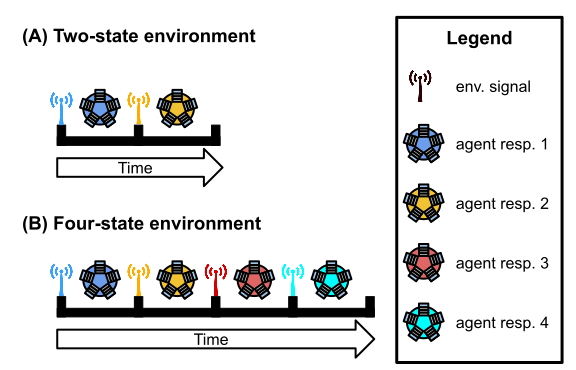
\includegraphics{experiments/2020-11-11-chg-sig/analysis/../../../media/changing-signal-task.png}

Requiring programs to express a distinct instruction in response to each environmental signal represents programs having to perform distinct behaviors.

We afforded programs 128 time steps to express the appropriate response after receiving an environmental signal.
Once the allotted time to respond expires or the program expresses any response, the program's threads of execution are reset, resulting in a loss of all thread-local memory.
\emph{Only} the contents of a program's global memory and each function's regulatory state persist.
The environment then produces the next signal (distinct from all previous signals) to which the program may respond.
A program's fitness is equal to the number of correct responses expressed during evaluation.

We evolved populations of 1000 SignalGP programs to solve the changing-signal task at \(K=16\) (where \(K\) denotes the number of environmental signals).
We evolved populations for \ensuremath{10^{4}} generations or until an program capable of achieving a perfect score during task evaluation (i.e., able to express the appropriate response to each of the \(K\) signals) evolved.

We ran 200 replicate populations (each with a distinct random number seed) of each of the following experimental conditions:

\begin{enumerate}
\def\labelenumi{\arabic{enumi}.}
\tightlist
\item
  a regulation-enabled treatment where programs have access to genetic regulation.
\item
  a regulation-disabled treatment where programs do not have access to genetic regulation.
\end{enumerate}

Note this task does not require programs to shift their response to particular signals over time, and as such, genetic regulation is unnecessary.
Further, because programs experience environmental inputs in a random order, erroneous genetic regulation can manifest as cryptic variation.
For example, non-adaptive down-regulation of a particular response function may be neutral given one sequence of environmental signals, but may be deleterious in another.
\textbf{We expected regulation-enabled SignalGP to exhibit non-adaptive plasticity, potentially resulting in slower adaptation and non-general solutions.}

\hypertarget{analysis-dependencies-4}{%
\section{Analysis Dependencies}\label{analysis-dependencies-4}}

Load all required R libraries.

\begin{Shaded}
\begin{Highlighting}[]
\FunctionTok{library}\NormalTok{(ggplot2)}
\FunctionTok{library}\NormalTok{(tidyverse)}
\FunctionTok{library}\NormalTok{(cowplot)}
\FunctionTok{library}\NormalTok{(viridis)}
\FunctionTok{source}\NormalTok{(}\StringTok{"https://gist.githubusercontent.com/benmarwick/2a1bb0133ff568cbe28d/raw/fb53bd97121f7f9ce947837ef1a4c65a73bffb3f/geom\_flat\_violin.R"}\NormalTok{)}
\end{Highlighting}
\end{Shaded}

These analyses were conducted in the following computing environment:

\begin{Shaded}
\begin{Highlighting}[]
\FunctionTok{print}\NormalTok{(version)}
\end{Highlighting}
\end{Shaded}

\begin{verbatim}
##                _                           
## platform       x86_64-apple-darwin15.6.0   
## arch           x86_64                      
## os             darwin15.6.0                
## system         x86_64, darwin15.6.0        
## status                                     
## major          3                           
## minor          6.2                         
## year           2019                        
## month          12                          
## day            12                          
## svn rev        77560                       
## language       R                           
## version.string R version 3.6.2 (2019-12-12)
## nickname       Dark and Stormy Night
\end{verbatim}

\hypertarget{setup-3}{%
\section{Setup}\label{setup-3}}

Load data, initial data cleanup, configure some global settings.

\begin{Shaded}
\begin{Highlighting}[]
\CommentTok{\# Load data file}
\NormalTok{data\_loc }\OtherTok{\textless{}{-}} \FunctionTok{paste0}\NormalTok{(working\_directory, }\StringTok{"data/max\_fit\_orgs.csv"}\NormalTok{)}
\NormalTok{data }\OtherTok{\textless{}{-}} \FunctionTok{read.csv}\NormalTok{(data\_loc, }\AttributeTok{na.strings=}\StringTok{"NONE"}\NormalTok{)}

\CommentTok{\# Define function to summarize regulation/memory configurations.}
\NormalTok{get\_con }\OtherTok{\textless{}{-}} \ControlFlowTok{function}\NormalTok{(reg, mem) \{}
  \ControlFlowTok{if}\NormalTok{ (reg }\SpecialCharTok{==} \StringTok{"0"} \SpecialCharTok{\&\&}\NormalTok{ mem }\SpecialCharTok{==} \StringTok{"0"}\NormalTok{) \{}
    \FunctionTok{return}\NormalTok{(}\StringTok{"none"}\NormalTok{)}
\NormalTok{  \} }\ControlFlowTok{else} \ControlFlowTok{if}\NormalTok{ (reg }\SpecialCharTok{==} \StringTok{"0"} \SpecialCharTok{\&\&}\NormalTok{ mem}\SpecialCharTok{==}\StringTok{"1"}\NormalTok{) \{}
    \FunctionTok{return}\NormalTok{(}\StringTok{"memory"}\NormalTok{)}
\NormalTok{  \} }\ControlFlowTok{else} \ControlFlowTok{if}\NormalTok{ (reg}\SpecialCharTok{==}\StringTok{"1"} \SpecialCharTok{\&\&}\NormalTok{ mem}\SpecialCharTok{==}\StringTok{"0"}\NormalTok{) \{}
    \FunctionTok{return}\NormalTok{(}\StringTok{"regulation"}\NormalTok{)}
\NormalTok{  \} }\ControlFlowTok{else} \ControlFlowTok{if}\NormalTok{ (reg}\SpecialCharTok{==}\StringTok{"1"} \SpecialCharTok{\&\&}\NormalTok{ mem}\SpecialCharTok{==}\StringTok{"1"}\NormalTok{) \{}
    \FunctionTok{return}\NormalTok{(}\StringTok{"both"}\NormalTok{)}
\NormalTok{  \} }\ControlFlowTok{else}\NormalTok{ \{}
    \FunctionTok{return}\NormalTok{(}\StringTok{"UNKNOWN"}\NormalTok{)}
\NormalTok{  \}}
\NormalTok{\}}

\CommentTok{\# Specify experimental condition for each datum.}
\NormalTok{data}\SpecialCharTok{$}\NormalTok{condition }\OtherTok{\textless{}{-}} \FunctionTok{mapply}\NormalTok{(}
\NormalTok{  get\_con,}
\NormalTok{  data}\SpecialCharTok{$}\NormalTok{USE\_FUNC\_REGULATION,}
\NormalTok{  data}\SpecialCharTok{$}\NormalTok{USE\_GLOBAL\_MEMORY}
\NormalTok{)}

\NormalTok{data}\SpecialCharTok{$}\NormalTok{condition }\OtherTok{\textless{}{-}} \FunctionTok{factor}\NormalTok{(}
\NormalTok{  data}\SpecialCharTok{$}\NormalTok{condition,}
  \AttributeTok{levels=}\FunctionTok{c}\NormalTok{(}\StringTok{"regulation"}\NormalTok{, }\StringTok{"memory"}\NormalTok{, }\StringTok{"none"}\NormalTok{, }\StringTok{"both"}\NormalTok{)}
\NormalTok{)}

\CommentTok{\# For convenience, create a data set with only solutions}
\CommentTok{\# Filter data to include only replicates labeled as solutions}
\NormalTok{sol\_data }\OtherTok{\textless{}{-}} \FunctionTok{filter}\NormalTok{(}
\NormalTok{  data,}
\NormalTok{  solution}\SpecialCharTok{==}\StringTok{"1"}
\NormalTok{)}

\CommentTok{\# A lookup table for task complexities}
\NormalTok{task\_label\_lu }\OtherTok{\textless{}{-}} \FunctionTok{c}\NormalTok{(}
  \StringTok{"2"} \OtherTok{=} \StringTok{"2{-}signal task"}\NormalTok{,}
  \StringTok{"4"} \OtherTok{=} \StringTok{"4{-}signal task"}\NormalTok{,}
  \StringTok{"8"} \OtherTok{=} \StringTok{"8{-}signal task"}\NormalTok{,}
  \StringTok{"16"} \OtherTok{=} \StringTok{"16{-}signal task"}\NormalTok{,}
  \StringTok{"32"} \OtherTok{=}\StringTok{"32{-}signal task"}
\NormalTok{)}

\CommentTok{\# Configure our default graphing theme}
\FunctionTok{theme\_set}\NormalTok{(}\FunctionTok{theme\_cowplot}\NormalTok{())}
\end{Highlighting}
\end{Shaded}

\hypertarget{does-regulation-hinder-the-evolution-of-successful-genotypes}{%
\section{Does regulation hinder the evolution of successful genotypes?}\label{does-regulation-hinder-the-evolution-of-successful-genotypes}}

Here, we look at the number of solutions evolved under regulation-enabled and regulation-disabled conditions.
A program is categorized as a `solution' if it can correctly respond to each of the \(K\) environmental signals \emph{during evaluation}.

\begin{Shaded}
\begin{Highlighting}[]
\CommentTok{\# Graph the number of solutions evolved in each condition, faceted by environmental complexity}
\FunctionTok{ggplot}\NormalTok{( sol\_data, }\FunctionTok{aes}\NormalTok{(}\AttributeTok{x=}\NormalTok{condition, }\AttributeTok{fill=}\NormalTok{condition) ) }\SpecialCharTok{+}
  \FunctionTok{geom\_bar}\NormalTok{() }\SpecialCharTok{+}
  \FunctionTok{geom\_text}\NormalTok{(}
    \AttributeTok{stat=}\StringTok{"count"}\NormalTok{,}
    \AttributeTok{mapping=}\FunctionTok{aes}\NormalTok{(}\AttributeTok{label=}\NormalTok{..count..),}
    \AttributeTok{position=}\FunctionTok{position\_dodge}\NormalTok{(}\FloatTok{0.9}\NormalTok{),}
    \AttributeTok{vjust=}\DecValTok{0}
\NormalTok{  ) }\SpecialCharTok{+}
  \FunctionTok{scale\_x\_discrete}\NormalTok{(}
    \AttributeTok{name=}\StringTok{"Condition"}\NormalTok{,}
    \AttributeTok{breaks=}\FunctionTok{c}\NormalTok{(}\StringTok{"memory"}\NormalTok{,}\StringTok{"both"}\NormalTok{),}
    \AttributeTok{labels=}\FunctionTok{c}\NormalTok{(}\StringTok{"Regulation{-}}\SpecialCharTok{\textbackslash{}n}\StringTok{disabled"}\NormalTok{,}\StringTok{"Regulation{-}}\SpecialCharTok{\textbackslash{}n}\StringTok{enabled"}\NormalTok{)}
\NormalTok{  ) }\SpecialCharTok{+}
  \FunctionTok{ylab}\NormalTok{(}\StringTok{"\# successful replciates (/200)"}\NormalTok{) }\SpecialCharTok{+}
  \FunctionTok{theme}\NormalTok{(}\AttributeTok{legend.position =} \StringTok{"none"}\NormalTok{) }\SpecialCharTok{+}
  \FunctionTok{ggtitle}\NormalTok{(}\StringTok{"Successful replicates"}\NormalTok{)}
\end{Highlighting}
\end{Shaded}

\includegraphics{tag-based-regulation-supplemental_files/figure-latex/unnamed-chunk-89-1.pdf}

Programs capable of achieving a perfect score on the changing-signal task (for a given sequence of environment signals) evolve in all 200 replicates of each condition (i.e., with and without access to genetic regulation).
These programs, however, do not necessarily generalize across all possible sequences of environmental signals.

\hypertarget{does-access-to-regulation-slow-adaptation}{%
\subsection{Does access to regulation slow adaptation?}\label{does-access-to-regulation-slow-adaptation}}

I.e., did successful regulation-enabled programs take longer (more generations) to evolve than those evolved in the regulation-disabled treatment?

\begin{Shaded}
\begin{Highlighting}[]
\FunctionTok{ggplot}\NormalTok{( sol\_data, }\FunctionTok{aes}\NormalTok{(}\AttributeTok{x=}\NormalTok{condition, }\AttributeTok{y=}\NormalTok{update, }\AttributeTok{fill=}\NormalTok{condition) ) }\SpecialCharTok{+}
  \FunctionTok{geom\_flat\_violin}\NormalTok{(}
    \AttributeTok{position =} \FunctionTok{position\_nudge}\NormalTok{(}\AttributeTok{x =}\NormalTok{ .}\DecValTok{2}\NormalTok{, }\AttributeTok{y =} \DecValTok{0}\NormalTok{),}
    \AttributeTok{alpha =}\NormalTok{ .}\DecValTok{8}
\NormalTok{  ) }\SpecialCharTok{+}
  \FunctionTok{geom\_point}\NormalTok{(}
    \FunctionTok{aes}\NormalTok{(}\AttributeTok{y =}\NormalTok{ update, }\AttributeTok{color =}\NormalTok{ condition),}
    \AttributeTok{position =} \FunctionTok{position\_jitter}\NormalTok{(}\AttributeTok{width =}\NormalTok{ .}\DecValTok{15}\NormalTok{),}
    \AttributeTok{size =}\NormalTok{ .}\DecValTok{5}\NormalTok{,}
    \AttributeTok{alpha =} \FloatTok{0.8}
\NormalTok{  ) }\SpecialCharTok{+}
  \FunctionTok{geom\_boxplot}\NormalTok{(}
    \AttributeTok{width =}\NormalTok{ .}\DecValTok{1}\NormalTok{,}
    \AttributeTok{outlier.shape =} \ConstantTok{NA}\NormalTok{,}
    \AttributeTok{alpha =} \FloatTok{0.5}
\NormalTok{  ) }\SpecialCharTok{+}
  \FunctionTok{scale\_x\_discrete}\NormalTok{(}
    \AttributeTok{name=}\StringTok{"Condition"}\NormalTok{,}
    \AttributeTok{breaks=}\FunctionTok{c}\NormalTok{(}\StringTok{"memory"}\NormalTok{, }\StringTok{"both"}\NormalTok{),}
    \AttributeTok{labels=}\FunctionTok{c}\NormalTok{(}\StringTok{"Regulation{-}}\SpecialCharTok{\textbackslash{}n}\StringTok{disabled"}\NormalTok{,}\StringTok{"Regulation{-}}\SpecialCharTok{\textbackslash{}n}\StringTok{enabled"}\NormalTok{)}
\NormalTok{  ) }\SpecialCharTok{+}
  \FunctionTok{scale\_y\_continuous}\NormalTok{(}
    \AttributeTok{name=}\StringTok{"Generation first solution evolved }\SpecialCharTok{\textbackslash{}n}\StringTok{(log scale)"}\NormalTok{,}
\NormalTok{  ) }\SpecialCharTok{+}
  \FunctionTok{guides}\NormalTok{(}\AttributeTok{fill =} \ConstantTok{FALSE}\NormalTok{) }\SpecialCharTok{+}
  \FunctionTok{guides}\NormalTok{(}\AttributeTok{color =} \ConstantTok{FALSE}\NormalTok{)}
\end{Highlighting}
\end{Shaded}

\includegraphics{tag-based-regulation-supplemental_files/figure-latex/unnamed-chunk-90-1.pdf}

\begin{Shaded}
\begin{Highlighting}[]
\FunctionTok{print}\NormalTok{(}\FunctionTok{wilcox.test}\NormalTok{(}\AttributeTok{formula=}\NormalTok{update}\SpecialCharTok{\textasciitilde{}}\NormalTok{condition, }\AttributeTok{data=}\NormalTok{sol\_data, }\AttributeTok{exact=}\ConstantTok{FALSE}\NormalTok{, }\AttributeTok{conf.int=}\ConstantTok{TRUE}\NormalTok{))}
\end{Highlighting}
\end{Shaded}

\begin{verbatim}
## 
##  Wilcoxon rank sum test with continuity correction
## 
## data:  update by condition
## W = 22188, p-value = 0.05845
## alternative hypothesis: true location shift is not equal to 0
## 95 percent confidence interval:
##  -3.860236e-05  1.000000e+01
## sample estimates:
## difference in location 
##               5.000013
\end{verbatim}

The difference in the number of generations before a solution arises is not significantly different.

\hypertarget{do-they-generalize}{%
\subsection{Do they generalize?}\label{do-they-generalize}}

Note that solutions may or may not generalize beyond the sequence of environmental signals on which they achieved a perfect score (and were thus categorized as a `solution').
We re-evaluated each `solution' on a random sample of 5000 sequences of environmental signals to test for generalization.
We deem programs as having successfully generalized only if they responded correctly in all 5000 tests.

To see if regulation is preventing some regulation-enabled solutions from generalizing, we test generalization for regulation-enabled solutions with their regulation faculties knocked out (i.e., regulation instructions replaced with no-operations).

\begin{Shaded}
\begin{Highlighting}[]
\CommentTok{\# Grab count data to make bar plot life easier}
\NormalTok{num\_solutions\_reg }\OtherTok{\textless{}{-}} \FunctionTok{length}\NormalTok{(}\FunctionTok{filter}\NormalTok{(data, condition}\SpecialCharTok{==}\StringTok{"both"} \SpecialCharTok{\&}\NormalTok{ solution}\SpecialCharTok{==}\StringTok{"1"}\NormalTok{)}\SpecialCharTok{$}\NormalTok{SEED)}
\NormalTok{num\_generalize\_reg }\OtherTok{\textless{}{-}} \FunctionTok{length}\NormalTok{(}\FunctionTok{filter}\NormalTok{(data, condition}\SpecialCharTok{==}\StringTok{"both"} \SpecialCharTok{\&}\NormalTok{ all\_solution}\SpecialCharTok{==}\StringTok{"1"}\NormalTok{)}\SpecialCharTok{$}\NormalTok{SEED)}
\NormalTok{num\_generalize\_ko\_reg }\OtherTok{\textless{}{-}} \FunctionTok{length}\NormalTok{(}\FunctionTok{filter}\NormalTok{(data, condition}\SpecialCharTok{==}\StringTok{"both"} \SpecialCharTok{\&}\NormalTok{ all\_solution\_ko\_reg}\SpecialCharTok{==}\StringTok{"1"}\NormalTok{)}\SpecialCharTok{$}\NormalTok{SEED)}

\NormalTok{num\_generalize\_mem }\OtherTok{\textless{}{-}} \FunctionTok{length}\NormalTok{(}\FunctionTok{filter}\NormalTok{(data, condition}\SpecialCharTok{==}\StringTok{"memory"} \SpecialCharTok{\&}\NormalTok{ all\_solution}\SpecialCharTok{==}\StringTok{"1"}\NormalTok{)}\SpecialCharTok{$}\NormalTok{SEED)}

\NormalTok{sol\_cnts }\OtherTok{\textless{}{-}} \FunctionTok{data.frame}\NormalTok{(}\AttributeTok{x=}\DecValTok{1}\SpecialCharTok{:}\DecValTok{3}\NormalTok{)}
\NormalTok{sol\_cnts}\SpecialCharTok{$}\NormalTok{type }\OtherTok{\textless{}{-}} \FunctionTok{c}\NormalTok{(}\StringTok{"reg\_generalize"}\NormalTok{, }\StringTok{"reg\_generalize\_ko\_reg"}\NormalTok{, }\StringTok{"mem\_generalize"}\NormalTok{)}
\NormalTok{sol\_cnts}\SpecialCharTok{$}\NormalTok{val }\OtherTok{\textless{}{-}} \FunctionTok{c}\NormalTok{(num\_generalize\_reg, num\_generalize\_ko\_reg, num\_generalize\_mem)}

\FunctionTok{ggplot}\NormalTok{( sol\_cnts, }\FunctionTok{aes}\NormalTok{(}\AttributeTok{x=}\NormalTok{type, }\AttributeTok{y=}\NormalTok{val, }\AttributeTok{fill=}\NormalTok{type) ) }\SpecialCharTok{+}
  \FunctionTok{geom\_bar}\NormalTok{(}\AttributeTok{stat=}\StringTok{"identity"}\NormalTok{) }\SpecialCharTok{+}
  \FunctionTok{geom\_text}\NormalTok{(}
    \FunctionTok{aes}\NormalTok{(}\AttributeTok{label=}\NormalTok{val),}
    \AttributeTok{stat=}\StringTok{"identity"}\NormalTok{,}
    \AttributeTok{position=}\FunctionTok{position\_dodge}\NormalTok{(}\FloatTok{0.75}\NormalTok{),}
    \AttributeTok{vjust=}\SpecialCharTok{{-}}\FloatTok{0.01}
\NormalTok{  ) }\SpecialCharTok{+}
  \FunctionTok{scale\_x\_discrete}\NormalTok{(}
    \AttributeTok{name=}\StringTok{"Condition"}\NormalTok{,}
    \AttributeTok{limits=}\FunctionTok{c}\NormalTok{(}
      \StringTok{"mem\_generalize"}\NormalTok{,}
      \StringTok{"reg\_generalize"}\NormalTok{,}
      \StringTok{"reg\_generalize\_ko\_reg"}
\NormalTok{      ),}
    \AttributeTok{labels=}\FunctionTok{c}\NormalTok{(}
      \StringTok{"Regulation{-}}\SpecialCharTok{\textbackslash{}n}\StringTok{disabled"}\NormalTok{,}
      \StringTok{"Regulation{-}}\SpecialCharTok{\textbackslash{}n}\StringTok{enabled"}\NormalTok{,}
      \StringTok{"Regulation{-}}\SpecialCharTok{\textbackslash{}n}\StringTok{enabled}\SpecialCharTok{\textbackslash{}n}\StringTok{(reg. KO)"}
\NormalTok{    )}
\NormalTok{  ) }\SpecialCharTok{+}
  \FunctionTok{scale\_y\_continuous}\NormalTok{(}
    \AttributeTok{name=}\StringTok{"Solutions that generalize"}\NormalTok{,}
    \AttributeTok{limits=}\FunctionTok{c}\NormalTok{(}\DecValTok{0}\NormalTok{, }\DecValTok{210}\NormalTok{),}
    \AttributeTok{breaks=}\FunctionTok{seq}\NormalTok{(}\DecValTok{0}\NormalTok{,}\DecValTok{200}\NormalTok{,}\DecValTok{50}\NormalTok{)}
\NormalTok{  ) }\SpecialCharTok{+}
  \FunctionTok{theme}\NormalTok{(}
    \AttributeTok{legend.position=}\StringTok{"none"}\NormalTok{,}
    \AttributeTok{axis.text.x =} \FunctionTok{element\_text}\NormalTok{(}\AttributeTok{size=}\DecValTok{10}\NormalTok{)}
\NormalTok{  ) }\SpecialCharTok{+}
  \FunctionTok{ggsave}\NormalTok{(}\FunctionTok{paste0}\NormalTok{(working\_directory, }\StringTok{"imgs/chg{-}env{-}16{-}generalization.png"}\NormalTok{), }\AttributeTok{width=}\DecValTok{4}\NormalTok{,}\AttributeTok{height=}\DecValTok{4}\NormalTok{)}
\end{Highlighting}
\end{Shaded}

\includegraphics{tag-based-regulation-supplemental_files/figure-latex/unnamed-chunk-91-1.pdf}

All regulation-disabled programs successfully generalized.

\begin{Shaded}
\begin{Highlighting}[]
\NormalTok{table }\OtherTok{\textless{}{-}} \FunctionTok{matrix}\NormalTok{(}\FunctionTok{c}\NormalTok{(num\_generalize\_reg,}
\NormalTok{                  num\_generalize\_mem,}
                  \DecValTok{200} \SpecialCharTok{{-}}\NormalTok{ num\_generalize\_reg,}
                  \DecValTok{200} \SpecialCharTok{{-}}\NormalTok{ num\_generalize\_mem),}
                \AttributeTok{nrow=}\DecValTok{2}\NormalTok{)}
\FunctionTok{rownames}\NormalTok{(table) }\OtherTok{\textless{}{-}} \FunctionTok{c}\NormalTok{(}\StringTok{"reg{-}augmented"}\NormalTok{, }\StringTok{"reg{-}disabled"}\NormalTok{)}
\FunctionTok{colnames}\NormalTok{(table) }\OtherTok{\textless{}{-}} \FunctionTok{c}\NormalTok{(}\StringTok{"success"}\NormalTok{, }\StringTok{"fail"}\NormalTok{)}
\FunctionTok{print}\NormalTok{(table)}
\end{Highlighting}
\end{Shaded}

\begin{verbatim}
##               success fail
## reg-augmented     182   18
## reg-disabled      200    0
\end{verbatim}

\begin{Shaded}
\begin{Highlighting}[]
\FunctionTok{fisher.test}\NormalTok{(table)}
\end{Highlighting}
\end{Shaded}

\begin{verbatim}
## 
##  Fisher's Exact Test for Count Data
## 
## data:  table
## p-value = 5.113e-06
## alternative hypothesis: true odds ratio is not equal to 1
## 95 percent confidence interval:
##  0.0000000 0.2115509
## sample estimates:
## odds ratio 
##          0
\end{verbatim}

The difference in number of generalizing solutions between regulation-enabled and regulation-disabled conditions is statistically significant (Fisher's exact test).

Moreover, 5 of the 18 non-generalizing programs generalize when we knockout genetic regulation.
Upon close inspection, the other 13 non-general programs relied on genetic regulation to achieve initial success but failed to generalize to arbitrary environment signal sequences.

\hypertarget{boolean-calculator-problem-postfix-notation}{%
\chapter{Boolean calculator problem (postfix notation)}\label{boolean-calculator-problem-postfix-notation}}

Here, we give an overview of the boolean-logic calculator problem, and we provide our data analyses for related experiments.
All of our source code for statistical analyses and data visualizations is embedded in this document.
The raw data can be found on the OSF project associated with this work \citep{Lalejini_Moreno_Ofria_Data_2020}.

\textbf{Please \href{https://github.com/amlalejini/Tag-based-Genetic-Regulation-for-LinearGP/issues}{file an issue or make a pull request on github} to report any mistakes, ask questions, request more explanation, et cetera.}

\hypertarget{overview-4}{%
\section{Overview}\label{overview-4}}

\begin{Shaded}
\begin{Highlighting}[]
\CommentTok{\# Experimental parameters referenced in{-}text all in one convenient place.}
\NormalTok{time\_steps }\OtherTok{\textless{}{-}} \DecValTok{128}
\NormalTok{replicates }\OtherTok{\textless{}{-}} \DecValTok{200}
\NormalTok{population\_size }\OtherTok{\textless{}{-}} \DecValTok{1000}
\NormalTok{generations }\OtherTok{\textless{}{-}} \DecValTok{10000}

\CommentTok{\# Settings for statistical analyses.}
\NormalTok{alpha }\OtherTok{\textless{}{-}} \FloatTok{0.05}

\CommentTok{\# Relative location of data.}
\NormalTok{working\_directory }\OtherTok{\textless{}{-}} \StringTok{"experiments/2020{-}11{-}28{-}bool{-}calc{-}postfix/analysis/"} \CommentTok{\# \textless{}\textless{} For bookdown}
\CommentTok{\# working\_directory \textless{}{-} "./"                                              \# \textless{}\textless{} For local analysis}
\end{Highlighting}
\end{Shaded}

We use a modified version of the Boolean-logic calculator problem to further investigate the potential for our implementation of tag-based regulation to impede adaptive evolution.
Our previous experiments with the Boolean-logic calculator problem provided inputs in prefix notation: the operator (e.g., AND, OR, XOR, etc.) is specified first, followed by the requisite number of numeric operands.
As such, the final input signal does not differentiate which type of computation a program is expected to perform (e.g., AND, OR, XOR, etc.).
This requires programs to adjust their response to the final input signal based on the context provided by the previous two signals, thereby increasing the value of regulation.

We explore whether the calculator problem's context-dependence is driving the benefit of tag-based regulation that we identified in previous experiments.
We can reduce context-dependence of the calculator problem by presenting input sequences in postfix notation.
In postfix notation, programs receive the requisite numeric operand inputs first and the operator input last.
As such, the final signal in an input sequence will always differentiate which bitwise operation should be performed.
Successful programs must store the numeric inputs embedded in operand signals, and then, as in the changing-signal problem, a distinct signal will differentiate which of the response types a program should execute.

\hypertarget{analysis-dependencies-5}{%
\section{Analysis Dependencies}\label{analysis-dependencies-5}}

Load all required R libraries.

\begin{Shaded}
\begin{Highlighting}[]
\FunctionTok{library}\NormalTok{(ggplot2)}
\FunctionTok{library}\NormalTok{(tidyverse)}
\FunctionTok{library}\NormalTok{(cowplot)}
\FunctionTok{library}\NormalTok{(viridis)}
\FunctionTok{library}\NormalTok{(reshape2)}
\FunctionTok{library}\NormalTok{(igraph)}
\FunctionTok{source}\NormalTok{(}\StringTok{"https://gist.githubusercontent.com/benmarwick/2a1bb0133ff568cbe28d/raw/fb53bd97121f7f9ce947837ef1a4c65a73bffb3f/geom\_flat\_violin.R"}\NormalTok{)}
\end{Highlighting}
\end{Shaded}

These analyses were conducted in the following computing environment:

\begin{Shaded}
\begin{Highlighting}[]
\FunctionTok{print}\NormalTok{(version)}
\end{Highlighting}
\end{Shaded}

\begin{verbatim}
##                _                           
## platform       x86_64-apple-darwin15.6.0   
## arch           x86_64                      
## os             darwin15.6.0                
## system         x86_64, darwin15.6.0        
## status                                     
## major          3                           
## minor          6.2                         
## year           2019                        
## month          12                          
## day            12                          
## svn rev        77560                       
## language       R                           
## version.string R version 3.6.2 (2019-12-12)
## nickname       Dark and Stormy Night
\end{verbatim}

\hypertarget{setup-4}{%
\section{Setup}\label{setup-4}}

Load data, initial data cleanup, configure some global settings.

\begin{Shaded}
\begin{Highlighting}[]
\NormalTok{data\_loc }\OtherTok{\textless{}{-}} \FunctionTok{paste0}\NormalTok{(working\_directory, }\StringTok{"data/max\_fit\_orgs.csv"}\NormalTok{)}
\NormalTok{data }\OtherTok{\textless{}{-}} \FunctionTok{read.csv}\NormalTok{(data\_loc, }\AttributeTok{na.strings=}\StringTok{"NONE"}\NormalTok{)}

\CommentTok{\# Specify factors (not all of these matter for this set of runs).}
\NormalTok{data}\SpecialCharTok{$}\NormalTok{matchbin\_thresh }\OtherTok{\textless{}{-}} \FunctionTok{factor}\NormalTok{(}
\NormalTok{  data}\SpecialCharTok{$}\NormalTok{matchbin\_thresh,}
  \AttributeTok{levels=}\FunctionTok{c}\NormalTok{(}\DecValTok{0}\NormalTok{, }\DecValTok{25}\NormalTok{, }\DecValTok{50}\NormalTok{, }\DecValTok{75}\NormalTok{)}
\NormalTok{)}

\NormalTok{data}\SpecialCharTok{$}\NormalTok{TAG\_LEN }\OtherTok{\textless{}{-}} \FunctionTok{factor}\NormalTok{(}
\NormalTok{  data}\SpecialCharTok{$}\NormalTok{TAG\_LEN,}
  \AttributeTok{levels=}\FunctionTok{c}\NormalTok{(}\DecValTok{32}\NormalTok{, }\DecValTok{64}\NormalTok{, }\DecValTok{128}\NormalTok{, }\DecValTok{256}\NormalTok{)}
\NormalTok{)}

\NormalTok{data}\SpecialCharTok{$}\NormalTok{notation }\OtherTok{\textless{}{-}} \FunctionTok{factor}\NormalTok{(}
\NormalTok{  data}\SpecialCharTok{$}\NormalTok{notation,}
  \AttributeTok{levels=}\FunctionTok{c}\NormalTok{(}\StringTok{"prefix"}\NormalTok{, }\StringTok{"postfix"}\NormalTok{)}
\NormalTok{)}

\CommentTok{\# Define function to summarize regulation/memory configurations.}
\NormalTok{get\_con }\OtherTok{\textless{}{-}} \ControlFlowTok{function}\NormalTok{(reg, mem) \{}
  \ControlFlowTok{if}\NormalTok{ (reg }\SpecialCharTok{==} \StringTok{"0"} \SpecialCharTok{\&\&}\NormalTok{ mem }\SpecialCharTok{==} \StringTok{"0"}\NormalTok{) \{}
    \FunctionTok{return}\NormalTok{(}\StringTok{"none"}\NormalTok{)}
\NormalTok{  \} }\ControlFlowTok{else} \ControlFlowTok{if}\NormalTok{ (reg }\SpecialCharTok{==} \StringTok{"0"} \SpecialCharTok{\&\&}\NormalTok{ mem}\SpecialCharTok{==}\StringTok{"1"}\NormalTok{) \{}
    \FunctionTok{return}\NormalTok{(}\StringTok{"memory"}\NormalTok{)}
\NormalTok{  \} }\ControlFlowTok{else} \ControlFlowTok{if}\NormalTok{ (reg}\SpecialCharTok{==}\StringTok{"1"} \SpecialCharTok{\&\&}\NormalTok{ mem}\SpecialCharTok{==}\StringTok{"0"}\NormalTok{) \{}
    \FunctionTok{return}\NormalTok{(}\StringTok{"regulation"}\NormalTok{)}
\NormalTok{  \} }\ControlFlowTok{else} \ControlFlowTok{if}\NormalTok{ (reg}\SpecialCharTok{==}\StringTok{"1"} \SpecialCharTok{\&\&}\NormalTok{ mem}\SpecialCharTok{==}\StringTok{"1"}\NormalTok{) \{}
    \FunctionTok{return}\NormalTok{(}\StringTok{"both"}\NormalTok{)}
\NormalTok{  \} }\ControlFlowTok{else}\NormalTok{ \{}
    \FunctionTok{return}\NormalTok{(}\StringTok{"UNKNOWN"}\NormalTok{)}
\NormalTok{  \}}
\NormalTok{\}}

\CommentTok{\# Specify experimental condition for each datum.}
\NormalTok{data}\SpecialCharTok{$}\NormalTok{condition }\OtherTok{\textless{}{-}} \FunctionTok{mapply}\NormalTok{(}
\NormalTok{  get\_con,}
\NormalTok{  data}\SpecialCharTok{$}\NormalTok{USE\_FUNC\_REGULATION,}
\NormalTok{  data}\SpecialCharTok{$}\NormalTok{USE\_GLOBAL\_MEMORY}
\NormalTok{)}

\NormalTok{data}\SpecialCharTok{$}\NormalTok{condition }\OtherTok{\textless{}{-}} \FunctionTok{factor}\NormalTok{(}
\NormalTok{  data}\SpecialCharTok{$}\NormalTok{condition,}
  \AttributeTok{levels=}\FunctionTok{c}\NormalTok{(}\StringTok{"regulation"}\NormalTok{, }\StringTok{"memory"}\NormalTok{, }\StringTok{"none"}\NormalTok{, }\StringTok{"both"}\NormalTok{)}
\NormalTok{)}

\CommentTok{\# Given knockout info, what strategy does a program use?}
\NormalTok{get\_strategy }\OtherTok{\textless{}{-}} \ControlFlowTok{function}\NormalTok{(use\_reg, use\_mem) \{}
  \ControlFlowTok{if}\NormalTok{ (use\_reg}\SpecialCharTok{==}\StringTok{"0"} \SpecialCharTok{\&\&}\NormalTok{ use\_mem}\SpecialCharTok{==}\StringTok{"0"}\NormalTok{) \{}
    \FunctionTok{return}\NormalTok{(}\StringTok{"use neither"}\NormalTok{)}
\NormalTok{  \} }\ControlFlowTok{else} \ControlFlowTok{if}\NormalTok{ (use\_reg}\SpecialCharTok{==}\StringTok{"0"} \SpecialCharTok{\&\&}\NormalTok{ use\_mem}\SpecialCharTok{==}\StringTok{"1"}\NormalTok{) \{}
    \FunctionTok{return}\NormalTok{(}\StringTok{"use memory"}\NormalTok{)}
\NormalTok{  \} }\ControlFlowTok{else} \ControlFlowTok{if}\NormalTok{ (use\_reg}\SpecialCharTok{==}\StringTok{"1"} \SpecialCharTok{\&\&}\NormalTok{ use\_mem}\SpecialCharTok{==}\StringTok{"0"}\NormalTok{) \{}
    \FunctionTok{return}\NormalTok{(}\StringTok{"use regulation"}\NormalTok{)}
\NormalTok{  \} }\ControlFlowTok{else} \ControlFlowTok{if}\NormalTok{ (use\_reg}\SpecialCharTok{==}\StringTok{"1"} \SpecialCharTok{\&\&}\NormalTok{ use\_mem}\SpecialCharTok{==}\StringTok{"1"}\NormalTok{) \{}
    \FunctionTok{return}\NormalTok{(}\StringTok{"use both"}\NormalTok{)}
\NormalTok{  \} }\ControlFlowTok{else}\NormalTok{ \{}
    \FunctionTok{return}\NormalTok{(}\StringTok{"UNKNOWN"}\NormalTok{)}
\NormalTok{  \}}
\NormalTok{\}}

\CommentTok{\# Specify experimental conditions (to make labeling easier).}
\NormalTok{data}\SpecialCharTok{$}\NormalTok{strategy }\OtherTok{\textless{}{-}} \FunctionTok{mapply}\NormalTok{(}
\NormalTok{  get\_strategy,}
\NormalTok{  data}\SpecialCharTok{$}\NormalTok{relies\_on\_regulation,}
\NormalTok{  data}\SpecialCharTok{$}\NormalTok{relies\_on\_global\_memory}
\NormalTok{)}

\NormalTok{data}\SpecialCharTok{$}\NormalTok{strategy }\OtherTok{\textless{}{-}} \FunctionTok{factor}\NormalTok{(}
\NormalTok{  data}\SpecialCharTok{$}\NormalTok{strategy,}
  \AttributeTok{levels=}\FunctionTok{c}\NormalTok{(}
    \StringTok{"use regulation"}\NormalTok{,}
    \StringTok{"use memory"}\NormalTok{,}
    \StringTok{"use neither"}\NormalTok{,}
    \StringTok{"use both"}
\NormalTok{  )}
\NormalTok{)}

\CommentTok{\# Filter data to include only replicates labeled as solutions}
\NormalTok{sol\_data }\OtherTok{\textless{}{-}} \FunctionTok{filter}\NormalTok{(data, solution}\SpecialCharTok{==}\StringTok{"1"}\NormalTok{)}

\DocumentationTok{\#\#\#\#\#\#\# Load instruction execution data \#\#\#\#\#\#\#}
\NormalTok{inst\_exec\_data }\OtherTok{\textless{}{-}} \FunctionTok{read.csv}\NormalTok{(}\FunctionTok{paste0}\NormalTok{(working\_directory, }\StringTok{"data/exec\_trace\_summary.csv"}\NormalTok{), }\AttributeTok{na.strings=}\StringTok{"NA"}\NormalTok{)}

\NormalTok{inst\_exec\_data}\SpecialCharTok{$}\NormalTok{condition }\OtherTok{\textless{}{-}} \FunctionTok{mapply}\NormalTok{(}
\NormalTok{  get\_con,}
\NormalTok{  inst\_exec\_data}\SpecialCharTok{$}\NormalTok{USE\_FUNC\_REGULATION,}
\NormalTok{  inst\_exec\_data}\SpecialCharTok{$}\NormalTok{USE\_GLOBAL\_MEMORY}
\NormalTok{)}

\NormalTok{inst\_exec\_data}\SpecialCharTok{$}\NormalTok{condition }\OtherTok{\textless{}{-}} \FunctionTok{factor}\NormalTok{(}
\NormalTok{  inst\_exec\_data}\SpecialCharTok{$}\NormalTok{condition,}
  \AttributeTok{levels=}\FunctionTok{c}\NormalTok{(}\StringTok{"regulation"}\NormalTok{, }\StringTok{"memory"}\NormalTok{, }\StringTok{"none"}\NormalTok{, }\StringTok{"both"}\NormalTok{)}
\NormalTok{)}

\NormalTok{inst\_exec\_data}\SpecialCharTok{$}\NormalTok{notation }\OtherTok{\textless{}{-}} \FunctionTok{factor}\NormalTok{(}
\NormalTok{  inst\_exec\_data}\SpecialCharTok{$}\NormalTok{notation,}
  \AttributeTok{levels=}\FunctionTok{c}\NormalTok{(}\StringTok{"prefix"}\NormalTok{, }\StringTok{"postfix"}\NormalTok{)}
\NormalTok{)}

\DocumentationTok{\#\#\#\#\#\#\# Load network data \#\#\#\#\#\#\#}
\NormalTok{reg\_network\_data }\OtherTok{\textless{}{-}} \FunctionTok{read.csv}\NormalTok{(}\FunctionTok{paste0}\NormalTok{(working\_directory, }\StringTok{"data/reg\_graphs\_summary.csv"}\NormalTok{), }\AttributeTok{na.strings=}\StringTok{"NA"}\NormalTok{)}
\NormalTok{reg\_network\_data }\OtherTok{\textless{}{-}} \FunctionTok{filter}\NormalTok{(reg\_network\_data, run\_id }\SpecialCharTok{\%in\%}\NormalTok{ data}\SpecialCharTok{$}\NormalTok{SEED)}

\NormalTok{get\_notation }\OtherTok{\textless{}{-}} \ControlFlowTok{function}\NormalTok{(seed) \{}
  \FunctionTok{return}\NormalTok{(}\FunctionTok{filter}\NormalTok{(data, SEED}\SpecialCharTok{==}\NormalTok{seed)}\SpecialCharTok{$}\NormalTok{notation)}
\NormalTok{\}}

\NormalTok{reg\_network\_data}\SpecialCharTok{$}\NormalTok{notation }\OtherTok{\textless{}{-}} \FunctionTok{mapply}\NormalTok{(}
\NormalTok{  get\_notation,}
\NormalTok{  reg\_network\_data}\SpecialCharTok{$}\NormalTok{run\_id}
\NormalTok{)}

\NormalTok{reg\_network\_data}\SpecialCharTok{$}\NormalTok{notation }\OtherTok{\textless{}{-}} \FunctionTok{factor}\NormalTok{(}
\NormalTok{  reg\_network\_data}\SpecialCharTok{$}\NormalTok{notation,}
  \AttributeTok{levels=}\FunctionTok{c}\NormalTok{(}\StringTok{"prefix"}\NormalTok{, }\StringTok{"postfix"}\NormalTok{)}
\NormalTok{)}

\DocumentationTok{\#\#\#\#\#\#\# misc \#\#\#\#\#\#\#}
\CommentTok{\# Configure our default graphing theme}
\FunctionTok{theme\_set}\NormalTok{(}\FunctionTok{theme\_cowplot}\NormalTok{())}
\end{Highlighting}
\end{Shaded}

\hypertarget{problem-solving-success-3}{%
\section{Problem-solving success}\label{problem-solving-success-3}}

The number of successful replicates by condition:

\begin{Shaded}
\begin{Highlighting}[]
\CommentTok{\# Graph the number of solutions evolved in each condition, faceted by environmental complexity}
\FunctionTok{ggplot}\NormalTok{(sol\_data, }\FunctionTok{aes}\NormalTok{(}\AttributeTok{x=}\NormalTok{condition, }\AttributeTok{fill=}\NormalTok{condition)) }\SpecialCharTok{+}
  \FunctionTok{geom\_bar}\NormalTok{() }\SpecialCharTok{+}
  \FunctionTok{geom\_text}\NormalTok{(}
    \AttributeTok{stat=}\StringTok{"count"}\NormalTok{,}
    \AttributeTok{mapping=}\FunctionTok{aes}\NormalTok{(}\AttributeTok{label=}\NormalTok{..count..),}
    \AttributeTok{position=}\FunctionTok{position\_dodge}\NormalTok{(}\FloatTok{0.9}\NormalTok{),}
    \AttributeTok{vjust=}\DecValTok{0}
\NormalTok{  ) }\SpecialCharTok{+}
  \FunctionTok{scale\_x\_discrete}\NormalTok{(}
    \AttributeTok{name=}\StringTok{"Condition"}\NormalTok{,}
    \AttributeTok{breaks=}\FunctionTok{c}\NormalTok{(}\StringTok{"memory"}\NormalTok{,}\StringTok{"both"}\NormalTok{),}
    \AttributeTok{labels=}\FunctionTok{c}\NormalTok{(}\StringTok{"Regulation{-}}\SpecialCharTok{\textbackslash{}n}\StringTok{disabled"}\NormalTok{, }\StringTok{"Regulation{-}}\SpecialCharTok{\textbackslash{}n}\StringTok{enabled"}\NormalTok{)}
\NormalTok{  ) }\SpecialCharTok{+}
  \FunctionTok{ylab}\NormalTok{(}\StringTok{"Successful replciates"}\NormalTok{) }\SpecialCharTok{+}
  \FunctionTok{ylim}\NormalTok{(}\DecValTok{0}\NormalTok{, }\DecValTok{200}\NormalTok{) }\SpecialCharTok{+}
  \FunctionTok{theme}\NormalTok{(}\AttributeTok{legend.position =} \StringTok{"none"}\NormalTok{) }\SpecialCharTok{+}
  \FunctionTok{ggsave}\NormalTok{(}
    \FunctionTok{paste0}\NormalTok{(working\_directory, }\StringTok{"imgs/boolean{-}calc{-}postfix{-}solution{-}counts.pdf"}\NormalTok{),}
    \AttributeTok{width=}\DecValTok{4}\NormalTok{,}
    \AttributeTok{height=}\DecValTok{4}
\NormalTok{  )}
\end{Highlighting}
\end{Shaded}

\includegraphics{tag-based-regulation-supplemental_files/figure-latex/unnamed-chunk-97-1.pdf}

Test for significance using Fisher's exact test.

\begin{Shaded}
\begin{Highlighting}[]
\CommentTok{\# Extract successes/fails for each condition.}
\NormalTok{reg\_disabled\_success\_cnt }\OtherTok{\textless{}{-}} \FunctionTok{nrow}\NormalTok{(}\FunctionTok{filter}\NormalTok{(sol\_data, solution}\SpecialCharTok{==}\StringTok{"1"} \SpecialCharTok{\&}\NormalTok{ condition}\SpecialCharTok{==}\StringTok{"memory"}\NormalTok{))}
\NormalTok{reg\_disabled\_fail\_cnt }\OtherTok{\textless{}{-}}\NormalTok{ replicates }\SpecialCharTok{{-}}\NormalTok{ reg\_disabled\_success\_cnt}

\NormalTok{reg\_enabled\_success\_cnt }\OtherTok{\textless{}{-}} \FunctionTok{nrow}\NormalTok{(}\FunctionTok{filter}\NormalTok{(sol\_data, solution}\SpecialCharTok{==}\StringTok{"1"} \SpecialCharTok{\&}\NormalTok{ condition}\SpecialCharTok{==}\StringTok{"both"}\NormalTok{))}
\NormalTok{reg\_enabled\_fail\_cnt }\OtherTok{\textless{}{-}}\NormalTok{ replicates }\SpecialCharTok{{-}}\NormalTok{ reg\_enabled\_success\_cnt}

\CommentTok{\# Regulation{-}disabled vs regulation{-}enabled}
\NormalTok{perf\_table }\OtherTok{\textless{}{-}} \FunctionTok{matrix}\NormalTok{(}
  \FunctionTok{c}\NormalTok{(}
\NormalTok{    reg\_enabled\_success\_cnt,}
\NormalTok{    reg\_disabled\_success\_cnt,}
\NormalTok{    reg\_enabled\_fail\_cnt,}
\NormalTok{    reg\_disabled\_fail\_cnt}
\NormalTok{    ),}
    \AttributeTok{nrow=}\DecValTok{2}
\NormalTok{)}

\FunctionTok{rownames}\NormalTok{(perf\_table) }\OtherTok{\textless{}{-}} \FunctionTok{c}\NormalTok{(}\StringTok{"reg{-}enabled"}\NormalTok{, }\StringTok{"reg{-}disabled"}\NormalTok{)}
\FunctionTok{colnames}\NormalTok{(perf\_table) }\OtherTok{\textless{}{-}} \FunctionTok{c}\NormalTok{(}\StringTok{"success"}\NormalTok{, }\StringTok{"fail"}\NormalTok{)}

\FunctionTok{print}\NormalTok{(perf\_table)}
\end{Highlighting}
\end{Shaded}

\begin{verbatim}
##              success fail
## reg-enabled      120   80
## reg-disabled     151   49
\end{verbatim}

\begin{Shaded}
\begin{Highlighting}[]
\FunctionTok{print}\NormalTok{(}\FunctionTok{fisher.test}\NormalTok{(perf\_table))}
\end{Highlighting}
\end{Shaded}

\begin{verbatim}
## 
##  Fisher's Exact Test for Count Data
## 
## data:  perf_table
## p-value = 0.001286
## alternative hypothesis: true odds ratio is not equal to 1
## 95 percent confidence interval:
##  0.3093253 0.7635173
## sample estimates:
## odds ratio 
##  0.4876392
\end{verbatim}

\hypertarget{how-many-generations-elapse-before-solutions-evolve-3}{%
\section{How many generations elapse before solutions evolve?}\label{how-many-generations-elapse-before-solutions-evolve-3}}

\begin{Shaded}
\begin{Highlighting}[]
\NormalTok{unfinished\_data }\OtherTok{\textless{}{-}} \FunctionTok{filter}\NormalTok{(data, solution}\SpecialCharTok{==}\StringTok{"0"}\NormalTok{)}
\NormalTok{unfinished\_data}\SpecialCharTok{$}\NormalTok{graph\_update }\OtherTok{\textless{}{-}} \DecValTok{12500}

\FunctionTok{ggplot}\NormalTok{( ) }\SpecialCharTok{+}
  \FunctionTok{geom\_flat\_violin}\NormalTok{(}
    \AttributeTok{data =}\NormalTok{ sol\_data,}
    \AttributeTok{mapping =} \FunctionTok{aes}\NormalTok{(}\AttributeTok{x=}\NormalTok{condition, }\AttributeTok{y=}\NormalTok{update, }\AttributeTok{fill=}\NormalTok{condition),}
    \AttributeTok{position =} \FunctionTok{position\_nudge}\NormalTok{(}\AttributeTok{x =}\NormalTok{ .}\DecValTok{2}\NormalTok{, }\AttributeTok{y =} \DecValTok{0}\NormalTok{),}
    \AttributeTok{alpha =}\NormalTok{ .}\DecValTok{8}
\NormalTok{  ) }\SpecialCharTok{+}
  \FunctionTok{geom\_point}\NormalTok{(}
    \AttributeTok{data =}\NormalTok{ sol\_data,}
    \FunctionTok{aes}\NormalTok{(}\AttributeTok{x=}\NormalTok{condition, }\AttributeTok{y=}\NormalTok{update, }\AttributeTok{color=}\NormalTok{condition),}
    \AttributeTok{position =} \FunctionTok{position\_jitter}\NormalTok{(}\AttributeTok{width =}\NormalTok{ .}\DecValTok{15}\NormalTok{),}
    \AttributeTok{size =}\NormalTok{ .}\DecValTok{5}\NormalTok{,}
    \AttributeTok{alpha =} \FloatTok{0.8}
\NormalTok{  ) }\SpecialCharTok{+}
  \FunctionTok{geom\_point}\NormalTok{(}
    \AttributeTok{data =}\NormalTok{ unfinished\_data,}
    \AttributeTok{mapping=}\FunctionTok{aes}\NormalTok{(}\AttributeTok{x=}\NormalTok{condition, }\AttributeTok{y=}\NormalTok{graph\_update),}
    \AttributeTok{color=}\StringTok{"gray"}\NormalTok{,}
    \AttributeTok{position =} \FunctionTok{position\_jitter}\NormalTok{(}\AttributeTok{width =}\NormalTok{ .}\DecValTok{15}\NormalTok{, }\AttributeTok{height=}\DecValTok{500}\NormalTok{),}
    \AttributeTok{size =}\NormalTok{ .}\DecValTok{5}\NormalTok{,}
    \AttributeTok{alpha =} \FloatTok{0.8}
\NormalTok{  ) }\SpecialCharTok{+}
  \FunctionTok{geom\_boxplot}\NormalTok{(}
    \AttributeTok{data =}\NormalTok{ sol\_data,}
    \AttributeTok{mapping =} \FunctionTok{aes}\NormalTok{(}\AttributeTok{x=}\NormalTok{condition, }\AttributeTok{y=}\NormalTok{update, }\AttributeTok{fill=}\NormalTok{condition),}
    \AttributeTok{width =}\NormalTok{ .}\DecValTok{1}\NormalTok{,}
    \AttributeTok{outlier.shape =} \ConstantTok{NA}\NormalTok{,}
    \AttributeTok{alpha =} \FloatTok{0.5}
\NormalTok{  ) }\SpecialCharTok{+}
  \FunctionTok{scale\_x\_discrete}\NormalTok{(}
    \AttributeTok{name=}\StringTok{"Condition"}\NormalTok{,}
    \AttributeTok{breaks=}\FunctionTok{c}\NormalTok{(}\StringTok{"memory"}\NormalTok{, }\StringTok{"both"}\NormalTok{),}
    \AttributeTok{labels=}\FunctionTok{c}\NormalTok{(}\StringTok{"Regulation{-}}\SpecialCharTok{\textbackslash{}n}\StringTok{disabled"}\NormalTok{, }\StringTok{"Regulation{-}}\SpecialCharTok{\textbackslash{}n}\StringTok{enabled"}\NormalTok{)}
\NormalTok{  ) }\SpecialCharTok{+}
  \FunctionTok{scale\_y\_continuous}\NormalTok{(}
    \AttributeTok{name=}\StringTok{"Generation first solution evolved"}\NormalTok{,}
    \AttributeTok{limits=}\FunctionTok{c}\NormalTok{(}\DecValTok{0}\NormalTok{, }\DecValTok{13000}\NormalTok{),}
    \AttributeTok{breaks=}\FunctionTok{c}\NormalTok{(}\DecValTok{0}\NormalTok{, }\DecValTok{2500}\NormalTok{, }\DecValTok{5000}\NormalTok{, }\DecValTok{7500}\NormalTok{, }\DecValTok{10000}\NormalTok{, }\DecValTok{12500}\NormalTok{),}
    \AttributeTok{labels=}\FunctionTok{c}\NormalTok{(}\StringTok{"0"}\NormalTok{, }\StringTok{"2500"}\NormalTok{, }\StringTok{"5000"}\NormalTok{, }\StringTok{"7500"}\NormalTok{, }\StringTok{"10000"}\NormalTok{, }\StringTok{"Unsolved"}\NormalTok{)}
\NormalTok{  ) }\SpecialCharTok{+}
  \CommentTok{\# coord\_flip() +}
  \FunctionTok{guides}\NormalTok{(}\AttributeTok{fill =} \ConstantTok{FALSE}\NormalTok{) }\SpecialCharTok{+}
  \FunctionTok{guides}\NormalTok{(}\AttributeTok{color =} \ConstantTok{FALSE}\NormalTok{) }\SpecialCharTok{+}
  \FunctionTok{ggsave}\NormalTok{(}
    \FunctionTok{paste0}\NormalTok{(working\_directory, }\StringTok{"imgs/boolean{-}calc{-}postfix{-}solve{-}time{-}cloud.pdf"}\NormalTok{),}
    \AttributeTok{width=}\DecValTok{4}\NormalTok{,}
    \AttributeTok{height=}\DecValTok{4}
\NormalTok{  )}
\end{Highlighting}
\end{Shaded}

\includegraphics{tag-based-regulation-supplemental_files/figure-latex/unnamed-chunk-99-1.pdf}

Test for statistical difference between conditions using a Wilcoxon rank sum test.

\begin{Shaded}
\begin{Highlighting}[]
\FunctionTok{print}\NormalTok{(}\FunctionTok{wilcox.test}\NormalTok{(}\AttributeTok{formula=}\NormalTok{update}\SpecialCharTok{\textasciitilde{}}\NormalTok{condition, }\AttributeTok{data=}\NormalTok{sol\_data, }\AttributeTok{exact=}\ConstantTok{FALSE}\NormalTok{, }\AttributeTok{conf.int=}\ConstantTok{TRUE}\NormalTok{))}
\end{Highlighting}
\end{Shaded}

\begin{verbatim}
## 
##  Wilcoxon rank sum test with continuity correction
## 
## data:  update by condition
## W = 7175.5, p-value = 0.003285
## alternative hypothesis: true location shift is not equal to 0
## 95 percent confidence interval:
##  -1422  -310
## sample estimates:
## difference in location 
##                   -872
\end{verbatim}

\hypertarget{evolved-strategies-2}{%
\section{Evolved strategies}\label{evolved-strategies-2}}

\hypertarget{program-length-3}{%
\subsection{Program length}\label{program-length-3}}

How long (i.e., total number of instructions) are solutions?

\begin{Shaded}
\begin{Highlighting}[]
\FunctionTok{ggplot}\NormalTok{( sol\_data, }\FunctionTok{aes}\NormalTok{(}\AttributeTok{x=}\NormalTok{condition, }\AttributeTok{y=}\NormalTok{num\_instructions, }\AttributeTok{color=}\NormalTok{condition) ) }\SpecialCharTok{+}
  \FunctionTok{geom\_boxplot}\NormalTok{() }\SpecialCharTok{+}
  \FunctionTok{geom\_jitter}\NormalTok{(}\AttributeTok{alpha=}\FloatTok{0.2}\NormalTok{) }\SpecialCharTok{+}
  \FunctionTok{ylab}\NormalTok{(}\StringTok{"Number of instructions in genome"}\NormalTok{) }\SpecialCharTok{+}
  \FunctionTok{scale\_color\_discrete}\NormalTok{(}
    \AttributeTok{name=}\StringTok{"Condition"}\NormalTok{,}
    \AttributeTok{breaks=}\FunctionTok{c}\NormalTok{(}\StringTok{"memory"}\NormalTok{, }\StringTok{"both"}\NormalTok{),}
    \AttributeTok{labels=}\FunctionTok{c}\NormalTok{(}\StringTok{"Regulation{-}disabled (D)"}\NormalTok{, }\StringTok{"Regulation{-}enabled (E)"}\NormalTok{)}
\NormalTok{  ) }\SpecialCharTok{+}
  \FunctionTok{scale\_x\_discrete}\NormalTok{(}
    \AttributeTok{name=}\StringTok{"Condition"}\NormalTok{,}
    \AttributeTok{breaks=}\FunctionTok{c}\NormalTok{(}\StringTok{"memory"}\NormalTok{, }\StringTok{"both"}\NormalTok{),}
    \AttributeTok{labels=}\FunctionTok{c}\NormalTok{(}\StringTok{"D"}\NormalTok{, }\StringTok{"E"}\NormalTok{)}
\NormalTok{  ) }\SpecialCharTok{+}
  \FunctionTok{theme}\NormalTok{(}
    \AttributeTok{legend.position=}\StringTok{"bottom"}\NormalTok{,}
    \AttributeTok{axis.title.x=}\FunctionTok{element\_blank}\NormalTok{()}
\NormalTok{  )}
\end{Highlighting}
\end{Shaded}

\includegraphics{tag-based-regulation-supplemental_files/figure-latex/unnamed-chunk-101-1.pdf}

\hypertarget{what-mechanisms-do-programs-rely-on-to-adjust-responses-to-signals-over-time-2}{%
\subsection{What mechanisms do programs rely on to adjust responses to signals over time?}\label{what-mechanisms-do-programs-rely-on-to-adjust-responses-to-signals-over-time-2}}

We used indpendent knockouts of tag-based genetic regulation and global memory buffer access to investigate the mechanisms underpinning successful programs.

\begin{Shaded}
\begin{Highlighting}[]
\FunctionTok{ggplot}\NormalTok{( sol\_data, }\AttributeTok{mapping=}\FunctionTok{aes}\NormalTok{(}\AttributeTok{x=}\NormalTok{condition, }\AttributeTok{fill=}\NormalTok{strategy) ) }\SpecialCharTok{+}
  \FunctionTok{geom\_bar}\NormalTok{(}
    \AttributeTok{position=}\StringTok{"fill"}\NormalTok{,}
    \AttributeTok{stat=}\StringTok{"count"}
\NormalTok{  ) }\SpecialCharTok{+}
  \FunctionTok{geom\_text}\NormalTok{(}
    \AttributeTok{stat=}\StringTok{\textquotesingle{}count\textquotesingle{}}\NormalTok{,}
    \AttributeTok{mapping=}\FunctionTok{aes}\NormalTok{(}\AttributeTok{label=}\NormalTok{..count..),}
    \AttributeTok{position=}\FunctionTok{position\_fill}\NormalTok{(}\AttributeTok{vjust=}\FloatTok{0.05}\NormalTok{)}
\NormalTok{  ) }\SpecialCharTok{+}
  \FunctionTok{ylab}\NormalTok{(}\StringTok{"\% of Solutions"}\NormalTok{) }\SpecialCharTok{+}
  \FunctionTok{scale\_fill\_discrete}\NormalTok{(}
    \AttributeTok{name=}\StringTok{"Strategy:"}\NormalTok{,}
    \AttributeTok{breaks=}\FunctionTok{c}\NormalTok{(}
      \StringTok{"use regulation"}\NormalTok{,}
      \StringTok{"use memory"}\NormalTok{,}
      \StringTok{"use neither"}\NormalTok{,}
      \StringTok{"use both"}
\NormalTok{    ),}
    \AttributeTok{labels=}\FunctionTok{c}\NormalTok{(}
      \StringTok{"Use regulation (only)"}\NormalTok{,}
      \StringTok{"Use global memory (only)"}\NormalTok{,}
      \StringTok{"Use neither"}\NormalTok{,}
      \StringTok{"Use both"}
\NormalTok{    )}
\NormalTok{  ) }\SpecialCharTok{+}
  \FunctionTok{scale\_x\_discrete}\NormalTok{(}
    \AttributeTok{name=}\StringTok{"Condition"}\NormalTok{,}
    \AttributeTok{breaks=}\FunctionTok{c}\NormalTok{(}\StringTok{"memory"}\NormalTok{, }\StringTok{"both"}\NormalTok{),}
    \AttributeTok{labels=}\FunctionTok{c}\NormalTok{(}\StringTok{"Regulation{-}}\SpecialCharTok{\textbackslash{}n}\StringTok{disabled"}\NormalTok{, }\StringTok{"Regulation{-}}\SpecialCharTok{\textbackslash{}n}\StringTok{enabled"}\NormalTok{)}
\NormalTok{  ) }\SpecialCharTok{+}
  \FunctionTok{theme}\NormalTok{(}\AttributeTok{legend.position =} \StringTok{"bottom"}\NormalTok{)}
\end{Highlighting}
\end{Shaded}

\includegraphics{tag-based-regulation-supplemental_files/figure-latex/unnamed-chunk-102-1.pdf}

\hypertarget{gene-regulatory-networks-2}{%
\subsection{Gene regulatory networks}\label{gene-regulatory-networks-2}}

Looking only at successful programs that rely on regulation. At a glance, what do gene regulatory networks look like?

First, the total edges found in networks:

\begin{Shaded}
\begin{Highlighting}[]
\NormalTok{relies\_on\_reg }\OtherTok{\textless{}{-}} \FunctionTok{filter}\NormalTok{(}
\NormalTok{  sol\_data,}
\NormalTok{  relies\_on\_regulation}\SpecialCharTok{==}\StringTok{"1"}
\NormalTok{)}\SpecialCharTok{$}\NormalTok{SEED}

\FunctionTok{ggplot}\NormalTok{( }\FunctionTok{filter}\NormalTok{(reg\_network\_data, run\_id }\SpecialCharTok{\%in\%}\NormalTok{ relies\_on\_reg), }\FunctionTok{aes}\NormalTok{(}\AttributeTok{x=}\NormalTok{notation, }\AttributeTok{y=}\NormalTok{edge\_cnt) ) }\SpecialCharTok{+}
  \FunctionTok{geom\_boxplot}\NormalTok{() }\SpecialCharTok{+}
  \FunctionTok{geom\_jitter}\NormalTok{(}\AttributeTok{alpha=}\FloatTok{0.1}\NormalTok{) }\SpecialCharTok{+}
  \FunctionTok{xlab}\NormalTok{(}\StringTok{"Notation"}\NormalTok{) }\SpecialCharTok{+}
  \FunctionTok{ylab}\NormalTok{(}\StringTok{"\# Edges"}\NormalTok{) }\SpecialCharTok{+}
  \FunctionTok{theme}\NormalTok{(}
    \AttributeTok{legend.position=}\StringTok{"bottom"}\NormalTok{,}
    \AttributeTok{legend.text=}\FunctionTok{element\_text}\NormalTok{(}\AttributeTok{size=}\DecValTok{9}\NormalTok{),}
    \AttributeTok{legend.title=}\FunctionTok{element\_text}\NormalTok{(}\AttributeTok{size=}\DecValTok{10}\NormalTok{),}
    \AttributeTok{axis.title.x=}\FunctionTok{element\_text}\NormalTok{(}\AttributeTok{size=}\DecValTok{12}\NormalTok{)}
\NormalTok{  ) }\SpecialCharTok{+}
  \FunctionTok{ggsave}\NormalTok{(}
    \FunctionTok{paste0}\NormalTok{(working\_directory, }\StringTok{"imgs/boolean{-}calc{-}postfix{-}regulation{-}edges.png"}\NormalTok{),}
    \AttributeTok{width=}\DecValTok{4}\NormalTok{,}
    \AttributeTok{height=}\DecValTok{3}
\NormalTok{  )}
\end{Highlighting}
\end{Shaded}

\includegraphics{tag-based-regulation-supplemental_files/figure-latex/unnamed-chunk-103-1.pdf}

Next, let's look at edges by type.

\begin{Shaded}
\begin{Highlighting}[]
\CommentTok{\# Process/cleanup the network data}
\NormalTok{melted\_network\_data }\OtherTok{\textless{}{-}} \FunctionTok{melt}\NormalTok{(}
  \FunctionTok{filter}\NormalTok{(reg\_network\_data,}
\NormalTok{         run\_id }\SpecialCharTok{\%in\%}\NormalTok{ relies\_on\_reg}
\NormalTok{        ),}
  \AttributeTok{variable.name =} \StringTok{"reg\_edge\_type"}\NormalTok{,}
  \AttributeTok{value.name =} \StringTok{"reg\_edges\_cnt"}\NormalTok{,}
  \AttributeTok{measure.vars=}\FunctionTok{c}\NormalTok{(}\StringTok{"repressed\_edges\_cnt"}\NormalTok{, }\StringTok{"promoted\_edges\_cnt"}\NormalTok{)}
\NormalTok{)}

\FunctionTok{ggplot}\NormalTok{( melted\_network\_data, }\FunctionTok{aes}\NormalTok{(}\AttributeTok{x=}\NormalTok{reg\_edge\_type, }\AttributeTok{y=}\NormalTok{reg\_edges\_cnt, }\AttributeTok{color=}\NormalTok{reg\_edge\_type) ) }\SpecialCharTok{+}
  \FunctionTok{geom\_boxplot}\NormalTok{() }\SpecialCharTok{+}
  \FunctionTok{geom\_jitter}\NormalTok{(}\AttributeTok{alpha=}\FloatTok{0.2}\NormalTok{) }\SpecialCharTok{+}
  \FunctionTok{xlab}\NormalTok{(}\StringTok{"Environmental Complexity"}\NormalTok{) }\SpecialCharTok{+}
  \FunctionTok{ylab}\NormalTok{(}\StringTok{"\# Edges"}\NormalTok{) }\SpecialCharTok{+}
  \FunctionTok{scale\_x\_discrete}\NormalTok{(}
    \AttributeTok{name=}\StringTok{"Edge type"}\NormalTok{,}
    \AttributeTok{limits=}\FunctionTok{c}\NormalTok{(}\StringTok{"repressed\_edges\_cnt"}\NormalTok{, }\StringTok{"promoted\_edges\_cnt"}\NormalTok{),}
    \AttributeTok{labels=}\FunctionTok{c}\NormalTok{(}\StringTok{"Repressing edges"}\NormalTok{, }\StringTok{"Promoting edges"}\NormalTok{)}
\NormalTok{  ) }\SpecialCharTok{+}
  \FunctionTok{theme}\NormalTok{(}
    \AttributeTok{legend.position=}\StringTok{"none"}\NormalTok{,}
    \AttributeTok{legend.text=}\FunctionTok{element\_text}\NormalTok{(}\AttributeTok{size=}\DecValTok{9}\NormalTok{),}
    \AttributeTok{legend.title=}\FunctionTok{element\_text}\NormalTok{(}\AttributeTok{size=}\DecValTok{10}\NormalTok{),}
    \AttributeTok{axis.title.x=}\FunctionTok{element\_text}\NormalTok{(}\AttributeTok{size=}\DecValTok{12}\NormalTok{)}
\NormalTok{  ) }\SpecialCharTok{+}
  \FunctionTok{ggsave}\NormalTok{(}
    \FunctionTok{paste0}\NormalTok{(working\_directory, }\StringTok{"imgs/boolean{-}calc{-}postfix{-}regulation{-}edge{-}types.png"}\NormalTok{),}
    \AttributeTok{width=}\DecValTok{4}\NormalTok{,}
    \AttributeTok{height=}\DecValTok{3}
\NormalTok{  )}
\end{Highlighting}
\end{Shaded}

\includegraphics{tag-based-regulation-supplemental_files/figure-latex/unnamed-chunk-104-1.pdf}

Test for a statistical difference between edge types using a wilcoxon rank sum test:

\begin{Shaded}
\begin{Highlighting}[]
\FunctionTok{print}\NormalTok{(}
  \FunctionTok{paste0}\NormalTok{(}
    \StringTok{"Median \# repressed edges: "}\NormalTok{,}
    \FunctionTok{median}\NormalTok{(}\FunctionTok{filter}\NormalTok{(melted\_network\_data, reg\_edge\_type}\SpecialCharTok{==}\StringTok{"repressed\_edges\_cnt"}\NormalTok{)}\SpecialCharTok{$}\NormalTok{reg\_edges\_cnt)}
\NormalTok{  )}
\NormalTok{)}
\end{Highlighting}
\end{Shaded}

\begin{verbatim}
## [1] "Median # repressed edges: 41"
\end{verbatim}

\begin{Shaded}
\begin{Highlighting}[]
\FunctionTok{print}\NormalTok{(}
  \FunctionTok{paste0}\NormalTok{(}
    \StringTok{"Median \# promoting edges: "}\NormalTok{,}
    \FunctionTok{median}\NormalTok{(}\FunctionTok{filter}\NormalTok{(melted\_network\_data, reg\_edge\_type}\SpecialCharTok{==}\StringTok{"promoted\_edges\_cnt"}\NormalTok{)}\SpecialCharTok{$}\NormalTok{reg\_edges\_cnt)}
\NormalTok{  )}
\NormalTok{)}
\end{Highlighting}
\end{Shaded}

\begin{verbatim}
## [1] "Median # promoting edges: 43"
\end{verbatim}

\begin{Shaded}
\begin{Highlighting}[]
\FunctionTok{print}\NormalTok{(}\FunctionTok{wilcox.test}\NormalTok{(}\AttributeTok{formula=}\NormalTok{reg\_edges\_cnt }\SpecialCharTok{\textasciitilde{}}\NormalTok{ reg\_edge\_type, }\AttributeTok{data=}\NormalTok{melted\_network\_data, }\AttributeTok{exact=}\ConstantTok{FALSE}\NormalTok{, }\AttributeTok{conf.int=}\ConstantTok{TRUE}\NormalTok{))}
\end{Highlighting}
\end{Shaded}

\begin{verbatim}
## 
##  Wilcoxon rank sum test with continuity correction
## 
## data:  reg_edges_cnt by reg_edge_type
## W = 4411, p-value = 0.4535
## alternative hypothesis: true location shift is not equal to 0
## 95 percent confidence interval:
##  -7.999975  3.000061
## sample estimates:
## difference in location 
##              -1.999985
\end{verbatim}

\hypertarget{program-instruction-execution-traces-3}{%
\subsection{Program instruction execution traces}\label{program-instruction-execution-traces-3}}

\hypertarget{execution-time-3}{%
\subsubsection{Execution time}\label{execution-time-3}}

How many time steps do successful programs take to solve the boolean calculator problem?

\begin{Shaded}
\begin{Highlighting}[]
\CommentTok{\# only want solutions}
\NormalTok{solutions\_inst\_exec\_data }\OtherTok{\textless{}{-}} \FunctionTok{filter}\NormalTok{(inst\_exec\_data, SEED }\SpecialCharTok{\%in\%}\NormalTok{ sol\_data}\SpecialCharTok{$}\NormalTok{SEED)}

\FunctionTok{ggplot}\NormalTok{( solutions\_inst\_exec\_data, }\FunctionTok{aes}\NormalTok{(}\AttributeTok{x=}\NormalTok{condition, }\AttributeTok{y=}\NormalTok{total\_execution\_time, }\AttributeTok{color=}\NormalTok{condition) ) }\SpecialCharTok{+}
  \FunctionTok{geom\_boxplot}\NormalTok{() }\SpecialCharTok{+}
  \FunctionTok{geom\_jitter}\NormalTok{(}\AttributeTok{alpha=}\FloatTok{0.2}\NormalTok{) }\SpecialCharTok{+}
  \FunctionTok{scale\_x\_discrete}\NormalTok{(}
    \AttributeTok{breaks=}\FunctionTok{c}\NormalTok{(}\StringTok{"memory"}\NormalTok{, }\StringTok{"both"}\NormalTok{),}
    \AttributeTok{labels=}\FunctionTok{c}\NormalTok{(}\StringTok{"Regulation{-}}\SpecialCharTok{\textbackslash{}n}\StringTok{disabled"}\NormalTok{, }\StringTok{"Regulation{-}}\SpecialCharTok{\textbackslash{}n}\StringTok{enabled"}\NormalTok{)}
\NormalTok{  ) }\SpecialCharTok{+}
  \FunctionTok{theme}\NormalTok{(}
    \AttributeTok{legend.position=}\StringTok{"none"}
\NormalTok{  )}
\end{Highlighting}
\end{Shaded}

\includegraphics{tag-based-regulation-supplemental_files/figure-latex/unnamed-chunk-106-1.pdf}

Test for significant difference between conditions using Wilcoxon rank sum test:

\begin{Shaded}
\begin{Highlighting}[]
\FunctionTok{print}\NormalTok{(}
  \FunctionTok{wilcox.test}\NormalTok{(}
    \AttributeTok{formula=}\NormalTok{total\_execution\_time}\SpecialCharTok{\textasciitilde{}}\NormalTok{condition,}
    \AttributeTok{data=}\FunctionTok{filter}\NormalTok{(solutions\_inst\_exec\_data),}
    \AttributeTok{exact=}\ConstantTok{FALSE}\NormalTok{,}
    \AttributeTok{conf.int=}\ConstantTok{TRUE}\NormalTok{)}
\NormalTok{)}
\end{Highlighting}
\end{Shaded}

\begin{verbatim}
## 
##  Wilcoxon rank sum test with continuity correction
## 
## data:  total_execution_time by condition
## W = 9737, p-value = 0.2912
## alternative hypothesis: true location shift is not equal to 0
## 95 percent confidence interval:
##  -78.00002 274.00000
## sample estimates:
## difference in location 
##               96.00004
\end{verbatim}

\hypertarget{what-types-of-instructions-to-successful-programs-execute-2}{%
\subsubsection{What types of instructions to successful programs execute?}\label{what-types-of-instructions-to-successful-programs-execute-2}}

Here, we look at the distribution of instruction types executed by successful programs.
We're primarily interested in the proportion of control flow instructions, so let's look at that first.

\begin{Shaded}
\begin{Highlighting}[]
\FunctionTok{ggplot}\NormalTok{( solutions\_inst\_exec\_data, }\FunctionTok{aes}\NormalTok{(}\AttributeTok{x=}\NormalTok{condition, }\AttributeTok{y=}\NormalTok{control\_flow\_inst\_prop, }\AttributeTok{color=}\NormalTok{condition) ) }\SpecialCharTok{+}
  \FunctionTok{geom\_boxplot}\NormalTok{() }\SpecialCharTok{+}
  \FunctionTok{geom\_jitter}\NormalTok{(}\AttributeTok{alpha=}\FloatTok{0.2}\NormalTok{) }\SpecialCharTok{+}
  \FunctionTok{scale\_x\_discrete}\NormalTok{(}
    \AttributeTok{breaks=}\FunctionTok{c}\NormalTok{(}\StringTok{"memory"}\NormalTok{, }\StringTok{"both"}\NormalTok{),}
    \AttributeTok{labels=}\FunctionTok{c}\NormalTok{(}\StringTok{"Regulation{-}}\SpecialCharTok{\textbackslash{}n}\StringTok{disabled"}\NormalTok{, }\StringTok{"Regulation{-}}\SpecialCharTok{\textbackslash{}n}\StringTok{enabled"}\NormalTok{)}
\NormalTok{  ) }\SpecialCharTok{+}
  \FunctionTok{ylab}\NormalTok{(}\StringTok{"Proportion of executed flow control instructions"}\NormalTok{) }\SpecialCharTok{+}
  \FunctionTok{theme}\NormalTok{(}
    \AttributeTok{legend.position=}\StringTok{"bottom"}\NormalTok{,}
    \AttributeTok{axis.title.x=}\FunctionTok{element\_blank}\NormalTok{()}
\NormalTok{  )}
\end{Highlighting}
\end{Shaded}

\includegraphics{tag-based-regulation-supplemental_files/figure-latex/unnamed-chunk-108-1.pdf}

Test for significant difference between conditions using a Wilcoxon rank sum test:

\begin{Shaded}
\begin{Highlighting}[]
\FunctionTok{print}\NormalTok{(}
  \FunctionTok{wilcox.test}\NormalTok{(}
    \AttributeTok{formula=}\NormalTok{control\_flow\_inst\_prop}\SpecialCharTok{\textasciitilde{}}\NormalTok{condition,}
    \AttributeTok{data=}\FunctionTok{filter}\NormalTok{(solutions\_inst\_exec\_data),}
    \AttributeTok{exact=}\ConstantTok{FALSE}\NormalTok{,}
    \AttributeTok{conf.int=}\ConstantTok{TRUE}\NormalTok{)}
\NormalTok{)}
\end{Highlighting}
\end{Shaded}

\begin{verbatim}
## 
##  Wilcoxon rank sum test with continuity correction
## 
## data:  control_flow_inst_prop by condition
## W = 8043, p-value = 0.1127
## alternative hypothesis: true location shift is not equal to 0
## 95 percent confidence interval:
##  -0.011679066  0.001195076
## sample estimates:
## difference in location 
##            -0.00543344
\end{verbatim}

In case you're curious, here's all categories of instructions:

\begin{Shaded}
\begin{Highlighting}[]
\NormalTok{melted }\OtherTok{\textless{}{-}} \FunctionTok{melt}\NormalTok{(}
\NormalTok{  solutions\_inst\_exec\_data,}
  \AttributeTok{variable.name =} \StringTok{"inst\_type"}\NormalTok{,}
  \AttributeTok{value.name =} \StringTok{"inst\_type\_prop"}\NormalTok{,}
  \AttributeTok{measure.vars=}\FunctionTok{c}\NormalTok{(}
    \StringTok{"math\_inst\_prop"}\NormalTok{,}
    \StringTok{"module\_inst\_prop"}\NormalTok{,}
    \StringTok{"memory\_inst\_prop"}\NormalTok{,}
    \StringTok{"regulation\_inst\_prop"}\NormalTok{,}
    \StringTok{"control\_flow\_inst\_prop"}\NormalTok{,}
    \StringTok{"thread\_inst\_prop"}\NormalTok{,}
    \StringTok{"task\_inst\_prop"}\NormalTok{,}
    \StringTok{"nop\_inst\_prop"}
\NormalTok{  )}
\NormalTok{)}

\FunctionTok{ggplot}\NormalTok{( melted, }\FunctionTok{aes}\NormalTok{(}\AttributeTok{x=}\NormalTok{inst\_type, }\AttributeTok{y=}\NormalTok{inst\_type\_prop, }\AttributeTok{color=}\NormalTok{condition) ) }\SpecialCharTok{+}
  \FunctionTok{geom\_boxplot}\NormalTok{() }\SpecialCharTok{+}
  \FunctionTok{scale\_color\_discrete}\NormalTok{(}
    \AttributeTok{name=}\StringTok{"Condition:"}\NormalTok{,}
    \AttributeTok{breaks=}\FunctionTok{c}\NormalTok{(}\StringTok{"memory"}\NormalTok{, }\StringTok{"both"}\NormalTok{),}
    \AttributeTok{labels=}\FunctionTok{c}\NormalTok{(}\StringTok{"Regulation{-}disabled"}\NormalTok{, }\StringTok{"Regulation{-}enabled"}\NormalTok{)}
\NormalTok{  ) }\SpecialCharTok{+}
  \FunctionTok{xlab}\NormalTok{(}\StringTok{"Instruction type"}\NormalTok{) }\SpecialCharTok{+}
  \FunctionTok{ylab}\NormalTok{(}\StringTok{"Proportion of instructions in execution trace"}\NormalTok{) }\SpecialCharTok{+}
  \FunctionTok{coord\_flip}\NormalTok{() }\SpecialCharTok{+}
  \FunctionTok{theme}\NormalTok{(}\AttributeTok{legend.position=}\StringTok{"bottom"}\NormalTok{)}
\end{Highlighting}
\end{Shaded}

\includegraphics{tag-based-regulation-supplemental_files/figure-latex/unnamed-chunk-110-1.pdf}

\hypertarget{visualizaing-an-evolved-regulatory-network-1}{%
\section{Visualizaing an evolved regulatory network}\label{visualizaing-an-evolved-regulatory-network-1}}

Let's take a closer look at a successful gene regulatory network.

\begin{Shaded}
\begin{Highlighting}[]
\NormalTok{trace\_id }\OtherTok{\textless{}{-}} \DecValTok{25392}
\end{Highlighting}
\end{Shaded}

Specifically, we'll be looking at the solution evolved in run id \ensuremath{2.5392\times 10^{4}} (arbitrarily selected).

\hypertarget{evolved-regulatory-network-3}{%
\subsection{Evolved regulatory network}\label{evolved-regulatory-network-3}}

We use the igraph package to draw this program's gene regulatory network.

\begin{Shaded}
\begin{Highlighting}[]
\CommentTok{\# Networks!}
\NormalTok{graph\_nodes\_loc }\OtherTok{\textless{}{-}} \FunctionTok{paste0}\NormalTok{(working\_directory, }\StringTok{"data/igraphs/reg\_graph\_id{-}"}\NormalTok{, trace\_id, }\StringTok{"\_nodes.csv"}\NormalTok{)}
\NormalTok{graph\_edges\_loc }\OtherTok{\textless{}{-}} \FunctionTok{paste0}\NormalTok{(working\_directory, }\StringTok{"data/igraphs/reg\_graph\_id{-}"}\NormalTok{, trace\_id, }\StringTok{"\_edges.csv"}\NormalTok{)}
\NormalTok{graph\_nodes\_data }\OtherTok{\textless{}{-}} \FunctionTok{read.csv}\NormalTok{(graph\_nodes\_loc, }\AttributeTok{na.strings=}\StringTok{"NONE"}\NormalTok{)}
\NormalTok{graph\_edges\_data }\OtherTok{\textless{}{-}} \FunctionTok{read.csv}\NormalTok{(graph\_edges\_loc, }\AttributeTok{na.strings=}\StringTok{"NONE"}\NormalTok{)}

\NormalTok{network }\OtherTok{\textless{}{-}} \FunctionTok{graph\_from\_data\_frame}\NormalTok{(}
  \AttributeTok{d=}\NormalTok{graph\_edges\_data,}
  \AttributeTok{vertices=}\NormalTok{graph\_nodes\_data,}
  \AttributeTok{directed=}\ConstantTok{TRUE}
\NormalTok{)}

\CommentTok{\# Setup edge styling}
\FunctionTok{E}\NormalTok{(network)}\SpecialCharTok{$}\NormalTok{color[}\FunctionTok{E}\NormalTok{(network)}\SpecialCharTok{$}\NormalTok{type }\SpecialCharTok{==} \StringTok{"promote"}\NormalTok{] }\OtherTok{\textless{}{-}} \StringTok{"\#FCE640"}
\FunctionTok{E}\NormalTok{(network)}\SpecialCharTok{$}\NormalTok{lty[}\FunctionTok{E}\NormalTok{(network)}\SpecialCharTok{$}\NormalTok{type }\SpecialCharTok{==} \StringTok{"promote"}\NormalTok{] }\OtherTok{\textless{}{-}} \DecValTok{1}
\FunctionTok{E}\NormalTok{(network)}\SpecialCharTok{$}\NormalTok{color[}\FunctionTok{E}\NormalTok{(network)}\SpecialCharTok{$}\NormalTok{type }\SpecialCharTok{==} \StringTok{"repress"}\NormalTok{] }\OtherTok{\textless{}{-}} \StringTok{"\#441152"}
\FunctionTok{E}\NormalTok{(network)}\SpecialCharTok{$}\NormalTok{lty[}\FunctionTok{E}\NormalTok{(network)}\SpecialCharTok{$}\NormalTok{type }\SpecialCharTok{==} \StringTok{"repress"}\NormalTok{] }\OtherTok{\textless{}{-}} \DecValTok{1}

\NormalTok{network\_out\_name }\OtherTok{\textless{}{-}} \FunctionTok{paste0}\NormalTok{(working\_directory, }\StringTok{"imgs/case{-}study{-}id{-}"}\NormalTok{, trace\_id, }\StringTok{"{-}network.svg"}\NormalTok{)}

\NormalTok{draw\_network }\OtherTok{\textless{}{-}} \ControlFlowTok{function}\NormalTok{(net, write\_out, out\_name) \{}
  \ControlFlowTok{if}\NormalTok{ (write\_out) \{}
    \FunctionTok{svg}\NormalTok{(out\_name, }\AttributeTok{width=}\DecValTok{4}\NormalTok{,}\AttributeTok{height=}\FloatTok{1.5}\NormalTok{)}
    \CommentTok{\# bottom, left, top, right}
    \FunctionTok{par}\NormalTok{(}\AttributeTok{mar=}\FunctionTok{c}\NormalTok{(}\FloatTok{0.2}\NormalTok{,}\DecValTok{0}\NormalTok{,}\DecValTok{1}\NormalTok{,}\FloatTok{0.5}\NormalTok{))}
\NormalTok{  \}}
  \FunctionTok{plot}\NormalTok{(}
\NormalTok{    net,}
    \AttributeTok{edge.arrow.size=}\FloatTok{0.4}\NormalTok{,}
    \AttributeTok{edge.arrow.width=}\FloatTok{0.75}\NormalTok{,}
    \AttributeTok{edge.width=}\DecValTok{2}\NormalTok{,}
    \AttributeTok{vertex.size=}\DecValTok{10}\NormalTok{,}
    \AttributeTok{vertex.label.cex=}\FloatTok{0.65}\NormalTok{,}
    \AttributeTok{curved=}\ConstantTok{TRUE}\NormalTok{,}
    \AttributeTok{vertex.color=}\StringTok{"grey99"}\NormalTok{,}
    \AttributeTok{vertex.label.color=}\StringTok{"black"}\NormalTok{,}
    \AttributeTok{vertex.label.family=}\StringTok{"sans"}\NormalTok{,}
    \AttributeTok{layout=}\FunctionTok{layout.circle}\NormalTok{(net)}
\NormalTok{  )}
  \FunctionTok{legend}\NormalTok{(}
    \AttributeTok{x =} \StringTok{"bottomleft"}\NormalTok{,      }\DocumentationTok{\#\# position, also takes x,y coordinates}
    \AttributeTok{legend =} \FunctionTok{c}\NormalTok{(}\StringTok{"Promoted"}\NormalTok{, }\StringTok{"Repressed"}\NormalTok{),}
    \AttributeTok{pch =} \DecValTok{19}\NormalTok{,              }\DocumentationTok{\#\# legend symbols see ?points}
    \AttributeTok{col =} \FunctionTok{c}\NormalTok{(}\StringTok{"\#FCE640"}\NormalTok{, }\StringTok{"\#441152"}\NormalTok{),}
    \AttributeTok{bty =} \StringTok{"n"}\NormalTok{,}
    \AttributeTok{border=}\StringTok{"black"}\NormalTok{,}
    \AttributeTok{xpd=}\ConstantTok{TRUE}\NormalTok{,}
    \AttributeTok{title =} \StringTok{"Edges"}
\NormalTok{  )}
  \ControlFlowTok{if}\NormalTok{ (write\_out) \{}
    \FunctionTok{dev.flush}\NormalTok{()}
    \FunctionTok{dev.off}\NormalTok{()}
\NormalTok{  \}}
\NormalTok{\}}

\FunctionTok{draw\_network}\NormalTok{(network, }\ConstantTok{TRUE}\NormalTok{, network\_out\_name)}
\end{Highlighting}
\end{Shaded}

\begin{verbatim}
## pdf 
##   2
\end{verbatim}

\begin{Shaded}
\begin{Highlighting}[]
\FunctionTok{draw\_network}\NormalTok{(network, }\ConstantTok{FALSE}\NormalTok{, }\StringTok{""}\NormalTok{)}
\end{Highlighting}
\end{Shaded}

\includegraphics{tag-based-regulation-supplemental_files/figure-latex/unnamed-chunk-112-1.pdf}

\hypertarget{hand-coded-signalgp-example-programs}{%
\chapter{Hand-coded SignalGP example programs}\label{hand-coded-signalgp-example-programs}}

\begin{itemize}
\tightlist
\item
  \protect\hyperlink{repeated-signal-task}{Repeated Signal Task}

  \begin{itemize}
  \tightlist
  \item
    \protect\hyperlink{two-signal-task---memory-based-solution}{Two-signal Task - memory-based solution}
  \item
    \protect\hyperlink{four-signal-task---memory-based-solution}{Four-signal Task - memory-based solution}
  \item
    \protect\hyperlink{eight-signal-task---memory-based-solution}{Eight-signal Task - memory-based solution}
  \item
    \protect\hyperlink{sixteen-signal-task---memory-based-solution}{Sixteen-signal Task - memory-based solution}
  \end{itemize}
\end{itemize}

Hand-coded SignalGP programs, useful for task/intuition validation.

\hypertarget{repeated-signal-task}{%
\section{Repeated Signal Task}\label{repeated-signal-task}}

To validate that memory-based solutions are possible in our SignalGP representation, we handcoded memory-based
solutions for each of two-signal, four-signal, eight-signal, and sixteen-signal repeated signal environments.

These solutions are most not the most efficient implementations.

\hypertarget{two-signal-task---memory-based-solution}{%
\subsection{Two-signal Task - memory-based solution}\label{two-signal-task---memory-based-solution}}

Pseudocode:

\begin{verbatim}
If(Global[0]%2 == 0) {
  Response-0
} else {
  Response-1
}
Global[0]+=1
\end{verbatim}

SignalGP instructions:

\begin{verbatim}
SetMem(2,2,0)
GlobalToWorking(0,0,0)
Mod(0,2,1)
Inc(0,0,0)
WorkingToGlobal(0,0,0)
If(1,0,0)
  Response-1
Close
Response-0
\end{verbatim}

As C++ (can be used in AltSigWorld::InitPop\_Hardcoded):

\begin{verbatim}
program.PushInst(*inst_lib, "SetMem", {2, 2, 0}, {tag_t()});
program.PushInst(*inst_lib, "GlobalToWorking", {0, 0, 0}, {tag_t()});
program.PushInst(*inst_lib, "Mod", {0, 2, 1}, {tag_t()});
program.PushInst(*inst_lib, "Inc", {0, 0, 0}, {tag_t()});
program.PushInst(*inst_lib, "WorkingToGlobal", {0, 0, 0}, {tag_t()});
program.PushInst(*inst_lib, "If", {1, 0, 0}, {tag_t()});
program.PushInst(*inst_lib, "Response-1", {0, 0, 0}, {tag_t()});
program.PushInst(*inst_lib, "Close", {0, 0, 0}, {tag_t()});
program.PushInst(*inst_lib, "Response-0", {0, 0, 0}, {tag_t()});
\end{verbatim}

\hypertarget{four-signal-task---memory-based-solution}{%
\subsection{Four-signal Task - memory-based solution}\label{four-signal-task---memory-based-solution}}

SignalGP instructions:

\begin{verbatim}
// Register[0]: current environment id; Register[1]: environment id constant; Register[2]: Register[0] == Register[1]

// Get global memory value, increment environment tracker, push to global memory
GlobalToWorking(0,0) // (global memory is initialized to 0 if never set)
CopyMem(0, 3)
Inc(3)
WorkingToGlobal(3,0)

// test for response 0
SetMem(1,0)
TestEqu(0,1,2)
If(2)
  Response-0
Close

// test for response 1
SetMem(1,1)
TestEqu(0,1,2)
If(2)
  Response-1
Close

// test for response 2
SetMem(1,2)
TestEqu(0,1,2)
If(2)
  Response-2
Close

// test for response 3
SetMem(1,3)
TestEqu(0,1,2)
If(2)
  Response-3
Close
\end{verbatim}

As C++ (can be used in AltSigWorld::InitPop\_Hardcoded):

\begin{verbatim}
program.PushInst(*inst_lib, "GlobalToWorking", {0,0,0}, {tag_t()} );
program.PushInst(*inst_lib, "CopyMem",         {0,3,0}, {tag_t()} );
program.PushInst(*inst_lib, "Inc",             {3,0,0}, {tag_t()} );
program.PushInst(*inst_lib, "WorkingToGlobal", {3,0,0}, {tag_t()} );

program.PushInst(*inst_lib, "SetMem",          {1,0,0}, {tag_t()});
program.PushInst(*inst_lib, "TestEqu",         {0,1,2}, {tag_t()});
program.PushInst(*inst_lib, "If",              {2,0,0}, {tag_t()});
program.PushInst(*inst_lib, "Response-0",      {0,0,0}, {tag_t()});
program.PushInst(*inst_lib, "Close",           {0,0,0}, {tag_t()});

program.PushInst(*inst_lib, "SetMem",          {1,1,0}, {tag_t()});
program.PushInst(*inst_lib, "TestEqu",         {0,1,2}, {tag_t()});
program.PushInst(*inst_lib, "If",              {2,0,0}, {tag_t()});
program.PushInst(*inst_lib, "Response-1",      {0,0,0}, {tag_t()});
program.PushInst(*inst_lib, "Close",           {0,0,0}, {tag_t()});

program.PushInst(*inst_lib, "SetMem",            {1,2,0}, {tag_t()});
program.PushInst(*inst_lib, "TestEqu",           {0,1,2}, {tag_t()});
program.PushInst(*inst_lib, "If",                {2,0,0}, {tag_t()});
program.PushInst(*inst_lib, "Response-2",        {0,0,0}, {tag_t()});
program.PushInst(*inst_lib, "Close",             {0,0,0}, {tag_t()});

program.PushInst(*inst_lib, "SetMem",            {1,3,0}, {tag_t()});
program.PushInst(*inst_lib, "TestEqu",           {0,1,2}, {tag_t()});
program.PushInst(*inst_lib, "If",                {2,0,0}, {tag_t()});
program.PushInst(*inst_lib, "Response-3",        {0,0,0}, {tag_t()});
program.PushInst(*inst_lib, "Close",             {0,0,0}, {tag_t()});
\end{verbatim}

\hypertarget{eight-signal-task---memory-based-solution}{%
\subsection{Eight-signal Task - memory-based solution}\label{eight-signal-task---memory-based-solution}}

SignalGP instructions:

\begin{verbatim}
GlobalToWorking(0,0,0)
CopyMem(0,3,0)
Inc(3,0,0)
WorkingToGlobal(3,0,0)

SetMem(1,0,0)
TestEqu(0,1,2)
If(2,0,0)
  Response-0(0,0,0)
Close(0,0,0)

SetMem(1,1,0)
TestEqu(0,1,2)
If(2,0,0)
  Response-1(0,0,0)
Close(0,0,0)

SetMem(1,2,0)
TestEqu(0,1,2)
If(2,0,0)
  Response-2(0,0,0)
Close(0,0,0)

SetMem(1,3,0)
TestEqu(0,1,2)
If(2,0,0)
  Response-3(0,0,0)
Close(0,0,0)

SetMem(1,4,0)
TestEqu(0,1,2)
If(2,0,0)
  Response-4(0,0,0)
Close(0,0,0)

SetMem(1,5,0)
TestEqu(0,1,2)
If(2,0,0)
  Response-5(0,0,0)
Close(0,0,0)

SetMem(1,6,0)
TestEqu(0,1,2)
If(2,0,0)
  Response-6(0,0,0)
Close(0,0,0)

SetMem(1,7,0)
TestEqu(0,1,2)
If(2,0,0)
  Response-7(0,0,0)
Close(0,0,0)
\end{verbatim}

As C++ (can be used in AltSigWorld::InitPop\_Hardcoded):

\begin{verbatim}
program.PushInst(*inst_lib, "GlobalToWorking", {0,0,0}, {tag_t()} );
program.PushInst(*inst_lib, "CopyMem",         {0,3,0}, {tag_t()} );
program.PushInst(*inst_lib, "Inc",             {3,0,0}, {tag_t()} );
program.PushInst(*inst_lib, "WorkingToGlobal", {3,0,0}, {tag_t()} );

program.PushInst(*inst_lib, "SetMem",          {1,0,0}, {tag_t()});
program.PushInst(*inst_lib, "TestEqu",         {0,1,2}, {tag_t()});
program.PushInst(*inst_lib, "If",              {2,0,0}, {tag_t()});
program.PushInst(*inst_lib, "Response-0",      {0,0,0}, {tag_t()});
program.PushInst(*inst_lib, "Close",           {0,0,0}, {tag_t()});

program.PushInst(*inst_lib, "SetMem",          {1,1,0}, {tag_t()});
program.PushInst(*inst_lib, "TestEqu",         {0,1,2}, {tag_t()});
program.PushInst(*inst_lib, "If",              {2,0,0}, {tag_t()});
program.PushInst(*inst_lib, "Response-1",      {0,0,0}, {tag_t()});
program.PushInst(*inst_lib, "Close",           {0,0,0}, {tag_t()});

program.PushInst(*inst_lib, "SetMem",            {1,2,0}, {tag_t()});
program.PushInst(*inst_lib, "TestEqu",           {0,1,2}, {tag_t()});
program.PushInst(*inst_lib, "If",                {2,0,0}, {tag_t()});
program.PushInst(*inst_lib, "Response-2",        {0,0,0}, {tag_t()});
program.PushInst(*inst_lib, "Close",             {0,0,0}, {tag_t()});

program.PushInst(*inst_lib, "SetMem",            {1,3,0}, {tag_t()});
program.PushInst(*inst_lib, "TestEqu",           {0,1,2}, {tag_t()});
program.PushInst(*inst_lib, "If",                {2,0,0}, {tag_t()});
program.PushInst(*inst_lib, "Response-3",        {0,0,0}, {tag_t()});
program.PushInst(*inst_lib, "Close",             {0,0,0}, {tag_t()});

program.PushInst(*inst_lib, "SetMem",            {1,4,0}, {tag_t()});
program.PushInst(*inst_lib, "TestEqu",           {0,1,2}, {tag_t()});
program.PushInst(*inst_lib, "If",                {2,0,0}, {tag_t()});
program.PushInst(*inst_lib, "Response-4",        {0,0,0}, {tag_t()});
program.PushInst(*inst_lib, "Close",             {0,0,0}, {tag_t()});

program.PushInst(*inst_lib, "SetMem",            {1,5,0}, {tag_t()});
program.PushInst(*inst_lib, "TestEqu",           {0,1,2}, {tag_t()});
program.PushInst(*inst_lib, "If",                {2,0,0}, {tag_t()});
program.PushInst(*inst_lib, "Response-5",        {0,0,0}, {tag_t()});
program.PushInst(*inst_lib, "Close",             {0,0,0}, {tag_t()});

program.PushInst(*inst_lib, "SetMem",            {1,6,0}, {tag_t()});
program.PushInst(*inst_lib, "TestEqu",           {0,1,2}, {tag_t()});
program.PushInst(*inst_lib, "If",                {2,0,0}, {tag_t()});
program.PushInst(*inst_lib, "Response-6",        {0,0,0}, {tag_t()});
program.PushInst(*inst_lib, "Close",             {0,0,0}, {tag_t()});

program.PushInst(*inst_lib, "SetMem",            {1,7,0}, {tag_t()});
program.PushInst(*inst_lib, "TestEqu",           {0,1,2}, {tag_t()});
program.PushInst(*inst_lib, "If",                {2,0,0}, {tag_t()});
program.PushInst(*inst_lib, "Response-7",        {0,0,0}, {tag_t()});
program.PushInst(*inst_lib, "Close",             {0,0,0}, {tag_t()});
\end{verbatim}

\hypertarget{sixteen-signal-task---memory-based-solution}{%
\subsection{Sixteen-signal Task - memory-based solution}\label{sixteen-signal-task---memory-based-solution}}

SignalGP instructions:

\begin{verbatim}
GlobalToWorking(0,0,0)
CopyMem(0,3,0)
Inc(3,0,0)
WorkingToGlobal(3,0,0)

SetMem(1,0,0)
TestEqu(0,1,2)
If(2,0,0)
  Response-0(0,0,0)
Close(0,0,0)

SetMem(1,1,0)
TestEqu(0,1,2)
If(2,0,0)
  Response-1(0,0,0)
Close(0,0,0)

SetMem(1,2,0)
TestEqu(0,1,2)
If(2,0,0)
  Response-2(0,0,0)
Close(0,0,0)

SetMem(1,3,0)
TestEqu(0,1,2)
If(2,0,0)
  Response-3(0,0,0)
Close(0,0,0)

SetMem(1,4,0)
TestEqu(0,1,2)
If(2,0,0)
  Response-4(0,0,0)
Close(0,0,0)

SetMem(1,5,0)
TestEqu(0,1,2)
If(2,0,0)
  Response-5(0,0,0)
Close(0,0,0)

SetMem(1,6,0)
TestEqu(0,1,2)
If(2,0,0)
  Response-6(0,0,0)
Close(0,0,0)

SetMem(1,7,0)
TestEqu(0,1,2)
If(2,0,0)
  Response-7(0,0,0)
Close(0,0,0)

Inc(1,0,0)
TestEqu(0,1,2)
If(2,0,0)
  Response-8(0,0,0)
Close(0,0,0)

Inc(1,0,0)
TestEqu(0,1,2)
If(2,0,0)
  Response-9(0,0,0)
Close(0,0,0)

Inc(1,0,0)
TestEqu(0,1,2)
If(2,0,0)
  Response-10(0,0,0)
Close(0,0,0)

Inc(1,0,0)
TestEqu(0,1,2)
If(2,0,0)
  Response-11(0,0,0)
Close(0,0,0)

Inc(1,0,0)
TestEqu(0,1,2)
If(2,0,0)
  Response-12(0,0,0)
Close(0,0,0)

Inc(1,0,0)
TestEqu(0,1,2)
If(2,0,0)
  Response-13(0,0,0)
Close(0,0,0)

Inc(1,0,0)
TestEqu(0,1,2)
If(2,0,0)
  Response-14(0,0,0)
Close(0,0,0)

Inc(1,0,0)
TestEqu(0,1,2)
If(2,0,0)
  Response-15(0,0,0)
Close(0,0,0)
\end{verbatim}

As C++ (can be used in AltSigWorld::InitPop\_Hardcoded):

\begin{verbatim}
program.PushInst(*inst_lib, "GlobalToWorking", {0,0,0}, {tag_t()} );
program.PushInst(*inst_lib, "CopyMem",         {0,3,0}, {tag_t()} );
program.PushInst(*inst_lib, "Inc",             {3,0,0}, {tag_t()} );
program.PushInst(*inst_lib, "WorkingToGlobal", {3,0,0}, {tag_t()} );

program.PushInst(*inst_lib, "SetMem",          {1,0,0}, {tag_t()});
program.PushInst(*inst_lib, "TestEqu",         {0,1,2}, {tag_t()});
program.PushInst(*inst_lib, "If",              {2,0,0}, {tag_t()});
program.PushInst(*inst_lib, "Response-0",      {0,0,0}, {tag_t()});
program.PushInst(*inst_lib, "Close",           {0,0,0}, {tag_t()});

program.PushInst(*inst_lib, "SetMem",          {1,1,0}, {tag_t()});
program.PushInst(*inst_lib, "TestEqu",         {0,1,2}, {tag_t()});
program.PushInst(*inst_lib, "If",              {2,0,0}, {tag_t()});
program.PushInst(*inst_lib, "Response-1",      {0,0,0}, {tag_t()});
program.PushInst(*inst_lib, "Close",           {0,0,0}, {tag_t()});

program.PushInst(*inst_lib, "SetMem",            {1,2,0}, {tag_t()});
program.PushInst(*inst_lib, "TestEqu",           {0,1,2}, {tag_t()});
program.PushInst(*inst_lib, "If",                {2,0,0}, {tag_t()});
program.PushInst(*inst_lib, "Response-2",        {0,0,0}, {tag_t()});
program.PushInst(*inst_lib, "Close",             {0,0,0}, {tag_t()});

program.PushInst(*inst_lib, "SetMem",            {1,3,0}, {tag_t()});
program.PushInst(*inst_lib, "TestEqu",           {0,1,2}, {tag_t()});
program.PushInst(*inst_lib, "If",                {2,0,0}, {tag_t()});
program.PushInst(*inst_lib, "Response-3",        {0,0,0}, {tag_t()});
program.PushInst(*inst_lib, "Close",             {0,0,0}, {tag_t()});

program.PushInst(*inst_lib, "SetMem",            {1,4,0}, {tag_t()});
program.PushInst(*inst_lib, "TestEqu",           {0,1,2}, {tag_t()});
program.PushInst(*inst_lib, "If",                {2,0,0}, {tag_t()});
program.PushInst(*inst_lib, "Response-4",        {0,0,0}, {tag_t()});
program.PushInst(*inst_lib, "Close",             {0,0,0}, {tag_t()});

program.PushInst(*inst_lib, "SetMem",            {1,5,0}, {tag_t()});
program.PushInst(*inst_lib, "TestEqu",           {0,1,2}, {tag_t()});
program.PushInst(*inst_lib, "If",                {2,0,0}, {tag_t()});
program.PushInst(*inst_lib, "Response-5",        {0,0,0}, {tag_t()});
program.PushInst(*inst_lib, "Close",             {0,0,0}, {tag_t()});

program.PushInst(*inst_lib, "SetMem",            {1,6,0}, {tag_t()});
program.PushInst(*inst_lib, "TestEqu",           {0,1,2}, {tag_t()});
program.PushInst(*inst_lib, "If",                {2,0,0}, {tag_t()});
program.PushInst(*inst_lib, "Response-6",        {0,0,0}, {tag_t()});
program.PushInst(*inst_lib, "Close",             {0,0,0}, {tag_t()});

program.PushInst(*inst_lib, "SetMem",            {1,7,0}, {tag_t()});
program.PushInst(*inst_lib, "TestEqu",           {0,1,2}, {tag_t()});
program.PushInst(*inst_lib, "If",                {2,0,0}, {tag_t()});
program.PushInst(*inst_lib, "Response-7",        {0,0,0}, {tag_t()});
program.PushInst(*inst_lib, "Close",             {0,0,0}, {tag_t()});

program.PushInst(*inst_lib, "SetMem",          {1,8,0}, {tag_t()});
program.PushInst(*inst_lib, "TestEqu",         {0,1,2}, {tag_t()});
program.PushInst(*inst_lib, "If",              {2,0,0}, {tag_t()});
program.PushInst(*inst_lib, "Response-8",      {0,0,0}, {tag_t()});
program.PushInst(*inst_lib, "Close",           {0,0,0}, {tag_t()});

program.PushInst(*inst_lib, "SetMem",          {1,8,0}, {tag_t()});
program.PushInst(*inst_lib, "Inc",             {1,0,0}, {tag_t()}); // Make a 9 to compare to
program.PushInst(*inst_lib, "TestEqu",         {0,1,2}, {tag_t()});
program.PushInst(*inst_lib, "If",              {2,0,0}, {tag_t()});
program.PushInst(*inst_lib, "Response-9",      {0,0,0}, {tag_t()});
program.PushInst(*inst_lib, "Close",           {0,0,0}, {tag_t()});

program.PushInst(*inst_lib, "Inc",              {1,0,0}, {tag_t()});
program.PushInst(*inst_lib, "TestEqu",          {0,1,2}, {tag_t()});
program.PushInst(*inst_lib, "If",               {2,0,0}, {tag_t()});
program.PushInst(*inst_lib, "Response-10",      {0,0,0}, {tag_t()});
program.PushInst(*inst_lib, "Close",            {0,0,0}, {tag_t()});

program.PushInst(*inst_lib, "Inc",               {1,0,0}, {tag_t()});
program.PushInst(*inst_lib, "TestEqu",           {0,1,2}, {tag_t()});
program.PushInst(*inst_lib, "If",                {2,0,0}, {tag_t()});
program.PushInst(*inst_lib, "Response-11",       {0,0,0}, {tag_t()});
program.PushInst(*inst_lib, "Close",             {0,0,0}, {tag_t()});

program.PushInst(*inst_lib, "Inc",               {1,0,0}, {tag_t()});
program.PushInst(*inst_lib, "TestEqu",           {0,1,2}, {tag_t()});
program.PushInst(*inst_lib, "If",                {2,0,0}, {tag_t()});
program.PushInst(*inst_lib, "Response-12",       {0,0,0}, {tag_t()});
program.PushInst(*inst_lib, "Close",             {0,0,0}, {tag_t()});

program.PushInst(*inst_lib, "Inc",               {1,0,0}, {tag_t()});
program.PushInst(*inst_lib, "TestEqu",           {0,1,2}, {tag_t()});
program.PushInst(*inst_lib, "If",                {2,0,0}, {tag_t()});
program.PushInst(*inst_lib, "Response-13",       {0,0,0}, {tag_t()});
program.PushInst(*inst_lib, "Close",             {0,0,0}, {tag_t()});

program.PushInst(*inst_lib, "Inc",               {1,0,0}, {tag_t()});
program.PushInst(*inst_lib, "TestEqu",           {0,1,2}, {tag_t()});
program.PushInst(*inst_lib, "If",                {2,0,0}, {tag_t()});
program.PushInst(*inst_lib, "Response-14",       {0,0,0}, {tag_t()});
program.PushInst(*inst_lib, "Close",             {0,0,0}, {tag_t()});

program.PushInst(*inst_lib, "Inc",               {1,0,0}, {tag_t()});
program.PushInst(*inst_lib, "TestEqu",           {0,1,2}, {tag_t()});
program.PushInst(*inst_lib, "If",                {2,0,0}, {tag_t()});
program.PushInst(*inst_lib, "Response-15",       {0,0,0}, {tag_t()});
program.PushInst(*inst_lib, "Close",             {0,0,0}, {tag_t()});
\end{verbatim}

  \bibliography{packages.bib,supplemental.bib}

\end{document}
